\documentclass[10pt,a4paper]{report}

\usepackage[utf8]{inputenc}
\usepackage[english]{babel}
\usepackage[english]{isodate}
\usepackage[parfill]{parskip}
\usepackage{graphicx}
\usepackage{longtable}
\usepackage[colorlinks=true, linkcolor=blue]{hyperref}

\topmargin=20pt
\marginparwidth=10pt
\oddsidemargin=10pt
\marginparsep=0pt
\textwidth=450pt
\textheight=630pt

\usepackage{fancyhdr}
\setlength{\headheight}{15.2pt}
\pagestyle{fancy}
\renewcommand{\headrulewidth}{0.5pt}
\renewcommand{\footrulewidth}{0.5pt}

\begin{document}
\begin{titlepage}
\begin{center}
\hrule
\textsc{\huge VisIt Python Interface Manual}\\[0.5cm]
\hrule
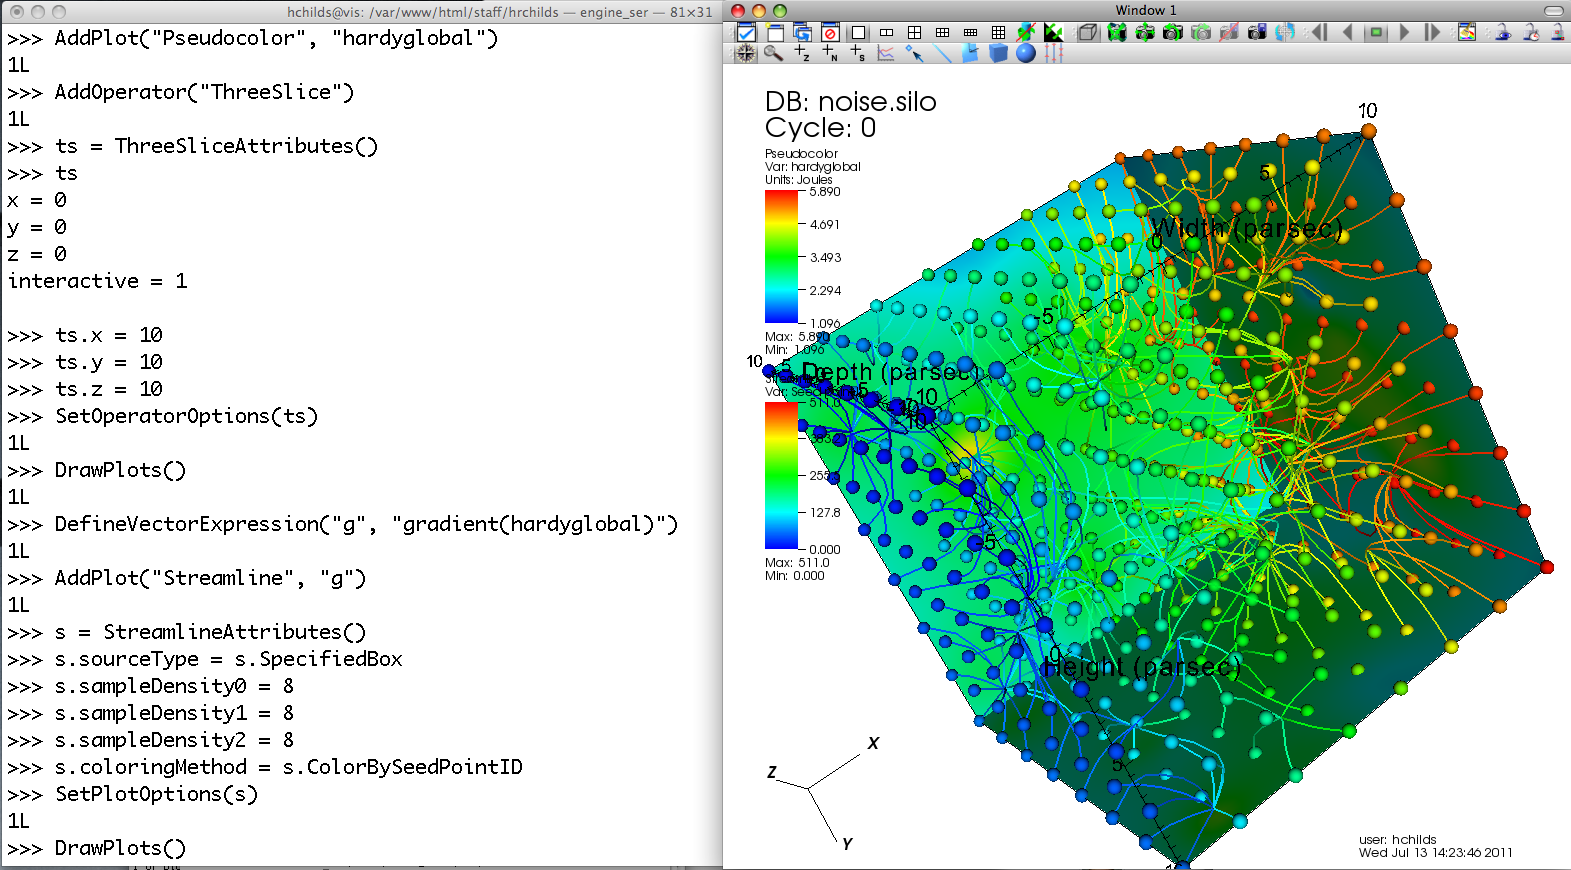
\includegraphics[width=4.8in]{images/teaser}\\[0.5cm]
\hrule
\textsc{\LARGE Version 2.10.0}\\[0.5cm]
\hrule

\date{}
%\maketitle
\end{center}
\end{titlepage}

\pagenumbering{roman}
\tableofcontents
\newpage
\pagenumbering{arabic}


\input{intro.inc}
\input{python.inc}
\input{quickrecipes.inc}
\chapter{Functions}
\input{functions_preamble.inc}

\phantomsection
\addcontentsline{toc}{subsection}{ActivateDatabase}
\noindent {\bf ActivateDatabase}: activates a database that has been previously opened.\\[-3mm]

\noindent {\it Synopsis:} \\ 
\hangindent=\parindent 
\verb!ActivateDatabase(argument) -> integer!\\ [-3mm]

\noindent {\it Arguments:} \\ 
\hangindent=\parindent 
\begin{tabular}{lp{9cm}}
\verb!argument! & A string object containing the name of the database to be activated. \\
\end{tabular} \\[-2mm]


\noindent {\it Returns:} \\ 
\hangindent=\parindent ActivateDatabase returns 1 on success and 0 on failure. \\[-3mm] 

\noindent {\it Description:} \\ 
\hangindent=\parindent The ActivateDatabase function is used to set the active database to a database that has been previously opened. The ActivateDatabase function only works when you are using it to activate a database that you have previously opened. You do not need to use this function unless you frequently toggle between more than one database when making plots or changing time states. While the OpenDatabase function can also be used to set the active database, the ActivateDatabase function does not have any side effects that would cause the time state for the new active database to be changed. \\[-3mm] 

\noindent {\it Example:}\\[-6mm]
\begin{verbatim}% visit -cli
dbs = ("/usr/gapps/visit/data/wave.visit", \
"/usr/gapps/visit/data/curv3d.silo")
OpenDatabase(dbs[0], 17)
AddPlot("Pseudocolor", "u")
DrawPlots()
OpenDatabase(dbs[1])
AddPlot("Pseudocolor", "u")
DrawPlots()
# Let's add another plot from the first database.
ActivateDatabase(dbs[0])
AddPlot("Mesh", "quadmesh")
DrawPlots()
\end{verbatim}
\newpage


\phantomsection
\addcontentsline{toc}{subsection}{AddArgument}
\noindent {\bf AddArgument}: add an argument to the viewer's command line argument list.\\[-3mm]

\noindent {\it Synopsis:} \\ 
\hangindent=\parindent 
\verb!AddArgument(argument)!\\ [-3mm]

\noindent {\it Arguments:} \\ 
\hangindent=\parindent 
\begin{tabular}{lp{9cm}}
\verb!argument! & A string object that is added to the viewer's command line argument list. \\
\end{tabular} \\[-2mm]


\noindent {\it Returns:} \\ 
\hangindent=\parindent AddArgument does not return a value. \\[-3mm] 

\noindent {\it Description:} \\ 
\hangindent=\parindent The AddArgument function is used to add extra command line arguments to VisIt's viewer. This is only useful when VisIt's Python interface is imported into a stand$-$alone Python interpreter because the AddArgument function must be called before the viewer is launched. The AddArgument function has no effect when used in VisIt's cli program because the viewer is automatically launched before any commands are processed. \\[-3mm] 

\noindent {\it Example:}\\[-6mm]
\begin{verbatim}import visit
visit.AddArgument("-nowin") # Add the -nowin argument to the viewer.
\end{verbatim}
\newpage


\phantomsection
\addcontentsline{toc}{subsection}{AddMachineProfile}
\noindent {\bf AddMachineProfile}: <description>\\[-3mm]

\noindent {\it Synopsis:} \\ 
\hangindent=\parindent 
\verb!AddMachineProfile(MachineProfile) -> integer!\\ [-3mm]

\noindent {\it Arguments:} \\ 
\hangindent=\parindent 
\begin{tabular}{ll}
\verb!MachineProfile! &  \\
\end{tabular} \\[-2mm]


\noindent {\it Description:} \\ 
\hangindent=\parindent Sets the input machine profile in the HostProfileList, replaces if one already exists Otherwise adds to the list \\[-3mm] 

\newpage


\phantomsection
\addcontentsline{toc}{subsection}{AddOperator}
\noindent {\bf AddOperator}: adds the named operator to the active plots.\\[-3mm]

\noindent {\it Synopsis:} \\ 
\hangindent=\parindent 
\verb!AddOperator(operator) -> integer!\\ 
\verb!AddOperator(operator, all) -> integer!\\ [-3mm]

\noindent {\it Arguments:} \\ 
\hangindent=\parindent 
\begin{tabular}{lp{9cm}}
\verb!operator! & This is a string containing the name of the operator to be applied. \\
\verb!all! & This is an optional integer argument that applies the operator to all plots if the value of the argument is not zero. \\
\end{tabular} \\[-2mm]


\noindent {\it Returns:} \\ 
\hangindent=\parindent The AddOperator function returns an integer value of 1 for success and 0 for failure. \\[-3mm] 

\noindent {\it Description:} \\ 
\hangindent=\parindent The AddOperator function adds a VisIt operator to the active plots. The operator argument is a string containing the name of the operator to be added to the active plots. The operatore name must be a valid operator plugin name that is a member of the tuple returned by the OperatorPlugins function. The all argument is an integer that determines whether or not the operator is applied to all plots. If the all argument is not provided, the operator is only added to active plots. Once the AddOperator function is called, the desired operator is added to all active plots unless the all argument is a non$-$zero value. When the all argument is a non$-$zero value, the operator is applied to all plots regardless of whether or not they are selected. Operator attributes are set through the SetOperatorOptions function. \\[-3mm] 

\noindent {\it Example:}\\[-6mm]
\begin{verbatim}% visit -cli
OpenDatabase("/usr/gapps/visit/data/globe.silo")
AddPlot("Pseudocolor", "u")
AddPlot("Mesh", "mesh1")
AddOperator("Slice", 1) # Slice both plots
DrawPlots()
\end{verbatim}
\newpage


\phantomsection
\addcontentsline{toc}{subsection}{AddPlot}
\noindent {\bf AddPlot}: creates a new plot.\\[-3mm]

\noindent {\it Synopsis:} \\ 
\hangindent=\parindent 
\verb!AddPlot(plotType, variableName) -> integer!\\ 
\verb!AddPlot(plotType, variableName, inheritSIL) -> integer!\\
\verb!AddPlot(plotType, variableName, inheritSIL,\ ! \\ 
\verb!     applyOperators) -> integer!\\ [-3mm]

\noindent {\it Arguments:} \\ 
\hangindent=\parindent 
\begin{tabular}{lp{9cm}}
\verb!plotType! & This is a string containing the name of a valid plot plugin type. \\
\verb!variableName ! & This is a string containing a valid variable name for the open database. \\
\verb!inheritSIL! & This is an integer flag indicating whether the plot should inherit the active plot's SIL restriction. \\
\verb!applyOperators! & This is an integer flag indicating whether the operators from the active plot should be applied to the new plot. \\
\end{tabular} \\[-2mm]


\noindent {\it Returns:} \\ 
\hangindent=\parindent The AddPlot function returns an integer value of 1 for success and 0 for failure. \\[-3mm] 

\noindent {\it Description:} \\ 
\hangindent=\parindent The AddPlot function creates a new plot of the specified type using a variable from the open database. The plotType argument is a string that contains the name of a valid plot plugin type which must be a member of the string tuple that is returned by the PlotPlugins function. The variableName argument is a string that contains the name of a variable in the open database. After the AddPlot function is called, a new plot is created and it is made the sole active plot. \\[-3mm] 

\noindent {\it Example:}\\[-6mm]
\begin{verbatim}% visit -cli
OpenDatabase("/usr/gapps/visit/data/globe.silo")
AddPlot("Subset", "mat1") # Create a subset plot
DrawPlots()
\end{verbatim}
\newpage


\phantomsection
\addcontentsline{toc}{subsection}{AddWindow}
\noindent {\bf AddWindow}: creates a new visualization window.\\[-3mm]

\noindent {\it Synopsis:} \\ 
\hangindent=\parindent 
\verb!AddWindow()!\\ [-3mm]

\noindent {\it Returns:} \\ 
\hangindent=\parindent The AddWindow function does not a return value. \\[-3mm] 

\noindent {\it Description:} \\ 
\hangindent=\parindent The AddWindow function creates a new visualization window and makes it the active window. This function can be used to create up to 16 visualization windows. After that, the AddWindow function has no effect. \\[-3mm] 

\noindent {\it Example:}\\[-6mm]
\begin{verbatim}import visit
visit.Launch()
visit.AddWindow() # Create window #2
visit.AddWindow() # Create window #3
\end{verbatim}
\newpage


\phantomsection
\addcontentsline{toc}{subsection}{AlterDatabaseCorrelation}
\noindent {\bf AlterDatabaseCorrelation}: alters a specific database correlation.\\[-3mm]

\noindent {\it Synopsis:} \\ 
\hangindent=\parindent 
\verb!AlterDatabaseCorrelation(name, databases, method) -> integer!\\ [-3mm]

\noindent {\it Arguments:} \\ 
\hangindent=\parindent 
\begin{tabular}{lp{9cm}}
\verb!name! & The name argument must be a string object containing the name of the database correlation to be altered. \\
\verb!databases! & The databases argument must be a tuple or list of strings containing the fully qualified database names to be used in the database correlation. \\
\verb!method! & The method argument must be an integer in the range [0,3]. \\
\end{tabular} \\[-2mm]


\noindent {\it Returns:} \\ 
\hangindent=\parindent The AlterDatabaseCorrelation function returns 1 on success and 0 on failure. \\[-3mm] 

\noindent {\it Description:} \\ 
\hangindent=\parindent The AlterDatabaseCorrelation method alters an existing database correlation. A database correlation is a VisIt construct that relates the time states for two or more databases in some way. You would use the AlterDatabaseCorrelation function if you wanted to change the list of databases used in a database correlation or if you wanted to change how the databases are related $-$ the correlation method. The name argument is a string that is the name of the database correlation to be altered. If the name that you pass is not a valid database correlation then the AlterDatabaseCorrelation function fails. The databases argument is a list or tuple of string objects containing the fully$-$qualified (host:/path/filename) names of the databases to be involved in the database query. The method argument allows you to specify a database correlation method. \\

\begin{tabular}{|l|l|}
\hline
\verb!Correlation method! & Value \\
\hline \hline
\verb!IndexForIndexCorrelation! & 0 \\
\verb!StretchedIndexCorrelation! & 1 \\
\verb!TimeCorrelation! & 2 \\
\verb!CycleCorrelation! & 3 \\
\hline
\end{tabular} \\[-2mm]
\\[-3mm] 

\noindent {\it Example:}\\[-6mm]
\begin{verbatim}dbs = ("/usr/gapps/visit/data/wave.visit", \
"/usr/gapps/visit/data/wave*.silo database")
OpenDatabase(dbs[0])
AddPlot("Pseudocolor", "pressure")
OpenDatabase(dbs[1])
AddPlot("Pseudocolor", "d")
# VisIt created an index for index database correlation but we 
# want a cycle correlation.
AlterDatabaseCorrelation("Correlation01", dbs, 3)
\end{verbatim}
\newpage


\phantomsection
\addcontentsline{toc}{subsection}{ApplyNamedSelection}
\noindent {\bf ApplyNamedSelection}: applies a named selection to the active plot.\\[-3mm]

\noindent {\it Synopsis:} \\ 
\hangindent=\parindent 
\verb!ApplyNamedSelection(name) -> integer!\\ [-3mm]

\noindent {\it Arguments:} \\ 
\hangindent=\parindent 
\begin{tabular}{lp{9cm}}
\verb!name! & The name of a named selection.  (This should have been previously created with a CreateNamedSelection call.) \\
\end{tabular} \\[-2mm]


\noindent {\it Returns:} \\ 
\hangindent=\parindent The ApplyNamedSelection function returns 1 for success and 0 for failure. \\[-3mm] 

\noindent {\it Description:} \\ 
\hangindent=\parindent Named Selections allow you to select a group of elements (or particles). One typically creates a named selection from a group of elements and then later applies the named selection to another plot (thus reducing the set of elements displayed to the ones from when the named selection was created). \\[-3mm] 

\noindent {\it Example:}\\[-6mm]
\begin{verbatim}% visit -cli
db = "/usr/gapps/visit/data/wave*.silo database"
OpenDatabase(db)
AddPlot("Pseudocolor", "pressure")
AddOperator("Clip")
c = ClipAttributes()
c.plane1Origin = (0,0.6,0)
c.plane1Normal = (0,-1,0)
SetOperatorOption(c)
DrawPlots()
CreateNamedSelection("els_above_at_time_0")
SetTimeSliderState(40)
RemoveLastOperator()
ApplyNamedSelection("els_above_at_time_0")
\end{verbatim}
\newpage


\phantomsection
\addcontentsline{toc}{subsection}{ChangeActivePlotsVar}
\noindent {\bf ChangeActivePlotsVar}: changes the variable for the active plots\\[-3mm]

\noindent {\it Synopsis:} \\ 
\hangindent=\parindent 
\verb!ChangeActivePlotsVar(variableName) -> integer!\\ [-3mm]

\noindent {\it Arguments:} \\ 
\hangindent=\parindent 
\begin{tabular}{ll}
\verb!variableName! & The name of the new plot variable. \\
\end{tabular} \\[-2mm]


\noindent {\it Returns:} \\ 
\hangindent=\parindent The ChangeActivePlotsVar function returns an integer value of 1 for success and 0 for failure. \\[-3mm] 

\noindent {\it Description:} \\ 
\hangindent=\parindent The ChangeActivePlotsVar function changes the plotted variable for the active plots. This is a useful way to change what is being visualized without having to delete and recreate the current plots. The variableName argument is a string that contains the name of a variable in the open database. \\[-3mm] 

\noindent {\it Example:}\\[-6mm]
\begin{verbatim}% visit -cli
OpenDatabase("/usr/gapps/visit/data/globe.silo")
AddPlot("Pseudocolor", "u")
DrawPlots()
SaveWindow()
ChangeActivePlotsVar("v")
\end{verbatim}
\newpage


\phantomsection
\addcontentsline{toc}{subsection}{CheckForNewStates}
\noindent {\bf CheckForNewStates}: checks the specified database for new time states.\\[-3mm]

\noindent {\it Synopsis:} \\ 
\hangindent=\parindent 
\verb!CheckForNewStates(name) -> integer!\\ [-3mm]

\noindent {\it Arguments:} \\ 
\hangindent=\parindent 
\begin{tabular}{lp{9cm}}
\verb!name! & The name argument must be a string that contains the name of a database that has been opened previously. \\
\end{tabular} \\[-2mm]


\noindent {\it Returns:} \\ 
\hangindent=\parindent The CheckForNewStates function returns 1 for success and 0 for failure. \\[-3mm] 

\noindent {\it Description:} \\ 
\hangindent=\parindent Calculations are often run at the same time as some of the preliminary visualization work is being performed. That said, you might be visualizing the leading time states of a database that is still being created. If you want to force VisIt to add any new time states that were added since you opened the database, you can use the CheckForNewStates function. The name argument must contain the name of a database that has been opened before. \\[-3mm] 

\noindent {\it Example:}\\[-6mm]
\begin{verbatim}% visit -cli
db = "/usr/gapps/visit/data/wave*.silo database"
OpenDatabase(db)
AddPlot("Pseudocolor", "pressure")
DrawPlots()
SetTimeSliderState(TimeSliderGetNStates() - 1)
# More files appear on disk
CheckForNewStates(db)
SetTimeSliderState(TimeSliderGetNStates() - 1)
\end{verbatim}
\newpage


\phantomsection
\addcontentsline{toc}{subsection}{ChooseCenterOfRotation}
\noindent {\bf ChooseCenterOfRotation}: allows you to interactively pick a new center of rotation.\\[-3mm]

\noindent {\it Synopsis:} \\ 
\hangindent=\parindent 
\verb!ChooseCenterOfRotation() -> integer!\\ 
\verb!ChooseCenterOfRotation(screenX, screenY) -> integer!\\ [-3mm]

\noindent {\it Arguments:} \\ 
\hangindent=\parindent 
\begin{tabular}{lp{9cm}}
\verb!screenX! & The X coordinate of the pick point in normalized [0,1] screen space. \\
\verb!screenY! & The Y cooridinate of the pick point in normalized [0,1] screen space. \\
\end{tabular} \\[-2mm]


\noindent {\it Returns:} \\ 
\hangindent=\parindent The ChooseCenterOfRotation function returns 1 if successful and 0 if it fails. \\[-3mm] 

\noindent {\it Description:} \\ 
\hangindent=\parindent The ChooseCenterOfRotation function allows you to pick a new center of rotation, which is the point about which plots are rotated when you interactively rotate plots. The function can either take zero arguments, in which case you must interactively pick on plots, or it can take two arguments that correspond to the X and Y coordinates of the desired pick point in normalized screen space. When using the two argument version of the ChooseCenterOfRotation function, the X and Y values are floating point values in the range [0,1]. If the ChooseCenterOfRotation function is able to actually pick on plots, yes there must be plots in the vis window, then the center of rotation is updated and the new value is printed to the console. \\[-3mm] 

\noindent {\it Example:}\\[-6mm]
\begin{verbatim}% visit -cli
OpenDatabase("/usr/gapps/visit/data/globe.silo")
AddPlots("Pseudocolor", "u")
DrawPlots()
# Interactively choose the center of rotation
ChooseCenterOfRotation()
# Choose a center of rotation using normalized screen 
# coordinates and print the value.
ResetView()
ChooseCenterOfRotation(0.5, 0.3)
print "The new center of rotation is:", GetView3D().centerOfRotation
\end{verbatim}
\newpage


\phantomsection
\addcontentsline{toc}{subsection}{ClearAllWindows}
\noindent {\bf ClearAllWindows}: clears visualization windows of plots.\\[-3mm]

\noindent {\it Synopsis:} \\ 
\hangindent=\parindent 
\verb!ClearAllWindows() -> integer!\\ 
\verb!ClearWindow() -> integer!\\ [-3mm]

\noindent {\it Returns:} \\ 
\hangindent=\parindent 1 on success, 0 on failure. \\[-3mm] 

\noindent {\it Description:} \\ 
\hangindent=\parindent The ClearWindow function is used to clear out the plots from the active visualization window. The plots are removed from the visualization window but are left in the plot list so that subsequent calls to the DrawPlots function regenerate the plots in the plot list. The ClearAllWindows function preforms the same work as the ClearWindow function except that all windows are cleared of their plots. \\[-3mm] 

\noindent {\it Example:}\\[-6mm]
\begin{verbatim}% visit -cli
OpenDatabase("/usr/gapps/visit/data/globe.silo")
AddPlot("Pseudocolor", "u")
DrawPlots()
AddWindow()
SetActiveWindow(2) # Make window 2 active
OpenDatabase("/usr/gapps/visit/data/globe.silo")
AddPlot("Subset", "mat1")
DrawPlots()
ClearWindow() # Clear the plots in window 2.
DrawPlots() # Redraw the plots in window 2.
ClearAllWindows() # Clear the plots from all windows.
\end{verbatim}
\newpage


\phantomsection
\addcontentsline{toc}{subsection}{ClearCache}
\noindent {\bf ClearCache}: clears the compute engine's network cache.\\[-3mm]

\noindent {\it Synopsis:} \\ 
\hangindent=\parindent 
\verb!ClearCache(host) -> integer!\\ 
\verb!ClearCache(host, simulation) -> integer!\\ 
\verb!ClearCacheForAllEngines() -> integer!\\ [-3mm]

\noindent {\it Arguments:} \\ 
\hangindent=\parindent 
\begin{tabular}{lp{9cm}}
\verb!host! & The name of the computer where the compute engine is running. \\
\verb!simulation! & The name of the simulation being processed by the compute engine. \\
\end{tabular} \\[-2mm]


\noindent {\it Returns:} \\ 
\hangindent=\parindent The ClearCache and ClearCacheForAllEngines functions return 1 on success and 0 on failure. \\[-3mm] 

\noindent {\it Description:} \\ 
\hangindent=\parindent Sometimes during extended VisIt runs, you might want to periodically clear the compute engine's network cache to reduce the amount of memory being used by the compute engine. Clearing the network cache is also useful when you want to change what the compute engine is working on. For example, you might process a large database and then decide to process another large database. Clearing the network cache beforehand will free up more resources for the compute engine so it can more efficiently process the new database. The host argument is a string object containing the name of the computer on which the compute engine is running. The simulation argument is optional and only applies to when you want to instruct a simulation that is acting as a VisIt compute engine to clear its network cache. If you want to tell more than one compute engine to clear its cache without having to call ClearCache multiple times, you can use the ClearCacheForAllEngines function. \\[-3mm] 

\noindent {\it Example:}\\[-6mm]
\begin{verbatim}%visit -cli
OpenDatabase("localhost:very_large_database")
# Do a lot of work
ClearCache("localhost")
OpenDatabase(localhost:another_large_database")
# Do more work
OpenDatabase("remotehost:yet_another_database")
# Do more work
ClearCacheForAllEngines()
\end{verbatim}
\newpage


\phantomsection
\addcontentsline{toc}{subsection}{ClearCacheForAllEngines}
\noindent {\bf ClearCacheForAllEngines}: clears the compute engine's network cache.\\[-3mm]

\noindent {\it Synopsis:} \\ 
\hangindent=\parindent 
\verb!ClearCache(host) -> integer!\\ 
\verb!ClearCache(host, simulation) -> integer!\\ 
\verb!ClearCacheForAllEngines() -> integer!\\ [-3mm]

\noindent {\it Arguments:} \\ 
\hangindent=\parindent 
\begin{tabular}{lp{9cm}}
\verb!host! & The name of the computer where the compute engine is running. \\
\verb!simulation! & The name of the simulation being processed by the compute engine. \\
\end{tabular} \\[-2mm]


\noindent {\it Returns:} \\ 
\hangindent=\parindent The ClearCache and ClearCacheForAllEngines functions return 1 on success and 0 on failure. \\[-3mm] 

\noindent {\it Description:} \\ 
\hangindent=\parindent Sometimes during extended VisIt runs, you might want to periodically clear the compute engine's network cache to reduce the amount of memory being used by the compute engine. Clearing the network cache is also useful when you want to change what the compute engine is working on. For example, you might process a large database and then decide to process another large database. Clearing the network cache beforehand will free up more resources for the compute engine so it can more efficiently process the new database. The host argument is a string object containing the name of the computer on which the compute engine is running. The simulation argument is optional and only applies to when you want to instruct a simulation that is acting as a VisIt compute engine to clear its network cache. If you want to tell more than one compute engine to clear its cache without having to call ClearCache multiple times, you can use the ClearCacheForAllEngines function. \\[-3mm] 

\noindent {\it Example:}\\[-6mm]
\begin{verbatim}%visit -cli
OpenDatabase("localhost:very_large_database")
# Do a lot of work
ClearCache("localhost")
OpenDatabase(localhost:another_large_database")
# Do more work
OpenDatabase("remotehost:yet_another_database")
# Do more work
ClearCacheForAllEngines()
\end{verbatim}
\newpage


\phantomsection
\addcontentsline{toc}{subsection}{ClearMacros}
\noindent {\bf ClearMacros}: clear the macros that have been registered using RegisterMacros.\\[-3mm]

\noindent {\it Synopsis:} \\ 
\hangindent=\parindent 
\verb!ClearMacros()!\\ [-3mm]

\noindent {\it Arguments:} \\ 
\hangindent=\parindent 
\begin{tabular}{ll}
\verb!none! &  \\
\end{tabular} \\[-2mm]


\noindent {\it Returns:} \\ 
\hangindent=\parindent The ClearMacros function does not return a value. \\[-3mm] 

\noindent {\it Description:} \\ 
\hangindent=\parindent The ClearMacros function clears out the list of registered macros and sends a message to the gui to clear the buttons from the Macros window. \\[-3mm] 

\noindent {\it Example:}\\[-6mm]
\begin{verbatim}ClearMacros()
\end{verbatim}
\newpage


\phantomsection
\addcontentsline{toc}{subsection}{ClearPickPoints}
\noindent {\bf ClearPickPoints}: clears pick points from the visualization window\\[-3mm]

\noindent {\it Synopsis:} \\ 
\hangindent=\parindent 
\verb!ClearPickPoints()!\\ [-3mm]

\noindent {\it Returns:} \\ 
\hangindent=\parindent The ClearPickPoints function does not return a value. \\[-3mm] 

\noindent {\it Description:} \\ 
\hangindent=\parindent The ClearPickPoints function removes pick points from the active visualization window. Pick points are the letters that are added to the visualization window where the mouse is clicked when the visualization window is in pick mode. \\[-3mm] 

\noindent {\it Example:}\\[-6mm]
\begin{verbatim}% visit -cli
# Put the visualization window into pick mode using the popup 
# menu and add some pick points.
# Clear the pick points.
ClearPickPoints()
\end{verbatim}
\newpage


\phantomsection
\addcontentsline{toc}{subsection}{ClearReferenceLines}
\noindent {\bf ClearReferenceLines}: clears reference lines from the visualization window.\\[-3mm]

\noindent {\it Synopsis:} \\ 
\hangindent=\parindent 
\verb!ClearReferenceLines()!\\ [-3mm]

\noindent {\it Returns:} \\ 
\hangindent=\parindent The ClearReferenceLines function does not return a value. \\[-3mm] 

\noindent {\it Description:} \\ 
\hangindent=\parindent The ClearReferenceLines function removes reference lines from the active visualization window. Reference lines are the lines that are drawn on a plot to show where you have performed lineouts. \\[-3mm] 

\noindent {\it Example:}\\[-6mm]
\begin{verbatim}% visit -cli
OpenDatabase("/usr/gapps/visit/data/curv2d.silo")
AddPlot("Pseudocolor", "d")
Lineout((-3.0, 2.0), (2.0, 4.0), ("default", "u", "v"))
ClearReferenceLines()
\end{verbatim}
\newpage


\phantomsection
\addcontentsline{toc}{subsection}{ClearViewKeyframes}
\noindent {\bf ClearViewKeyframes}: clears any view keyframes that have been set.\\[-3mm]

\noindent {\it Synopsis:} \\ 
\hangindent=\parindent 
\verb!ClearViewKeyframes() -> integer!\\ [-3mm]

\noindent {\it Returns:} \\ 
\hangindent=\parindent The ClearViewKeyframes function returns 1 on success and 0 on failure. \\[-3mm] 

\noindent {\it Description:} \\ 
\hangindent=\parindent The ClearViewKeyframes function clears any view keyframes that may have been set. View keyframes are used to create complex view behavior such as fly$-$throughs when VisIt is in keyframing mode. \\[-3mm] 

\noindent {\it Example:}\\[-6mm]
\begin{verbatim}% visit -cli
OpenDatabase("/usr/gapps/visit/data/globe.silo")
AddPlot("Pseudocolor", "u")
k = KeyframeAttributes()
k.enabled, k.nFrames, k.nFramesWasUserSet = 1,10,1
SetKeyframeAttributes(k)
DrawPlots()
SetViewKeyframe()
v1 = GetView3D()
v1.viewNormal = (-0.66609, 0.337227, 0.665283)
v1.viewUp = (0.157431, 0.935425, -0.316537)
SetView3D(v1)
SetTimeSliderState(9)
SetViewKeyframe()
ToggleCameraViewMode()
for i in range(10):
SetTimeSliderState(i)
ClearViewKeyframes()
\end{verbatim}
\newpage


\phantomsection
\addcontentsline{toc}{subsection}{ClearWindow}
\noindent {\bf ClearWindow}: clears visualization windows of plots.\\[-3mm]

\noindent {\it Synopsis:} \\ 
\hangindent=\parindent 
\verb!ClearAllWindows() -> integer!\\ 
\verb!ClearWindow() -> integer!\\ [-3mm]

\noindent {\it Returns:} \\ 
\hangindent=\parindent 1 on success, 0 on failure. \\[-3mm] 

\noindent {\it Description:} \\ 
\hangindent=\parindent The ClearWindow function is used to clear out the plots from the active visualization window. The plots are removed from the visualization window but are left in the plot list so that subsequent calls to the DrawPlots function regenerate the plots in the plot list. The ClearAllWindows function preforms the same work as the ClearWindow function except that all windows are cleared of their plots. \\[-3mm] 

\noindent {\it Example:}\\[-6mm]
\begin{verbatim}% visit -cli
OpenDatabase("/usr/gapps/visit/data/globe.silo")
AddPlot("Pseudocolor", "u")
DrawPlots()
AddWindow()
SetActiveWindow(2) # Make window 2 active
OpenDatabase("/usr/gapps/visit/data/globe.silo")
AddPlot("Subset", "mat1")
DrawPlots()
ClearWindow() # Clear the plots in window 2.
DrawPlots() # Redraw the plots in window 2.
ClearAllWindows() # Clear the plots from all windows.
\end{verbatim}
\newpage


\phantomsection
\addcontentsline{toc}{subsection}{CloneWindow}
\noindent {\bf CloneWindow}: creates a new window that has the same plots, annotations, lights, and\\[-3mm]

\noindent {\it Synopsis:} \\ 
\hangindent=\parindent 
\verb!CloneWindow() -> integer!\\ [-3mm]

\noindent {\it Returns:} \\ 
\hangindent=\parindent The CloneWindow function returns an integer value of 1 for success and 0 for failure. \\[-3mm] 

\noindent {\it Description:} \\ 
\hangindent=\parindent The CloneWindow function tells the viewer to create a new window, based on the active window, that contains the same plots, annotations, lights, and view as the active window. This function is useful for when you have a window set up like you want and then want to do the same thing in another window using a different database. You can first clone the window and then replace the database. \\[-3mm] 

\noindent {\it Example:}\\[-6mm]
\begin{verbatim}% visit -cli
OpenDatabase("/usr/gapps/visit/data/globe.silo")
AddPlot("Pseudocolor", "u")
DrawPlots()
v = ViewAttributes()
v.camera = (-0.505893, 0.32034, 0.800909)
v.viewUp = (0.1314, 0.946269, -0.295482)
v.parallelScale = 14.5472
v.nearPlane = -34.641
v.farPlane = 34.641
v.perspective = 1
SetView3D() # Set the view
a = AnnotationAttributes()
a.backgroundColor = (0, 0, 255, 255)
SetAnnotationAttributes(a) # Set the annotation properties
CloneWindow() # Create a clone of the active window
DrawPlots() # Make the new window draw its plots
\end{verbatim}
\newpage


\phantomsection
\addcontentsline{toc}{subsection}{Close}
\noindent {\bf Close}: closes the viewer.\\[-3mm]

\noindent {\it Synopsis:} \\ 
\hangindent=\parindent 
\verb!Close()!\\ [-3mm]

\noindent {\it Arguments:} \\ 
\hangindent=\parindent 
\begin{tabular}{ll}
\verb!none! &  \\
\end{tabular} \\[-2mm]


\noindent {\it Returns:} \\ 
\hangindent=\parindent The Close function does not return a value. \\[-3mm] 

\noindent {\it Description:} \\ 
\hangindent=\parindent The Close function terminates VisIt's viewer. This is useful for Python scripts that only need access to VisIt's capabilties for a short time before closing VisIt. \\[-3mm] 

\noindent {\it Example:}\\[-6mm]
\begin{verbatim}import visit
visit.Launch()
visit.Close() # Close the viewer
\end{verbatim}
\newpage


\phantomsection
\addcontentsline{toc}{subsection}{CloseComputeEngine}
\noindent {\bf CloseComputeEngine}: closes the compute engine running on a specified host.\\[-3mm]

\noindent {\it Synopsis:} \\ 
\hangindent=\parindent 
\verb!CloseComputeEngine() -> integer!\\ 
\verb!CloseComputeEngine(hostName) -> integer!\\ 
\verb!CloseComputeEngine(hostName, simulation) -> integer!\\ [-3mm]

\noindent {\it Arguments:} \\ 
\hangindent=\parindent 
\begin{tabular}{lp{9cm}}
\verb!hostName! & Optional name of the computer on which the compute engine is running. \\
\verb!simulation! & Optional name of a simulation. \\
\end{tabular} \\[-2mm]


\noindent {\it Returns:} \\ 
\hangindent=\parindent The CloseComputeEngine function returns an integer value of 1 for success and 0 for failure. \\[-3mm] 

\noindent {\it Description:} \\ 
\hangindent=\parindent The CloseComputeEngine function tells the viewer to close the compute engine running a specified host. The hostName argument is a string that contains the name of the computer where the compute engine is running. The hostName argument can also be the name "localhost" if you want to close the compute engine on the local machine without having to specify its name. It is not necessary to provide the hostName argument. If the argument is omitted, the first compute engine in the engine list will be closed. The simulation argument can be provided if you want to close a connection to a simulation that is acting as a VisIt compute engine. A compute engine can be launched again by creating a plot or by calling the OpenComputeEngine function. \\[-3mm] 

\noindent {\it Example:}\\[-6mm]
\begin{verbatim}% visit -cli
OpenDatabase("/usr/gapps/visit/data/globe.silo") # Launches an engine
AddPlot("Pseudocolor", "u")
DrawPlots()
CloseComputeEngine() # Close the compute engine
\end{verbatim}
\newpage


\phantomsection
\addcontentsline{toc}{subsection}{CloseDatabase}
\noindent {\bf CloseDatabase}: closes the specified database and frees up resources associated with it.\\[-3mm]

\noindent {\it Synopsis:} \\ 
\hangindent=\parindent 
\verb!CloseDatabase(name) -> integer!\\ [-3mm]

\noindent {\it Arguments:} \\ 
\hangindent=\parindent 
\begin{tabular}{lp{9cm}}
\verb!name! & A string object containing the name of the database to close. \\
\end{tabular} \\[-2mm]


\noindent {\it Returns:} \\ 
\hangindent=\parindent The CloseDatabase function returns 1 on success and 0 on failure. \\[-3mm] 

\noindent {\it Description:} \\ 
\hangindent=\parindent The CloseDatabase function is used to close a specified database and free all resources that were devoted to keeping the database open. This function has an effect similar to ClearCache but it does more in that in addition to clearing the compute engine's cache, which it only does for the specified database, it also removes all references to the specified database from tables of cached metadata, etc. Note that the CloseDatabase function will fail and the database will not be closed if any plots reference the specified database. \\[-3mm] 

\noindent {\it Example:}\\[-6mm]
\begin{verbatim}% visit -cli
db = "/usr/gapps/visit/data/globe.silo"
OpenDatabase(db)
AddPlot("Pseudocolor", "u")
DrawPlots()
print "This won't work: retval = %d" % CloseDatabase(db)
DeleteAllPlots()
print "Now it works: retval = %d" % CloseDatabase(db)
\end{verbatim}
\newpage


\phantomsection
\addcontentsline{toc}{subsection}{ColorTableNames}
\noindent {\bf ColorTableNames}: returns a tuple of color table names.\\[-3mm]

\noindent {\it Synopsis:} \\ 
\hangindent=\parindent 
\verb!ColorTableNames() -> tuple!\\ [-3mm]

\noindent {\it Returns:} \\ 
\hangindent=\parindent The ColorTableNames function returns a tuple of strings containing the names of the color tables that have been defined. \\[-3mm] 

\noindent {\it Description:} \\ 
\hangindent=\parindent The ColorTableNames function returns a tuple of strings containing the names of the color tables that have been defined. This method can be used in case you want to iterate over several color tables. \\[-3mm] 

\noindent {\it Example:}\\[-6mm]
\begin{verbatim}% visit -cli 
OpenDatabase("/usr/gapps/visit/data/curv2d.silo")
AddPlot("Pseudocolor", "u")
DrawPlots()
for ct in ColorTableNames():
p = PseudocolorAttributes()
p.colorTableName = ct
SetPlotOptions(p)
\end{verbatim}
\newpage


\phantomsection
\addcontentsline{toc}{subsection}{ConstructDataBinning}
\noindent {\bf ConstructDataBinning}: constructs a data binning\\[-3mm]

\noindent {\it Synopsis:} \\ 
\hangindent=\parindent 
\verb!ConstructDataBinning(i) -> integer!\\ [-3mm]

\noindent {\it Arguments:} \\ 
\hangindent=\parindent 
\begin{tabular}{lp{9cm}}
\verb!i! & An object of type ConstructDataBinningAttributes. This object specifies the options for constructing a data binning. \\
\end{tabular} \\[-2mm]


\noindent {\it Returns:} \\ 
\hangindent=\parindent Returns 1 on success, 0 on failure. \\[-3mm] 

\noindent {\it Description:} \\ 
\hangindent=\parindent The ConstructDataBinning function creates a data binning function for the active plot. Data Binnings place data from a data set into bins and reduce that data. They are used to either be incorporated with expressions to make new derived quantities or to be directly visualized. \\[-3mm] 

\noindent {\it Example:}\\[-6mm]
\begin{verbatim}% visit -cli
OpenDatabase("/usr/gapps/visit/data/curv3d.silo")
AddPlot("Pseudocolor", "d")
DrawPlots()
# Set the construct data binning attributes.
i = ConstructDataBinningAttributes()
i.name = "db1"
i.binningScheme = i.Uniform
i.varnames = ("u", "w")
i.binBoundaries = (-1, 1, -1, 1) # minu, maxu, minw, maxw
i.numSamples = (25, 25)
i.reductionOperator = i.Average
i.varForReductionOperator = "v"
ConstructDataBinning(i)
# Example of binning using spatial coordinates
i.varnames = ("X", "u") # X is added as a placeholder to maintain indexing
i.binType = (1, 0) # 1 = X, 2 = Y, 3 = Z, 0 = variable
\end{verbatim}
\newpage


\phantomsection
\addcontentsline{toc}{subsection}{CopyAnnotationsToWindow}
\noindent {\bf CopyAnnotationsToWindow}: copies attributes from one visualization window to another visualization\\[-3mm]

\noindent {\it Synopsis:} \\ 
\hangindent=\parindent 
\verb!CopyAnnotationsToWindow(source, dest) -> integer!\\ 
\verb!CopyLightingToWindow(source, dest) -> integer!\\ 
\verb!CopyViewTowindow(source, dest) -> integer!\\ 
\verb!CopyPlotsToWindow(source, dest) -> integer!\\ [-3mm]

\noindent {\it Arguments:} \\ 
\hangindent=\parindent 
\begin{tabular}{lp{9cm}}
\verb!source! & The index (an integer from 1 to 16) of the source window. \\
\verb!dest! & The index (an integer from 1 to 16) of the destination window. \\
\end{tabular} \\[-2mm]


\noindent {\it Returns:} \\ 
\hangindent=\parindent The Copy functions return an integer value of 1 for success and 0 for failure. \\[-3mm] 

\noindent {\it Description:} \\ 
\hangindent=\parindent The Copy functions copy attributes from one visualization window to another visualization window. The CopyAnnotationsToWindow function copies the annotations from a source visualization window to a destination visualization window while the CopyLightingAttributes function copies lighting and the CopyViewToWindow function copies the view. The CopyPlotsToWindow function copies the plots from one visualization window to another visualization window but does not also force plots to generate so after copying plots with the CopyPlotsToWindow function, you should also call the DrawPlots function. \\[-3mm] 

\noindent {\it Example:}\\[-6mm]
\begin{verbatim}% visit -cli
OpenDatabase("/usr/gapps/visit/data/globe.silo")
AddPlot("Pseudocolor", "u")
DrawPlots()
AddWindow()
SetActiveWindow(2)
OpenDatabase("/usr/gapps/visit/data/globe.silo")
AddPlot("Mesh", "mesh1")
# Copy window 1's Pseudocolor plot to window 2.
CopyPlotsToWindow(1, 2) 
DrawPlots() # Window 2 will have 2 plots
# Spin the plots around in window 2 using the mouse.
CopyViewToWindow(2, 1) # Copy window 2's view to window 1.
\end{verbatim}
\newpage


\phantomsection
\addcontentsline{toc}{subsection}{CopyLightingToWindow}
\noindent {\bf CopyLightingToWindow}: copies attributes from one visualization window to another visualization\\[-3mm]

\noindent {\it Synopsis:} \\ 
\hangindent=\parindent 
\verb!CopyAnnotationsToWindow(source, dest) -> integer!\\ 
\verb!CopyLightingToWindow(source, dest) -> integer!\\ 
\verb!CopyViewTowindow(source, dest) -> integer!\\ 
\verb!CopyPlotsToWindow(source, dest) -> integer!\\ [-3mm]

\noindent {\it Arguments:} \\ 
\hangindent=\parindent 
\begin{tabular}{lp{9cm}}
\verb!source! & The index (an integer from 1 to 16) of the source window. \\
\verb!dest! & The index (an integer from 1 to 16) of the destination window. \\
\end{tabular} \\[-2mm]


\noindent {\it Returns:} \\ 
\hangindent=\parindent The Copy functions return an integer value of 1 for success and 0 for failure. \\[-3mm] 

\noindent {\it Description:} \\ 
\hangindent=\parindent The Copy functions copy attributes from one visualization window to another visualization window. The CopyAnnotationsToWindow function copies the annotations from a source visualization window to a destination visualization window while the CopyLightingAttributes function copies lighting and the CopyViewToWindow function copies the view. The CopyPlotsToWindow function copies the plots from one visualization window to another visualization window but does not also force plots to generate so after copying plots with the CopyPlotsToWindow function, you should also call the DrawPlots function. \\[-3mm] 

\noindent {\it Example:}\\[-6mm]
\begin{verbatim}% visit -cli
OpenDatabase("/usr/gapps/visit/data/globe.silo")
AddPlot("Pseudocolor", "u")
DrawPlots()
AddWindow()
SetActiveWindow(2)
OpenDatabase("/usr/gapps/visit/data/globe.silo")
AddPlot("Mesh", "mesh1")
# Copy window 1's Pseudocolor plot to window 2.
CopyPlotsToWindow(1, 2) 
DrawPlots() # Window 2 will have 2 plots
# Spin the plots around in window 2 using the mouse.
CopyViewToWindow(2, 1) # Copy window 2's view to window 1.
\end{verbatim}
\newpage


\phantomsection
\addcontentsline{toc}{subsection}{CopyPlotsToWindow}
\noindent {\bf CopyPlotsToWindow}: copies attributes from one visualization window to another visualization\\[-3mm]

\noindent {\it Synopsis:} \\ 
\hangindent=\parindent 
\verb!CopyAnnotationsToWindow(source, dest) -> integer!\\ 
\verb!CopyLightingToWindow(source, dest) -> integer!\\ 
\verb!CopyViewTowindow(source, dest) -> integer!\\ 
\verb!CopyPlotsToWindow(source, dest) -> integer!\\ [-3mm]

\noindent {\it Arguments:} \\ 
\hangindent=\parindent 
\begin{tabular}{lp{9cm}}
\verb!source! & The index (an integer from 1 to 16) of the source window. \\
\verb!dest! & The index (an integer from 1 to 16) of the destination window. \\
\end{tabular} \\[-2mm]


\noindent {\it Returns:} \\ 
\hangindent=\parindent The Copy functions return an integer value of 1 for success and 0 for failure. \\[-3mm] 

\noindent {\it Description:} \\ 
\hangindent=\parindent The Copy functions copy attributes from one visualization window to another visualization window. The CopyAnnotationsToWindow function copies the annotations from a source visualization window to a destination visualization window while the CopyLightingAttributes function copies lighting and the CopyViewToWindow function copies the view. The CopyPlotsToWindow function copies the plots from one visualization window to another visualization window but does not also force plots to generate so after copying plots with the CopyPlotsToWindow function, you should also call the DrawPlots function. \\[-3mm] 

\noindent {\it Example:}\\[-6mm]
\begin{verbatim}% visit -cli
OpenDatabase("/usr/gapps/visit/data/globe.silo")
AddPlot("Pseudocolor", "u")
DrawPlots()
AddWindow()
SetActiveWindow(2)
OpenDatabase("/usr/gapps/visit/data/globe.silo")
AddPlot("Mesh", "mesh1")
# Copy window 1's Pseudocolor plot to window 2.
CopyPlotsToWindow(1, 2) 
DrawPlots() # Window 2 will have 2 plots
# Spin the plots around in window 2 using the mouse.
CopyViewToWindow(2, 1) # Copy window 2's view to window 1.
\end{verbatim}
\newpage


\phantomsection
\addcontentsline{toc}{subsection}{CopyViewToWindow}
\noindent {\bf CopyViewToWindow}: copies attributes from one visualization window to another visualization\\[-3mm]

\noindent {\it Synopsis:} \\ 
\hangindent=\parindent 
\verb!CopyAnnotationsToWindow(source, dest) -> integer!\\ 
\verb!CopyLightingToWindow(source, dest) -> integer!\\ 
\verb!CopyViewTowindow(source, dest) -> integer!\\ 
\verb!CopyPlotsToWindow(source, dest) -> integer!\\ [-3mm]

\noindent {\it Arguments:} \\ 
\hangindent=\parindent 
\begin{tabular}{lp{9cm}}
\verb!source! & The index (an integer from 1 to 16) of the source window. \\
\verb!dest! & The index (an integer from 1 to 16) of the destination window. \\
\end{tabular} \\[-2mm]


\noindent {\it Returns:} \\ 
\hangindent=\parindent The Copy functions return an integer value of 1 for success and 0 for failure. \\[-3mm] 

\noindent {\it Description:} \\ 
\hangindent=\parindent The Copy functions copy attributes from one visualization window to another visualization window. The CopyAnnotationsToWindow function copies the annotations from a source visualization window to a destination visualization window while the CopyLightingAttributes function copies lighting and the CopyViewToWindow function copies the view. The CopyPlotsToWindow function copies the plots from one visualization window to another visualization window but does not also force plots to generate so after copying plots with the CopyPlotsToWindow function, you should also call the DrawPlots function. \\[-3mm] 

\noindent {\it Example:}\\[-6mm]
\begin{verbatim}% visit -cli
OpenDatabase("/usr/gapps/visit/data/globe.silo")
AddPlot("Pseudocolor", "u")
DrawPlots()
AddWindow()
SetActiveWindow(2)
OpenDatabase("/usr/gapps/visit/data/globe.silo")
AddPlot("Mesh", "mesh1")
# Copy window 1's Pseudocolor plot to window 2.
CopyPlotsToWindow(1, 2) 
DrawPlots() # Window 2 will have 2 plots
# Spin the plots around in window 2 using the mouse.
CopyViewToWindow(2, 1) # Copy window 2's view to window 1.
\end{verbatim}
\newpage


\phantomsection
\addcontentsline{toc}{subsection}{CreateAnnotationObject}
\noindent {\bf CreateAnnotationObject}: creates an annotation object that can directly manipulate annotations in\\[-3mm]

\noindent {\it Synopsis:} \\ 
\hangindent=\parindent 
\verb!CreateAnnotationObject(annotType) -> annotation object!\\ [-3mm]

\noindent {\it Arguments:} \\ 
\hangindent=\parindent 
\begin{tabular}{lp{9cm}}
\verb!annotType! & A string containing the name of the type of annotation object to create. \\
\end{tabular} \\[-2mm]


\noindent {\it Returns:} \\ 
\hangindent=\parindent CreateAnnotationObject is a factory function that creates annotation objects of different types. The return value, if a valid annotation type is provided, is an annotation object. If the function fails, VisItException is raised. \\[-3mm] 

\noindent {\it Description:} \\ 
\hangindent=\parindent CreateAnnotationObject is a factory function that creates different kinds of annotation objects. The annotType argument is a string containing the name of the type of annotation object to create. Each type of annotation object has different properties that can be set. Setting the different properties of an Annotation objects directly modifes annotations in the vis window. Currently there are 5 types of annotation objects: \\

\begin{tabular}{|l|l|}
\hline
\verb!Annotation type! & String \\
\hline \hline
\verb!2D text annotation! & "Text2D" \\
\verb!3D text annotation! & "Text3D" \\
\verb!Time slider annotation! & "TimeSlider" \\
\verb!Image annotation! & "Image" \\
\verb!Line/arrow annotation! & "Line2D" \\
\hline
\end{tabular} \\[-2mm]
\\[-3mm] 

\noindent {\it Example:}\\[-6mm]
\begin{verbatim}% visit -cli
OpenDatabase("/usr/gapps/visit/data/wave.visit", 17)
AddPlot("Pseudocolor", "pressure")
DrawPlots()
slider = CreateAnnotationObject("TimeSlider")
print slider
slider.startColor = (255,0,0,255)
slider.endColor = (255,255,0,255)
\end{verbatim}
\newpage


\phantomsection
\addcontentsline{toc}{subsection}{CreateDatabaseCorrelation}
\noindent {\bf CreateDatabaseCorrelation}: creates a database correlation.\\[-3mm]

\noindent {\it Synopsis:} \\ 
\hangindent=\parindent 
\verb!CreateDatabaseCorrelation(name, databases, method) -> integer!\\ [-3mm]

\noindent {\it Arguments:} \\ 
\hangindent=\parindent 
\begin{tabular}{lp{9cm}}
\verb!name! & String object containing the name of the database correlation to be created. \\
\verb!databases! & Tuple or list of string objects containing the names of the databases to involve in the database correlation. \\
\verb!method! & An integer in the range [0,3] that determines the correlation method. \\
\end{tabular} \\[-2mm]


\noindent {\it Returns:} \\ 
\hangindent=\parindent The CreateDatabaseCorrelation function returns 1 on success and 0 on failure. \\[-3mm] 

\noindent {\it Description:} \\ 
\hangindent=\parindent The CreateDatabaseCorrelation function creates a database correlation, which is a VisIt construct that relates the time states for two or more databases in some way. You would use the CreateDatabaseCorrelation function if you wanted to put plots from more than one time$-$varying database in the same vis window and then move them both through time in some synchronized way. The name argument is a string that is the name of the database correlation to be created. You will use the name of the database correlation to set the active time slider later so that you can change time states. The databases argument is a list or tuple of string objects containing the fully$-$qualified (host:/path/filename) names of the databases to be involved in the database query. The method argument allows you to specify a database correlation method. \\

\begin{tabular}{|l|l|}
\hline
\verb!Correlation method! & Value \\
\hline \hline
\verb!IndexForIndexCorrelation! & 0 \\
\verb!StretchedIndexCorrelation! & 1 \\
\verb!TimeCorrelation! & 2 \\
\verb!CycleCorrelation! & 3 \\
\hline
\end{tabular} \\[-2mm]
\\

\hangindent=\parindent
Each database correlation has its own time slider that can be used to set the time state of databases that are part of a database correlation. Individual time$-$varying databases have their own trivial database correlation, consisting of only 1 database. When you call the CreateDatabaseCorrelation function, VisIt creates a new time slider with the same name as the database correlation and makes it be the active time slider. \\[-3mm] 

\noindent {\it Example:}\\[-6mm]
\begin{verbatim}% visit -cli
dbs = ("/usr/gapps/visit/data/dbA00.pdb",
"/usr/gapps/visit/data/dbB00.pdb")
OpenDatabase(dbs[0])
AddPlot("FilledBoundary", "material(mesh)")
OpenDatabase(dbs[1])
AddPlot("FilledBoundary", "material(mesh)")
DrawPlots()
CreateDatabaseCorrelation("common", dbs, 1)
# Creating a new database correlation also creates a new time 
# slider and makes it be active.
w = GetWindowInformation()
print "Active time slider: %s" % w.timeSliders[w.activeTimeSlider]
# Animate through time using the "common" database correlation's 
# time slider.
for i in range(TimeSliderGetNStates()):
SetTimeSliderState(i)
\end{verbatim}
\newpage


\phantomsection
\addcontentsline{toc}{subsection}{CreateNamedSelection}
\noindent {\bf CreateNamedSelection}: creates a named selection.\\[-3mm]

\noindent {\it Synopsis:} \\ 
\hangindent=\parindent 
\verb!CreateNamedSelection(name) -> integer!\\ 
\verb!CreateNamedSelection(name, properties) -> integer!\\ [-3mm]

\noindent {\it Arguments:} \\ 
\hangindent=\parindent 
\begin{tabular}{lp{9cm}}
\verb!name! & The name of a named selection. \\
\verb!properties! & This optional argument lets you pass a SelectionProperties object containing the properties that will be used to create the named selection. When this argument is omitted, the named selection will always be associated with the active plot. You can use this argument to set up more complex named selections that may be associated with plots or databases. \\
\end{tabular} \\[-2mm]


\noindent {\it Returns:} \\ 
\hangindent=\parindent The CreateNamedSelection function returns 1 for success and 0 for failure. \\[-3mm] 

\noindent {\it Description:} \\ 
\hangindent=\parindent Named Selections allow you to select a group of elements (or particles). One typically creates a named selection from a group of elements and then later applies the named selection to another plot (thus reducing the set of elements displayed to the ones from when the named selection was created). \\[-3mm] 

\noindent {\it Example:}\\[-6mm]
\begin{verbatim}% visit -cli
db = "/usr/gapps/visit/data/wave*.silo database"
OpenDatabase(db)
AddPlot("Pseudocolor", "pressure")
AddOperator("Clip")
c = ClipAttributes()
c.plane1Origin = (0,0.6,0)
c.plane1Normal = (0,-1,0)
SetOperatorOption(c)
DrawPlots()
CreateNamedSelection("els_above_at_time_0")
SetTimeSliderState(40)
RemoveLastOperator()
ApplyNamedSelection("els_above_at_time_0")
\end{verbatim}
\newpage


\phantomsection
\addcontentsline{toc}{subsection}{DeIconifyAllWindows}
\noindent {\bf DeIconifyAllWindows}: unhides all of the hidden visualization windows.\\[-3mm]

\noindent {\it Synopsis:} \\ 
\hangindent=\parindent 
\verb!DeIconifyAllWindows()!\\ [-3mm]

\noindent {\it Returns:} \\ 
\hangindent=\parindent The DeIconifyAllWindows function does not return a value. \\[-3mm] 

\noindent {\it Description:} \\ 
\hangindent=\parindent The DeIconifyAllWindows function unhides all of the hidden visualization windows. This function is usually called after IconifyAllWindows as a way of making all of the hidden visualization windows visible. \\[-3mm] 

\noindent {\it Example:}\\[-6mm]
\begin{verbatim}% visit -cli
SetWindowLayout(4) # Have 4 windows
IconifyAllWindows()
DeIconifyAllWindows()
\end{verbatim}
\newpage


\phantomsection
\addcontentsline{toc}{subsection}{DefineArrayExpression}
\noindent {\bf DefineArrayExpression}: creates a expression variable.\\[-3mm]

\noindent {\it Synopsis:} \\ 
\hangindent=\parindent 
\verb!DefineMaterialExpression(variableName, expression) -> integer!\\ 
\verb!DefineMeshExpression(variableName, expression) -> integer!\\ 
\verb!DefineScalarExpression(variableName, expression) -> integer!\\ 
\verb!DefineSpeciesExpression(variableName, expression) -> integer!\\ 
\verb!DefineTensorExpression(variableName, expression) -> integer!\\ 
\verb!DefineVectorExpression(variableName, expression) -> integer!\\ 
\verb!DefineArrayExpression(variableName, expression) -> integer!\\ 
\verb!DefineCurveExpression(variableName, expression) -> integer!\\ [-3mm]

\noindent {\it Arguments:} \\ 
\hangindent=\parindent 
\begin{tabular}{ll}
\verb!variableName! & The name of the variable to be created. \\
\verb!expression! & The expression definition. \\
\end{tabular} \\[-2mm]


\noindent {\it Returns:} \\ 
\hangindent=\parindent The DefineExpression functions return 1 on success and 0 on failure. \\[-3mm] 

\noindent {\it Description:} \\ 
\hangindent=\parindent The DefineScalarExpression function creates a new scalar variable based on other variables from the open database. Likewise, the DefineMaterialExpression function creates new material variables, DefineMeshExpression creates new mesh variables, DefineSpeciesExpression creates new species variables, DefineVectorExpression creates new vector variables, DefineTensorExpression creates new tensor variables, and DefineArrayExpression creates new array variables. Expression variables can be plotted like any other variable. The variableName argument is a string that contains the name of the new variable. You can pass the name of an existing expression if you want to provide a new expression definition. The expression argument is a string that contains the definition of the new variable in terms of math operators and pre$-$existing variable names Reference the VisIt User's Manual if you want more information on  creating expressions, such as expression syntax, or a list of built$-$in expression functions. \\[-3mm] 

\noindent {\it Example:}\\[-6mm]
\begin{verbatim}% visit -cli
OpenDatabase("/usr/gapps/visit/data/globe.silo")
DefineScalarExpression("myvar", "sin(u) + cos(w)")
# Plot the scalar expression variable.
AddPlot("Pseudocolor", "myvar")
DrawPlots()
# Plot a vector expression variable.
DefineVectorExpression("myvec", "{u,v,w}")
AddPlot("Vector", "myvec")
DrawPlots()
\end{verbatim}
\newpage


\phantomsection
\addcontentsline{toc}{subsection}{DefineCurveExpression}
\noindent {\bf DefineCurveExpression}: creates a expression variable.\\[-3mm]

\noindent {\it Synopsis:} \\ 
\hangindent=\parindent 
\verb!DefineMaterialExpression(variableName, expression) -> integer!\\ 
\verb!DefineMeshExpression(variableName, expression) -> integer!\\ 
\verb!DefineScalarExpression(variableName, expression) -> integer!\\ 
\verb!DefineSpeciesExpression(variableName, expression) -> integer!\\ 
\verb!DefineTensorExpression(variableName, expression) -> integer!\\ 
\verb!DefineVectorExpression(variableName, expression) -> integer!\\ 
\verb!DefineArrayExpression(variableName, expression) -> integer!\\ 
\verb!DefineCurveExpression(variableName, expression) -> integer!\\ [-3mm]

\noindent {\it Arguments:} \\ 
\hangindent=\parindent 
\begin{tabular}{ll}
\verb!variableName! & The name of the variable to be created. \\
\verb!expression! & The expression definition. \\
\end{tabular} \\[-2mm]


\noindent {\it Returns:} \\ 
\hangindent=\parindent The DefineExpression functions return 1 on success and 0 on failure. \\[-3mm] 

\noindent {\it Description:} \\ 
\hangindent=\parindent The DefineScalarExpression function creates a new scalar variable based on other variables from the open database. Likewise, the DefineMaterialExpression function creates new material variables, DefineMeshExpression creates new mesh variables, DefineSpeciesExpression creates new species variables, DefineVectorExpression creates new vector variables, DefineTensorExpression creates new tensor variables, and DefineArrayExpression creates new array variables. Expression variables can be plotted like any other variable. The variableName argument is a string that contains the name of the new variable. You can pass the name of an existing expression if you want to provide a new expression definition. The expression argument is a string that contains the definition of the new variable in terms of math operators and pre$-$existing variable names Reference the VisIt User's Manual if you want more information on  creating expressions, such as expression syntax, or a list of built$-$in expression functions. \\[-3mm] 

\noindent {\it Example:}\\[-6mm]
\begin{verbatim}% visit -cli
OpenDatabase("/usr/gapps/visit/data/globe.silo")
DefineScalarExpression("myvar", "sin(u) + cos(w)")
# Plot the scalar expression variable.
AddPlot("Pseudocolor", "myvar")
DrawPlots()
# Plot a vector expression variable.
DefineVectorExpression("myvec", "{u,v,w}")
AddPlot("Vector", "myvec")
DrawPlots()
\end{verbatim}
\newpage


\phantomsection
\addcontentsline{toc}{subsection}{DefineMaterialExpression}
\noindent {\bf DefineMaterialExpression}: creates a expression variable.\\[-3mm]

\noindent {\it Synopsis:} \\ 
\hangindent=\parindent 
\verb!DefineMaterialExpression(variableName, expression) -> integer!\\ 
\verb!DefineMeshExpression(variableName, expression) -> integer!\\ 
\verb!DefineScalarExpression(variableName, expression) -> integer!\\ 
\verb!DefineSpeciesExpression(variableName, expression) -> integer!\\ 
\verb!DefineTensorExpression(variableName, expression) -> integer!\\ 
\verb!DefineVectorExpression(variableName, expression) -> integer!\\ 
\verb!DefineArrayExpression(variableName, expression) -> integer!\\ 
\verb!DefineCurveExpression(variableName, expression) -> integer!\\ [-3mm]

\noindent {\it Arguments:} \\ 
\hangindent=\parindent 
\begin{tabular}{ll}
\verb!variableName! & The name of the variable to be created. \\
\verb!expression! & The expression definition. \\
\end{tabular} \\[-2mm]


\noindent {\it Returns:} \\ 
\hangindent=\parindent The DefineExpression functions return 1 on success and 0 on failure. \\[-3mm] 

\noindent {\it Description:} \\ 
\hangindent=\parindent The DefineScalarExpression function creates a new scalar variable based on other variables from the open database. Likewise, the DefineMaterialExpression function creates new material variables, DefineMeshExpression creates new mesh variables, DefineSpeciesExpression creates new species variables, DefineVectorExpression creates new vector variables, DefineTensorExpression creates new tensor variables, and DefineArrayExpression creates new array variables. Expression variables can be plotted like any other variable. The variableName argument is a string that contains the name of the new variable. You can pass the name of an existing expression if you want to provide a new expression definition. The expression argument is a string that contains the definition of the new variable in terms of math operators and pre$-$existing variable names Reference the VisIt User's Manual if you want more information on  creating expressions, such as expression syntax, or a list of built$-$in expression functions. \\[-3mm] 

\noindent {\it Example:}\\[-6mm]
\begin{verbatim}% visit -cli
OpenDatabase("/usr/gapps/visit/data/globe.silo")
DefineScalarExpression("myvar", "sin(u) + cos(w)")
# Plot the scalar expression variable.
AddPlot("Pseudocolor", "myvar")
DrawPlots()
# Plot a vector expression variable.
DefineVectorExpression("myvec", "{u,v,w}")
AddPlot("Vector", "myvec")
DrawPlots()
\end{verbatim}
\newpage


\phantomsection
\addcontentsline{toc}{subsection}{DefineMeshExpression}
\noindent {\bf DefineMeshExpression}: creates a expression variable.\\[-3mm]

\noindent {\it Synopsis:} \\ 
\hangindent=\parindent 
\verb!DefineMaterialExpression(variableName, expression) -> integer!\\ 
\verb!DefineMeshExpression(variableName, expression) -> integer!\\ 
\verb!DefineScalarExpression(variableName, expression) -> integer!\\ 
\verb!DefineSpeciesExpression(variableName, expression) -> integer!\\ 
\verb!DefineTensorExpression(variableName, expression) -> integer!\\ 
\verb!DefineVectorExpression(variableName, expression) -> integer!\\ 
\verb!DefineArrayExpression(variableName, expression) -> integer!\\ 
\verb!DefineCurveExpression(variableName, expression) -> integer!\\ [-3mm]

\noindent {\it Arguments:} \\ 
\hangindent=\parindent 
\begin{tabular}{ll}
\verb!variableName! & The name of the variable to be created. \\
\verb!expression! & The expression definition. \\
\end{tabular} \\[-2mm]


\noindent {\it Returns:} \\ 
\hangindent=\parindent The DefineExpression functions return 1 on success and 0 on failure. \\[-3mm] 

\noindent {\it Description:} \\ 
\hangindent=\parindent The DefineScalarExpression function creates a new scalar variable based on other variables from the open database. Likewise, the DefineMaterialExpression function creates new material variables, DefineMeshExpression creates new mesh variables, DefineSpeciesExpression creates new species variables, DefineVectorExpression creates new vector variables, DefineTensorExpression creates new tensor variables, and DefineArrayExpression creates new array variables. Expression variables can be plotted like any other variable. The variableName argument is a string that contains the name of the new variable. You can pass the name of an existing expression if you want to provide a new expression definition. The expression argument is a string that contains the definition of the new variable in terms of math operators and pre$-$existing variable names Reference the VisIt User's Manual if you want more information on  creating expressions, such as expression syntax, or a list of built$-$in expression functions. \\[-3mm] 

\noindent {\it Example:}\\[-6mm]
\begin{verbatim}% visit -cli
OpenDatabase("/usr/gapps/visit/data/globe.silo")
DefineScalarExpression("myvar", "sin(u) + cos(w)")
# Plot the scalar expression variable.
AddPlot("Pseudocolor", "myvar")
DrawPlots()
# Plot a vector expression variable.
DefineVectorExpression("myvec", "{u,v,w}")
AddPlot("Vector", "myvec")
DrawPlots()
\end{verbatim}
\newpage


\phantomsection
\addcontentsline{toc}{subsection}{DefinePythonExpression}
\noindent {\bf DefinePythonExpression}: defines a new Python Filter Expression.\\[-3mm]

\noindent {\it Synopsis:} \\ 
\hangindent=\parindent
\verb!DefinePythonExpression("myvar",[args],\ ! \\ 
\verb!    source='python filter source ...')!\\
\verb!DefinePythonExpression("myvar",[args],\ ! \\ 
\verb!        source='python filter source ...',type='scalar')!\\
\verb!DefinePythonExpression("myvar",[args],\ ! \\ 
\verb!    file='path/to/python_filter_script.py')!\\ [-3mm]

\noindent {\it Arguments:} \\ 
\hangindent=\parindent 
\begin{tabular}{lp{9cm}}
\verb!name! & The name of the variable to be created. \\
\verb!args! & A tuple (or list) of strings providing the variable names of the arguments to the Python Expression. \\
\verb!source! & A string containing the source code for a Python Expression Filter . \\
\verb!file! & A string containing the path to a Python Expression Filter script file. \\
\verb!type! & An optional string defining the output type of the expression. Default type: 'scalar' Avalaible types: 'scalar','vector','tensor','array','curve' Note: Use only one of the 'source' or 'file' arguments. If both are used the 'source' argument overrides 'file'. \\
\end{tabular} \\[-2mm]


\noindent {\it Returns:} \\ 
\hangindent=\parindent The DefineExpression functions do not return a value. \\[-3mm] 

\noindent {\it Description:} \\ 
\hangindent=\parindent Used to define a Python Filter Expression. \\[-3mm] 

\newpage


\phantomsection
\addcontentsline{toc}{subsection}{DefineScalarExpression}
\noindent {\bf DefineScalarExpression}: creates a expression variable.\\[-3mm]

\noindent {\it Synopsis:} \\ 
\hangindent=\parindent 
\verb!DefineMaterialExpression(variableName, expression) -> integer!\\ 
\verb!DefineMeshExpression(variableName, expression) -> integer!\\ 
\verb!DefineScalarExpression(variableName, expression) -> integer!\\ 
\verb!DefineSpeciesExpression(variableName, expression) -> integer!\\ 
\verb!DefineTensorExpression(variableName, expression) -> integer!\\ 
\verb!DefineVectorExpression(variableName, expression) -> integer!\\ 
\verb!DefineArrayExpression(variableName, expression) -> integer!\\ 
\verb!DefineCurveExpression(variableName, expression) -> integer!\\ [-3mm]

\noindent {\it Arguments:} \\ 
\hangindent=\parindent 
\begin{tabular}{ll}
\verb!variableName! & The name of the variable to be created. \\
\verb!expression! & The expression definition. \\
\end{tabular} \\[-2mm]


\noindent {\it Returns:} \\ 
\hangindent=\parindent The DefineExpression functions return 1 on success and 0 on failure. \\[-3mm] 

\noindent {\it Description:} \\ 
\hangindent=\parindent The DefineScalarExpression function creates a new scalar variable based on other variables from the open database. Likewise, the DefineMaterialExpression function creates new material variables, DefineMeshExpression creates new mesh variables, DefineSpeciesExpression creates new species variables, DefineVectorExpression creates new vector variables, DefineTensorExpression creates new tensor variables, and DefineArrayExpression creates new array variables. Expression variables can be plotted like any other variable. The variableName argument is a string that contains the name of the new variable. You can pass the name of an existing expression if you want to provide a new expression definition. The expression argument is a string that contains the definition of the new variable in terms of math operators and pre$-$existing variable names Reference the VisIt User's Manual if you want more information on  creating expressions, such as expression syntax, or a list of built$-$in expression functions. \\[-3mm] 

\noindent {\it Example:}\\[-6mm]
\begin{verbatim}% visit -cli
OpenDatabase("/usr/gapps/visit/data/globe.silo")
DefineScalarExpression("myvar", "sin(u) + cos(w)")
# Plot the scalar expression variable.
AddPlot("Pseudocolor", "myvar")
DrawPlots()
# Plot a vector expression variable.
DefineVectorExpression("myvec", "{u,v,w}")
AddPlot("Vector", "myvec")
DrawPlots()
\end{verbatim}
\newpage


\phantomsection
\addcontentsline{toc}{subsection}{DefineSpeciesExpression}
\noindent {\bf DefineSpeciesExpression}: creates a expression variable.\\[-3mm]

\noindent {\it Synopsis:} \\ 
\hangindent=\parindent 
\verb!DefineMaterialExpression(variableName, expression) -> integer!\\ 
\verb!DefineMeshExpression(variableName, expression) -> integer!\\ 
\verb!DefineScalarExpression(variableName, expression) -> integer!\\ 
\verb!DefineSpeciesExpression(variableName, expression) -> integer!\\ 
\verb!DefineTensorExpression(variableName, expression) -> integer!\\ 
\verb!DefineVectorExpression(variableName, expression) -> integer!\\ 
\verb!DefineArrayExpression(variableName, expression) -> integer!\\ 
\verb!DefineCurveExpression(variableName, expression) -> integer!\\ [-3mm]

\noindent {\it Arguments:} \\ 
\hangindent=\parindent 
\begin{tabular}{ll}
\verb!variableName! & The name of the variable to be created. \\
\verb!expression! & The expression definition. \\
\end{tabular} \\[-2mm]


\noindent {\it Returns:} \\ 
\hangindent=\parindent The DefineExpression functions return 1 on success and 0 on failure. \\[-3mm] 

\noindent {\it Description:} \\ 
\hangindent=\parindent The DefineScalarExpression function creates a new scalar variable based on other variables from the open database. Likewise, the DefineMaterialExpression function creates new material variables, DefineMeshExpression creates new mesh variables, DefineSpeciesExpression creates new species variables, DefineVectorExpression creates new vector variables, DefineTensorExpression creates new tensor variables, and DefineArrayExpression creates new array variables. Expression variables can be plotted like any other variable. The variableName argument is a string that contains the name of the new variable. You can pass the name of an existing expression if you want to provide a new expression definition. The expression argument is a string that contains the definition of the new variable in terms of math operators and pre$-$existing variable names Reference the VisIt User's Manual if you want more information on  creating expressions, such as expression syntax, or a list of built$-$in expression functions. \\[-3mm] 

\noindent {\it Example:}\\[-6mm]
\begin{verbatim}% visit -cli
OpenDatabase("/usr/gapps/visit/data/globe.silo")
DefineScalarExpression("myvar", "sin(u) + cos(w)")
# Plot the scalar expression variable.
AddPlot("Pseudocolor", "myvar")
DrawPlots()
# Plot a vector expression variable.
DefineVectorExpression("myvec", "{u,v,w}")
AddPlot("Vector", "myvec")
DrawPlots()
\end{verbatim}
\newpage


\phantomsection
\addcontentsline{toc}{subsection}{DefineTensorExpression}
\noindent {\bf DefineTensorExpression}: creates a expression variable.\\[-3mm]

\noindent {\it Synopsis:} \\ 
\hangindent=\parindent 
\verb!DefineMaterialExpression(variableName, expression) -> integer!\\ 
\verb!DefineMeshExpression(variableName, expression) -> integer!\\ 
\verb!DefineScalarExpression(variableName, expression) -> integer!\\ 
\verb!DefineSpeciesExpression(variableName, expression) -> integer!\\ 
\verb!DefineTensorExpression(variableName, expression) -> integer!\\ 
\verb!DefineVectorExpression(variableName, expression) -> integer!\\ 
\verb!DefineArrayExpression(variableName, expression) -> integer!\\ 
\verb!DefineCurveExpression(variableName, expression) -> integer!\\ [-3mm]

\noindent {\it Arguments:} \\ 
\hangindent=\parindent 
\begin{tabular}{ll}
\verb!variableName! & The name of the variable to be created. \\
\verb!expression! & The expression definition. \\
\end{tabular} \\[-2mm]


\noindent {\it Returns:} \\ 
\hangindent=\parindent The DefineExpression functions return 1 on success and 0 on failure. \\[-3mm] 

\noindent {\it Description:} \\ 
\hangindent=\parindent The DefineScalarExpression function creates a new scalar variable based on other variables from the open database. Likewise, the DefineMaterialExpression function creates new material variables, DefineMeshExpression creates new mesh variables, DefineSpeciesExpression creates new species variables, DefineVectorExpression creates new vector variables, DefineTensorExpression creates new tensor variables, and DefineArrayExpression creates new array variables. Expression variables can be plotted like any other variable. The variableName argument is a string that contains the name of the new variable. You can pass the name of an existing expression if you want to provide a new expression definition. The expression argument is a string that contains the definition of the new variable in terms of math operators and pre$-$existing variable names Reference the VisIt User's Manual if you want more information on  creating expressions, such as expression syntax, or a list of built$-$in expression functions. \\[-3mm] 

\noindent {\it Example:}\\[-6mm]
\begin{verbatim}% visit -cli
OpenDatabase("/usr/gapps/visit/data/globe.silo")
DefineScalarExpression("myvar", "sin(u) + cos(w)")
# Plot the scalar expression variable.
AddPlot("Pseudocolor", "myvar")
DrawPlots()
# Plot a vector expression variable.
DefineVectorExpression("myvec", "{u,v,w}")
AddPlot("Vector", "myvec")
DrawPlots()
\end{verbatim}
\newpage


\phantomsection
\addcontentsline{toc}{subsection}{DefineVectorExpression}
\noindent {\bf DefineVectorExpression}: creates a expression variable.\\[-3mm]

\noindent {\it Synopsis:} \\ 
\hangindent=\parindent 
\verb!DefineMaterialExpression(variableName, expression) -> integer!\\ 
\verb!DefineMeshExpression(variableName, expression) -> integer!\\ 
\verb!DefineScalarExpression(variableName, expression) -> integer!\\ 
\verb!DefineSpeciesExpression(variableName, expression) -> integer!\\ 
\verb!DefineTensorExpression(variableName, expression) -> integer!\\ 
\verb!DefineVectorExpression(variableName, expression) -> integer!\\ 
\verb!DefineArrayExpression(variableName, expression) -> integer!\\ 
\verb!DefineCurveExpression(variableName, expression) -> integer!\\ [-3mm]

\noindent {\it Arguments:} \\ 
\hangindent=\parindent 
\begin{tabular}{ll}
\verb!variableName! & The name of the variable to be created. \\
\verb!expression! & The expression definition. \\
\end{tabular} \\[-2mm]


\noindent {\it Returns:} \\ 
\hangindent=\parindent The DefineExpression functions return 1 on success and 0 on failure. \\[-3mm] 

\noindent {\it Description:} \\ 
\hangindent=\parindent The DefineScalarExpression function creates a new scalar variable based on other variables from the open database. Likewise, the DefineMaterialExpression function creates new material variables, DefineMeshExpression creates new mesh variables, DefineSpeciesExpression creates new species variables, DefineVectorExpression creates new vector variables, DefineTensorExpression creates new tensor variables, and DefineArrayExpression creates new array variables. Expression variables can be plotted like any other variable. The variableName argument is a string that contains the name of the new variable. You can pass the name of an existing expression if you want to provide a new expression definition. The expression argument is a string that contains the definition of the new variable in terms of math operators and pre$-$existing variable names Reference the VisIt User's Manual if you want more information on  creating expressions, such as expression syntax, or a list of built$-$in expression functions. \\[-3mm] 

\noindent {\it Example:}\\[-6mm]
\begin{verbatim}% visit -cli
OpenDatabase("/usr/gapps/visit/data/globe.silo")
DefineScalarExpression("myvar", "sin(u) + cos(w)")
# Plot the scalar expression variable.
AddPlot("Pseudocolor", "myvar")
DrawPlots()
# Plot a vector expression variable.
DefineVectorExpression("myvec", "{u,v,w}")
AddPlot("Vector", "myvec")
DrawPlots()
\end{verbatim}
\newpage


\phantomsection
\addcontentsline{toc}{subsection}{DeleteActivePlots}
\noindent {\bf DeleteActivePlots}: deletes plots from the active window's plot list.\\[-3mm]

\noindent {\it Synopsis:} \\ 
\hangindent=\parindent 
\verb!DeleteActivePlots() -> integer!\\ 
\verb!DeleteAllPlots() -> integer!\\ [-3mm]

\noindent {\it Returns:} \\ 
\hangindent=\parindent The Delete functions return an integer value of 1 for success and 0 for failure. \\[-3mm] 

\noindent {\it Description:} \\ 
\hangindent=\parindent The Delete functions delete plots from the active window's plot list. The DeleteActivePlots function deletes all of the active plots from the plot list. There is no way to retrieve a plot once it has been deleted from the plot list. The active plots are set using the SetActivePlots function. The DeleteAllPlots function deletes all plots from the active window's plot list regardless of whether or not they are active. \\[-3mm] 

\noindent {\it Example:}\\[-6mm]
\begin{verbatim}% visit -cli
OpenDatabase("/usr/gapps/visit/data/curv2d.silo")
AddPlot("Pseudocolor", "d")
AddPlot("Contour", "u")
AddPlot("Mesh", "curvmesh2d")
DrawPlots()
DeleteActivePlots() # Delete the mesh plot
DeleteAllPlots() # Delete the pseudocolor and contour plots.
\end{verbatim}
\newpage


\phantomsection
\addcontentsline{toc}{subsection}{DeleteAllPlots}
\noindent {\bf DeleteAllPlots}: deletes plots from the active window's plot list.\\[-3mm]

\noindent {\it Synopsis:} \\ 
\hangindent=\parindent 
\verb!DeleteActivePlots() -> integer!\\ 
\verb!DeleteAllPlots() -> integer!\\ [-3mm]

\noindent {\it Returns:} \\ 
\hangindent=\parindent The Delete functions return an integer value of 1 for success and 0 for failure. \\[-3mm] 

\noindent {\it Description:} \\ 
\hangindent=\parindent The Delete functions delete plots from the active window's plot list. The DeleteActivePlots function deletes all of the active plots from the plot list. There is no way to retrieve a plot once it has been deleted from the plot list. The active plots are set using the SetActivePlots function. The DeleteAllPlots function deletes all plots from the active window's plot list regardless of whether or not they are active. \\[-3mm] 

\noindent {\it Example:}\\[-6mm]
\begin{verbatim}% visit -cli
OpenDatabase("/usr/gapps/visit/data/curv2d.silo")
AddPlot("Pseudocolor", "d")
AddPlot("Contour", "u")
AddPlot("Mesh", "curvmesh2d")
DrawPlots()
DeleteActivePlots() # Delete the mesh plot
DeleteAllPlots() # Delete the pseudocolor and contour plots.
\end{verbatim}
\newpage


\phantomsection
\addcontentsline{toc}{subsection}{DeleteDatabaseCorrelation}
\noindent {\bf DeleteDatabaseCorrelation}: deletes a database correlation.\\[-3mm]

\noindent {\it Synopsis:} \\ 
\hangindent=\parindent 
\verb!DeleteDatabaseCorrelation(name) -> integer!\\ [-3mm]

\noindent {\it Arguments:} \\ 
\hangindent=\parindent 
\begin{tabular}{lp{9cm}}
\verb!name! & A string object containing the name of the database correlation to delete. \\
\end{tabular} \\[-2mm]


\noindent {\it Returns:} \\ 
\hangindent=\parindent The DeleteDatabaseCorrelation function returns 1 on success and 0 on failure. \\[-3mm] 

\noindent {\it Description:} \\ 
\hangindent=\parindent The DeleteDatabaseCorrelation function deletes a specific database correlation and its associated time slider. If you delete a database correlation whose time slider is being used for the current time slider, the time slider will be reset to the time slider of the next best suited database correlation. You can use the DeleteDatabaseCorrelation function to remove database correlations that you no longer need such as when you choose to examine databases that have nothing to do with your current databases. \\[-3mm] 

\noindent {\it Example:}\\[-6mm]
\begin{verbatim}% visit -cli
dbs = ("dbA00.pdb", "dbB00.pdb")
OpenDatabase(dbs[0])
AddPlot("FilledBoundary", "material(mesh)")
OpenDatabase(dbs[1])
AddPlot("FilledBoundary", "material(mesh)")
DrawPlots()
CreateDatabaseCorrelation("common", dbs, 1)
SetTimeSliderState(10)
DeleteAllPlots()
DeleteDatabaseCorrelation("common")
CloseDatabase(dbs[0])
CloseDatabase(dbs[1])
\end{verbatim}
\newpage


\phantomsection
\addcontentsline{toc}{subsection}{DeleteExpression}
\noindent {\bf DeleteExpression}: deletes an expression variable from the expression list.\\[-3mm]

\noindent {\it Synopsis:} \\ 
\hangindent=\parindent 
\verb!DeleteExpression(variableName) -> integer!\\ [-3mm]

\noindent {\it Arguments:} \\ 
\hangindent=\parindent 
\begin{tabular}{lp{9cm}}
\verb!variableName! & The name of the expression variable to be deleted. \\
\end{tabular} \\[-2mm]


\noindent {\it Returns:} \\ 
\hangindent=\parindent The DeleteExpression function returns 1 on success and 0 on failure. \\[-3mm] 

\noindent {\it Description:} \\ 
\hangindent=\parindent The DeleteExpression function deletes the definition of an expression. The variableName argument is a string containing the name of the variable expression to be deleted. Any plot that uses an expression that has been deleted will fail to regenerate if its attributes are changed. \\[-3mm] 

\noindent {\it Example:}\\[-6mm]
\begin{verbatim}% visit -cli
OpenDatabase("/usr/gapps/visit/data/globe.silo")
DefineScalarExpression("myvar", "sin(u) + cos(w)")
AddPlot("Pseudocolor", "myvar") # Plot the expression variable.
DrawPlots()
DeleteExpression("myvar") # Delete the expression variable myvar.
\end{verbatim}
\newpage


\phantomsection
\addcontentsline{toc}{subsection}{DeleteNamedSelection}
\noindent {\bf DeleteNamedSelection}: deletes knowledge of a named selection.\\[-3mm]

\noindent {\it Synopsis:} \\ 
\hangindent=\parindent 
\verb!DeleteNamedSelection(name) -> integer!\\ [-3mm]

\noindent {\it Arguments:} \\ 
\hangindent=\parindent 
\begin{tabular}{ll}
\verb!name! & The name of a named selection. \\
\end{tabular} \\[-2mm]


\noindent {\it Returns:} \\ 
\hangindent=\parindent The DeleteNamedSelection function returns 1 for success and 0 for failure. \\[-3mm] 

\noindent {\it Description:} \\ 
\hangindent=\parindent Named Selections allow you to select a group of elements (or particles). One typically creates a named selection from a group of elements and then later applies the named selection to another plot (thus reducing the set of elements displayed to the ones from when the named selection was created).  If you have created a named selection that you are no longer interested in, you can delete it with the DeleteNamedSelection function. \\[-3mm] 

\noindent {\it Example:}\\[-6mm]
\begin{verbatim}% visit -cli
db = "/usr/gapps/visit/data/wave*.silo database"
OpenDatabase(db)
AddPlot("Pseudocolor", "pressure")
AddOperator("Clip")
c = ClipAttributes()
c.plane1Origin = (0,0.6,0)
c.plane1Normal = (0,-1,0)
SetOperatorOption(c)
DrawPlots()
CreateNamedSelection("els_above_y")
SetTimeSliderState(40)
DeleteNamedSelection("els_above_y")
CreateNamedSelection("els_above_y")
\end{verbatim}
\newpage


\phantomsection
\addcontentsline{toc}{subsection}{DeletePlotDatabaseKeyframe}
\noindent {\bf DeletePlotDatabaseKeyframe}: deletes a database keyframe for a plot.\\[-3mm]

\noindent {\it Synopsis:} \\ 
\hangindent=\parindent 
\verb!DeletePlotDatabaseKeyframe(plotIndex, frame)!\\ [-3mm]

\noindent {\it Arguments:} \\ 
\hangindent=\parindent 
\begin{tabular}{lp{9cm}}
\verb!plotIndex! & A zero$-$based integer value corresponding to a plot's index in the plot list. \\
\verb!frame! & A zero$-$based integer value corresponding to a database keyframe at a particular animation frame. \\
\end{tabular} \\[-2mm]


\noindent {\it Returns:} \\ 
\hangindent=\parindent DeletePlotDatabaseKeyframe does not return a value. \\[-3mm] 

\noindent {\it Description:} \\ 
\hangindent=\parindent The DeletePlotDatabaseKeyframe function removes a database keyframe from a specific plot. A database keyframe represents the database time state that will be used at a given animation frame when VisIt's keyframing mode is enabled. The plotIndex argument is a zero$-$based integer that is used to identify a plot in the plot list. The frame argument is a zero$-$based integer that is used to identify the frame at which a database keyframe is to be removed for the specified plot. \\[-3mm] 

\noindent {\it Example:}\\[-6mm]
\begin{verbatim}% visit -cli
OpenDatabase("/usr/gapps/visit/data/wave.visit")
k = GetKeyframeAttributes()
k.enabled,k.nFrames,k.nFramesWasUserSet = 1,20,1
SetKeyframeAttributes(k)
AddPlot("Pseudocolor", "pressure")
SetPlotDatabaseState(0, 0, 60)
# Repeat time state 60 for the first few animation frames by adding a
keyframe at frame 3.
SetPlotDatabaseState(0, 3, 60)
SetPlotDatabaseState(0, 19, 0)
DrawPlots()
ListPlots()
# Delete the database keyframe at frame 3.
DeletePlotDatabaseKeyframe(0, 3)
ListPlots()
\end{verbatim}
\newpage


\phantomsection
\addcontentsline{toc}{subsection}{DeletePlotKeyframe}
\noindent {\bf DeletePlotKeyframe}: deletes a plot keyframe at a specified frame.\\[-3mm]

\noindent {\it Synopsis:} \\ 
\hangindent=\parindent 
\verb!DeletePlotKeyframe(plotIndex, frame)!\\ [-3mm]

\noindent {\it Arguments:} \\ 
\hangindent=\parindent 
\begin{tabular}{lp{9cm}}
\verb!plotIndex! & A zero$-$based integer value corresponding to a plot's index in the plot list. \\
\verb!frame! & A zero$-$based integer value corresponding to a plot keyframe at a particular animation frame. \\
\end{tabular} \\[-2mm]


\noindent {\it Returns:} \\ 
\hangindent=\parindent DeletePlotKeyframe does not return a value. \\[-3mm] 

\noindent {\it Description:} \\ 
\hangindent=\parindent The DeletePlotKeyframe function removes a plot keyframe from a specific plot. A plot keyframe is the set of plot attributes at a specified frame. Plot keyframes are used to determine what plot attributes will be used at a given animation frame when VisIt's keyframing mode is enabled. The plotIndex argument is a zero$-$based integer that is used to identify a plot in the plot list. The frame argument is a zero$-$based integer that is used to identify the frame at which a keyframe is to be removed. \\[-3mm] 

\noindent {\it Example:}\\[-6mm]
\begin{verbatim}% visit -cli
OpenDatabase("/usr/gapps/visit/data/wave.visit")
k = GetKeyframeAttributes()
k.enabled,k.nFrames,k.nFramesWasUserSet = 1,20,1
SetKeyframeAttributes(k)
AddPlot("Pseudocolor", "pressure")
# Set up plot keyframes so the Pseudocolor plot's min will change
# over time.
p0 = PseudocolorAttributes()
p0.minFlag,p0.min = 1,0.0
p1 = PseudocolorAttributes()
p1.minFlag,p1.min = 1, 0.5
SetPlotOptions(p0)
SetTimeSliderState(19)
SetPlotOptions(p1)
SetTimeSliderState(0)
DrawPlots()
ListPlots()
# Iterate over all animation frames and wrap around to the first one.
for i in list(range(TimeSliderGetNStates())) + [0]:
SetTimeSliderState(i)
# Delete the plot keyframe at frame 19 so the min won't 
# change anymore.
DeletePlotKeyframe(19)
ListPlots()
SetTimeSliderState(10)
\end{verbatim}
\newpage


\phantomsection
\addcontentsline{toc}{subsection}{DeleteViewKeyframe}
\noindent {\bf DeleteViewKeyframe}: deletes a view keyframe at a specified frame.\\[-3mm]

\noindent {\it Synopsis:} \\ 
\hangindent=\parindent 
\verb!DeleteViewKeyframe(frame)!\\ [-3mm]

\noindent {\it Arguments:} \\ 
\hangindent=\parindent 
\begin{tabular}{lp{9cm}}
\verb!frame! & A zero$-$based integer value corresponding to a view keyframe at a particular animation frame. \\
\end{tabular} \\[-2mm]


\noindent {\it Returns:} \\ 
\hangindent=\parindent DeleteViewKeyframe returns 1 on success and 0 on failure. \\[-3mm] 

\noindent {\it Description:} \\ 
\hangindent=\parindent The DeleteViewKeyframe function removes a view keyframe at a specified frame. View keyframes are used to determine what view will be used at a given animation frame when VisIt's keyframing mode is enabled. The frame argument is a zero$-$based integer that is used to identify the frame at which a keyframe is to be removed. \\[-3mm] 

\noindent {\it Example:}\\[-6mm]
\begin{verbatim}% visit -cli
OpenDatabase("/usr/gapps/visit/data/globe.silo")
k = KeyframeAttributes()
k.enabled, k.nFrames, k.nFramesWasUserSet = 1,10,1
SetKeyframeAttributes(k)
AddPlot("Pseudocolor", "u")
DrawPlots()
# Set some view keyframes
SetViewKeyframe()
v1 = GetView3D()
v1.viewNormal = (-0.66609, 0.337227, 0.665283)
v1.viewUp = (0.157431, 0.935425, -0.316537)
SetView3D(v1)
SetTimeSliderState(9)
SetViewKeyframe()
ToggleCameraViewMode()
# Iterate over the animation frames to watch the view change.
for i in list(range(10)) + [0]:
SetTimeSliderState(i)
# Delete the last view keyframe, which is on frame 9.
DeleteViewKeyframe(9)
# Iterate over the animation frames again. The view should stay 
# the same.
for i in range(10):
SetTimeSliderState(i)
\end{verbatim}
\newpage


\phantomsection
\addcontentsline{toc}{subsection}{DeleteWindow}
\noindent {\bf DeleteWindow}: deletes the active visualization window.\\[-3mm]

\noindent {\it Synopsis:} \\ 
\hangindent=\parindent 
\verb!DeleteWindow() -> integer!\\ [-3mm]

\noindent {\it Returns:} \\ 
\hangindent=\parindent The DeleteWindow function returns an integer value of 1 for success and 0 for failure. \\[-3mm] 

\noindent {\it Description:} \\ 
\hangindent=\parindent The DeleteWindow function deletes the active visualization window and makes the visualization window with the smallest window index the new active window. This function has no effect when there is only one remaining visualization window. \\[-3mm] 

\noindent {\it Example:}\\[-6mm]
\begin{verbatim}% visit -cli
DeleteWindow() # Does nothing since there is only one window
AddWindow()
DeleteWindow() # Deletes the new window.
\end{verbatim}
\newpage


\phantomsection
\addcontentsline{toc}{subsection}{DemoteOperator}
\noindent {\bf DemoteOperator}: moves an operator closer to the database in the visualization pipeline.\\[-3mm]

\noindent {\it Synopsis:} \\ 
\hangindent=\parindent 
\verb!DemoteOperator(opIndex) -> integer!\\ 
\verb!DemoteOperator(opIndex, applyToAllPlots) -> integer!\\ [-3mm]

\noindent {\it Arguments:} \\ 
\hangindent=\parindent 
\begin{tabular}{lp{9cm}}
\verb!opIndex! & A zero$-$based integer corresponding to the operator that should be demoted. \\
\verb!applyAll! & An integer flag that causes all plots in the plot list to be affected when it is non$-$zero. \\
\end{tabular} \\[-2mm]


\noindent {\it Returns:} \\ 
\hangindent=\parindent DemoteOperator returns 1 on success and 0 on failure. \\[-3mm] 

\noindent {\it Description:} \\ 
\hangindent=\parindent The DemoteOperator function moves an operator closer to the database in the visualization pipeline. This allows you to change the order of operators that have been applied to a plot without having to remove them from the plot. For example, consider moving a Slice to before a Reflect operator when it had been the other way around. Changing the order of operators can result in vastly different results for a plot. The opposite function is PromoteOperator. \\[-3mm] 

\noindent {\it Example:}\\[-6mm]
\begin{verbatim}% visit -cli
OpenDatabase("/usr/gapps/visit/data/noise.silo")
AddPlot("Pseudocolor", "hardyglobal")
AddOperator("Slice")
s = SliceAttributes()
s.project2d = 0
s.originPoint = (0,5,0)
s.originType=s.Point
s.normal = (0,1,0)
s.upAxis = (-1,0,0)
SetOperatorOptions(s)
AddOperator("Reflect")
DrawPlots()
# Now reflect before slicing. We'll only get 1 slice plane
# instead of 2.
DemoteOperator(1)
DrawPlots()
\end{verbatim}
\newpage


\phantomsection
\addcontentsline{toc}{subsection}{DisableRedraw}
\noindent {\bf DisableRedraw}: prevents the active visualization window from redrawing itself.\\[-3mm]

\noindent {\it Synopsis:} \\ 
\hangindent=\parindent 
\verb!DisableRedraw()!\\ [-3mm]

\noindent {\it Returns:} \\ 
\hangindent=\parindent The DisableRedraw function does not return a value. \\[-3mm] 

\noindent {\it Description:} \\ 
\hangindent=\parindent The DisableRedraw function prevents the active visualization window from ever redrawing itself. This is a useful function to call when performing many operations that would cause unnecessary redraws in the visualization window. The effects of this function are undone by calling the RedrawWindow function. \\[-3mm] 

\noindent {\it Example:}\\[-6mm]
\begin{verbatim}% visit -cli
OpenDatabase("/usr/gapps/visit/data/globe.silo")
AddPlot("Contour", "u")
AddPlot("Pseudocolor", "w")
DrawPlots()
DisableRedraw()
AddOperator("Slice")
# Set the slice operator attributes
# Redraw now that th operator attributes are set. This will 
# prevent 1 redraw.
RedrawWindow()
\end{verbatim}
\newpage


\phantomsection
\addcontentsline{toc}{subsection}{DrawPlots}
\noindent {\bf DrawPlots}: draws any new plots\\[-3mm]

\noindent {\it Synopsis:} \\ 
\hangindent=\parindent 
\verb!DrawPlots() -> integer!\\ [-3mm]

\noindent {\it Returns:} \\ 
\hangindent=\parindent The DrawPlots function returns an integer value of 1 for success and 0 for failure. \\[-3mm] 

\noindent {\it Description:} \\ 
\hangindent=\parindent The DrawPlots function forces all new plots in the plot list to be drawn. Plots are added and then their attributes are modified. Finally, the DrawPlots function is called to make sure all of the new plots draw themselves in the visualization window. This function has no effect if all of the plots in the plot list are already drawn. \\[-3mm] 

\noindent {\it Example:}\\[-6mm]
\begin{verbatim}% visit -cli
OpenDatabase("/usr/gapps/visit/data/globe.silo")
AddPlot("Pseudocolor", "u")
DrawPlots() # Draw the new pseudocolor plot.
\end{verbatim}
\newpage


\phantomsection
\addcontentsline{toc}{subsection}{EnableTool}
\noindent {\bf EnableTool}: sets the enabled state of an interactive tool in the active visualization\\[-3mm]

\noindent {\it Synopsis:} \\ 
\hangindent=\parindent 
\verb!EnabledTool(toolIndex, activeFlag)!\\ [-3mm]

\noindent {\it Arguments:} \\ 
\hangindent=\parindent 
\begin{tabular}{lp{9cm}}
\verb!toolIndex! & This is an integer that corresponds to an interactive tool. (Plane tool = 0, Line tool = 1, Plane tool = 2, Box tool = 3,  Sphere tool = 4, Axis Restriction tool = 5) \\
\verb!activeFlag! & A value of 1 enables the tool while a value of 0 disables the tool. \\
\end{tabular} \\[-2mm]


\noindent {\it Returns:} \\ 
\hangindent=\parindent The EnableTool function returns 1 on success and 0 on failure. \\[-3mm] 

\noindent {\it Description:} \\ 
\hangindent=\parindent The EnableTool function is used to set the enabled state of an interactive tool in the active visualization window. The toolIndex argument is an integer index that corresponds to a certain tool. The activeFlag argument is an integer value (0 or 1) that indicates whether to turn the tool on or off. \\[-3mm] 

\noindent {\it Example:}\\[-6mm]
\begin{verbatim}% visit -cli
OpenDatabase("/usr/gapps/visit/data/globe.silo")
AddPlot("Pseudocolor", "u")
DrawPlots()
EnableTool(0, 1) # Turn on the line tool.
EnableTool(1,1) # Turn on the plane tool.
EnableTool(2,1) # Turn on the sphere tool.
EnableTool(2,0) # Turn off the sphere tool.
\end{verbatim}
\newpage


\phantomsection
\addcontentsline{toc}{subsection}{ExecuteMacro}
\noindent {\bf ExecuteMacro}: execute a macro that has been registered using RegisterMacro.\\[-3mm]

\noindent {\it Synopsis:} \\ 
\hangindent=\parindent 
\verb!ExecuteMacro(name) -> value!\\ [-3mm]

\noindent {\it Arguments:} \\ 
\hangindent=\parindent 
\begin{tabular}{ll}
\verb!name! & The name of the macro to execute. \\
\end{tabular} \\[-2mm]


\noindent {\it Returns:} \\ 
\hangindent=\parindent The ExecuteMacro function returns the value returned from the user's macro function. \\[-3mm] 

\noindent {\it Description:} \\ 
\hangindent=\parindent The ExecuteMacro function lets you call a macro function that was previously registered using the RegisterMacro method. Once macros are registered with a name, this function can be called whenever the macro function associated with that name needs to be called. The VisIt gui uses this function to tell the Python interface when macros need to be executed in response to user button clicks. \\[-3mm] 

\noindent {\it Example:}\\[-6mm]
\begin{verbatim}def SetupMyPlots():
    OpenDatabase('noise.silo')
    AddPlot('Pseudocolor', 'hardyglobal')
    DrawPlots()
RegisterMacro('Setup My Plots', SetupMyPlots)
ExecuteMacro('Setup My Plots')
\end{verbatim}
\newpage


\phantomsection
\addcontentsline{toc}{subsection}{ExportDatabase}
\noindent {\bf ExportDatabase}: export a database\\[-3mm]

\noindent {\it Synopsis:} \\ 
\hangindent=\parindent 
\verb!ExportDatabase(e) -> integer!\\ 
\verb!ExportDatabase(e, o) -> integer!\\ [-3mm]

\noindent {\it Arguments:} \\ 
\hangindent=\parindent 
\begin{tabular}{lp{9cm}}
\verb!e! & An object of type ExportDBAttributes.  This object specifies the options for exporting the database. \\
\verb!o (optional)! & A dictionary containing a key/value mapping to set options needed by the database exporter.  The default values can be obtained in the appropriate format using GetExportOptions('plugin'). \\
\end{tabular} \\[-2mm]


\noindent {\it Returns:} \\ 
\hangindent=\parindent Returns 1 on success, 0 on failure. \\[-3mm] 

\noindent {\it Description:} \\ 
\hangindent=\parindent The ExportDatabase function exports the active plot for the current window to a file.  The format of the file, name, and variables to be saved are specified using the ExportDBAttributes argument. Note that this functionality is distinct from the geometric formats of SaveWindow, such as STL.  SaveWindow can only save surfaces (triangle meshes), while ExportDatabase can export an entire three dimensional data set. \\[-3mm] 

\noindent {\it Example:}\\[-6mm]
\begin{verbatim}% visit -cli
OpenDatabase("/usr/gapps/visit/data/curv3d.silo")
AddPlot("Pseudocolor", "d")
DrawPlots()
# Set the export database attributes.
e = ExportDBAttributes()
e.db_type = "Silo"
e.variables = ("u", "v")
e.filename = "test_ex_db"
ExportDatabase(e)
\end{verbatim}
\newpage


\phantomsection
\addcontentsline{toc}{subsection}{Expressions}
\noindent {\bf Expressions}: returns a tuple of expression names and definitions.\\[-3mm]

\noindent {\it Synopsis:} \\ 
\hangindent=\parindent 
\verb!Expressions() -> tuple of expression tuples!\\ [-3mm]

\noindent {\it Returns:} \\ 
\hangindent=\parindent The Expressions function returns a tuple of tuples that contain two strings that give the expression name and definition.  \\[-3mm] 

\noindent {\it Description:} \\ 
\hangindent=\parindent The Expressions function returns a tuple of tuples that contain two strings that give the expression name and definition. This function is useful for listing the available expressions or for iterating through a list of expressions in order to create plots. \\[-3mm] 

\noindent {\it Example:}\\[-6mm]
\begin{verbatim}% visit -cli
SetWindowLayout(4)
DefineScalarExpression("sin_u", "sin(u)")
DefineScalarExpression("cos_u", "cos(u)")
DefineScalarExpression("neg_u", "-u")
DefineScalarExpression("bob", "sin_u + cos_u")
for i in range(1,5):
SetActiveWindow(i)
OpenDatabase("/usr/gapps/visit/data/globe.silo")
exprName = Expressions()[i-1][0]
AddPlot("Pseudocolor", exprName)
DrawPlots()
\end{verbatim}
\newpage


\phantomsection
\addcontentsline{toc}{subsection}{GetActiveContinuousColorTable}
\noindent {\bf GetActiveContinuousColorTable}: returns the name of the active color table.\\[-3mm]

\noindent {\it Synopsis:} \\ 
\hangindent=\parindent 
\verb!GetActiveContinuousColorTable() -> string!\\ 
\verb!GetActiveDiscreteColorTable() -> string!\\ [-3mm]

\noindent {\it Returns:} \\ 
\hangindent=\parindent Both functions return a string object containing the name of a color table. \\[-3mm] 

\noindent {\it Description:} \\ 
\hangindent=\parindent A color table is a set of color values that are used as the colors for plots. VisIt supports two flavors of color table: continuous and discrete. A continuous color table is defined by a small set of color control points and the colors specified by the color control points are interpolated smoothly to fill in any gaps. Continuous color tables are used for plots that need to be colored smoothly by a variable (e.g. Pseudocolor plot). A discrete color table is a set of color control points that are used to color distinct regions of a plot (e.g. Subset plot). VisIt supports the notion of default continuous and default discrete color tables so plots can just use the "default" color table. This lets you change the color table used by many plots by just changing the "default" color table. The GetActiveContinuousColorTable function returns the name of the default continuous color table. The GetActiveDiscreteColorTable function returns the name of the default discrete color table. \\[-3mm] 

\noindent {\it Example:}\\[-6mm]
\begin{verbatim}% visit -cli
print "Default continuous color table: %s" % \
GetActiveContinuousColorTable()
print "Default discrete color table: %s" % \
GetActiveDiscreteColorTable()
\end{verbatim}
\newpage


\phantomsection
\addcontentsline{toc}{subsection}{GetActiveDiscreteColorTable}
\noindent {\bf GetActiveDiscreteColorTable}: returns the name of the active color table.\\[-3mm]

\noindent {\it Synopsis:} \\ 
\hangindent=\parindent 
\verb!GetActiveContinuousColorTable() -> string!\\ 
\verb!GetActiveDiscreteColorTable() -> string!\\ [-3mm]

\noindent {\it Returns:} \\ 
\hangindent=\parindent Both functions return a string object containing the name of a color table. \\[-3mm] 

\noindent {\it Description:} \\ 
\hangindent=\parindent A color table is a set of color values that are used as the colors for plots. VisIt supports two flavors of color table: continuous and discrete. A continuous color table is defined by a small set of color control points and the colors specified by the color control points are interpolated smoothly to fill in any gaps. Continuous color tables are used for plots that need to be colored smoothly by a variable (e.g. Pseudocolor plot). A discrete color table is a set of color control points that are used to color distinct regions of a plot (e.g. Subset plot). VisIt supports the notion of default continuous and default discrete color tables so plots can just use the "default" color table. This lets you change the color table used by many plots by just changing the "default" color table. The GetActiveContinuousColorTable function returns the name of the default continuous color table. The GetActiveDiscreteColorTable function returns the name of the default discrete color table. \\[-3mm] 

\noindent {\it Example:}\\[-6mm]
\begin{verbatim}% visit -cli
print "Default continuous color table: %s" % \
GetActiveContinuousColorTable()
print "Default discrete color table: %s" % \
GetActiveDiscreteColorTable()
\end{verbatim}
\newpage


\phantomsection
\addcontentsline{toc}{subsection}{GetActiveTimeSlider}
\noindent {\bf GetActiveTimeSlider}: returns the name of the active time slider.\\[-3mm]

\noindent {\it Synopsis:} \\ 
\hangindent=\parindent 
\verb!GetActiveTimeSlider() -> string!\\ [-3mm]

\noindent {\it Returns:} \\ 
\hangindent=\parindent The GetActiveTimeSlider function returns a string containing the name of the active time slider. \\[-3mm] 

\noindent {\it Description:} \\ 
\hangindent=\parindent VisIt can support having multiple time sliders when you have opened more than one time$-$varying database. You can then use each time slider to independently change time states for each database or you can use a database correlation to change time states for all databases simultaneously. Every time$-$varying database has a database correlation and every database correlation has its own time slider. If you want to query to determine which time slider is currently the active time slider, you can use the GetActiveTimeSlider function. \\[-3mm] 

\noindent {\it Example:}\\[-6mm]
\begin{verbatim}% visit -cli
OpenDatabase("dbA00.pdb")
AddPlot("FilledBoundary", "material(mesh)")
OpenDatabase("dbB00.pdb")
AddPlot("FilledBoundary", "materials(mesh)")
print "Active time slider: %s" % GetActiveTimeSlider()
CreateDatabaseCorrelation("common", ("dbA00.pdb", "dbB00.pdb"), 2)
print "Active time slider: %s" % GetActiveTimeSlider()
\end{verbatim}
\newpage


\phantomsection
\addcontentsline{toc}{subsection}{GetAnimationAttributes}
\noindent {\bf GetAnimationAttributes}: return a copy of the current animation attributes.\\[-3mm]

\noindent {\it Synopsis:} \\ 
\hangindent=\parindent 
\verb!GetAnimationAttributes() -> AnimationAttributes object!\\ [-3mm]

\noindent {\it Arguments:} \\ 
\hangindent=\parindent 
\begin{tabular}{ll}
\verb!none! &  \\
\end{tabular} \\[-2mm]


\noindent {\it Returns:} \\ 
\hangindent=\parindent The GetAnimationAttributes function returns an AnimationAttributes object. \\[-3mm] 

\noindent {\it Description:} \\ 
\hangindent=\parindent This function returns the current animation attributes, which contain the animation mode, increment, and playback speed. \\[-3mm] 

\noindent {\it Example:}\\[-6mm]
\begin{verbatim}a = GetAnimationAttributes()
print a
\end{verbatim}
\newpage


\phantomsection
\addcontentsline{toc}{subsection}{GetAnimationTimeout}
\noindent {\bf GetAnimationTimeout}: returns the animation timeout in milliseconds.\\[-3mm]

\noindent {\it Synopsis:} \\ 
\hangindent=\parindent 
\verb!GetAnimationTimeout() -> integer!\\ [-3mm]

\noindent {\it Returns:} \\ 
\hangindent=\parindent The GetAnimationTimeout function returns an integer that contains the time interval, measured in milliseconds, between the rendering of animation frames. \\[-3mm] 

\noindent {\it Description:} \\ 
\hangindent=\parindent The GetAnimationTimeout returns an integer that contains the time interval, measured in milliseconds, between the rendering of animation frames. \\[-3mm] 

\noindent {\it Example:}\\[-6mm]
\begin{verbatim}% visit -cli
print "Animation timeout = %d" % GetAnimationTimeout()
\end{verbatim}
\newpage


\phantomsection
\addcontentsline{toc}{subsection}{GetAnnotationAttributes}
\noindent {\bf GetAnnotationAttributes}: returns an object containing the active visualization window's annotation\\[-3mm]

\noindent {\it Synopsis:} \\ 
\hangindent=\parindent 
\verb!GetAnnotationAttributes() -> AnnotationAttributes object!\\ [-3mm]

\noindent {\it Returns:} \\ 
\hangindent=\parindent The GetAnnotationAttributes function returns an AnnotationAttributes object that contains the annotation settings for the active visualization window. \\[-3mm] 

\noindent {\it Description:} \\ 
\hangindent=\parindent The GetAnnotationAttributes function returns an AnnotationAttributes object that contains the annotation settings for the active visualization window. It is often useful to retrieve the annotation settings and modify them to suit the visualization. \\[-3mm] 

\noindent {\it Example:}\\[-6mm]
\begin{verbatim}% visit -cli
OpenDatabase("/usr/gapps/visit/data/globe.silo")
AddPlot("Pseudocolor", "u")
DrawPlots()
a = GetAnnotationAttributes()
print a
a.backgroundMode = a.BACKGROUNDMODE_GRADIENT
a.gradientColor1 = (0, 0, 255)
SetAnnotationAttributes(a)
\end{verbatim}
\newpage


\phantomsection
\addcontentsline{toc}{subsection}{GetAnnotationObject}
\noindent {\bf GetAnnotationObject}: returns a reference to the annotation object at the specified index in\\[-3mm]

\noindent {\it Synopsis:} \\ 
\hangindent=\parindent 
\verb!GetAnnotationObject(string) -> Annotation object!\\ [-3mm]

\noindent {\it Arguments:} \\ 
\hangindent=\parindent 
\begin{tabular}{lp{9cm}}
\verb!string! & The name of the annotation object as returned by GetAnnotationObjectNames. \\
\end{tabular} \\[-2mm]


\noindent {\it Returns:} \\ 
\hangindent=\parindent GetAnnotationObject returns a reference to an annotation object that was created using the CreateAnnotationObject function. \\[-3mm] 

\noindent {\it Description:} \\ 
\hangindent=\parindent GetAnnotationObject returns a reference to an annotation object that was created using the CreateAnnotationObject function. The string argument specifies the name of the desired annotation object. It must be one of the names returned by GetAnnotationObjectNames. This function is not currently necessary unless the annotation object that you used to create an annotation has gone out of scope and you need to create another reference to the object to set its properties. Also note that although this function will apparently also accept an integer index, that mode of access is not reliably and should be avoided. \\[-3mm] 

\noindent {\it Example:}\\[-6mm]
\begin{verbatim}% visit -cli
OpenDatabase("/usr/gapps/visit/data/wave.visit")
AddPlot("Pseudocolor", "pressure")
DrawPlots()
a = CreateAnnotationObject("TimeSlider")
GetAnnotationObjectNames()
["plot0000", "TimeSlider1"]
ref = GetAnnotationObject("TimeSlider1")
print ref
\end{verbatim}
\newpage


\phantomsection
\addcontentsline{toc}{subsection}{GetAnnotationObjectNames}
\noindent {\bf GetAnnotationObjectNames}: returns a tuple of names of all currently defined annotation objects\\[-3mm]

\noindent {\it Synopsis:} \\ 
\hangindent=\parindent 
\verb!GetAnnotationObjectNames() -> tuple of strings!\\ [-3mm]

\noindent {\it Returns:} \\ 
\hangindent=\parindent GetAnnotationObjectNames returns a tuple of strings of the names of all annotation objects defined for the currently active window. \\[-3mm] 

\noindent {\it Example:}\\[-6mm]
\begin{verbatim}names = GetAnnotationObjectNames()
names
["plot0000", "Line2D1", "TimeSlider1"]
\end{verbatim}
\newpage


\phantomsection
\addcontentsline{toc}{subsection}{GetCallbackArgumentCount}
\noindent {\bf GetCallbackArgumentCount}: <description>\\[-3mm]

\noindent {\it Synopsis:} \\ 
\hangindent=\parindent 
\verb!GetCallbackArgumentCount(callbackName) -> integer!\\ [-3mm]

\noindent {\it Arguments:} \\ 
\hangindent=\parindent 
\begin{tabular}{lp{9cm}}
\verb!callbackName! & The name of a callback function. This name is a member of the tuple returned by GetCallbackNames(). \\
\end{tabular} \\[-2mm]


\noindent {\it Returns:} \\ 
\hangindent=\parindent The GetCallbackArgumentCount function returns the number of arguments  associated with a particular callback function. \\[-3mm] 

\noindent {\it Description:} \\ 
\hangindent=\parindent None
\\[-3mm] 

\noindent {\it Example:}\\[-6mm]
\begin{verbatim}cbName = 'OpenDatabaseRPC'
count = GetCallbackArgumentCount(cbName)
print 'The number of arguments for %s is: %d
' % (cbName, count)
\end{verbatim}
\newpage


\phantomsection
\addcontentsline{toc}{subsection}{GetCallbackNames}
\noindent {\bf GetCallbackNames}: returns a list of allowable callback names for use with RegisterCallback().\\[-3mm]

\noindent {\it Synopsis:} \\ 
\hangindent=\parindent 
\verb!GetCallbackNames() -> tuple of string objects!\\ [-3mm]

\noindent {\it Returns:} \\ 
\hangindent=\parindent GetCallbackNames returns a tuple containing the names of valid callback  function identifiers for use in RegisterCallback(). \\[-3mm] 

\noindent {\it Description:} \\ 
\hangindent=\parindent The GetCallbackNames function returns a tuple containing the names of valid  callback function identifiers for use in RegisterCallback(). \\[-3mm] 

\noindent {\it Example:}\\[-6mm]
\begin{verbatim}import visit
print visit.GetCallbackNames()
\end{verbatim}
\newpage


\phantomsection
\addcontentsline{toc}{subsection}{GetDatabaseNStates}
\noindent {\bf GetDatabaseNStates}: returns the number of time states in the active database.\\[-3mm]

\noindent {\it Synopsis:} \\ 
\hangindent=\parindent 
\verb!GetDatabaseNStates() -> integer!\\ [-3mm]

\noindent {\it Returns:} \\ 
\hangindent=\parindent Returns the number of time states in the active database or 0 if there is no active database. \\[-3mm] 

\noindent {\it Description:} \\ 
\hangindent=\parindent GetDatabaseNStates returns the number of time states in the active database, which is not the same as the number of states in the active time slider. Time sliders can have different lengths due to database correlations and keyframing. Use this function when you need the actual number of time states in the active database. \\[-3mm] 

\noindent {\it Example:}\\[-6mm]
\begin{verbatim}% visit -cli
OpenDatabase("/usr/gapps/visit/data/wave*.silo database")
print "Number of time states: %d" % GetDatabaseNStates()
\end{verbatim}
\newpage


\phantomsection
\addcontentsline{toc}{subsection}{GetDebugLevel}
\noindent {\bf GetDebugLevel}: set or Get the VisIt module's debug level.\\[-3mm]

\noindent {\it Synopsis:} \\ 
\hangindent=\parindent 
\verb!GetDebugLevel() -> integer!\\ 
\verb!SetDebugLevel(level)!\\ [-3mm]

\noindent {\it Arguments:} \\ 
\hangindent=\parindent 
\begin{tabular}{lp{9cm}}
\verb!level! & A string '1', '2', '3', '4', '5' with an optional 'b' suffix to indicate whether the output should be buffered. A value of '1' is a low debug level , which should be used to produce little output while a value of 5 should  produce a lot of debug output. \\
\end{tabular} \\[-2mm]


\noindent {\it Returns:} \\ 
\hangindent=\parindent The GetDebugLevel function returns the debug level of the VisIt module. \\[-3mm] 

\noindent {\it Description:} \\ 
\hangindent=\parindent The GetDebugLevel and SetDebugLevel functions are used when debugging VisIt Python scripts. The SetDebugLevel function sets the debug level for VisIt's viewer thus it must be called before a Launch method. The debug level determines how much detail is written to VisIt's execution logs when it executes. The GetDebugLevel function can be used in Python scripts to alter the behavior of the script. For instance, the debug level can be used to selectively print values to the console. \\[-3mm] 

\noindent {\it Example:}\\[-6mm]
\begin{verbatim}% visit -cli -debug 2
print "VisIt's debug level is: %d" % GetDebugLevel()
\end{verbatim}
\newpage


\phantomsection
\addcontentsline{toc}{subsection}{GetDefaultFileOpenOptions}
\noindent {\bf GetDefaultFileOpenOptions}: returns the current default options used when opening files for a\\[-3mm]

\noindent {\it Synopsis:} \\ 
\hangindent=\parindent 
\verb!GetDefaultFileOpenOptions(pluginName) -> Dictionary!\\ [-3mm]

\noindent {\it Arguments:} \\ 
\hangindent=\parindent 
\begin{tabular}{ll}
\verb!pluginName! & The name of a plugin. \\
\end{tabular} \\[-2mm]


\noindent {\it Returns:} \\ 
\hangindent=\parindent Returns a dictionary containing the options. \\[-3mm] 

\noindent {\it Description:} \\ 
\hangindent=\parindent GetDefaultFileOpenOptions returns the current options used to open new files when a specific plugin is triggered. \\[-3mm] 

\noindent {\it Example:}\\[-6mm]
\begin{verbatim}% visit -cli
OpenMDServer()
opts = GetDefaultFileOpenOptions("VASP")
opts["Allow multiple timesteps"] = 1
SetDefaultFileOpenOptions("VASP", opts)
OpenDatabase("CHGCAR")
\end{verbatim}
\newpage


\phantomsection
\addcontentsline{toc}{subsection}{GetDomains}
\noindent {\bf GetDomains}: returns a tuple containing the names of all of the domain subsets for the\\[-3mm]

\noindent {\it Synopsis:} \\ 
\hangindent=\parindent 
\verb!GetDomains() -> tuple of strings!\\ [-3mm]

\noindent {\it Returns:} \\ 
\hangindent=\parindent GetDomains returns a tuple of strings. \\[-3mm] 

\noindent {\it Description:} \\ 
\hangindent=\parindent GetDomains returns a tuple containing the names of all of the domain subsets for a plot that was created using a database with multiple domains. This function can be used in specialized logic that iterates over domains to turn them on or off in some programmed way. \\[-3mm] 

\noindent {\it Example:}\\[-6mm]
\begin{verbatim}% visit -cli
OpenDatabase("/usr/gapps/visit/data/multi_ucd3d.silo")
AddPlot("Pseudocolor", "u")
DrawPlots()
doms = GetDomains()
print doms
# Turn off all but the last domain, one after the other.
for d in doms[:-1]:
TurnDomainsOff(d)
\end{verbatim}
\newpage


\phantomsection
\addcontentsline{toc}{subsection}{GetEngineList}
\noindent {\bf GetEngineList}: returns a tuple containing the names of the compute engines.\\[-3mm]

\noindent {\it Synopsis:} \\ 
\hangindent=\parindent 
\verb!GetEngineList() -> tuple of strings!\\ 
\verb!GetEngineList(flag) -> tuple of tuples of strings!\\ [-3mm]

\noindent {\it Arguments:} \\ 
\hangindent=\parindent 
\begin{tabular}{lp{9cm}}
\verb!flag (optional)! & If flag is a non$-$zero integer then the function returns a tuple of tuples with information about simulations. \\
\end{tabular} \\[-2mm]


\noindent {\it Returns:} \\ 
\hangindent=\parindent GetEngineList returns a tuple of strings that contain the names of the computers on which compute engines are running. If flag is a non$-$zero integer argument then the function returns a tuple of tuples where each tuple is of length 2. Element 0 contains the names of the computers where the engines are running. Element 1 contains the names of the simulations being run. \\[-3mm] 

\noindent {\it Description:} \\ 
\hangindent=\parindent The GetEngineList function returns a tuple of strings containing the names of the computers on which compute engines are running. This function can be useful if engines are going to be closed and opened explicitly in the Python script. The contents of the tuple can be used to help determine which compute engines should be closed or they can be used to determine if a compute engine was successfully launched. \\[-3mm] 

\noindent {\it Example:}\\[-6mm]
\begin{verbatim}% visit -cli
OpenDatabase("/usr/gapps/visit/data/globe.silo")
AddPlot("Pseudocolor", "u")
OpenDatabase("mcr:/usr/gapps/visit/data/globe.silo")
AddPlot("Mesh", "mesh1")
DrawPlots()
for name in GetEngineList():
print "VisIt has a compute engine running on %s" % name
CloseComputeEngine(GetEngineList()[1])
\end{verbatim}
\newpage


\phantomsection
\addcontentsline{toc}{subsection}{GetEngineProperties}
\noindent {\bf GetEngineProperties}: returns an engine properties object.\\[-3mm]

\noindent {\it Synopsis:} \\ 
\hangindent=\parindent 
\verb!GetEngineProperties()            -> EngineProperties!\\ 
\verb!GetEngineProperties(engine)      -> EngineProperties!\\ 
\verb!GetEngineProperties(engine, sim) -> EngineProperties!\\ [-3mm]

\noindent {\it Arguments:} \\ 
\hangindent=\parindent 
\begin{tabular}{lp{9cm}}
\verb!engine (optional)! & When engine is passed and it matches one of the computer names returned from GetEngineList() then the EngineProperties object for that engine is returned. \\
\verb!sim (optional)! & When both engine and sim arguments are passed, then the EngineProperties object for the simulation is returned. \\
\end{tabular} \\[-2mm]


\noindent {\it Returns:} \\ 
\hangindent=\parindent The EngineProperties object for the specified compute engine/sim. \\[-3mm] 

\noindent {\it Description:} \\ 
\hangindent=\parindent GetEngineProperties returns an EngineProperties object containing the properties for the specified compute engine/sim. The EngineProperties let you discover information such as number of processors, etc for a compute engine/sim. \\[-3mm] 

\noindent {\it Example:}\\[-6mm]
\begin{verbatim}% visit -cli
db = "/usr/gapps/visit/data/globe.silo"
OpenDatabase(db)
props = GetEngineProperties(GetEngineList()[0])
\end{verbatim}
\newpage


\phantomsection
\addcontentsline{toc}{subsection}{GetGlobalAttributes}
\noindent {\bf GetGlobalAttributes}: returns a GlobalAttributes object.\\[-3mm]

\noindent {\it Synopsis:} \\ 
\hangindent=\parindent 
\verb!GetGlobalAttributes() -> GlobalAttributes object!\\ [-3mm]

\noindent {\it Returns:} \\ 
\hangindent=\parindent Returns a GlobalAttributes object that has been initialized. \\[-3mm] 

\noindent {\it Description:} \\ 
\hangindent=\parindent The GetGlobalAttributes function returns a GlobalAttributes object that has been initialized with the current state of the viewer proxy's GlobalAttributes object. The GlobalAttributes object contains read$-$only information about the list of sources, the list of windows, and various flags that can be queried. \\[-3mm] 

\noindent {\it Example:}\\[-6mm]
\begin{verbatim}% visit -cli
OpenDatabase("/usr/gapps/visit/data/globe.silo")
AddPlot("Pseudocolor", "u")
DrawPlots()
g = GetGlobalAttributes()
print g
\end{verbatim}
\newpage


\phantomsection
\addcontentsline{toc}{subsection}{GetGlobalLineoutAttributes}
\noindent {\bf GetGlobalLineoutAttributes}: returns a GlobalLineoutAttributes object.\\[-3mm]

\noindent {\it Synopsis:} \\ 
\hangindent=\parindent 
\verb!GetGlobalLineoutAttributes() -> GlobalLineoutAttributes object!\\ [-3mm]

\noindent {\it Returns:} \\ 
\hangindent=\parindent Returns an initialized GlobalLineoutAttributes object. \\[-3mm] 

\noindent {\it Description:} \\ 
\hangindent=\parindent The GetGlobalLineoutAttributes function returns an initialized GlobalLineoutAttributes object. The GlobalLineoutAttributes, as suggested by its name, contains global properties that apply to all lineouts. You can use the GlobalLineoutAttributes object to turn on lineout sampling, specify the destination window, etc. for curve plots created as a result of performing lineouts. Once you make changes to the object by setting its properties, use the SetGlobalLineoutAttributes function to make VisIt use the modified global lineout attributes. \\[-3mm] 

\noindent {\it Example:}\\[-6mm]
\begin{verbatim}% visit -cli
SetWindowLayout(4)
OpenDatabase("/usr/gapps/visit/data/curv2d.silo")
AddPlot("Pseudocolor", "d")
DrawPlots()
g = GetGlobalLineoutAttributes()
print g
g.samplingOn = 1
g.windowId = 4
g.createWindow = 0
g.numSamples = 100
SetGlobalLineoutAttributes(g)
Lineout((-3,2),(3,3),("default"))
\end{verbatim}
\newpage


\phantomsection
\addcontentsline{toc}{subsection}{GetInteractorAttributes}
\noindent {\bf GetInteractorAttributes}: returns an InteractorAttributes object.\\[-3mm]

\noindent {\it Synopsis:} \\ 
\hangindent=\parindent 
\verb!GetInteractorAttributes() -> InteractorAttributes object!\\ [-3mm]

\noindent {\it Returns:} \\ 
\hangindent=\parindent Returns an initialized InteractorAttributes object. \\[-3mm] 

\noindent {\it Description:} \\ 
\hangindent=\parindent The GetInteractorAttributes function returns an initialized InteractorAttributes object. The InteractorAttributes object can be used to set certain interactor properties. Interactors, can be thought of as how mouse clicks and movements are translated into actions in the vis window. To set the interactor attributes, first get the interactor attributes using the GetInteractorAttributes function. Once you've set the object's properties, call the SetInteractorAttributes function to make VisIt use the new interactor attributes. \\[-3mm] 

\noindent {\it Example:}\\[-6mm]
\begin{verbatim}% visit -cli
ia = GetInteractorAttributes()
print ia
ia.showGuidelines = 0
SetInteractorAttributes(ia)
\end{verbatim}
\newpage


\phantomsection
\addcontentsline{toc}{subsection}{GetKeyframeAttributes}
\noindent {\bf GetKeyframeAttributes}: returns an initialized KeyframeAttributes object.\\[-3mm]

\noindent {\it Synopsis:} \\ 
\hangindent=\parindent 
\verb!GetKeyframeAttributes() -> KeyframeAttributes object!\\ [-3mm]

\noindent {\it Returns:} \\ 
\hangindent=\parindent GetKeyframeAttributes returns an initialized KeyframeAttributes object. \\[-3mm] 

\noindent {\it Description:} \\ 
\hangindent=\parindent Use the GetKeyframeAttributes function when you want to examine a KeyframeAttributes object so you can determine VisIt's state when it is in keyframing mode. The KeyframeAttributes object allows you to see whether VisIt is in keyframing mode and, if so, how many animation frames are in the current keyframe animation. \\[-3mm] 

\noindent {\it Example:}\\[-6mm]
\begin{verbatim}% visit -cli
k = GetKeyframeAttributes()
print k
k.enabled,k.nFrames,k.nFramesWasUserSet = 1, 100, 1
SetKeyframeAttributes(k)
\end{verbatim}
\newpage


\phantomsection
\addcontentsline{toc}{subsection}{GetLastError}
\noindent {\bf GetLastError}: returns a string containing the last error message that VisIt issued.\\[-3mm]

\noindent {\it Synopsis:} \\ 
\hangindent=\parindent 
\verb!GetLastError() -> string!\\ [-3mm]

\noindent {\it Returns:} \\ 
\hangindent=\parindent GetLastError returns a string containing the last error message that VisIt issued. \\[-3mm] 

\noindent {\it Description:} \\ 
\hangindent=\parindent The GetLastError function returns a string containing the last error message that VisIt issued. \\[-3mm] 

\noindent {\it Example:}\\[-6mm]
\begin{verbatim}% visit -cli
OpenDatabase("/this/database/does/not/exist")
print "VisIt Error: %s" % GetLastError()
\end{verbatim}
\newpage


\phantomsection
\addcontentsline{toc}{subsection}{GetLight}
\noindent {\bf GetLight}: returns a light object containing the attributes for a specified light.\\[-3mm]

\noindent {\it Synopsis:} \\ 
\hangindent=\parindent 
\verb!GetLight(index) -> LightAttributes object!\\ [-3mm]

\noindent {\it Arguments:} \\ 
\hangindent=\parindent 
\begin{tabular}{lp{9cm}}
\verb!index! & A zero$-$based integer index into the light list. Index can be in the range [0,7]. \\
\end{tabular} \\[-2mm]


\noindent {\it Returns:} \\ 
\hangindent=\parindent GetLight returns a LightAttributes object. \\[-3mm] 

\noindent {\it Description:} \\ 
\hangindent=\parindent The GetLight function returns a LightAttributes object containing the attributes for a specific light. You can use the LightAttributes object that GetLight returns to set light properties and then you can pass the object to SetLight to make VisIt use the light properties that you've set. \\[-3mm] 

\noindent {\it Example:}\\[-6mm]
\begin{verbatim}% visit -cli
OpenDatabase("/usr/gapps/visit/data/globe.silo")
AddPlot("Pseudocolor", "w")
p = PseudocolorAttributes()
p.colorTableName = "xray"
SetPlotOptions(p)
DrawPlots()
InvertBackgroundColor()
light = GetLight(0)
print light
light.enabledFlag = 1
light.direction = (0,-1,0)
light.color = (255,0,0,255)
SetLight(0, light)
light.color,light.direction = (0,255,0,255), (-1,0,0)
SetLight(1, light)
\end{verbatim}
\newpage


\phantomsection
\addcontentsline{toc}{subsection}{GetLocalHostName}
\noindent {\bf GetLocalHostName}: gets the local user or host name.\\[-3mm]

\noindent {\it Synopsis:} \\ 
\hangindent=\parindent 
\verb!GetLocalHostName() -> string!\\ 
\verb!GetLocalUserName() -> string!\\ [-3mm]

\noindent {\it Returns:} \\ 
\hangindent=\parindent Both functions return a string. \\[-3mm] 

\noindent {\it Description:} \\ 
\hangindent=\parindent These functions are useful for determining the name of the local computer or the account name of the user running VisIt. The GetLocalHostName function returns a string that contains the name of the local computer. The GetLocalUserName function returns a string containing the name of the user running VisIt. \\[-3mm] 

\noindent {\it Example:}\\[-6mm]
\begin{verbatim}% visit -cli
print "Local machine name is: %s" % GetLocalHostName()
print "My username: %s" % GetLocalUserName()
\end{verbatim}
\newpage


\phantomsection
\addcontentsline{toc}{subsection}{GetLocalUserName}
\noindent {\bf GetLocalUserName}: gets the local user or host name.\\[-3mm]

\noindent {\it Synopsis:} \\ 
\hangindent=\parindent 
\verb!GetLocalHostName() -> string!\\ 
\verb!GetLocalUserName() -> string!\\ [-3mm]

\noindent {\it Returns:} \\ 
\hangindent=\parindent Both functions return a string. \\[-3mm] 

\noindent {\it Description:} \\ 
\hangindent=\parindent These functions are useful for determining the name of the local computer or the account name of the user running VisIt. The GetLocalHostName function returns a string that contains the name of the local computer. The GetLocalUserName function returns a string containing the name of the user running VisIt. \\[-3mm] 

\noindent {\it Example:}\\[-6mm]
\begin{verbatim}% visit -cli
print "Local machine name is: %s" % GetLocalHostName()
print "My username: %s" % GetLocalUserName()
\end{verbatim}
\newpage


\phantomsection
\addcontentsline{toc}{subsection}{GetMachineProfile}
\noindent {\bf GetMachineProfile}: <description>\\[-3mm]

\noindent {\it Synopsis:} \\ 
\hangindent=\parindent 
\verb!GetMachineProfile(hostname) -> MachineProfile!\\ [-3mm]

\noindent {\it Arguments:} \\ 
\hangindent=\parindent 
\begin{tabular}{ll}
\verb!hostname! &  \\
\end{tabular} \\[-2mm]


\noindent {\it Returns:} \\ 
\hangindent=\parindent MachineProfile for hostname \\[-3mm] 

\noindent {\it Description:} \\ 
\hangindent=\parindent Gets the MachineProfile for a given hostname \\[-3mm] 

\newpage


\phantomsection
\addcontentsline{toc}{subsection}{GetMachineProfileNames}
\noindent {\bf GetMachineProfileNames}: <description>\\[-3mm]

\noindent {\it Synopsis:} \\ 
\hangindent=\parindent 
\verb!GetMachineProfileNames() -> [hostname1, hostname2, ...]!\\ [-3mm]

\noindent {\it Returns:} \\ 
\hangindent=\parindent List of MachineProfile hostnames \\[-3mm] 

\noindent {\it Description:} \\ 
\hangindent=\parindent Returns a list of hostnames that can be used to get a specific MachineProfile \\[-3mm] 

\newpage


\phantomsection
\addcontentsline{toc}{subsection}{GetMaterialAttributes}
\noindent {\bf GetMaterialAttributes}: returns a MaterialAttributes object containing VisIt's current material\\[-3mm]

\noindent {\it Synopsis:} \\ 
\hangindent=\parindent 
\verb!GetMaterialAttributes() -> MaterialAttributes object!\\ [-3mm]

\noindent {\it Returns:} \\ 
\hangindent=\parindent Returns a MaterialAttributes object. \\[-3mm] 

\noindent {\it Description:} \\ 
\hangindent=\parindent The GetMaterialAttributes function returns a MaterialAttributes object that contains VisIt's current material interface reconstruction settings. You can set properties on the MaterialAttributes object and then pass it to SetMaterialAttributes to make VisIt use the new material attributes that you've specified: \\[-3mm] 

\noindent {\it Example:}\\[-6mm]
\begin{verbatim}% visit -cli
OpenDatabase("/usr/gapps/visit/data/allinone00.pdb")
AddPlot("Pseudocolor", "mesh/mixvar")
p = PseudocolorAttributes()
p.min,p.minFlag = 4.0, 1
p.max,p.maxFlag = 13.0, 1
SetPlotOptions(p)
DrawPlots()
# Tell VisIt to always do material interface reconstruction.
m = GetMaterialAttributes()
m.forceMIR = 1
SetMaterialAttributes(m)
ClearWindow()
# Redraw the plot forcing VisIt to use the mixed variable information.
DrawPlots()
\end{verbatim}
\newpage


\phantomsection
\addcontentsline{toc}{subsection}{GetMaterials}
\noindent {\bf GetMaterials}: returns a string tuple of material names for the current plot's database.\\[-3mm]

\noindent {\it Synopsis:} \\ 
\hangindent=\parindent 
\verb!GetMaterials() -> tuple of strings!\\ [-3mm]

\noindent {\it Returns:} \\ 
\hangindent=\parindent The GetMaterials function returns a tuple of strings. \\[-3mm] 

\noindent {\it Description:} \\ 
\hangindent=\parindent The GetMaterials function returns a tuple of strings containing the names of the available materials for the current plot's database. Note that the active plot's database must have materials for this function to return a tuple that has any string objects in it. Also, you must have at least one plot. You can use the materials returned by the GetMaterials function for a variety of purposes including turning materials on or off. \\[-3mm] 

\noindent {\it Example:}\\[-6mm]
\begin{verbatim}% visit -cli
OpenDatabase("/usr/gapps/visit/data/allinone00.pdb")
AddPlot("Pseudocolor", "mesh/mixvar")
DrawPlots()
mats = GetMaterials()
for m in mats[:-1]:
TurnMaterialOff(m)
\end{verbatim}
\newpage


\phantomsection
\addcontentsline{toc}{subsection}{GetMeshManagementAttributes}
\noindent {\bf GetMeshManagementAttributes}: returns a MeshManagementAttributes object containing VisIt's current mesh\\[-3mm]

\noindent {\it Synopsis:} \\ 
\hangindent=\parindent 
\verb!GetMeshmanagementAttributes() -> MeshmanagementAttributes object!\\ [-3mm]

\noindent {\it Returns:} \\ 
\hangindent=\parindent Returns a MeshmanagementAttributes object. \\[-3mm] 

\noindent {\it Description:} \\ 
\hangindent=\parindent The GetMeshmanagementAttributes function returns a MeshmanagementAttributes object that contains VisIt's current mesh discretization settings. You can set properties on the MeshManagementAttributes object and then pass it to SetMeshManagementAttributes to make VisIt use the new material attributes that you've specified: \\[-3mm] 

\noindent {\it Example:}\\[-6mm]
\begin{verbatim}% visit -cli
OpenDatabase("/usr/gapps/visit/data/csg.silo")
AddPlot("Mesh", "csgmesh")
DrawPlots()
# Tell VisIt to always do material interface reconstruction.
mma = GetMeshManagementAttributes()
mma.discretizationTolernace = (0.01, 0.025)
SetMeshManagementAttributes(mma)
ClearWindow()
# Redraw the plot forcing VisIt to use the mixed variable information.
DrawPlots()
\end{verbatim}
\newpage


\phantomsection
\addcontentsline{toc}{subsection}{GetMetaData}
\noindent {\bf GetMetaData}: return a metadata object for the specified database without making it be the active database.\\[-3mm]

\noindent {\it Synopsis:} \\ 
\hangindent=\parindent 
\verb!GetMetaData(db) -> avtDatabaseMetaData object!\\ 
\verb!GetMetaData(db, ts) -> avtDatabaseMetaData object!\\ [-3mm]

\noindent {\it Arguments:} \\ 
\hangindent=\parindent 
\begin{tabular}{lp{9cm}}
\verb!db! & The name of the database for which to return metadata. \\
\verb!ts! & An optional integer indicating the time state at which to open the database. \\
\end{tabular} \\[-2mm]


\noindent {\it Returns:} \\ 
\hangindent=\parindent The GetMetaData function returns an avtDatabaseMetaData object. \\[-3mm] 

\noindent {\it Description:} \\ 
\hangindent=\parindent VisIt relies on metadata to populate its variable menus and make important decisions. Metadata can be used to create complex scripts whose behavior adapts based on the contents of the database. \\[-3mm] 

\noindent {\it Example:}\\[-6mm]
\begin{verbatim}md = GetMetaData('noise.silo')
for i in xrange(md.GetNumScalars()):
    AddPlot('Pseudocolor', md.GetScalars(i).name)
DrawPlots()
\end{verbatim}
\newpage


\phantomsection
\addcontentsline{toc}{subsection}{GetNumPlots}
\noindent {\bf GetNumPlots}: returns the number of plots in the active window.\\[-3mm]

\noindent {\it Synopsis:} \\ 
\hangindent=\parindent 
\verb!GetNumPlots() -> integer!\\ [-3mm]

\noindent {\it Returns:} \\ 
\hangindent=\parindent Returns the number of plots in the active window. \\[-3mm] 

\noindent {\it Description:} \\ 
\hangindent=\parindent The GetNumPlots function returns the number of plots in the active window. \\[-3mm] 

\noindent {\it Example:}\\[-6mm]
\begin{verbatim}% visit -cli
print "Number of plots", GetNumPlots()
OpenDatabase("/usr/gapps/visit/data/curv2d.silo")
AddPlot("Pseudocolor", "d")
print "Number of plots", GetNumPlots()
AddPlot("Mesh", "curvmesh2d")
DrawPlots()
print "Number of plots", GetNumPlots()
\end{verbatim}
\newpage


\phantomsection
\addcontentsline{toc}{subsection}{GetOperatorOptions}
\noindent {\bf GetOperatorOptions}: return a copy of the operator attributes for the i'th operator in the first\\[-3mm]

\noindent {\it Synopsis:} \\ 
\hangindent=\parindent 
\verb!GetOperatorOptions(index) -> operator attributes object!\\ [-3mm]

\noindent {\it Arguments:} \\ 
\hangindent=\parindent 
\begin{tabular}{lp{9cm}}
\verb!index! & The index of the operator within the plot's list of operators. \\
\end{tabular} \\[-2mm]


\noindent {\it Returns:} \\ 
\hangindent=\parindent The GetOperatorOptions function returns an operator attributes object. \\[-3mm] 

\noindent {\it Description:} \\ 
\hangindent=\parindent This function is provided to make it easy to probe the current attributes for a specific operator on the active plot. \\[-3mm] 

\noindent {\it Example:}\\[-6mm]
\begin{verbatim}AddPlot('Pseudocolor', 'temperature')
AddOperator('Transform')
AddOperator('Transform')
t = GetOperatorOptions(1)
print 'Attributes for the 2nd Transform operator:', t
\end{verbatim}
\newpage


\phantomsection
\addcontentsline{toc}{subsection}{GetPickAttributes}
\noindent {\bf GetPickAttributes}: returns the current pick attributes.\\[-3mm]

\noindent {\it Synopsis:} \\ 
\hangindent=\parindent 
\verb!GetPickAttributes() -> PickAttributes object!\\ [-3mm]

\noindent {\it Returns:} \\ 
\hangindent=\parindent GetPickAttributes returns a PickAttributes object. \\[-3mm] 

\noindent {\it Description:} \\ 
\hangindent=\parindent The GetPickAttributes object returns the pick settings that VisIt is currently using when it performs picks. These settings mainly determine which pick information is displayed when pick results are printed out but they can also be used to select auxiliary variables and generate time curves. You can examing the settings and you can set properties on the returned object. Once you've changed pick settings by setting properties on the object, you can pass the altered object to the SetPickAttributes function to force VisIt to use the new pick settings. \\[-3mm] 

\noindent {\it Example:}\\[-6mm]
\begin{verbatim}% visit -cli
OpenDatabase("/usr/gapps/visit/data/allinone00.pdb")
AddPlot("Pseudocolor", "mesh/ireg")
DrawPlots()
p = GetPickAttributes()
print p
p.variables = ("default", "mesh/a", "mesh/mixvar")
SetPickAttributes(p)
# Now do some interactive picks and you'll see pick information
# for more than 1 variable.
p.doTimeCurve = 1
SetPickAttributes(p)
# Now do some interactive picks and you'll get time-curves in 
# a new window.
\end{verbatim}
\newpage


\phantomsection
\addcontentsline{toc}{subsection}{GetPickOutput}
\noindent {\bf GetPickOutput}: returns a string containing the output from the last pick.\\[-3mm]

\noindent {\it Synopsis:} \\ 
\hangindent=\parindent 
\verb!GetPickOutput() -> string!\\ 
\verb!GetPickOutputObject() -> dictonary!\\ [-3mm]

\noindent {\it Returns:} \\ 
\hangindent=\parindent GetPickOutput returns a string containing the output from the last pick. GetPickOutputObject returns a dictionary produced by the last pick. \\[-3mm] 

\noindent {\it Description:} \\ 
\hangindent=\parindent The GetPickOutput returns a string object that contains the output from the last pick. GetPickOutputObject returns a dictionary object containing output from the  last pick \\[-3mm] 

\noindent {\it Example:}\\[-6mm]
\begin{verbatim}% visit -cli
OpenDatabase("/usr/gapps/visit/data/rect2d.silo")
AddPlot("Pseudocolor", "d")
DrawPlots()
ZonePick(coord=(0.4, 0.6, 0), vars=("default", "u", "v"))
s = GetPickOutput()
print s
o = GetPickOutputObject()
print o
\end{verbatim}
\newpage


\phantomsection
\addcontentsline{toc}{subsection}{GetPickOutputObject}
\noindent {\bf GetPickOutputObject}: returns a string containing the output from the last pick.\\[-3mm]

\noindent {\it Synopsis:} \\ 
\hangindent=\parindent 
\verb!GetPickOutput() -> string!\\ 
\verb!GetPickOutputObject() -> dictonary!\\ [-3mm]

\noindent {\it Returns:} \\ 
\hangindent=\parindent GetPickOutput returns a string containing the output from the last pick. GetPickOutputObject returns a dictionary produced by the last pick. \\[-3mm] 

\noindent {\it Description:} \\ 
\hangindent=\parindent The GetPickOutput returns a string object that contains the output from the last pick. GetPickOutputObject returns a dictionary object containing output from the  last pick \\[-3mm] 

\noindent {\it Example:}\\[-6mm]
\begin{verbatim}% visit -cli
OpenDatabase("/usr/gapps/visit/data/rect2d.silo")
AddPlot("Pseudocolor", "d")
DrawPlots()
ZonePick(coord=(0.4, 0.6, 0), vars=("default", "u", "v"))
s = GetPickOutput()
print s
o = GetPickOutputObject()
print o
\end{verbatim}
\newpage


\phantomsection
\addcontentsline{toc}{subsection}{GetPipelineCachingMode}
\noindent {\bf GetPipelineCachingMode}: returns if pipelines are cached in the viewer.\\[-3mm]

\noindent {\it Synopsis:} \\ 
\hangindent=\parindent 
\verb!GetPipelineCachingMode() -> integer!\\ [-3mm]

\noindent {\it Returns:} \\ 
\hangindent=\parindent The GetPipelineCachingMode function returns 1 if pipelines are being cached and 0 otherwise. \\[-3mm] 

\noindent {\it Description:} \\ 
\hangindent=\parindent The GetPipelineCachingMode function returns whether or not pipelines are being cached in the viewer. For animations of long time sequences, it is often useful to turn off pipeline caching so the viewer does not run out of memory. \\[-3mm] 

\noindent {\it Example:}\\[-6mm]
\begin{verbatim}%visit -cli
offon = ("off", "on")
print "Pipeline caching is %s" % offon[GetPipelineCachingMode()]
\end{verbatim}
\newpage


\phantomsection
\addcontentsline{toc}{subsection}{GetPlotInformation}
\noindent {\bf GetPlotInformation}: returns a dictionary of plot information for the active plot.\\[-3mm]

\noindent {\it Synopsis:} \\ 
\hangindent=\parindent 
\verb!GetPlotInformation() -> dictionary!\\ [-3mm]

\noindent {\it Returns:} \\ 
\hangindent=\parindent GetPlotInformation returns a dictionary. \\[-3mm] 

\noindent {\it Description:} \\ 
\hangindent=\parindent The GetPlotInformation function returns information about the active plot. For example, a Curve plot will return the xy pairs that comprise the  curve.  The tuple is arranged $<$x1, y1, x2, y2, ..., xn, yn$>$. \\[-3mm] 

\noindent {\it Example:}\\[-6mm]
\begin{verbatim}% visit -cli
OpenDatabase("/usr/gapps/visit/data/rect2d.silo")
AddPlot("Pseudocolor", "d")
DrawPlots()
Lineout((0, 0), (1, 1))
SetActiveWindow(2)
info = GetPlotInformation()
lineout = info["Curve"]
print "The first lineout point is: [%g, %g] " % lineout[0], lineout[1]
\end{verbatim}
\newpage


\phantomsection
\addcontentsline{toc}{subsection}{GetPlotList}
\noindent {\bf GetPlotList}: return a copy of the plot list object.\\[-3mm]

\noindent {\it Synopsis:} \\ 
\hangindent=\parindent 
\verb!GetPlotList() -> PlotList object!\\ [-3mm]

\noindent {\it Arguments:} \\ 
\hangindent=\parindent 
\begin{tabular}{ll}
\verb!none! &  \\
\end{tabular} \\[-2mm]


\noindent {\it Returns:} \\ 
\hangindent=\parindent The GetPlotList function returns a PlotList object. \\[-3mm] 

\noindent {\it Description:} \\ 
\hangindent=\parindent The GetPlotList function returns a copy of the plot list that gets exchanged between VisIt's viewer and its clients. The plot list object contains the list of plots, along with the databases, and any operators that are applied to each plot. Changing this object has NO EFFECT but it can be useful when writing complex functions that need to know about the plots and operators that exist within a visualization window \\[-3mm] 

\noindent {\it Example:}\\[-6mm]
\begin{verbatim}# Copy plots (without operators to window 2)
pL = GetPlotList()
AddWindow()
for i in xrange(pL.GetNumPlots()):
    AddPlot(PlotPlugins()[pL.GetPlots(i).plotType], pL.GetPlots(i).plotVar)
DrawPlots()
\end{verbatim}
\newpage


\phantomsection
\addcontentsline{toc}{subsection}{GetPlotOptions}
\noindent {\bf GetPlotOptions}: return a copy of the plot options for the first active plot of the first plot\\[-3mm]

\noindent {\it Synopsis:} \\ 
\hangindent=\parindent 
\verb!GetPlotOptions() -> plot attributes object!\\ [-3mm]

\noindent {\it Arguments:} \\ 
\hangindent=\parindent 
\begin{tabular}{ll}
\verb!none! &  \\
\end{tabular} \\[-2mm]


\noindent {\it Returns:} \\ 
\hangindent=\parindent The GetPlotOptions function returns a plot attributes object whose type varies depending the selected plots. \\[-3mm] 

\noindent {\it Description:} \\ 
\hangindent=\parindent This function is provided to make it easy to probe the current attributes for the selected plot. \\[-3mm] 

\noindent {\it Example:}\\[-6mm]
\begin{verbatim}pc = GetPlotOptions()
pc.legend = 0
SetPlotOptions(pc)
\end{verbatim}
\newpage


\phantomsection
\addcontentsline{toc}{subsection}{GetPreferredFileFormats}
\noindent {\bf GetPreferredFileFormats}: gets the list of preferred file format IDs.\\[-3mm]

\noindent {\it Synopsis:} \\ 
\hangindent=\parindent 
\verb!GetPreferredFileFormats() -> tuple of strings!\\ 
\verb!Arguments: none!\\ [-3mm]

\noindent {\it Returns:} \\ 
\hangindent=\parindent The GetPreferredFileFormats returns the current list of preferred plugins. \\[-3mm] 

\noindent {\it Description:} \\ 
\hangindent=\parindent The GetPreferredFileFormats method is a way to get the list of file format reader plugins which are tried before any others. These IDs are full IDs, not just names, and are tried in order. \\[-3mm] 

\noindent {\it Example:}\\[-6mm]
\begin{verbatim}GetPreferredFileFormats()
# returns ('Silo_1.0',)
\end{verbatim}
\newpage


\phantomsection
\addcontentsline{toc}{subsection}{GetQueryOutputObject}
\noindent {\bf GetQueryOutputObject}: returns information about the last query.\\[-3mm]

\noindent {\it Synopsis:} \\ 
\hangindent=\parindent 
\verb!GetQueryOutputString() -> string!\\ 
\verb!GetQueryOutputValue() -> double, tuple of doubles!\\ 
\verb!GetQueryOutputXML() -> string!\\ 
\verb!GetQueryOutputObject() -> dictonary or value!\\ [-3mm]

\noindent {\it Returns:} \\ 
\hangindent=\parindent GetQueryOutputString returns a string. GetQueryOutputValue returns a single double precision number or a tuple of double precision numbers. GetQueryOutputXML returns an xml string produced by the last query. GetQueryOutputObject returns an xml string produced by the last query. \\[-3mm] 

\noindent {\it Description:} \\ 
\hangindent=\parindent Both the GetQueryOutputString and GetQueryOutputValue functions return information about the last query to be executed but the type of information returns differs. GetQueryOutputString returns a string containing the output of the last query. GetQueryOutputValue returns a single number or tuple of numbers, depending on the nature of the last query to be executed.  GetQueryOutputXML and GetQueryOutputObject expose more complex query output. \\[-3mm] 

\noindent {\it Example:}\\[-6mm]
\begin{verbatim}% visit -cli
OpenDatabase("/usr/gapps/visit/data/rect2d.silo")
AddPlot("Pseudocolor", "d")
DrawPlots()
Query("MinMax")
print GetQueryOutputString()
print "The min is: %g and the max is: %g" % GetQueryOutputValue()
\end{verbatim}
\newpage


\phantomsection
\addcontentsline{toc}{subsection}{GetQueryOutputString}
\noindent {\bf GetQueryOutputString}: returns information about the last query.\\[-3mm]

\noindent {\it Synopsis:} \\ 
\hangindent=\parindent 
\verb!GetQueryOutputString() -> string!\\ 
\verb!GetQueryOutputValue() -> double, tuple of doubles!\\ 
\verb!GetQueryOutputXML() -> string!\\ 
\verb!GetQueryOutputObject() -> dictonary or value!\\ [-3mm]

\noindent {\it Returns:} \\ 
\hangindent=\parindent GetQueryOutputString returns a string. GetQueryOutputValue returns a single double precision number or a tuple of double precision numbers. GetQueryOutputXML returns an xml string produced by the last query. GetQueryOutputObject returns an xml string produced by the last query. \\[-3mm] 

\noindent {\it Description:} \\ 
\hangindent=\parindent Both the GetQueryOutputString and GetQueryOutputValue functions return information about the last query to be executed but the type of information returns differs. GetQueryOutputString returns a string containing the output of the last query. GetQueryOutputValue returns a single number or tuple of numbers, depending on the nature of the last query to be executed.  GetQueryOutputXML and GetQueryOutputObject expose more complex query output. \\[-3mm] 

\noindent {\it Example:}\\[-6mm]
\begin{verbatim}% visit -cli
OpenDatabase("/usr/gapps/visit/data/rect2d.silo")
AddPlot("Pseudocolor", "d")
DrawPlots()
Query("MinMax")
print GetQueryOutputString()
print "The min is: %g and the max is: %g" % GetQueryOutputValue()
\end{verbatim}
\newpage


\phantomsection
\addcontentsline{toc}{subsection}{GetQueryOutputValue}
\noindent {\bf GetQueryOutputValue}: returns information about the last query.\\[-3mm]

\noindent {\it Synopsis:} \\ 
\hangindent=\parindent 
\verb!GetQueryOutputString() -> string!\\ 
\verb!GetQueryOutputValue() -> double, tuple of doubles!\\ 
\verb!GetQueryOutputXML() -> string!\\ 
\verb!GetQueryOutputObject() -> dictonary or value!\\ [-3mm]

\noindent {\it Returns:} \\ 
\hangindent=\parindent GetQueryOutputString returns a string. GetQueryOutputValue returns a single double precision number or a tuple of double precision numbers. GetQueryOutputXML returns an xml string produced by the last query. GetQueryOutputObject returns an xml string produced by the last query. \\[-3mm] 

\noindent {\it Description:} \\ 
\hangindent=\parindent Both the GetQueryOutputString and GetQueryOutputValue functions return information about the last query to be executed but the type of information returns differs. GetQueryOutputString returns a string containing the output of the last query. GetQueryOutputValue returns a single number or tuple of numbers, depending on the nature of the last query to be executed.  GetQueryOutputXML and GetQueryOutputObject expose more complex query output. \\[-3mm] 

\noindent {\it Example:}\\[-6mm]
\begin{verbatim}% visit -cli
OpenDatabase("/usr/gapps/visit/data/rect2d.silo")
AddPlot("Pseudocolor", "d")
DrawPlots()
Query("MinMax")
print GetQueryOutputString()
print "The min is: %g and the max is: %g" % GetQueryOutputValue()
\end{verbatim}
\newpage


\phantomsection
\addcontentsline{toc}{subsection}{GetQueryOutputXML}
\noindent {\bf GetQueryOutputXML}: returns information about the last query.\\[-3mm]

\noindent {\it Synopsis:} \\ 
\hangindent=\parindent 
\verb!GetQueryOutputString() -> string!\\ 
\verb!GetQueryOutputValue() -> double, tuple of doubles!\\ 
\verb!GetQueryOutputXML() -> string!\\ 
\verb!GetQueryOutputObject() -> dictonary or value!\\ [-3mm]

\noindent {\it Returns:} \\ 
\hangindent=\parindent GetQueryOutputString returns a string. GetQueryOutputValue returns a single double precision number or a tuple of double precision numbers. GetQueryOutputXML returns an xml string produced by the last query. GetQueryOutputObject returns an xml string produced by the last query. \\[-3mm] 

\noindent {\it Description:} \\ 
\hangindent=\parindent Both the GetQueryOutputString and GetQueryOutputValue functions return information about the last query to be executed but the type of information returns differs. GetQueryOutputString returns a string containing the output of the last query. GetQueryOutputValue returns a single number or tuple of numbers, depending on the nature of the last query to be executed.  GetQueryOutputXML and GetQueryOutputObject expose more complex query output. \\[-3mm] 

\noindent {\it Example:}\\[-6mm]
\begin{verbatim}% visit -cli
OpenDatabase("/usr/gapps/visit/data/rect2d.silo")
AddPlot("Pseudocolor", "d")
DrawPlots()
Query("MinMax")
print GetQueryOutputString()
print "The min is: %g and the max is: %g" % GetQueryOutputValue()
\end{verbatim}
\newpage


\phantomsection
\addcontentsline{toc}{subsection}{GetQueryOverTimeAttributes}
\noindent {\bf GetQueryOverTimeAttributes}: returns a QueryOverTimeAttributes object containing the settings that\\[-3mm]

\noindent {\it Synopsis:} \\ 
\hangindent=\parindent 
\verb!GetQueryOverTimeAttributes() -> QueryOverTimeAttributes object!\\ [-3mm]

\noindent {\it Returns:} \\ 
\hangindent=\parindent GetQueryOverTimeAttributes returns a QueryOverTimeAttributes object. \\[-3mm] 

\noindent {\it Description:} \\ 
\hangindent=\parindent The GetQueryOverTimeAttributes function returns a QueryOverTimeAttributes object containing the settings that VisIt currently uses for query over time. You can use the returned object to change those settings by first setting object properties and then by passing the modified object to the SetQueryOverTimeAttributes function. \\[-3mm] 

\noindent {\it Example:}\\[-6mm]
\begin{verbatim}% visit -cli
SetWindowLayout(4)
OpenDatabase("/usr/gapps/visit/data/allinone00.pdb")
AddPlot("Pseudocolor", "mesh/mixvar")
DrawPlots()
qot = GetQueryOverTimeAttributes()
print qot
# Make queries over time go to window 4.
qot.createWindow,q.windowId = 0, 4
SetQueryOverTimeAttributes(qot)
QueryOverTime("Min")
# Make queries over time only use half of the number of time states.
endTime = GetDatabaseNStates() / 2
QueryOverTime("Min", end_time=endTime)
ResetView()
\end{verbatim}
\newpage


\phantomsection
\addcontentsline{toc}{subsection}{GetQueryParameters}
\noindent {\bf GetQueryParameters}: returns information about the default parameters used by the named query.\\[-3mm]

\noindent {\it Synopsis:} \\ 
\hangindent=\parindent 
\verb!GetQueryParameters(name) -> python dictonary!\\ [-3mm]

\noindent {\it Returns:} \\ 
\hangindent=\parindent A python dictionary. \\[-3mm] 

\noindent {\it Description:} \\ 
\hangindent=\parindent The GetQueryParameters function returns a Python dictionary containing the default parameters for the named query, or None if the query does not accept additional parameters.  The returned dictionary (if any) can then be modified if necessary and passed back as an argument to the Query function. \\[-3mm] 

\noindent {\it Example:}\\[-6mm]
\begin{verbatim}% visit -cli
minMaxInput = GetQueryParameters("MinMax")
minMaxInput["use_actual_data"] = 1
Query("MinMax", minMaxInput)
xrayInput = GetQueryParameters("XRay Image")
xrayInput["origin"]=(0.5, 2.5, 0.)
xrayInput["image_size"]=(300,300)
xrayInput["vars"]=("p", "d")
Query("XRay Image", xrayInput)
\end{verbatim}
\newpage


\phantomsection
\addcontentsline{toc}{subsection}{GetRenderingAttributes}
\noindent {\bf GetRenderingAttributes}: returns a RenderingAttributes object containing VisIt's current rendering\\[-3mm]

\noindent {\it Synopsis:} \\ 
\hangindent=\parindent 
\verb!GetRenderingAttributes() -> RenderingAttributes object!\\ [-3mm]

\noindent {\it Returns:} \\ 
\hangindent=\parindent Returns a RenderingAttributes object. \\[-3mm] 

\noindent {\it Description:} \\ 
\hangindent=\parindent The GetRenderingAttributes function returns a RenderingAttributes object that contains the rendering settings that VisIt currently uses. The RenderingAttributes object contains information related to rendering such as whether or not specular highlights or shadows are enabled. The RenderingAttributes object also contains information scalable rendering such as whether or not it is currently in use and the scalable rendering threshold. \\[-3mm] 

\noindent {\it Example:}\\[-6mm]
\begin{verbatim}% visit -cli
OpenDatabase("/usr/gapps/visit/data/noise.silo")
AddPlot("Surface", "hgslice")
DrawPlots()
v = GetView3D()
v.viewNormal = (-0.215934, -0.454611, 0.864119)
v.viewUp = (0.973938, -0.163188, 0.157523)
v.imageZoom = 1.64765
SetView3D(v)
light = GetLight(0)
light.direction = (0,1,-1)
SetLight(0, light)
r = GetRenderingAttributes()
r.scalableActivationMode = r.Always
r.doShadowing = 1
SetRenderingAttributes(r)
\end{verbatim}
\newpage


\phantomsection
\addcontentsline{toc}{subsection}{GetSaveWindowAttributes}
\noindent {\bf GetSaveWindowAttributes}: returns an object that contains the attributes used to save windows.\\[-3mm]

\noindent {\it Synopsis:} \\ 
\hangindent=\parindent 
\verb!GetSaveWindowAttributes() -> SaveWindowAttributes object!\\ [-3mm]

\noindent {\it Returns:} \\ 
\hangindent=\parindent This function returns a VisIt SaveWindowAttributes object that contains the attributes used in saving windows. \\[-3mm] 

\noindent {\it Description:} \\ 
\hangindent=\parindent The GetSaveWindowAttributes function returns a SaveWindowAttributes object that is a structure containing several fields which determine how windows are saved to files. The object that us returned can be modified and used to set the save window attributes. \\[-3mm] 

\noindent {\it Example:}\\[-6mm]
\begin{verbatim}% visit -cli
s = GetSaveWindowAttributes()
print s
s.width = 600
s.height = 600
s.format = s.RGB
print s
\end{verbatim}
\newpage


\phantomsection
\addcontentsline{toc}{subsection}{GetSelection}
\noindent {\bf GetSelection}: return the selection properties for the specified selection name.\\[-3mm]

\noindent {\it Synopsis:} \\ 
\hangindent=\parindent 
\verb!GetSelection(name) -> SelectionProperties object!\\ [-3mm]

\noindent {\it Arguments:} \\ 
\hangindent=\parindent 
\begin{tabular}{lp{9cm}}
\verb!name! & The name of the selection whose properties we want to retrieve. \\
\end{tabular} \\[-2mm]


\noindent {\it Returns:} \\ 
\hangindent=\parindent The GetSelection function returns a SelectionProperties object. \\[-3mm] 

\noindent {\it Description:} \\ 
\hangindent=\parindent Named selections have properties that describe how the selection is defined. This function lets you query those selection properties. \\[-3mm] 

\noindent {\it Example:}\\[-6mm]
\begin{verbatim}CreateNamedSelection('selection1')
s = GetSelection('selection1')
s.selectionType = s.CumulativeQuerySelection
s.histogramType = s.HistogramMatches
s.combineRule = s.CombineOr
s.variables = ('temperature',)
s.variableMins = (2.9,)
s.variableMaxs = (3.1,)
UpdateNamedSelection('selection1', s)
\end{verbatim}
\newpage


\phantomsection
\addcontentsline{toc}{subsection}{GetSelectionList}
\noindent {\bf GetSelectionList}: return a copy of the selection list.\\[-3mm]

\noindent {\it Synopsis:} \\ 
\hangindent=\parindent 
\verb!GetSelectionList() -> SelectionList object!\\ [-3mm]

\noindent {\it Arguments:} \\ 
\hangindent=\parindent 
\begin{tabular}{ll}
\verb!none! &  \\
\end{tabular} \\[-2mm]


\noindent {\it Returns:} \\ 
\hangindent=\parindent The GetSelectionList function returns a SelectionList object. \\[-3mm] 

\noindent {\it Description:} \\ 
\hangindent=\parindent VisIt maintains a list of named selections, which are sets of cells that are used to restrict the cells processed by other plots. This function returns a list of the selections that VisIt knows about, including their properties. \\[-3mm] 

\noindent {\it Example:}\\[-6mm]
\begin{verbatim}s = GetSelectionList()
\end{verbatim}
\newpage


\phantomsection
\addcontentsline{toc}{subsection}{GetSelectionSummary}
\noindent {\bf GetSelectionSummary}: return the selection summary for the specified selection name.\\[-3mm]

\noindent {\it Synopsis:} \\ 
\hangindent=\parindent 
\verb!GetSelectionSummary(name) -> SelectionSummary object!\\ [-3mm]

\noindent {\it Arguments:} \\ 
\hangindent=\parindent 
\begin{tabular}{lp{9cm}}
\verb!name! & The name of the selection whose summary we want to retrieve. \\
\end{tabular} \\[-2mm]


\noindent {\it Returns:} \\ 
\hangindent=\parindent The GetSelectionSummary function returns a SelectionSummary object. \\[-3mm] 

\noindent {\it Description:} \\ 
\hangindent=\parindent Named selections have both properties, which describe how the selection is defined, and a summary that desribes the data that was processed while creating the selection. The selection summary object contains some statistics about the selection such as how many cells it contains and histograms of the various variables that were used in creating the selection. \\[-3mm] 

\noindent {\it Example:}\\[-6mm]
\begin{verbatim}print GetSelectionSummary('selection1')
\end{verbatim}
\newpage


\phantomsection
\addcontentsline{toc}{subsection}{GetTimeSliders}
\noindent {\bf GetTimeSliders}: returns a tuple containing the names of all of the available time sliders.\\[-3mm]

\noindent {\it Synopsis:} \\ 
\hangindent=\parindent 
\verb!GetTimeSliders() -> tuple of strings!\\ [-3mm]

\noindent {\it Returns:} \\ 
\hangindent=\parindent GetTimeSliders returns a tuple of strings. \\[-3mm] 

\noindent {\it Description:} \\ 
\hangindent=\parindent The GetTimeSliders function returns a tuple of strings containing the names of each of the available time sliders. The list of time sliders contains the names of any open time$-$varying database, all database correlations, and the keyframing time slider if VisIt is in keyframing mode. \\[-3mm] 

\noindent {\it Example:}\\[-6mm]
\begin{verbatim}% visit -cli
path = "/usr/gapps/visit/data/"
dbs = (path + "/dbA00.pdb", path + "dbB00.pdb", path + "dbC00.pdb")
for db in dbs:
OpenDatabase(db)
AddPlot("FilledBoundary", "material(mesh)")
DrawPlots()
CreateDatabaseCorrelation("common", dbs, 1)
print "The list of time sliders is: ", GetTimeSliders()
\end{verbatim}
\newpage


\phantomsection
\addcontentsline{toc}{subsection}{GetUltraScript}
\noindent {\bf GetUltraScript}: return the file to be used by the LoadUltra function.\\[-3mm]

\noindent {\it Synopsis:} \\ 
\hangindent=\parindent 
\verb!GetUltraScript() -> string!\\ [-3mm]

\noindent {\it Arguments:} \\ 
\hangindent=\parindent 
\begin{tabular}{ll}
\verb!none! &  \\
\end{tabular} \\[-2mm]


\noindent {\it Returns:} \\ 
\hangindent=\parindent The GetUltraScript function returns a filename. \\[-3mm] 

\noindent {\it Description:} \\ 
\hangindent=\parindent Return the name of the file in use by the LoadUltra function. Normal users do not need to use this function. \\[-3mm] 

\newpage


\phantomsection
\addcontentsline{toc}{subsection}{GetView2D}
\noindent {\bf GetView2D}: return an object containing the current view.\\[-3mm]

\noindent {\it Synopsis:} \\ 
\hangindent=\parindent 
\verb!GetViewCurve() -> ViewCurveAttributes object!\\ 
\verb!GetView2D() -> View2DAttributes object!\\ 
\verb!GetView3D() -> View3DAttributes object!\\ 
\verb!GetViewAxisArray() -> ViewAxisArrayAttributes object!\\ [-3mm]

\noindent {\it Returns:} \\ 
\hangindent=\parindent Both functions return objects that represent the curve, 2D, or 3D view information. \\[-3mm] 

\noindent {\it Description:} \\ 
\hangindent=\parindent The GetView functions return ViewAttributes objects which describe the current camera location. The GetView2D function should be called if the active visualization window contains 2D plots. The GetView3D function should be called to get the view if the active visualization window contains 3D plots. The GetViewCurve function should be called if the active visualization window contains 1D curve plots.  The GetViewAxisArray function should be called if the active visualization window contains axis$-$array plots. \\[-3mm] 

\noindent {\it Example:}\\[-6mm]
\begin{verbatim}% visit -cli
OpenDatabase("/usr/gapps/visit/data/globe.silo")
AddPlot("Pseudocolor", "u")
DrawPlots()
# Change the view interactively using the mouse.
v0 = GetView3D()
# Change the view again using the mouse
v1 = GetView3D()
print v0
for i in range(0,20):
t = float(i) / 19.
v2 = (1. - t) * v1 + t * v0
SetView3D(v2) # Animate the view back to the first view.
\end{verbatim}
\newpage


\phantomsection
\addcontentsline{toc}{subsection}{GetView3D}
\noindent {\bf GetView3D}: return an object containing the current view.\\[-3mm]

\noindent {\it Synopsis:} \\ 
\hangindent=\parindent 
\verb!GetViewCurve() -> ViewCurveAttributes object!\\ 
\verb!GetView2D() -> View2DAttributes object!\\ 
\verb!GetView3D() -> View3DAttributes object!\\ 
\verb!GetViewAxisArray() -> ViewAxisArrayAttributes object!\\ [-3mm]

\noindent {\it Returns:} \\ 
\hangindent=\parindent Both functions return objects that represent the curve, 2D, or 3D view information. \\[-3mm] 

\noindent {\it Description:} \\ 
\hangindent=\parindent The GetView functions return ViewAttributes objects which describe the current camera location. The GetView2D function should be called if the active visualization window contains 2D plots. The GetView3D function should be called to get the view if the active visualization window contains 3D plots. The GetViewCurve function should be called if the active visualization window contains 1D curve plots.  The GetViewAxisArray function should be called if the active visualization window contains axis$-$array plots. \\[-3mm] 

\noindent {\it Example:}\\[-6mm]
\begin{verbatim}% visit -cli
OpenDatabase("/usr/gapps/visit/data/globe.silo")
AddPlot("Pseudocolor", "u")
DrawPlots()
# Change the view interactively using the mouse.
v0 = GetView3D()
# Change the view again using the mouse
v1 = GetView3D()
print v0
for i in range(0,20):
t = float(i) / 19.
v2 = (1. - t) * v1 + t * v0
SetView3D(v2) # Animate the view back to the first view.
\end{verbatim}
\newpage


\phantomsection
\addcontentsline{toc}{subsection}{GetViewAxisArray}
\noindent {\bf GetViewAxisArray}: return an object containing the current view.\\[-3mm]

\noindent {\it Synopsis:} \\ 
\hangindent=\parindent 
\verb!GetViewCurve() -> ViewCurveAttributes object!\\ 
\verb!GetView2D() -> View2DAttributes object!\\ 
\verb!GetView3D() -> View3DAttributes object!\\ 
\verb!GetViewAxisArray() -> ViewAxisArrayAttributes object!\\ [-3mm]

\noindent {\it Returns:} \\ 
\hangindent=\parindent Both functions return objects that represent the curve, 2D, or 3D view information. \\[-3mm] 

\noindent {\it Description:} \\ 
\hangindent=\parindent The GetView functions return ViewAttributes objects which describe the current camera location. The GetView2D function should be called if the active visualization window contains 2D plots. The GetView3D function should be called to get the view if the active visualization window contains 3D plots. The GetViewCurve function should be called if the active visualization window contains 1D curve plots.  The GetViewAxisArray function should be called if the active visualization window contains axis$-$array plots. \\[-3mm] 

\noindent {\it Example:}\\[-6mm]
\begin{verbatim}% visit -cli
OpenDatabase("/usr/gapps/visit/data/globe.silo")
AddPlot("Pseudocolor", "u")
DrawPlots()
# Change the view interactively using the mouse.
v0 = GetView3D()
# Change the view again using the mouse
v1 = GetView3D()
print v0
for i in range(0,20):
t = float(i) / 19.
v2 = (1. - t) * v1 + t * v0
SetView3D(v2) # Animate the view back to the first view.
\end{verbatim}
\newpage


\phantomsection
\addcontentsline{toc}{subsection}{GetViewCurve}
\noindent {\bf GetViewCurve}: return an object containing the current view.\\[-3mm]

\noindent {\it Synopsis:} \\ 
\hangindent=\parindent 
\verb!GetViewCurve() -> ViewCurveAttributes object!\\ 
\verb!GetView2D() -> View2DAttributes object!\\ 
\verb!GetView3D() -> View3DAttributes object!\\ 
\verb!GetViewAxisArray() -> ViewAxisArrayAttributes object!\\ [-3mm]

\noindent {\it Returns:} \\ 
\hangindent=\parindent Both functions return objects that represent the curve, 2D, or 3D view information. \\[-3mm] 

\noindent {\it Description:} \\ 
\hangindent=\parindent The GetView functions return ViewAttributes objects which describe the current camera location. The GetView2D function should be called if the active visualization window contains 2D plots. The GetView3D function should be called to get the view if the active visualization window contains 3D plots. The GetViewCurve function should be called if the active visualization window contains 1D curve plots.  The GetViewAxisArray function should be called if the active visualization window contains axis$-$array plots. \\[-3mm] 

\noindent {\it Example:}\\[-6mm]
\begin{verbatim}% visit -cli
OpenDatabase("/usr/gapps/visit/data/globe.silo")
AddPlot("Pseudocolor", "u")
DrawPlots()
# Change the view interactively using the mouse.
v0 = GetView3D()
# Change the view again using the mouse
v1 = GetView3D()
print v0
for i in range(0,20):
t = float(i) / 19.
v2 = (1. - t) * v1 + t * v0
SetView3D(v2) # Animate the view back to the first view.
\end{verbatim}
\newpage


\phantomsection
\addcontentsline{toc}{subsection}{GetWindowInformation}
\noindent {\bf GetWindowInformation}: returns a WindowInformation object that contains information about the\\[-3mm]

\noindent {\it Synopsis:} \\ 
\hangindent=\parindent 
\verb!GetWindowInformation() -> WindowInformation object!\\ [-3mm]

\noindent {\it Returns:} \\ 
\hangindent=\parindent The GetWindowInformation object returns a WindowInformation object. \\[-3mm] 

\noindent {\it Description:} \\ 
\hangindent=\parindent The GetWindowInformation object returns a WindowInformation object that contains information about the active visualization window. The WindowInformation object contains the name of the active source, the active time slider index, the list of available time sliders and their current states, as well as certain window flags that determine whether a window's view is locked, etc. Use the WindowInformation object if you need to query any of these types of information in your script to influence how it behaves. \\[-3mm] 

\noindent {\it Example:}\\[-6mm]
\begin{verbatim}path = "/usr/gapps/visit/data/"
dbs = (path + "dbA00.pdb", path + "dbB00.pdb", path + "dbC00.pdb")
for db in dbs:
OpenDatabase(db)
AddPlot("FilledBoundary", "material(mesh)")
DrawPlots()
CreateDatabaseCorrelation("common", dbs, 1)
# Get the list of available time sliders.
tsList = GetWindowInformation().timeSliders
# Iterate through "time" on each time slider.
for ts in tsList:
SetActiveTimeSlider(ts)
for state in range(TimeSliderGetNStates()):
SetTimeSliderState(state)
# Print the window information to examine the other attributes
# that are available.
GetWindowInformation()
\end{verbatim}
\newpage


\phantomsection
\addcontentsline{toc}{subsection}{HideActivePlots}
\noindent {\bf HideActivePlots}: hides the active plots in the active visualization window.\\[-3mm]

\noindent {\it Synopsis:} \\ 
\hangindent=\parindent 
\verb!HideActivePlots() -> integer!\\ [-3mm]

\noindent {\it Returns:} \\ 
\hangindent=\parindent The HideActivePlots function returns an integer value of 1 for success and 0 for failure. \\[-3mm] 

\noindent {\it Description:} \\ 
\hangindent=\parindent The HideActivePlots function tells the viewer to hide the active plots in the active visualization window. \\[-3mm] 

\noindent {\it Example:}\\[-6mm]
\begin{verbatim}% visit -cli
OpenDatabase("/usr/gapps/visit/data/globe.silo")
AddPlot("Pseudocolor", "u")
AddPlot("Mesh", "mesh1")
DrawPlots()
SetActivePlots(0)
HideActivePlots()
AddPlot("FilledBoundary", "mat1")
DrawPlots()
\end{verbatim}
\newpage


\phantomsection
\addcontentsline{toc}{subsection}{HideToolbars}
\noindent {\bf HideToolbars}: hides the visualization window's toolbars.\\[-3mm]

\noindent {\it Synopsis:} \\ 
\hangindent=\parindent 
\verb!HideToolbars() -> integer!\\ 
\verb!HideToolbars(allWindows) ->integer!\\ [-3mm]

\noindent {\it Arguments:} \\ 
\hangindent=\parindent 
\begin{tabular}{lp{9cm}}
\verb!allWindows! & An optional integer value that tells VisIt to hide the toolbars for all windows when it is non$-$zero. \\
\end{tabular} \\[-2mm]


\noindent {\it Returns:} \\ 
\hangindent=\parindent The HideToolbars function returns 1 on success and 0 on failure. \\[-3mm] 

\noindent {\it Description:} \\ 
\hangindent=\parindent The HideToolbars function tells VisIt to hide the toolbars for the active visualization window or for all visualization windows when the optional allWindows argument is provided and is set to a non$-$zero value. \\[-3mm] 

\noindent {\it Example:}\\[-6mm]
\begin{verbatim}% visit -cli
SetWindowLayout(4)
HideToolbars()
ShowToolbars()
# Hide the toolbars for all windows.
HideToolbars(1)
\end{verbatim}
\newpage


\phantomsection
\addcontentsline{toc}{subsection}{IconifyAllWindows}
\noindent {\bf IconifyAllWindows}: minimizes all of the visualization windows.\\[-3mm]

\noindent {\it Synopsis:} \\ 
\hangindent=\parindent 
\verb!IconifyAllWindows()!\\ [-3mm]

\noindent {\it Returns:} \\ 
\hangindent=\parindent The IconifyAllWindows function does not return a value. \\[-3mm] 

\noindent {\it Description:} \\ 
\hangindent=\parindent The IconifyAllWindows function minimizes all of the hidden visualization windows to get them out of the way. \\[-3mm] 

\noindent {\it Example:}\\[-6mm]
\begin{verbatim}% visit -cli
SetWindowLayout(4) # Have 4 windows
IconifyAllWindows()
DeIconifyAllWindows()
\end{verbatim}
\newpage


\phantomsection
\addcontentsline{toc}{subsection}{InitializeNamedSelectionVariables}
\noindent {\bf InitializeNamedSelectionVariables}: initialize a named selection's properties with variables from compatible plots and operators.\\[-3mm]

\noindent {\it Synopsis:} \\ 
\hangindent=\parindent 
\verb!InitializeNamedSelectionVariables(name) -> integer!\\ [-3mm]

\noindent {\it Arguments:} \\ 
\hangindent=\parindent 
\begin{tabular}{lp{9cm}}
\verb!name! & The name of the named selection to initialize. \\
\end{tabular} \\[-2mm]


\noindent {\it Returns:} \\ 
\hangindent=\parindent The InitializeNamedSelectionVariables function returns 1 on success and 0 on failure. \\[-3mm] 

\noindent {\it Description:} \\ 
\hangindent=\parindent Complex thresholds are often defined using the Parallel Coordinates plot or the Threshold operator. This function can copy variable ranges from compatible plots and operators into the specified named selection's properties. This can be useful when setting up Cumulative Query selections. \\[-3mm] 

\noindent {\it Example:}\\[-6mm]
\begin{verbatim}InitializeNamedSelectionVariables('selection1')
\end{verbatim}
\newpage


\phantomsection
\addcontentsline{toc}{subsection}{InvertBackgroundColor}
\noindent {\bf InvertBackgroundColor}: swaps the background and foreground colors in the active visualization\\[-3mm]

\noindent {\it Synopsis:} \\ 
\hangindent=\parindent 
\verb!InvertBackgroundColor()!\\ [-3mm]

\noindent {\it Returns:} \\ 
\hangindent=\parindent The InvertBackgroundColor function does not return a value. \\[-3mm] 

\noindent {\it Description:} \\ 
\hangindent=\parindent The InvertBackgroundColor function swaps the background and foreground colors in the active visualization window. This function is a cheap alternative to setting the foreground and background colors though the AnnotationAttributes in that it is a simple no$-$argument function call. It is not adequate to set new colors for the background and foreground, but in the event where the two colors can be exchanged favorably, it is a good function to use. An example of when this function is used is after the creation of a Volume plot. \\[-3mm] 

\noindent {\it Example:}\\[-6mm]
\begin{verbatim}% visit -cli
OpenDatabase("/usr/gapps/visit/data/globe.silo")
AddPlot("Volume", "u")
DrawPlots()
InvertBackgroundColor()
\end{verbatim}
\newpage


\phantomsection
\addcontentsline{toc}{subsection}{Launch}
\noindent {\bf Launch}: launches VisIt's viewer\\[-3mm]

\noindent {\it Synopsis:} \\ 
\hangindent=\parindent 
\verb!Launch() -> integer!\\ 
\verb!Launch(program) -> integer!\\ 
\verb!LaunchNowin() -> integer!\\ 
\verb!LaunchNowin(program) -> integer!\\ [-3mm]

\noindent {\it Arguments:} \\ 
\hangindent=\parindent 
\begin{tabular}{lp{9cm}}
\verb!program! & The complete path to the top level 'visit' script. \\
\end{tabular} \\[-2mm]


\noindent {\it Returns:} \\ 
\hangindent=\parindent The Launch functions return 1 for success and 0 for failure \\[-3mm] 

\noindent {\it Description:} \\ 
\hangindent=\parindent The Launch function is used to launch VisIt's viewer when the VisIt module is imported into a stand$-$alone Python interpreter. The Launch function has no effect when a viewer already exists. The difference between Launch and LaunchNowin is that LaunchNowin prevents the viewer from ever creating onscreen visualization windows. The LaunchNowin function is primarily used in Python scripts that want to generate visualizations using VisIt without the use of a display such as when generating movies. \\[-3mm] 

\noindent {\it Example 1:}\\[-6mm]
\begin{verbatim}import visit
visit.AddArgument("-geometry")
visit.AddArgument("1024x1024")
visit.LaunchNowin()
\end{verbatim}
\noindent {\it Example 2:}\\[-6mm]
\begin{verbatim}import visit
visit.AddArgument("-nowin")
visit.Launch()
\end{verbatim}
\newpage


\phantomsection
\addcontentsline{toc}{subsection}{LaunchNowin}
\noindent {\bf LaunchNowin}: launches VisIt's viewer\\[-3mm]

\noindent {\it Synopsis:} \\ 
\hangindent=\parindent 
\verb!Launch() -> integer!\\ 
\verb!Launch(program) -> integer!\\ 
\verb!LaunchNowin() -> integer!\\ 
\verb!LaunchNowin(program) -> integer!\\ [-3mm]

\noindent {\it Arguments:} \\ 
\hangindent=\parindent 
\begin{tabular}{lp{9cm}}
\verb!program! & The complete path to the top level 'visit' script. \\
\end{tabular} \\[-2mm]


\noindent {\it Returns:} \\ 
\hangindent=\parindent The Launch functions return 1 for success and 0 for failure \\[-3mm] 

\noindent {\it Description:} \\ 
\hangindent=\parindent The Launch function is used to launch VisIt's viewer when the VisIt module is imported into a stand$-$alone Python interpreter. The Launch function has no effect when a viewer already exists. The difference between Launch and LaunchNowin is that LaunchNowin prevents the viewer from ever creating onscreen visualization windows. The LaunchNowin function is primarily used in Python scripts that want to generate visualizations using VisIt without the use of a display such as when generating movies. \\[-3mm] 

\noindent {\it Example 1:}\\[-6mm]
\begin{verbatim}import visit
visit.AddArgument("-geometry")
visit.AddArgument("1024x1024")
visit.LaunchNowin()
\end{verbatim}
\noindent {\it Example 2:}\\[-6mm]
\begin{verbatim}import visit
visit.AddArgument("-nowin")
visit.Launch()
\end{verbatim}
\newpage


\phantomsection
\addcontentsline{toc}{subsection}{Lineout}
\noindent {\bf Lineout}: performs a lineout.\\[-3mm]

\noindent {\it Synopsis:} \\ 
\hangindent=\parindent 
\verb!Lineout(start, end) -> integer!\\ 
\verb!Lineout(start, end, variables) -> integer!\\ 
\verb!Lineout(start, end, samples) -> integer!\\ 
\verb!Lineout(start, end, variables, samples) -> integer!\\ [-3mm]

\noindent {\it Arguments:} \\ 
\hangindent=\parindent 
\begin{tabular}{lp{9cm}}
\verb!start! & A 2 or 3 item tuple containing the coordinates of the starting point. \\
\verb!end! & A 2 or 3 item tuple containing the coordinates of the end point. \\
\verb!variables! & A tuple of strings containing the names of the variables for which lineouts should be created. \\
\verb!samples! & An integer value containing the number of sample points along the lineout. \\
\end{tabular} \\[-2mm]


\noindent {\it Returns:} \\ 
\hangindent=\parindent The Lineout function returns 1 on success and 0 on failure. \\[-3mm] 

\noindent {\it Description:} \\ 
\hangindent=\parindent The Lineout function extracts data along a given line segment and creates curves from it in a new visualization window. The start argument is a tuple of numbers that make up the coordinate of the lineout's starting location. The end argument is a tuple of numbers that make up the coordinate of the lineout's ending location. The optional variables argument is a tuple of strings that contain the variables that should be sampled to create lineouts. The optional samples argument is used to determine the number of sample points that should be taken along the specified line. If the samples argument is not provided then VisIt will sample the mesh where it intersects the specified line instead of using the number of samples to compute a list of points to sample. \\[-3mm] 

\noindent {\it Example:}\\[-6mm]
\begin{verbatim}% visit -cli
OpenDatabase("/usr/gapps/visit/data/rect2d.silo")
AddPlot("Pseudocolor", "ascii")
DrawPlots()
Lineout((0.2,0.2), (0.8,1.2))
Lineout((0.2,1.2), (0.8,0.2), ("default", "d", "u"))
Lineout((0.6, 0.1), (0.6, 1.2), 100)
\end{verbatim}
\newpage


\phantomsection
\addcontentsline{toc}{subsection}{ListDomains}
\noindent {\bf ListDomains}: lists the members of a SIL restriction category.\\[-3mm]

\noindent {\it Synopsis:} \\ 
\hangindent=\parindent 
\verb!ListDomains()!\\ 
\verb!ListMaterials()!\\ [-3mm]

\noindent {\it Returns:} \\ 
\hangindent=\parindent The List functions do not return a value. \\[-3mm] 

\noindent {\it Description:} \\ 
\hangindent=\parindent The List functions: ListDomains, and List Materials prints a list of the domains and the materials for the active plots, which indicates which domains or materials are on and off. The list functions are used mostly to print the results of restricting the SIL. \\[-3mm] 

\noindent {\it Example:}\\[-6mm]
\begin{verbatim}% visit -cli
OpenDatabase("/usr/gapps/visit/data/globe.silo")
AddPlot("Pseudocolor", "u")
DrawPlots()
TurnMaterialsOff("4") # Turn off material 4
ListMaterials() # List the materials in the SIL restriction 
\end{verbatim}
\newpage


\phantomsection
\addcontentsline{toc}{subsection}{ListMaterials}
\noindent {\bf ListMaterials}: lists the members of a SIL restriction category.\\[-3mm]

\noindent {\it Synopsis:} \\ 
\hangindent=\parindent 
\verb!ListDomains()!\\ 
\verb!ListMaterials()!\\ [-3mm]

\noindent {\it Returns:} \\ 
\hangindent=\parindent The List functions do not return a value. \\[-3mm] 

\noindent {\it Description:} \\ 
\hangindent=\parindent The List functions: ListDomains, and List Materials prints a list of the domains and the materials for the active plots, which indicates which domains or materials are on and off. The list functions are used mostly to print the results of restricting the SIL. \\[-3mm] 

\noindent {\it Example:}\\[-6mm]
\begin{verbatim}% visit -cli
OpenDatabase("/usr/gapps/visit/data/globe.silo")
AddPlot("Pseudocolor", "u")
DrawPlots()
TurnMaterialsOff("4") # Turn off material 4
ListMaterials() # List the materials in the SIL restriction 
\end{verbatim}
\newpage


\phantomsection
\addcontentsline{toc}{subsection}{ListPlots}
\noindent {\bf ListPlots}: lists the plots in the active visualization window's plot list.\\[-3mm]

\noindent {\it Synopsis:} \\ 
\hangindent=\parindent 
\verb!ListPlots() -> string!\\ 
\verb!ListPlots(stringOnly) -> string!\\ [-3mm]

\noindent {\it Returns:} \\ 
\hangindent=\parindent The ListPlots function returns a string containing a representation of the. plot list. \\[-3mm] 

\noindent {\it Description:} \\ 
\hangindent=\parindent Sometimes it is difficult to remember the order of the plots in the active visualization window's plot list. The ListPlots function prints the contents of the plot list to the output console and returns that string as well. \\[-3mm] 

\noindent {\it Example:}\\[-6mm]
\begin{verbatim}% visit -cli
OpenDatabase("/usr/gapps/visit/data/curv2d.silo")
AddPlot("Pseudocolor", "u")
AddPlot("Contour", "d")
DrawPlots()
ListPlots()
\end{verbatim}
\newpage


\phantomsection
\addcontentsline{toc}{subsection}{LoadAttribute}
\noindent {\bf LoadAttribute}: loads or saves a single attribute to/from an XML file.\\[-3mm]

\noindent {\it Synopsis:} \\ 
\hangindent=\parindent 
\verb!LoadAttribute(filename, object)!\\ 
\verb!SaveAttribute(filename, object)!\\ [-3mm]

\noindent {\it Arguments:} \\ 
\hangindent=\parindent 
\begin{tabular}{lp{9cm}}
\verb!filename! & The name of the XML file to load the attribute from or save the attribute to. \\
\verb!object! & The object to load or save. \\
\end{tabular} \\[-2mm]


\noindent {\it Returns:} \\ 
\hangindent=\parindent success or failure \\[-3mm] 

\noindent {\it Description:} \\ 
\hangindent=\parindent The LoadAttribute and SaveAttribute methods save a single attribute, such as a current plot or operator python object, to a standalone XML file.  Note that LoadAttribute requires that the target attribute already be created by other means; it fills, but does not create, the attribute. \\[-3mm] 

\noindent {\it Example:}\\[-6mm]
\begin{verbatim}% visit -cli
a = MeshPlotAttributes()
SaveAttribute('mesh.xml', a)
b = MeshPlotAttributes()
LoadAttribute('mesh.xml', b)
\end{verbatim}
\newpage


\phantomsection
\addcontentsline{toc}{subsection}{LoadNamedSelection}
\noindent {\bf LoadNamedSelection}: loads a named selection from a file.\\[-3mm]

\noindent {\it Synopsis:} \\ 
\hangindent=\parindent 
\verb!LoadNamedSelection(name) -> integer!\\ 
\verb!LoadNamedSelection(name, engineName) -> integer!\\ 
\verb!LoadNamedSelection(name, engineName, simName) -> integer!\\ [-3mm]

\noindent {\it Arguments:} \\ 
\hangindent=\parindent 
\begin{tabular}{lp{9cm}}
\verb!name! & The name of a named selection. \\
\verb!engineName! & (optional) The name of the engine where the selection was saved. \\
\verb!simName! & (optional) The name of the simulation that saved the selection. \\
\end{tabular} \\[-2mm]


\noindent {\it Returns:} \\ 
\hangindent=\parindent The LoadNamedSelection function returns 1 for success and 0 for failure. \\[-3mm] 

\noindent {\it Description:} \\ 
\hangindent=\parindent Named Selections allow you to select a group of elements (or particles). One typically creates a named selection from a group of elements and then later applies the named selection to another plot (thus reducing the set of elements displayed to the ones from when the named selection was created).  Named selections only last for the current session.  However,  if you find a named selection that is particularly interesting, you can  save it to a file for use in later sessions.  You would use  LoadNamedSelection to do the loading. \\[-3mm] 

\noindent {\it Example:}\\[-6mm]
\begin{verbatim}% visit -cli
db = "/usr/gapps/visit/data/wave*.silo database"
OpenDatabase(db)
AddPlot("Pseudocolor", "pressure")
LoadNamedSelection("selection_from_previous_session")
ApplyNamedSelection("selection_from_previous_session")
\end{verbatim}
\newpage


\phantomsection
\addcontentsline{toc}{subsection}{LoadUltra}
\noindent {\bf LoadUltra}: loads the Ultra command parser.\\[-3mm]

\noindent {\it Synopsis:} \\ 
\hangindent=\parindent 
\verb!LoadUltra()!\\ [-3mm]

\noindent {\it Arguments:} \\ 
\hangindent=\parindent 
\begin{tabular}{ll}
\verb!none! &  \\
\end{tabular} \\[-2mm]


\noindent {\it Returns:} \\ 
\hangindent=\parindent LoadUltra does not return a value. \\[-3mm] 

\noindent {\it Description:} \\ 
\hangindent=\parindent LoadUltra launches the Ultra command parser, allowing you to enter Ultra commands and have VisIt process them.  A new command prompt is presented, and only Ultra commands will be allowed until 'end' or 'quit' is entered, at which time, you will be returned to VisIt's cli prompt.  For information on currently supported commands, type 'help' at the Ultra prompt Please note that filenames/paths must be surrounded by quotes, unlike with Ultra. \\[-3mm] 

\noindent {\it Example:}\\[-6mm]
\begin{verbatim}% visit -cli
>>> LoadUltra()
U-> rd "../../data/distribution.ultra"
U-> select 1
U-> end
>>>
\end{verbatim}
\newpage


\phantomsection
\addcontentsline{toc}{subsection}{LocalNameSpace}
\noindent {\bf LocalNameSpace}: tells the VisIt module to import plugins into the global namespace.\\[-3mm]

\noindent {\it Synopsis:} \\ 
\hangindent=\parindent 
\verb!LocalNamespace()!\\ [-3mm]

\noindent {\it Arguments:} \\ 
\hangindent=\parindent 
\begin{tabular}{ll}
\verb!none! &  \\
\end{tabular} \\[-2mm]


\noindent {\it Returns:} \\ 
\hangindent=\parindent The LocalNamespace function does not return a value. \\[-3mm] 

\noindent {\it Description:} \\ 
\hangindent=\parindent The LocalNamespace function tells the VisIt module to add plugin functions to the global namespace when the VisIt module is imported into a stand$-$alone Python interpreter. This is the default behavior when using VisIt's cli program. \\[-3mm] 

\noindent {\it Example:}\\[-6mm]
\begin{verbatim}import visit
visit.LocalNamespace()
visit.Launch()
\end{verbatim}
\newpage


\phantomsection
\addcontentsline{toc}{subsection}{LongFileName}
\noindent {\bf LongFileName}: returns the long filename for a short WIN32 filename.\\[-3mm]

\noindent {\it Synopsis:} \\ 
\hangindent=\parindent 
\verb!LongFileName(filename) -> string!\\ [-3mm]

\noindent {\it Arguments:} \\ 
\hangindent=\parindent 
\begin{tabular}{lp{9cm}}
\verb!filename! & A string object containing the short filename to expand. \\
\end{tabular} \\[-2mm]


\noindent {\it Returns:} \\ 
\hangindent=\parindent The LongFileName function returns a string. Notes: This function returns the input argument unless you are on the Windows platform. \\[-3mm] 

\noindent {\it Description:} \\ 
\hangindent=\parindent On Windows, filenames can have two different sizes: traditional 8.3 format, and long format. The long format, which lets you name files whatever you want, is implemented using the traditional 8.3 format under the covers. Sometimes filenames are given to VisIt in the traditional 8.3 format and must be expanded to long format before it is possible to open them. If you ever find that you need to do this conversion, such as when you process command line arguments, then you can use the LongFileName function to return the longer filename. \\[-3mm] 

\newpage


\phantomsection
\addcontentsline{toc}{subsection}{MoveAndResizeWindow}
\noindent {\bf MoveAndResizeWindow}: moves and resizes a vis window.\\[-3mm]

\noindent {\it Synopsis:} \\ 
\hangindent=\parindent 
\verb!MoveAndResizeWindow(win, x, y, w, h) -> integer!\\ [-3mm]

\noindent {\it Arguments:} \\ 
\hangindent=\parindent 
\begin{tabular}{lp{9cm}}
\verb!win! & The id of the window to be moved [1..16]. \\
\verb!x! & The new x location for the window being moved. \\
\verb!y! & The new y location for the window being moved. \\
\verb!w! & The new width for the window being moved. \\
\verb!h! & The new height for the window being moved. \\
\end{tabular} \\[-2mm]


\noindent {\it Returns:} \\ 
\hangindent=\parindent MoveAndResizeWindow returns 1 on success and 0 on failure. \\[-3mm] 

\noindent {\it Description:} \\ 
\hangindent=\parindent MoveAndResizeWindow moves and resizes a visualization window. \\[-3mm] 

\noindent {\it Example:}\\[-6mm]
\begin{verbatim}% visit -cli
MoveAndResizeWindow(1, 100, 100, 300, 600)
\end{verbatim}
\newpage


\phantomsection
\addcontentsline{toc}{subsection}{MovePlotDatabaseKeyframe}
\noindent {\bf MovePlotDatabaseKeyframe}: moves a database keyframe for a plot.\\[-3mm]

\noindent {\it Synopsis:} \\ 
\hangindent=\parindent 
\verb!MovePlotDatabaseKeyframe(index, oldFrame, newFrame)!\\ [-3mm]

\noindent {\it Arguments:} \\ 
\hangindent=\parindent 
\begin{tabular}{lp{9cm}}
\verb!index! & An integer representing the index of the plof in the plot list. \\
\verb!oldFrame! & The old animation frame where the keyframe is located. \\
\verb!newFrame! & The new animation frame where the keyframe will be moved. \\
\end{tabular} \\[-2mm]


\noindent {\it Returns:} \\ 
\hangindent=\parindent MovePlotDatabaseKeyframe does not return a value. \\[-3mm] 

\noindent {\it Description:} \\ 
\hangindent=\parindent MovePlotDatabaseKeyframe moves a database keyframe for a specified plot to a new animation frame, which changes the list of database time states that are used for each animation frame when VisIt is in keyframing mode. \\[-3mm] 

\noindent {\it Example:}\\[-6mm]
\begin{verbatim}% visit -cli
OpenDatabase("/usr/gapps/visit/data/wave.visit")
k = GetKeyframeAttributes()
nFrames = 20
k.enabled, k.nFrames, k.nFramesWasUserSet = 1, nFrames, 1
AddPlot("Pseudocolor", "pressure")
SetPlotFrameRange(0, 0, nFrames-1)
SetPlotDatabaseKeyframe(0, 0, 70)
SetPlotDatabaseKeyframe(0, nFrames/2, 35)
SetPlotDatabaseKeyframe(0, nFrames-1, 0)
DrawPlots()
for state in list(range(TimeSliderGetNStates())) + [0]:
SetTimeSliderState(state)
MovePlotDatabaseKeyframe(0, nFrames/2, nFrames/4)
for state in list(range(TimeSliderGetNStates())) + [0]:
SetTimeSliderState(state)
\end{verbatim}
\newpage


\phantomsection
\addcontentsline{toc}{subsection}{MovePlotKeyframe}
\noindent {\bf MovePlotKeyframe}: moves a keyframe for a plot.\\[-3mm]

\noindent {\it Synopsis:} \\ 
\hangindent=\parindent 
\verb!MovePlotKeyframe(index, oldFrame, newFrame)!\\ [-3mm]

\noindent {\it Arguments:} \\ 
\hangindent=\parindent 
\begin{tabular}{lp{9cm}}
\verb!index! & An integer representing the index of the plof in the plot list. \\
\verb!oldFrame! & The old animation frame where the keyframe is located. \\
\verb!newFrame! & The new animation frame where the keyframe will be moved. \\
\end{tabular} \\[-2mm]


\noindent {\it Returns:} \\ 
\hangindent=\parindent MovePlotKeyframe does not return a value. \\[-3mm] 

\noindent {\it Description:} \\ 
\hangindent=\parindent MovePlotKeyframe moves a keyframe for a specified plot to a new animation frame, which changes the plot attributes that are used for each animation frame when VisIt is in keyframing mode. \\[-3mm] 

\noindent {\it Example:}\\[-6mm]
\begin{verbatim}% visit -cli
OpenDatabase("/usr/gapps/visit/data/noise.silo")
AddPlot("Contour", "hgslice")
DrawPlots()
k = GetKeyframeAttributes()
nFrames = 20
k.enabled, k.nFrames, k.nFramesWasUserSet = 1, nFrames, 1
SetKeyframeAttributes(k)
SetPlotFrameRange(0, 0, nFrames-1)
c = ContourAttributes()
c.contourNLevels = 5
SetPlotOptions(c)
SetTimeSliderState(nFrames/2)
c.contourNLevels = 10
SetPlotOptions(c)
c.contourLevels = 25
SetTimeSliderState(nFrames-1)
SetPlotOptions(c)
for state in range(TimeSliderGetNStates()):
SetTimeSliderState(state)
SaveWindow()
temp = nFrames-2
MovePlotKeyframe(0, nFrames/2, temp)
MovePlotKeyframe(0, nFrames-1, nFrames/2)
MovePlotKeyframe(0, temp, nFrames-1)
for state in range(TimeSliderGetNStates()):
SetTimeSliderState(state)
SaveWindow()
\end{verbatim}
\newpage


\phantomsection
\addcontentsline{toc}{subsection}{MovePlotOrderTowardFirst}
\noindent {\bf MovePlotOrderTowardFirst}: movethe i'th plot towards the start of the plot list.\\[-3mm]

\noindent {\it Synopsis:} \\ 
\hangindent=\parindent 
\verb!MovePlotOrderTowardFirst(index) -> integer!\\ [-3mm]

\noindent {\it Arguments:} \\ 
\hangindent=\parindent 
\begin{tabular}{lp{9cm}}
\verb!index! & The index of the plot that will be moved within the plot list. \\
\end{tabular} \\[-2mm]


\noindent {\it Returns:} \\ 
\hangindent=\parindent The MovePlotOrderTowardFirst function returns 1 on success and 0 on failure. \\[-3mm] 

\noindent {\it Description:} \\ 
\hangindent=\parindent This function shifts the specified plot one slot towards the start of the plot list. \\[-3mm] 

\noindent {\it Example:}\\[-6mm]
\begin{verbatim}MovePlotOrderTowardFirst(2)
\end{verbatim}
\newpage


\phantomsection
\addcontentsline{toc}{subsection}{MovePlotOrderTowardLast}
\noindent {\bf MovePlotOrderTowardLast}: move the i'th plot towards the end of the plot list.\\[-3mm]

\noindent {\it Synopsis:} \\ 
\hangindent=\parindent 
\verb!MovePlotOrderTowardLast(index) -> integer!\\ [-3mm]

\noindent {\it Arguments:} \\ 
\hangindent=\parindent 
\begin{tabular}{lp{9cm}}
\verb!index! & The index of the plot that will be moved within the plot list. \\
\end{tabular} \\[-2mm]


\noindent {\it Returns:} \\ 
\hangindent=\parindent The MovePlotOrderTowardLast function returns 1 on success and 0 on failure. \\[-3mm] 

\noindent {\it Description:} \\ 
\hangindent=\parindent This function shifts the specified plot one slot towards the end of the plot list. \\[-3mm] 

\noindent {\it Example:}\\[-6mm]
\begin{verbatim}MovePlotOrderTowardLast(0)
\end{verbatim}
\newpage


\phantomsection
\addcontentsline{toc}{subsection}{MoveViewKeyframe}
\noindent {\bf MoveViewKeyframe}: moves a view keyframe.\\[-3mm]

\noindent {\it Synopsis:} \\ 
\hangindent=\parindent 
\verb!MoveViewKeyframe(oldFrame, newFrame) -> integer!\\ [-3mm]

\noindent {\it Arguments:} \\ 
\hangindent=\parindent 
\begin{tabular}{lp{9cm}}
\verb!oldFrame! & The old animation frame where the keyframe is located. \\
\verb!newFrame! & The new animation frame where the keyframe will be moved. \\
\end{tabular} \\[-2mm]


\noindent {\it Returns:} \\ 
\hangindent=\parindent MoveViewKeyframe returns 1 on success and 0 on failure. \\[-3mm] 

\noindent {\it Description:} \\ 
\hangindent=\parindent MoveViewKeyframe moves a view keyframe to a new animation frame, which changes the view that is used for each animation frame when VisIt is in keyframing mode. \\[-3mm] 

\noindent {\it Example:}\\[-6mm]
\begin{verbatim}% visit -cli
OpenDatabase("/usr/gapps/visit/data/noise.silo")
AddPlot("Contour", "hardyglobal")
DrawPlots()
k = GetKeyframeAttributes()
nFrames = 20
k.enabled, k.nFrames, k.nFramesWasUserSet = 1, nFrames, 1
SetKeyframeAttributes(k)
SetViewKeyframe()
SetTimeSliderState(nFrames/2)
v = GetView3d()
v.viewNormal = (-0.616518, 0.676972, 0.402014)
v.viewUp = (0.49808, 0.730785, -0.466764)
SetViewKeyframe()
SetTimeSliderState(0)
# Move the view keyframe to the last animation frame.
MoveViewKeyframe(nFrames/2, nFrames-1)
\end{verbatim}
\newpage


\phantomsection
\addcontentsline{toc}{subsection}{MoveWindow}
\noindent {\bf MoveWindow}: moves a vis window.\\[-3mm]

\noindent {\it Synopsis:} \\ 
\hangindent=\parindent 
\verb!MoveWindow(win, x, y) -> integer!\\ [-3mm]

\noindent {\it Arguments:} \\ 
\hangindent=\parindent 
\begin{tabular}{lp{9cm}}
\verb!win! & The id of the window to be moved [1..16]. \\
\verb!x! & The new x location for the window being moved. \\
\verb!y! & The new y location for the window being moved. \\
\end{tabular} \\[-2mm]


\noindent {\it Returns:} \\ 
\hangindent=\parindent MoveWindow returns 1 on success and 0 on failure. \\[-3mm] 

\noindent {\it Description:} \\ 
\hangindent=\parindent MoveWindow moves a visualization window. \\[-3mm] 

\noindent {\it Example:}\\[-6mm]
\begin{verbatim}% visit -cli
MoveWindow(1, 100, 100)
\end{verbatim}
\newpage


\phantomsection
\addcontentsline{toc}{subsection}{NodePick}
\noindent {\bf NodePick}: performs a nodal pick on a plot.\\[-3mm]

\noindent {\it Synopsis:} \\ 
\hangindent=\parindent 
\verb!NodePick(namedarg1=arg1, namedarg2=arg2, ...) -> dictionary!\\ [-3mm]

\noindent {\it Arguments:} \\ 
\hangindent=\parindent 
\begin{tabular}{lp{9cm}}
\verb!coord! & A tuple of doubles containing the spatial coordinate (x, y, z). \\
\verb!x! & An integer containing the screen X location (in pixels) offset from the left side of the visualization window. \\
\verb!y! & An integer containing the screen Y location (in pixels) offset from the bottom of the visualization window. \\
\verb!vars (optional)! & A tuple of strings with the variable names for which to return results. (default: currently plotted variable) \\
\verb!do_time (optional)! & An integer indicating whether to do a time pick. 1 $-$$>$ do a time pick, 0 (default) $-$$>$ do not do a time pick. \\
\verb!start_time (optional)! & An integer with the starting frame index (default: 0). \\
\verb!end_time (optional)! & An integer with the ending frame index (default: num\_timestates $-$ 1). \\
\verb!stride (optional)! & An integer with the stride for advancing in time (default: 1). \\
\verb!preserve_coord (optional)! & An integer indicating whether to pick an element or a coordinate. 0 $-$$>$ used picked element (default), 1$-$$>$ used picked coordinate. \\
\verb!curve_plot_type (optional)! & An integer indicating whether the output should be on a single axis or with multiple axes. 0 $-$$>$ single Y axis (default), 1 $-$$>$ multiple Y Axes. \\
\end{tabular} \\[-2mm]


\noindent {\it Returns:} \\ 
\hangindent=\parindent NodePick returns a python dictionary of the pick results, unless do\_time is specified, then a time curve is created in a new window. \\[-3mm] 

\noindent {\it Description:} \\ 
\hangindent=\parindent The NodePick function prints pick information for the node closest to the specified point. The point can be specified as a 2D or 3D point in world space or it can be specified as a pixel location in screen space. If the point is specified as a pixel location then VisIt finds the node closest to a ray that is projected into the mesh. Once the nodal pick has been calculated, you can use the GetPickOutput function to retrieve the printed pick output as a string which can be used for other purposes. \\[-3mm] 

\noindent {\it Example:}\\[-6mm]
\begin{verbatim}% visit -cli
OpenDatabase("/usr/gapps/visit/data/noise.silo")
AddPlot("Pseudocolor", "hgslice")
DrawPlots()
# Perform node pick in screen space
pick_out = NodePick(x=200,y=200)
# Perform node pick in world space.
pick_out = NodePick(coord=(-5.0, 5.0, 0))
\end{verbatim}
\newpage


\phantomsection
\addcontentsline{toc}{subsection}{NumColorTableNames}
\noindent {\bf NumColorTableNames}: returns the number of color tables that have been defined.\\[-3mm]

\noindent {\it Synopsis:} \\ 
\hangindent=\parindent 
\verb!NumColorTableNames() -> integer!\\ [-3mm]

\noindent {\it Returns:} \\ 
\hangindent=\parindent The NumColorTableNames function return an integer. \\[-3mm] 

\noindent {\it Description:} \\ 
\hangindent=\parindent The NumColorTableNames function returns the number of color tables that have been defined. \\[-3mm] 

\noindent {\it Example:}\\[-6mm]
\begin{verbatim}% visit -cli
OpenDatabase("/usr/gapps/visit/data/globe.silo")
AddPlot("Pseudocolor", "u")
p = PseudocolorAttributes()
p.colorTableName = "default"
SetPlotOptions(p)
DrawPlots()
print "There are %d color tables." % NumColorTableNames()
for ct in ColorTableNames():
SetActiveContinuousColorTable(ct)
SaveWindow()
\end{verbatim}
\newpage


\phantomsection
\addcontentsline{toc}{subsection}{NumOperatorPlugins}
\noindent {\bf NumOperatorPlugins}: returns the number of available operator plugins.\\[-3mm]

\noindent {\it Synopsis:} \\ 
\hangindent=\parindent 
\verb!NumOperatorPlugins() -> integer!\\ [-3mm]

\noindent {\it Returns:} \\ 
\hangindent=\parindent The NumOperatorPlugins function returns an integer. \\[-3mm] 

\noindent {\it Description:} \\ 
\hangindent=\parindent The NumOperatorPlugins function returns the number of available operator plugins. \\[-3mm] 

\noindent {\it Example:}\\[-6mm]
\begin{verbatim}% visit -cli
print "The number of operator plugins is: ", NumOperatorPlugins()
print "The names of the plugins are: ", OperatorPlugins()
\end{verbatim}
\newpage


\phantomsection
\addcontentsline{toc}{subsection}{NumPlotPlugins}
\noindent {\bf NumPlotPlugins}: returns the number of available plot plugins.\\[-3mm]

\noindent {\it Synopsis:} \\ 
\hangindent=\parindent 
\verb!NumPlotPlugins() -> integer!\\ [-3mm]

\noindent {\it Returns:} \\ 
\hangindent=\parindent The NumPlotPlugins function returns an integer. \\[-3mm] 

\noindent {\it Description:} \\ 
\hangindent=\parindent The NumPlotPlugins function returns the number of available plot plugins. \\[-3mm] 

\noindent {\it Example:}\\[-6mm]
\begin{verbatim}% visit -cli
print "The number of plot plugins is: ", NumPlotPlugins()
print "The names of the plugins are: ", PlotPlugins()
\end{verbatim}
\newpage


\phantomsection
\addcontentsline{toc}{subsection}{OpenComputeEngine}
\noindent {\bf OpenComputeEngine}: opens a compute engine on the specified computer\\[-3mm]

\noindent {\it Synopsis:} \\ 
\hangindent=\parindent 
\verb!OpenComputeEngine() -> integer!\\ 
\verb!OpenComputeEngine(hostName) -> integer!\\ 
\verb!OpenComputeEngine(hostName, simulation) -> integer!\\ 
\verb!OpenComputeEngine(hostName, args) -> integer!\\ 
\verb!OpenComputeEngine(MachineProfile) -> integer!\\ [-3mm]

\noindent {\it Arguments:} \\ 
\hangindent=\parindent 
\begin{tabular}{lp{9cm}}
\verb!hostName! & The name of the computer on which to start the engine. \\
\verb!args! & Optional tuple of command line arguments for the engine. \\
\verb!Alternative arguments:! & MachineProfile object to load with OpenComputeEngine call \\
\end{tabular} \\[-2mm]


\noindent {\it Returns:} \\ 
\hangindent=\parindent The OpenComputeEngine function returns an integer value of 1 for success and 0 for failure. \\[-3mm] 

\noindent {\it Description:} \\ 
\hangindent=\parindent The OpenComputeEngine function is used to explicitly open a compute engine with certain properties. When a compute engine is opened implicitly, the viewer relies on sets of attributes called host profiles. Host profiles determine how compute engines are launched. This allows compute engines to be easily launched in parallel. Since the VisIt Python Interface does not expose VisIt's host profiles, it provides the OpenComputeEngine function to allow users to launch compute engines. The OpenComputeEngine function must be called before opening a database in order to prevent any latent host profiles from taking precedence. \\[-3mm] 

\noindent {\it Example:}\\[-6mm]
\begin{verbatim}% visit -cli
# Launch parallel compute engine remotely.
args = ("-np", "16", "-nn", "4")
OpenComputeEngine("thunder", args)
OpenDatabase("thunder:/usr/gapps/visit/data/multi_ucd3d.silo")
AddPlot("Pseudocolor", "d")
DrawPlots()
\end{verbatim}
\newpage


\phantomsection
\addcontentsline{toc}{subsection}{OpenDatabase}
\noindent {\bf OpenDatabase}: opens a database for plotting.\\[-3mm]

\noindent {\it Synopsis:} \\ 
\hangindent=\parindent 
\verb!OpenDatabase(databaseName) -> integer!\\ 
\verb!OpenDatabase(databaseName, timeIndex) -> integer!\\ 
\verb!OpenDatabase(databaseName, timeIndex, dbPluginName) -> integer!\\ [-3mm]

\noindent {\it Arguments:} \\ 
\hangindent=\parindent 
\begin{tabular}{lp{9cm}}
\verb!databaseName! & A string containing the name of the database to open. \\
\verb!timeIndex! & This is an optional integer argument indicating the time index at which to open the database. If it is not specified, a time index of zero is assumed. \\
\verb!dbPluginIndex! & An optional string containing the name of the plugin to use. Note that this string must also include the plugin's version number (with few exceptions, almost all plugins' version numbers are 1.0). Note also that you must capitalize the spelling identically to what the plugin's GeneralPluginInfo::GetName() method returns. For example, "XYZ\_1.0" is the string you would use for the XYZ plugin. \\
\end{tabular} \\[-2mm]


\noindent {\it Returns:} \\ 
\hangindent=\parindent The OpenDatabase function returns an integer value of 1 for success and 0 for failure. \\[-3mm] 

\noindent {\it Description:} \\ 
\hangindent=\parindent The OpenDatabase function is one of the most important functions in the VisIt Python Interface because it opens a database so it can be plotted. The databaseName argument is a string containing the full name of the database to be opened. The database name is of the form: computer:/path/filename. The computer part of the filename can be omitted if the database to be opened resides on the local computer. \\[-3mm] 

\noindent {\it Example:}\\[-6mm]
\begin{verbatim}% visit -cli
OpenDatabase("/usr/gapps/visit/data/globe.silo")
OpenDatabase("mcr:/usr/gapps/visit/data/multi_ucd3d.silo")
OpenDatabase("file.visit")
OpenDatabase("file.visit", 4)
OpenDatabase("mcr:/usr/gapps/visit/data/multi_ucd3d.silo",0,"Silo_1.0")
\end{verbatim}
\newpage


\phantomsection
\addcontentsline{toc}{subsection}{OpenMDServer}
\noindent {\bf OpenMDServer}: explicitly opens a metadata server.\\[-3mm]

\noindent {\it Synopsis:} \\ 
\hangindent=\parindent 
\verb!OpenMDServer() -> integer!\\ 
\verb!OpenMDServer(host) -> integer!\\ 
\verb!OpenMDServer(host, args) -> integer!\\ 
\verb!OpenMDServer(MachineProfile) -> integer!\\ [-3mm]

\noindent {\it Arguments:} \\ 
\hangindent=\parindent 
\begin{tabular}{lp{9cm}}
\verb!host! & The optional host argument determines the host on which the metadata server is to be launched. If this argument is not provided, "localhost" is assumed. \\
\verb!args! & A tuple of strings containing command line flags for the metadata server. \\
\verb!Alternative arguments:! & MachineProfile object to load with OpenMDServer call \\
\end{tabular} \\[-2mm]


\noindent {\it Returns:} \\ 
\hangindent=\parindent The OpenMDServer function returns 1 on success and 0 on failure. \\[-3mm] 

\noindent {\it Description:} \\ 
\hangindent=\parindent The OpenMDServer explicitly launches a metadata server on a specified host. This allows you to provide command line options that influence how the metadata server will run. \\

\begin{tabular}{|l|p{9cm}|}
\hline
\verb!Argument! & Description \\
\hline \hline
\verb!-debug #! & The $-$debug argument allows you to specify a debug level in the range [1,5] that VisIt uses to write debug logs to disk. \\
\verb!-dir visitdir! & The $-$dir argument allows you to specify where VisIt is located on a remote computer. This allows you to successfully  connect to a remote computer in the absence of host profiles.  It also allows you to debug VisIt in distributed mode. \\
\verb!-fallback_format <format>! & The $-$fallback\_format argument allows you to specify the database plugin that will be used to open files if all other guessing failed. This is useful when the files that you want to open do not have file extensions. \\
\verb!-assume_format <format>! & The $-$assume\_format argument allows you to specify the database plugin that will be used FIRST when attempting to open files. This is useful when the files that you  want to open have a file extension which may match multiple file format readers. \\
\hline
\end{tabular} \\[-2mm]
\\[-3mm] 

\noindent {\it Example:}\\[-6mm]
\begin{verbatim} -assume_format PDB
\end{verbatim}
\noindent {\it Example:}\\[-6mm]
\begin{verbatim}% visit -cli
args = ("-dir", "/my/private/visit/version/", "-assume_format", \
"PDB", "-debug", "4")
# Open a metadata server before the call to OpenDatabase so we 
# can launch it how we want.
OpenMDServer("thunder", args)
OpenDatabase("thunder:/usr/gapps/visit/data/allinone00.pdb")
# Open a metadata server on localhost too.
OpenMDServer()
\end{verbatim}
\newpage


\phantomsection
\addcontentsline{toc}{subsection}{OperatorPlugins}
\noindent {\bf OperatorPlugins}: returns a tuple of operator plugin names.\\[-3mm]

\noindent {\it Synopsis:} \\ 
\hangindent=\parindent 
\verb!OperatorPlugins() -> tuple of strings!\\ [-3mm]

\noindent {\it Returns:} \\ 
\hangindent=\parindent The OperatorPlugins function returns a tuple of strings. \\[-3mm] 

\noindent {\it Description:} \\ 
\hangindent=\parindent The OperatorPlugins function returns a tuple of strings that contain the names of the loaded operator plugins. This can be useful for the creation of scripts that alter their behavior based on the available operator plugins. \\[-3mm] 

\noindent {\it Example:}\\[-6mm]
\begin{verbatim}% visit -cli
for plugin in OperatorPlugins():
print "The %s operator plugin is loaded." % plugin
\end{verbatim}
\newpage


\phantomsection
\addcontentsline{toc}{subsection}{OverlayDatabase}
\noindent {\bf OverlayDatabase}: creates new plots based on current plots but with a new database.\\[-3mm]

\noindent {\it Synopsis:} \\ 
\hangindent=\parindent 
\verb!OverlayDatabase(databaseName) -> integer!\\ 
\verb!OverlayDatabase(databaseName, state) -> integer!\\ [-3mm]

\noindent {\it Arguments:} \\ 
\hangindent=\parindent 
\begin{tabular}{lp{9cm}}
\verb!databaseName! & A string containing the name of the new plot database. \\
\verb!state! & The time state at which to open the database. \\
\end{tabular} \\[-2mm]


\noindent {\it Returns:} \\ 
\hangindent=\parindent The OverlayDatabase function returns an integer value of 1 for success and 0 for failure. \\[-3mm] 

\noindent {\it Description:} \\ 
\hangindent=\parindent VisIt has the concept of overlaying plots which, in the nutshell, means that the entire plot list is copied and a new set of plots with exactly the same attributes but a different database is appended to the plot list of the active window. The OverlayDatabase function allows the VisIt Python Interface to overlay plots. OverlayDatabase takes a single string argument which contains the name of the database. After calling the OverlayDatabase function, the plot list is larger and contains plots of the specified overlay database. \\[-3mm] 

\noindent {\it Example:}\\[-6mm]
\begin{verbatim}% visit -cli
OpenDatabase("/usr/gapps/visit/data/globe.silo")
AddPlot("Pseudocolor", "u")
DrawPlots()
OverlayDatabase("riptide:/usr/gapps/visit/data/curv3d.silo")
\end{verbatim}
\newpage


\phantomsection
\addcontentsline{toc}{subsection}{Pick}
\noindent {\bf Pick}: performs a zonal pick on a plot.\\[-3mm]

\noindent {\it Synopsis:} \\ 
\hangindent=\parindent 
\verb!ZonePick(namedarg1=arg1, namedarg2=arg2, ...) -> dictionary!\\ [-3mm]

\noindent {\it Arguments:} \\ 
\hangindent=\parindent 
\begin{tabular}{lp{9cm}}
\verb!coord! & A tuple of doubles containing the spatial coordinate (x, y, z). \\
\verb!x! & An integer containing the screen X location (in pixels) offset from the left side of the visualization window. \\
\verb!y! & An integer containing the screen Y location (in pixels) offset from the bottom of the visualization window. \\
\verb!vars (optional)! & A tuple of strings with the variable names for which to return results. (default: currently plotted variable) \\
\verb!do_time (optional)! & An integer indicating whether to do a time pick. 1 $-$$>$ do a time pick, 0 (default) $-$$>$ do not do a time pick. \\
\verb!start_time (optional)! & An integer with the starting frame index (default: 0). \\
\verb!end_time (optional)! & An integer with the ending frame index (default: num\_timestates $-$ 1). \\
\verb!stride (optional)! & An integer with the stride for advancing in time (default: 1). \\
\verb!preserve_coord (optional)! & An integer indicating whether to pick an element or a coordinate. 0 $-$$>$ used picked element (default), 1$-$$>$ used picked coordinate. \\
\verb!curve_plot_type (optional)! & An integer indicating whether the output should be on a single axis or with multiple axes. 0 $-$$>$ single Y axis (default), 1 $-$$>$ multiple Y Axes. \\
\end{tabular} \\[-2mm]


\noindent {\it Returns:} \\ 
\hangindent=\parindent ZonePick returns a python dictionary of the pick results, unless do\_time is specified, then a time curve is created in a new window. If the picked variable is node centered, the variable values are grouped according to incident node ids. \\[-3mm] 

\noindent {\it Description:} \\ 
\hangindent=\parindent The ZonePick function prints pick information for the cell (a.k.a zone) that contains the specified point. The point can be specified as a 2D or 3D point in world space or it can be specified as a pixel location in screen space. If the point is specified as a pixel location then VisIt finds the zone that contains the intersection of a cell and a ray that is projected into the mesh. Once the zonal pick has been calculated, you can use the GetPickOutput function to retrieve the printed pick output as a string which can be used for other purposes. \\[-3mm] 

\noindent {\it Example:}\\[-6mm]
\begin{verbatim}% visit -cli
OpenDatabase("/usr/gapps/visit/data/noise.silo")
AddPlot("Pseudocolor", "hgslice")
DrawPlots()
# Perform zone pick in screen space
pick_out = ZonePick(x=200,y=200)
# Perform zone pick in world space.
pick_out = ZonePick(coord = (-5.0, 5.0, 0))
\end{verbatim}
\newpage


\phantomsection
\addcontentsline{toc}{subsection}{PickByGlobalNode}
\noindent {\bf PickByGlobalNode}: performs pick operation for a specific node using a global node id.\\[-3mm]

\noindent {\it Synopsis:} \\ 
\hangindent=\parindent
\verb!PickByGlobalNode(namedarg1=arg1, namedarg2=arg2,\ ! \\ 
\verb!     ...) -> dictionary!\\ [-3mm]

\noindent {\it Arguments:} \\ 
\hangindent=\parindent 
\begin{tabular}{lp{9cm}}
\verb!element! & An integer with the global node id. \\
\verb!vars (optional)! & A tuple of strings with the variable names for which to return results. (default: currently plotted variable) \\
\verb!do_time (optional)! & An integer indicating whether to do a time pick. 1 $-$$>$ do a time pick, 0 (default) $-$$>$ do not do a time pick. \\
\verb!start_time (optional)! & An integer with the starting frame index (default: 0). \\
\verb!end_time (optional)! & An integer with the ending frame index (default: num\_timestates $-$ 1). \\
\verb!stride (optional)! & An integer with the stride for advancing in time (default: 1). \\
\verb!preserve_coord (optional)! & An integer indicating whether to pick an element or a coordinate. 0 $-$$>$ used picked element (default), 1$-$$>$ used picked coordinate. \\
\verb!curve_plot_type (optional)! & An integer indicating whether the output should be on a single axis or with multiple axes. 0 $-$$>$ single Y axis (default), 1 $-$$>$ multiple Y Axes. \\
\end{tabular} \\[-2mm]


\noindent {\it Returns:} \\ 
\hangindent=\parindent PickByGlobalNode returns a python dictionary of pick results. \\[-3mm] 

\noindent {\it Description:} \\ 
\hangindent=\parindent The PickByGlobalNode function tells VisIt to perform pick using a specific global node index for the entire problem. Some meshes are broken up into smaller "domains" and then these smaller domains can employ a global indexing scheme to make it appear as though the mesh was still one large mesh. Not all meshes that have been decomposed into domains provide sufficient information to allow global node indexing. You can use the GetPickOutput function to retrieve a string containing the pick information once you've called PickByGlobalNode. \\[-3mm] 

\noindent {\it Example:}\\[-6mm]
\begin{verbatim}% visit -cli
OpenDatabase("/usr/gapps/visit/data/global_node.silo")
AddPlot("Pseudocolor", "dist")
DrawPlots()
# Pick on global node 236827
pick_out = PickByGlobalNode(element=246827)
# examine output
print 'value of dist at global node 246827: %g' % pick_out['dist']
print 'local domain/node: %d/%d' % (pick_out['domain_id'], pick_out['node_id'])
# get last pick output as string
print 'Last pick = ', GetPickOutput()
\end{verbatim}
\newpage


\phantomsection
\addcontentsline{toc}{subsection}{PickByGlobalZone}
\noindent {\bf PickByGlobalZone}: performs pick operation for a specific cell using a global cell id.\\[-3mm]

\noindent {\it Synopsis:} \\ 
\hangindent=\parindent
\verb!PickByGlobalZone(namedarg1=arg1, namedarg2=arg2,\ ! \\ 
\verb!     ...) -> dictionary!\\ [-3mm]

\noindent {\it Arguments:} \\ 
\hangindent=\parindent 
\begin{tabular}{lp{9cm}}
\verb!element! & An integer with the global zone id. \\
\verb!vars (optional)! & A tuple of strings with the variable names for which to return results. (default: currently plotted variable) \\
\verb!do_time (optional)! & An integer indicating whether to do a time pick. 1 $-$$>$ do a time pick, 0 (default) $-$$>$ do not do a time pick. \\
\verb!start_time (optional)! & An integer with the starting frame index (default: 0). \\
\verb!end_time (optional)! & An integer with the ending frame index (default: num\_timestates $-$ 1). \\
\verb!stride (optional)! & An integer with the stride for advancing in time (default: 1). \\
\verb!preserve_coord (optional)! & An integer indicating whether to pick an element or a coordinate. 0 $-$$>$ used picked element (default), 1$-$$>$ used picked coordinate. \\
\verb!curve_plot_type (optional)! & An integer indicating whether the output should be on a single axis or with multiple axes. 0 $-$$>$ single Y axis (default), 1 $-$$>$ multiple Y Axes. \\
\end{tabular} \\[-2mm]


\noindent {\it Returns:} \\ 
\hangindent=\parindent PickByGlobalZone returns a python dictionary of pick results. \\[-3mm] 

\noindent {\it Description:} \\ 
\hangindent=\parindent The PickByGlobalZone function tells VisIt to perform pick using a specific global cell index for the entire problem. Some meshes are broken up into smaller "domains" and then these smaller domains can employ a global indexing scheme to make it appear as though the mesh was still one large mesh. Not all meshes that have been decomposed into domains provide sufficient information to allow global cell indexing. You can use the GetPickOutput function to retrieve a string containing the pick information once you've called PickByGlobalZone. \\[-3mm] 

\noindent {\it Example:}\\[-6mm]
\begin{verbatim}OpenDatabase("/usr/gapps/visit/data/global_node.silo")
AddPlot("Pseudocolor", "p")
DrawPlots()
# Pick on global zone 237394
pick_out = PickByGlobalZone(element=237394)
# examine output
print 'value of p at global zone 237394: %g' % pick_out['p']
print 'local domain/zone: %d/%d' % (pick_out['domain_id'], pick_out['zone_id'])
# get last pick output as string
print 'Last pick = ', GetPickOutput()
\end{verbatim}
\newpage


\phantomsection
\addcontentsline{toc}{subsection}{PickByNode}
\noindent {\bf PickByNode}: performs pick operation for a specific node in a given domain.\\[-3mm]

\noindent {\it Synopsis:} \\ 
\hangindent=\parindent 
\verb!PickByNode(namedarg1=arg1, namedarg2=arg2, ...) -> dictionary!\\ [-3mm]

\noindent {\it Arguments:} \\ 
\hangindent=\parindent 
\begin{tabular}{lp{9cm}}
\verb!domain! & An integer with the domain id. \\
\verb!element! & An integer with the node id. \\
\verb!vars (optional)! & A tuple of strings with the variable names for which to return results. (default: currently plotted variable) \\
\verb!do_time (optional)! & An integer indicating whether to do a time pick. 1 $-$$>$ do a time pick, 0 (default) $-$$>$ do not do a time pick. \\
\verb!start_time (optional)! & An integer with the starting frame index (default: 0). \\
\verb!end_time (optional)! & An integer with the ending frame index (default: num\_timestates $-$ 1). \\
\verb!stride (optional)! & An integer with the stride for advancing in time (default: 1). \\
\verb!preserve_coord (optional)! & An integer indicating whether to pick an element or a coordinate. 0 $-$$>$ used picked element (default), 1$-$$>$ used picked coordinate. \\
\verb!curve_plot_type (optional)! & An integer indicating whether the output should be on a single axis or with multiple axes. 0 $-$$>$ single Y axis (default), 1 $-$$>$ multiple Y Axes. \\
\end{tabular} \\[-2mm]


\noindent {\it Returns:} \\ 
\hangindent=\parindent PickByNode returns a python dictionary of the pick results, unless do\_time is specified, then a time curve is created in a new window. If the picked variable is zone centered, the variable values are grouped according to incident zone ids. \\[-3mm] 

\noindent {\it Description:} \\ 
\hangindent=\parindent The PickByNode function tells VisIt to perform pick using a specific node index in a given domain. Other pick by node variants first determine the node that is closest to some user$-$specified 3D point but the PickByNode functions cuts out this step and allows you to directly pick on the node of your choice. You can use the GetPickOutput function to retrieve a string containing the pick information once you've called PickByNode. \\[-3mm] 

\noindent {\it Example:}\\[-6mm]
\begin{verbatim}% visit -cli
OpenDatabase("/usr/gapps/visit/data/multi_curv2d.silo")
AddPlot("Pseudocolor", "u")
DrawPlots()
# Pick on node 200 in the first domain.
pick_out = PickByNode(element=200, domain=1)
# examine output
print 'value of u at node 200: %g' % pick_out['u']
# Pick on node 100 in domain 5 and return information for two additional
variables.
pick_out = PickByNode(domain=5, element=100, vars=("u", "v", "d"))
# examine output
print 'incident zones for node 100: ', pick_out['incident_zones']
print 'value of d at incident zone %d: %g' % (pick_out['incident_zones'][0], pick_out['d'][str(pick_out['incident_zones'][0])])
# print results formatted as string
print "Last pick = ", GetPickOutput()
\end{verbatim}
\newpage


\phantomsection
\addcontentsline{toc}{subsection}{PickByZone}
\noindent {\bf PickByZone}: performs pick operation for a specific cell in a given domain.\\[-3mm]

\noindent {\it Synopsis:} \\ 
\hangindent=\parindent 
\verb!PickByZone(namedarg1=arg1, namedarg2=arg2, ...) -> dictionary!\\ [-3mm]

\noindent {\it Arguments:} \\ 
\hangindent=\parindent 
\begin{tabular}{lp{9cm}}
\verb!domain! & An integer with the domain id. \\
\verb!element! & An integer with the zone id. \\
\verb!vars (optional)! & A tuple of strings with the variable names for which to return results. (default: currently plotted variable) \\
\verb!do_time (optional)! & An integer indicating whether to do a time pick. 1 $-$$>$ do a time pick, 0 (default) $-$$>$ do not do a time pick. \\
\verb!start_time (optional)! & An integer with the starting frame index (default: 0). \\
\verb!end_time (optional)! & An integer with the ending frame index (default: num\_timestates $-$ 1). \\
\verb!stride (optional)! & An integer with the stride for advancing in time (default: 1). \\
\verb!preserve_coord (optional)! & An integer indicating whether to pick an element or a coordinate. 0 $-$$>$ used picked element (default), 1$-$$>$ used picked coordinate. \\
\verb!curve_plot_type (optional)! & An integer indicating whether the output should be on a single axis or with multiple axes. 0 $-$$>$ single Y axis (default), 1 $-$$>$ multiple Y Axes. \\
\end{tabular} \\[-2mm]


\noindent {\it Returns:} \\ 
\hangindent=\parindent PickByZone returns a python dictionary of the pick results, unless do\_time is specified, then a time curve is created in a new window. If the picked variable is node centered, the variable values are grouped according to incident node ids. \\[-3mm] 

\noindent {\it Description:} \\ 
\hangindent=\parindent The PickByZone function tells VisIt to perform pick using a specific cell index in a given domain. Other pick by zone variants first determine the cell that contains some user$-$specified 3D point but the PickByZone functions cuts out this step and allows you to directly pick on the cell of your choice. You can use the GetPickOutput function to retrieve a string containing the pick information once you've called PickByZone. \\[-3mm] 

\noindent {\it Example:}\\[-6mm]
\begin{verbatim}% visit -cli
OpenDatabase("/usr/gapps/visit/data/multi_curv2d.silo")
AddPlot("Pseudocolor", "d")
DrawPlots()
# Pick on cell 200 in the second domain.
pick_out = PickByZone(element=200, domain=2)
# examine output
print 'value of d at zone 200: %g' % pick_out['d']
# Pick on cell 100 in domain 5 and return information for two additional
variables.
pick_out = PickByZone(element=100, domain=5, vars=("d", "u", "v"))
# examine output
print 'incident nodes for zone 100: ', pick_out['incident_nodes']
print 'values of u at incident zone %d: %g' % (pick_out['incident_nodes'][0], pick_out['u'][str(pick_out['incident_zones'][0])])
# print results formatted as string
print "Last pick = ", GetPickOutput()
\end{verbatim}
\newpage


\phantomsection
\addcontentsline{toc}{subsection}{PlotPlugins}
\noindent {\bf PlotPlugins}: returns a tuple of plot plugin names.\\[-3mm]

\noindent {\it Synopsis:} \\ 
\hangindent=\parindent 
\verb!PlotPlugins() -> tuple of strings!\\ [-3mm]

\noindent {\it Returns:} \\ 
\hangindent=\parindent The PlotPlugins function returns a tuple of strings. \\[-3mm] 

\noindent {\it Description:} \\ 
\hangindent=\parindent The PlotPlugins function returns a tuple of strings that contain the names of the loaded plot plugins. This can be useful for the creation of scripts that alter their behavior based on the available plot plugins. \\[-3mm] 

\noindent {\it Example:}\\[-6mm]
\begin{verbatim}% visit -cli
for plugin in PluginPlugins():
print "The %s plot plugin is loaded." % plugin
\end{verbatim}
\newpage


\phantomsection
\addcontentsline{toc}{subsection}{PointPick}
\noindent {\bf PointPick}: performs a nodal pick on a plot.\\[-3mm]

\noindent {\it Synopsis:} \\ 
\hangindent=\parindent 
\verb!NodePick(namedarg1=arg1, namedarg2=arg2, ...) -> dictionary!\\ [-3mm]

\noindent {\it Arguments:} \\ 
\hangindent=\parindent 
\begin{tabular}{lp{9cm}}
\verb!coord! & A tuple of doubles containing the spatial coordinate (x, y, z). \\
\verb!x! & An integer containing the screen X location (in pixels) offset from the left side of the visualization window. \\
\verb!y! & An integer containing the screen Y location (in pixels) offset from the bottom of the visualization window. \\
\verb!vars (optional)! & A tuple of strings with the variable names for which to return results. (default: currently plotted variable) \\
\verb!do_time (optional)! & An integer indicating whether to do a time pick. 1 $-$$>$ do a time pick, 0 (default) $-$$>$ do not do a time pick. \\
\verb!start_time (optional)! & An integer with the starting frame index (default: 0). \\
\verb!end_time (optional)! & An integer with the ending frame index (default: num\_timestates $-$ 1). \\
\verb!stride (optional)! & An integer with the stride for advancing in time (default: 1). \\
\verb!preserve_coord (optional)! & An integer indicating whether to pick an element or a coordinate. 0 $-$$>$ used picked element (default), 1$-$$>$ used picked coordinate. \\
\verb!curve_plot_type (optional)! & An integer indicating whether the output should be on a single axis or with multiple axes. 0 $-$$>$ single Y axis (default), 1 $-$$>$ multiple Y Axes. \\
\end{tabular} \\[-2mm]


\noindent {\it Returns:} \\ 
\hangindent=\parindent NodePick returns a python dictionary of the pick results, unless do\_time is specified, then a time curve is created in a new window. \\[-3mm] 

\noindent {\it Description:} \\ 
\hangindent=\parindent The NodePick function prints pick information for the node closest to the specified point. The point can be specified as a 2D or 3D point in world space or it can be specified as a pixel location in screen space. If the point is specified as a pixel location then VisIt finds the node closest to a ray that is projected into the mesh. Once the nodal pick has been calculated, you can use the GetPickOutput function to retrieve the printed pick output as a string which can be used for other purposes. \\[-3mm] 

\noindent {\it Example:}\\[-6mm]
\begin{verbatim}% visit -cli
OpenDatabase("/usr/gapps/visit/data/noise.silo")
AddPlot("Pseudocolor", "hgslice")
DrawPlots()
# Perform node pick in screen space
pick_out = NodePick(x=200,y=200)
# Perform node pick in world space.
pick_out = NodePick(coord=(-5.0, 5.0, 0))
\end{verbatim}
\newpage


\phantomsection
\addcontentsline{toc}{subsection}{PrintWindow}
\noindent {\bf PrintWindow}: prints the active visualization window.\\[-3mm]

\noindent {\it Synopsis:} \\ 
\hangindent=\parindent 
\verb!PrintWindow() -> integer!\\ [-3mm]

\noindent {\it Returns:} \\ 
\hangindent=\parindent The PrintWindow function returns an integer value of 1 for success and 0 for failure. \\[-3mm] 

\noindent {\it Description:} \\ 
\hangindent=\parindent The PrintWindow function tells the viewer to print the image in the active visualization window using the current printer settings. \\[-3mm] 

\noindent {\it Example:}\\[-6mm]
\begin{verbatim}% visit -cli
OpenDatabase("/usr/gapps/visit/data/curv2d.silo")
AddPlot("Pseudocolor", "d")
AddPlot("Contour", "u")
DrawPlots()
PrintWindow()
\end{verbatim}
\newpage


\phantomsection
\addcontentsline{toc}{subsection}{PromoteOperator}
\noindent {\bf PromoteOperator}: moves an operator closer to the end of the visualization pipeline.\\[-3mm]

\noindent {\it Synopsis:} \\ 
\hangindent=\parindent 
\verb!PromoteOperator(opIndex) -> integer!\\ 
\verb!PromoteOperator(opIndex, applyToAllPlots) -> integer!\\ [-3mm]

\noindent {\it Arguments:} \\ 
\hangindent=\parindent 
\begin{tabular}{lp{9cm}}
\verb!opIndex! & A zero$-$based integer corresponding to the operator that should be promoted. \\
\verb!applyAll! & An integer flag that causes all plots in the plot list to be affected when it is non$-$zero. \\
\end{tabular} \\[-2mm]


\noindent {\it Returns:} \\ 
\hangindent=\parindent PromoteOperator returns 1 on success and 0 on failure. \\[-3mm] 

\noindent {\it Description:} \\ 
\hangindent=\parindent The PromoteOperator function moves an operator closer to the end of the visualization pipeline. This allows you to change the order of operators that have been applied to a plot without having to remove them from the plot. For example, consider moving a Slice to after a Reflect operator when it had been the other way around. Changing the order of operators can result in vastly different results for a plot. The opposite function is DemoteOperator. \\[-3mm] 

\noindent {\it Example:}\\[-6mm]
\begin{verbatim}% visit -cli
OpenDatabase("/usr/gapps/visit/data/noise.silo")
AddPlot("Pseudocolor", "hardyglobal")
AddOperator("Slice")
s = SliceAttributes()
s.project2d = 0
s.originPoint = (0,5,0)
s.originType=s.Point
s.normal = (0,1,0)
s.upAxis = (-1,0,0)
SetOperatorOptions(s)
AddOperator("Reflect")
DrawPlots()
# Now slice after reflect. We'll only get 1 slice plane instead of 2.
PromoteOperator(0)
DrawPlots()
\end{verbatim}
\newpage


\phantomsection
\addcontentsline{toc}{subsection}{PythonQuery}
\noindent {\bf PythonQuery}: executes a Python Filter Query.\\[-3mm]

\noindent {\it Synopsis:} \\ 
\hangindent=\parindent 
\verb!PythonQuery(source='python filter source ...') -> integer!\\ 
\verb!PythonQuery(file='path/to/python_filter_script.py') -> integer!\\ [-3mm]

\noindent {\it Arguments:} \\ 
\hangindent=\parindent 
\begin{tabular}{lp{9cm}}
\verb!source! & A string containing the source code for a Python Query Filter . \\
\verb!file! & A string containing the path to a Python Query Filter script file. Note: Use only one of the 'source' or 'file' arguments. If both are used the 'source' argument overrides 'file'. \\
\end{tabular} \\[-2mm]


\noindent {\it Returns:} \\ 
\hangindent=\parindent The PythonQuery function returns 1 on success and 0 on failure. \\[-3mm] 

\noindent {\it Description:} \\ 
\hangindent=\parindent Used to execute a Python Filter Query. \\[-3mm] 

\newpage


\phantomsection
\addcontentsline{toc}{subsection}{Queries}
\noindent {\bf Queries}: returns a tuple containing the names of all supported queries.\\[-3mm]

\noindent {\it Synopsis:} \\ 
\hangindent=\parindent 
\verb!Queries() -> tuple of strings!\\ [-3mm]

\noindent {\it Returns:} \\ 
\hangindent=\parindent The Queries function returns a tuple of strings. \\[-3mm] 

\noindent {\it Description:} \\ 
\hangindent=\parindent The Queries function returns a tuple of strings that contain the names of all of VisIt's supported queries. \\[-3mm] 

\noindent {\it Example:}\\[-6mm]
\begin{verbatim}% visit -cli
print "supported queries: ", Queries()
\end{verbatim}
\newpage


\phantomsection
\addcontentsline{toc}{subsection}{QueriesOverTime}
\noindent {\bf QueriesOverTime}: returns a tuple of containing the names of all supported queries that can\\[-3mm]

\noindent {\it Synopsis:} \\ 
\hangindent=\parindent 
\verb!QueriesOverTime() -> tuple of strings!\\ [-3mm]

\noindent {\it Returns:} \\ 
\hangindent=\parindent Returns a tuple of strings. \\[-3mm] 

\noindent {\it Description:} \\ 
\hangindent=\parindent The QueriesOverTime function returns a tuple of strings that contains the names of all of the VisIt queries that can be executed over time. \\[-3mm] 

\noindent {\it Example:}\\[-6mm]
\begin{verbatim}% visit -cli
OpenDatabase("/usr/gapps/visit/data/allineone00.pdb")
AddPlot("Pseudocolor", "mesh/mixvar")
DrawPlots()
# Execute each of the queries over time on the plots.
for q in QueriesOverTime():
QueryOverTime(q)
You can control timestates used in the query via start_time,
end_time, and stride as follows:
QueryOverTime("Volume", start_time=5, end_time=250, stride=5)
(Defaults used if not specified are 0, nStates, 1)
\end{verbatim}
\newpage


\phantomsection
\addcontentsline{toc}{subsection}{Query}
\noindent {\bf Query}: executes one of VisIt's queries.\\[-3mm]

\noindent {\it Synopsis:} \\ 
\hangindent=\parindent 
\verb!Query(name) -> string!\\ 
\verb!Query(name, dict) -> string!\\ 
\verb!Query(name, namedarg1=arg1,namedarg2=arg2, ...) -> string!\\ 
\verb!Query(name) -> double, tuple of double!\\ 
\verb!Query(name, dict) -> double, tuple of double!\\
\verb!Query(name, namedarg1=arg1,namedarg2=arg2, ...) -> double,\ ! \\ 
\verb!     tuple of double!\\ 
\verb!Query(name) -> dictionary!\\ 
\verb!Query(name, dict) -> dictionary!\\ 
\verb!Query(name, namedarg1=arg1,namedarg2=arg2, ...) -> dictionary!\\ [-3mm]

\noindent {\it Arguments:} \\ 
\hangindent=\parindent 
\begin{tabular}{lp{9cm}}
\verb!name! & A string containing the name of the query to execute. \\
\verb!dict! & An optional dictionary containing additional query arguments. \\
\verb!namedarg1, namedarg2,...! & An optional list of named arguments supplying additional query parameters. \\
\end{tabular} \\[-2mm]


\noindent {\it Returns:} \\ 
\hangindent=\parindent The Query function returns either a String (default), Value(s), or Object. The return type can be customized via calls to SetQueryOutputToXXX(), where 'XXX' is 'String', 'Value', or 'Object'. For more information on these return types, see 'GetQueryOutput'. \\[-3mm] 

\noindent {\it Description:} \\ 
\hangindent=\parindent The Query function is used to execute any of VisIt's predefined queries. The list of queries can be found in theVisIt User's Manual in the Quantitative Analysis chapter. You can get also get a list of queries using 'Queries' function. Since queries can take a wide array of arguments, the Query function takes  either a python dictorary or a list of named arguments specific to the  given query.  To obtain the possible options for a given query, use the  GetQueryParameters(name) function.  If the query accepts additional  arguments beyond its name, this function will return a python dictionary containing the needed variables and their default values.  This can be modified and passed back to the Query method, or named arguments can be used instead. \\[-3mm] 

\noindent {\it Example:}\\[-6mm]
\begin{verbatim}% visit -cli
OpenDatabase("/usr/gapps/visit/data/wave.visit")
AddPlot("Pseudocolor", "pressure")
DrawPlots()
Query("Volume")
Query("MinMax")
Query("MinMax", use_actual_data=1)
hohlraumArgs = GetQueryParameters("Hohlraum Flux")
hohlraumArgs["ray_center"]=(0.5,0.5,0)
hohlraumArgs["vars"]=("a1", "e1")
Query("Hohlraum Flux", hohlraumArgs)
\end{verbatim}
\newpage


\phantomsection
\addcontentsline{toc}{subsection}{QueryOverTime}
\noindent {\bf QueryOverTime}: executes one of VisIt's queries over time to produce a curve.\\[-3mm]

\noindent {\it Synopsis:} \\ 
\hangindent=\parindent 
\verb!QueryOverTime(name) -> integer!\\ 
\verb!QueryOverTime(name, dict) -> integer!\\
\verb!QueryOverTime(name, namedarg1=val1,namedarg2=val2,\ ! \\ 
\verb!     ...) -> integer!\\ [-3mm]

\noindent {\it Arguments:} \\ 
\hangindent=\parindent 
\begin{tabular}{lp{9cm}}
\verb!name! & A string containing the name of the query to execute. \\
\verb!dict! & An optional dictionary containing additional query arguments. \\
\verb!namedarg1, namedarg2,...! & An optional list of named arguments supplying additional query parameters. \\
\end{tabular} \\[-2mm]


\noindent {\it Returns:} \\ 
\hangindent=\parindent The QueryOverTime function returns 1 on success and 0 on failure. \\[-3mm] 

\noindent {\it Description:} \\ 
\hangindent=\parindent The QueryOverTime function is used to execute any of VisIt's predefined queries. The list of queries can be found in the VisIt User's Manual in the Quantitative Analysis chapter. You can get also get a list of queries that can be executed over time using 'QueriesOverTime' function. Since queries can take a wide array of arguments, the Query function takes  either a python dictorary or a list of named arguments specific to the  given query.  To obtain the possible options for a given query, use the  GetQueryParameters(name) function.  If the query accepts additional  arguments beyond its name, this function will return a python dictionary containing the needed variables and their default values.  This can be modified and passed back to the QueryOverTime method, or named arguments  can be used instead. \\[-3mm] 

\noindent {\it Example:}\\[-6mm]
\begin{verbatim}% visit -cli
OpenDatabase("/usr/gapps/visit/data/wave.visit")
AddPlot("Pseudocolor", "pressure")
DrawPlots()
for q in QueriesOverTime():
    QueryOverTime(q)
ResetView()
\end{verbatim}
\newpage


\phantomsection
\addcontentsline{toc}{subsection}{ReOpenDatabase}
\noindent {\bf ReOpenDatabase}: reopens a database for plotting.\\[-3mm]

\noindent {\it Synopsis:} \\ 
\hangindent=\parindent 
\verb!ReOpenDatabase(databaseName) -> integer!\\ [-3mm]

\noindent {\it Arguments:} \\ 
\hangindent=\parindent 
\begin{tabular}{lp{9cm}}
\verb!databaseName! & A string containing the name of the database to open. \\
\end{tabular} \\[-2mm]


\noindent {\it Returns:} \\ 
\hangindent=\parindent The ReOpenDatabase function returns an integer value of 1 for success and 0 for failure. \\[-3mm] 

\noindent {\it Description:} \\ 
\hangindent=\parindent The ReOpenDatabase function reopens a database that has been opened previously with the OpenDatabase function. The ReOpenDatabase function is primarily used for regenerating plots whose database has been rewritten on disk. ReOpenDatabase allows VisIt to access new variables and new time states that have been added since the database was opened using the OpenDatabase function. Note that ReOpenDatabase is expensive since it causes all plots that use the specified database to be regenerated. If you want to ensure that a time$-$varying database has all of its time states as they are being created by a simulation, try the CheckForNewStates function instead. The databaseName argument is a string containing the full name of the database to be opened. The database name is of the form: host:/path/filename. The host part of the filename can be omitted if the database to be reopened resides on the local computer. \\[-3mm] 

\noindent {\it Example:}\\[-6mm]
\begin{verbatim}% visit -cli
OpenDatabase("edge:/usr/gapps/visit/data/wave*.silo database")
AddPlot("Pseudocolor", "pressure")
DrawPlots()
last = TimeSliderGetNStates()
for state in range(last):
SetTimeSliderState(state)
SaveWindow()
ReOpenDatabase("edge:/usr/gapps/visit/data/wave*.silo database")
for state in range(last, TimeSliderGetNStates()):
SetTimeSliderState(state)
SaveWindow()
\end{verbatim}
\newpage


\phantomsection
\addcontentsline{toc}{subsection}{ReadHostProfilesFromDirectory}
\noindent {\bf ReadHostProfilesFromDirectory}: reads host profiles from a specified directory.\\[-3mm]

\noindent {\it Synopsis:} \\ 
\hangindent=\parindent 
\verb!ReadHostProfilesFromDirectory(directory, clear) -> integer!\\ [-3mm]

\noindent {\it Arguments:} \\ 
\hangindent=\parindent 
\begin{tabular}{lp{9cm}}
\verb!directory! & The name of the directory that contains the host profile XML files. \\
\verb!clear! & A flag indicating whether the host profile list should cleared first. \\
\end{tabular} \\[-2mm]


\noindent {\it Returns:} \\ 
\hangindent=\parindent The ReadHostProfilesFromDirectory function returns an integer value of 1 for success and 0 for failure. \\[-3mm] 

\noindent {\it Description:} \\ 
\hangindent=\parindent The ReadHostProfilesFromDirectory provides a way to tell VisIt to load host  profiles from the XML files in a specified directory. This is needed because the machine profile for host profiles contains client/server options that  sometimes cannot be specified via the VisIt command line. \\[-3mm] 

\noindent {\it Example:}\\[-6mm]
\begin{verbatim}ReadHostProfilesFromDirectory("/usr/gapps/visit/2.8.2/linux-x86_64/resources/hosts/llnl", 1)
\end{verbatim}
\newpage


\phantomsection
\addcontentsline{toc}{subsection}{RecenterView}
\noindent {\bf RecenterView}: recalculates the view for the active visualization window so that its\\[-3mm]

\noindent {\it Synopsis:} \\ 
\hangindent=\parindent 
\verb!RecenterView() -> integer!\\ [-3mm]

\noindent {\it Returns:} \\ 
\hangindent=\parindent The RecenterView function returns 1 on success and 0 on failure. \\[-3mm] 

\noindent {\it Description:} \\ 
\hangindent=\parindent After adding plots to a visualization window or applying operators to those plots, it is sometimes necessary to recenter the view. When the view is recentered, the orientation does not change but the view is shifted to make better use of the screen. \\[-3mm] 

\noindent {\it Example:}\\[-6mm]
\begin{verbatim}OpenDatabase("/usr/gapps/visit/data/globe.silo")
AddPlot("Pseudocolor", "u")
DrawPlots()
OpenDatabase("/usr/gapps/visit/data/curv3d.silo")
AddPlot("Pseudocolor", "d")
DrawPlots()
RecenterView()
\end{verbatim}
\newpage


\phantomsection
\addcontentsline{toc}{subsection}{RedoView}
\noindent {\bf RedoView}: restores a view that has been undone with UndoView.\\[-3mm]

\noindent {\it Synopsis:} \\ 
\hangindent=\parindent 
\verb!RedoView() -> integer!\\ [-3mm]

\noindent {\it Returns:} \\ 
\hangindent=\parindent The RedoView function returns 1 on success and 0 on failure. \\[-3mm] 

\noindent {\it Description:} \\ 
\hangindent=\parindent When the view changes in the visualization window, it puts the old view on a stack of views. VisIt provides the UndoView function that lets you undo view changes. The RedoView function re$-$applies any views that have been undone by the UndoView function. \\[-3mm] 

\noindent {\it Example:}\\[-6mm]
\begin{verbatim}% visit -cli
OpenDatabase("/usr/gapps/visit/data/curv2d.silo")
AddPlot("Subset", "mat1")
DrawPlots()
v = GetView2D()
v.windowCoords = (-2.3,2.4,0.2,4.9)
SetView2D(v)
UndoView()
RedoView()
\end{verbatim}
\newpage


\phantomsection
\addcontentsline{toc}{subsection}{RedrawWindow}
\noindent {\bf RedrawWindow}: enables redraws and forces the active visualization window to redraw.\\[-3mm]

\noindent {\it Synopsis:} \\ 
\hangindent=\parindent 
\verb!RedrawWindow() -> integer!\\ [-3mm]

\noindent {\it Returns:} \\ 
\hangindent=\parindent The RedrawWindow function returns 1 on success and 0 on failure. \\[-3mm] 

\noindent {\it Description:} \\ 
\hangindent=\parindent The RedrawWindow function allows a visualization window to redraw itself and then forces the window to redraw. This function does the opposite of the DisableRedraw function and is used to recover from it. \\[-3mm] 

\noindent {\it Example:}\\[-6mm]
\begin{verbatim}% visit -cli
OpenDatabase("/usr/gapps/visit/data/globe.silo")
AddPlot("Contour", "u")
AddPlot("Pseudocolor", "w")
DrawPlots()
DisableRedraw()
AddOperator("Slice")
# Set the slice operator attributes
# Redraw now that the operator attributes are set. This will 
# prevent 1 redraw.
RedrawWindow()
\end{verbatim}
\newpage


\phantomsection
\addcontentsline{toc}{subsection}{RegisterCallback}
\noindent {\bf RegisterCallback}: register a user-defined callback function that gets called when a state object changes or when an rpc is called.\\[-3mm]

\noindent {\it Synopsis:} \\ 
\hangindent=\parindent 
\verb!RegisterCallback(callbackname, callback) --> integer!\\ [-3mm]

\noindent {\it Arguments:} \\ 
\hangindent=\parindent 
\begin{tabular}{lp{9cm}}
\verb!callbackname! & A string object designating the callback that we're installing. Allowable values are returned by the GetCallbackNames() function. \\
\verb!callback! & A Python function, typically with one argument by which VisIt passes the object that caused the callback to be called. \\
\end{tabular} \\[-2mm]


\noindent {\it Returns:} \\ 
\hangindent=\parindent RegisterCallback returns 1 on success. \\[-3mm] 

\noindent {\it Description:} \\ 
\hangindent=\parindent The RegisterCallback function is used to associate a user$-$defined callback function with the updating of a state object or execution of a particular rpc \\[-3mm] 

\noindent {\it Example:}\\[-6mm]
\begin{verbatim}import visit
def print_sliceatts(atts):
    print "SLICEATTS=", atts
visit.RegisterCallback("SliceAttributes", print_sliceatts)
\end{verbatim}
\newpage


\phantomsection
\addcontentsline{toc}{subsection}{RegisterMacro}
\noindent {\bf RegisterMacro}: associates a user-defined Python function with a macro name.\\[-3mm]

\noindent {\it Synopsis:} \\ 
\hangindent=\parindent 
\verb!RegisterMacro(name, callable)!\\ [-3mm]

\noindent {\it Arguments:} \\ 
\hangindent=\parindent 
\begin{tabular}{lp{9cm}}
\verb!name! & A string containing the name of the macro. \\
\verb!callable! & A Python function that will be associated with the macro name. \\
\end{tabular} \\[-2mm]


\noindent {\it Returns:} \\ 
\hangindent=\parindent The RegisterMacro function does not return a value. \\[-3mm] 

\noindent {\it Description:} \\ 
\hangindent=\parindent The RegisterMacro function lets you associate a Python function with a name so when VisIt's gui calls down into Python to execute a macro, it ends up executing the registered Python function. Macros let users define complex new behaviors using Python functions yet still call them simply by clicking a button within VisIt's gui. When a new macro function is registered, a  message is sent to the gui that adds the known macros as buttons in the Macros window. \\[-3mm] 

\noindent {\it Example:}\\[-6mm]
\begin{verbatim}def SetupMyPlots():
    OpenDatabase('noise.silo')
    AddPlot('Pseudocolor', 'hardyglobal')
    DrawPlots()
RegisterMacro('Setup My Plots', SetupMyPlots)
\end{verbatim}
\newpage


\phantomsection
\addcontentsline{toc}{subsection}{RemoveAllOperators}
\noindent {\bf RemoveAllOperators}: removes operators from plots.\\[-3mm]

\noindent {\it Synopsis:} \\ 
\hangindent=\parindent 
\verb!RemoveAllOperators() -> integer!\\ 
\verb!RemoveAllOperators(all) -> integer!\\ 
\verb!RemoveLastOperator() -> integer!\\ 
\verb!RemoveLastOperator(all) -> integer!\\ 
\verb!RemoveOperator(index) -> integer!\\ 
\verb!RemoveOperator(index, all) -> integer!\\ [-3mm]

\noindent {\it Arguments:} \\ 
\hangindent=\parindent 
\begin{tabular}{lp{9cm}}
\verb!all! & An optional integer argument that tells the function to ignore the active plots and use all plots in the plot list if the value of the argument is non$-$zero. \\
\verb!index! & The zero$-$based integer index into a plot's operator list that specifies which operator is to be deleted. \\
\end{tabular} \\[-2mm]


\noindent {\it Returns:} \\ 
\hangindent=\parindent All functions return an integer value of 1 for success and 0 for failure. \\[-3mm] 

\noindent {\it Description:} \\ 
\hangindent=\parindent The RemoveOperator functions allow operators to be removed from plots. The RemoveLastOperator function removes the operator that was last applied to the active plots. The RemoveAllOperators function removes all operators from the active plots in the active visualization window. If the all argument is provided and contains a non$-$zero value, all plots in the active visualization window are affected. If the value is zero or if the argument is not provided, only the active plots are affected. \\[-3mm] 

\noindent {\it Example:}\\[-6mm]
\begin{verbatim}% visit -cli
OpenDatabase("/usr/gapps/visit/data/globe.silo")
AddPlot("Pseudocolor", "u")
AddOperator("Threshold")
AddOperator("Slice")
AddOperator("SphereSlice")
DrawPlots()
RemoveLastOperator() # Remove SphereSlice
RemoveOperator(0) # Remove Threshold
RemoveAllOperators() # Remove the rest of the operators
\end{verbatim}
\newpage


\phantomsection
\addcontentsline{toc}{subsection}{RemoveLastOperator}
\noindent {\bf RemoveLastOperator}: removes operators from plots.\\[-3mm]

\noindent {\it Synopsis:} \\ 
\hangindent=\parindent 
\verb!RemoveAllOperators() -> integer!\\ 
\verb!RemoveAllOperators(all) -> integer!\\ 
\verb!RemoveLastOperator() -> integer!\\ 
\verb!RemoveLastOperator(all) -> integer!\\ 
\verb!RemoveOperator(index) -> integer!\\ 
\verb!RemoveOperator(index, all) -> integer!\\ [-3mm]

\noindent {\it Arguments:} \\ 
\hangindent=\parindent 
\begin{tabular}{lp{9cm}}
\verb!all! & An optional integer argument that tells the function to ignore the active plots and use all plots in the plot list if the value of the argument is non$-$zero. \\
\verb!index! & The zero$-$based integer index into a plot's operator list that specifies which operator is to be deleted. \\
\end{tabular} \\[-2mm]


\noindent {\it Returns:} \\ 
\hangindent=\parindent All functions return an integer value of 1 for success and 0 for failure. \\[-3mm] 

\noindent {\it Description:} \\ 
\hangindent=\parindent The RemoveOperator functions allow operators to be removed from plots. The RemoveLastOperator function removes the operator that was last applied to the active plots. The RemoveAllOperators function removes all operators from the active plots in the active visualization window. If the all argument is provided and contains a non$-$zero value, all plots in the active visualization window are affected. If the value is zero or if the argument is not provided, only the active plots are affected. \\[-3mm] 

\noindent {\it Example:}\\[-6mm]
\begin{verbatim}% visit -cli
OpenDatabase("/usr/gapps/visit/data/globe.silo")
AddPlot("Pseudocolor", "u")
AddOperator("Threshold")
AddOperator("Slice")
AddOperator("SphereSlice")
DrawPlots()
RemoveLastOperator() # Remove SphereSlice
RemoveOperator(0) # Remove Threshold
RemoveAllOperators() # Remove the rest of the operators
\end{verbatim}
\newpage


\phantomsection
\addcontentsline{toc}{subsection}{RemoveMachineProfile}
\noindent {\bf RemoveMachineProfile}: <description>\\[-3mm]

\noindent {\it Synopsis:} \\ 
\hangindent=\parindent 
\verb!RemoveMachineProfile(hostname) -> integer!\\ [-3mm]

\noindent {\it Arguments:} \\ 
\hangindent=\parindent 
\begin{tabular}{ll}
\verb!hostname! &  \\
\end{tabular} \\[-2mm]


\noindent {\it Description:} \\ 
\hangindent=\parindent Removes machine profile with hostname from HostProfileList \\[-3mm] 

\newpage


\phantomsection
\addcontentsline{toc}{subsection}{RemoveOperator}
\noindent {\bf RemoveOperator}: removes operators from plots.\\[-3mm]

\noindent {\it Synopsis:} \\ 
\hangindent=\parindent 
\verb!RemoveAllOperators() -> integer!\\ 
\verb!RemoveAllOperators(all) -> integer!\\ 
\verb!RemoveLastOperator() -> integer!\\ 
\verb!RemoveLastOperator(all) -> integer!\\ 
\verb!RemoveOperator(index) -> integer!\\ 
\verb!RemoveOperator(index, all) -> integer!\\ [-3mm]

\noindent {\it Arguments:} \\ 
\hangindent=\parindent 
\begin{tabular}{lp{9cm}}
\verb!all! & An optional integer argument that tells the function to ignore the active plots and use all plots in the plot list if the value of the argument is non$-$zero. \\
\verb!index! & The zero$-$based integer index into a plot's operator list that specifies which operator is to be deleted. \\
\end{tabular} \\[-2mm]


\noindent {\it Returns:} \\ 
\hangindent=\parindent All functions return an integer value of 1 for success and 0 for failure. \\[-3mm] 

\noindent {\it Description:} \\ 
\hangindent=\parindent The RemoveOperator functions allow operators to be removed from plots. The RemoveLastOperator function removes the operator that was last applied to the active plots. The RemoveAllOperators function removes all operators from the active plots in the active visualization window. If the all argument is provided and contains a non$-$zero value, all plots in the active visualization window are affected. If the value is zero or if the argument is not provided, only the active plots are affected. \\[-3mm] 

\noindent {\it Example:}\\[-6mm]
\begin{verbatim}% visit -cli
OpenDatabase("/usr/gapps/visit/data/globe.silo")
AddPlot("Pseudocolor", "u")
AddOperator("Threshold")
AddOperator("Slice")
AddOperator("SphereSlice")
DrawPlots()
RemoveLastOperator() # Remove SphereSlice
RemoveOperator(0) # Remove Threshold
RemoveAllOperators() # Remove the rest of the operators
\end{verbatim}
\newpage


\phantomsection
\addcontentsline{toc}{subsection}{RenamePickLabel}
\noindent {\bf RenamePickLabel}: let the user rename the pick label to provide a more descriptive string.\\[-3mm]

\noindent {\it Synopsis:} \\ 
\hangindent=\parindent 
\verb!RenamePickLabel(oldLabel, newLabel) -> integer!\\ [-3mm]

\noindent {\it Arguments:} \\ 
\hangindent=\parindent 
\begin{tabular}{lp{9cm}}
\verb!oldLabel! & The old pick label to replace. (e.g. 'A', 'B'). \\
\verb!newLabel! & A new label to display in place of the old label. \\
\end{tabular} \\[-2mm]


\noindent {\it Returns:} \\ 
\hangindent=\parindent The RenamePickLabel function returns 1 on success and 0 on failure. \\[-3mm] 

\noindent {\it Description:} \\ 
\hangindent=\parindent The RenamePickLabel function can be used to replace an automatically generated pick label such as 'A' with a user$-$defined string. \\[-3mm] 

\noindent {\it Example:}\\[-6mm]
\begin{verbatim}RenamePickLabel('A', 'Point of interest')
\end{verbatim}
\newpage


\phantomsection
\addcontentsline{toc}{subsection}{ReplaceDatabase}
\noindent {\bf ReplaceDatabase}: replaces the database in the current plots with a new database.\\[-3mm]

\noindent {\it Synopsis:} \\ 
\hangindent=\parindent 
\verb!ReplaceDatabase(databaseName) -> integer!\\ 
\verb!ReplaceDatabase(databaseName, timeState) -> integer!\\ [-3mm]

\noindent {\it Arguments:} \\ 
\hangindent=\parindent 
\begin{tabular}{lp{9cm}}
\verb!databaseName! & A string containing the name of the new database. \\
\verb!timeState! & A zero$-$based integer containing the time state that should be made active once the database has been replaced. \\
\end{tabular} \\[-2mm]


\noindent {\it Returns:} \\ 
\hangindent=\parindent The ReplaceDatabase function returns an integer value of 1 for success and 0 for failure. \\[-3mm] 

\noindent {\it Description:} \\ 
\hangindent=\parindent The ReplaceDatabase function replaces the database in the current plots with a new database. This is one way of switching timesteps if no ".visit" file was ever created. If two databases have the same variable name then replace is usually a success. In the case where the new database does not have the desired variable, the plot with the variable not contained in the new database does not get regenerated with the new database. \\[-3mm] 

\noindent {\it Example:}\\[-6mm]
\begin{verbatim}% visit -cli
OpenDatabase("/usr/gapps/visit/data/globe.silo)
AddPlot("Pseudocolor", "u")
DrawPlots()
ReplaceDatabase("/usr/gapps/visit/data/curv3d.silo")
SaveWindow()
# Replace with a time-varying database and change the time
# state to 17.
ReplaceDatabase("/usr/gapps/visit/data/wave.visit", 17)
\end{verbatim}
\newpage


\phantomsection
\addcontentsline{toc}{subsection}{ResetLineoutColor}
\noindent {\bf ResetLineoutColor}: resets the color used by lineout to the first color.\\[-3mm]

\noindent {\it Synopsis:} \\ 
\hangindent=\parindent 
\verb!ResetLineoutColor() -> integer!\\ [-3mm]

\noindent {\it Returns:} \\ 
\hangindent=\parindent ResetLineoutColor returns 1 on success and 0 on failure. \\[-3mm] 

\noindent {\it Description:} \\ 
\hangindent=\parindent Lineouts on VisIt cause reference lines to be drawn over the plot where the lineout was being extracted. Each reference line uses a different color in a discrete color table. Once the colors in the discrete color table are used up, the reference lines start using the color from the start of the discrete color table and so on. ResetLineoutColor forces reference lines to start using the color at the start of the discrete color table again thus resetting the lineout color. \\[-3mm] 

\newpage


\phantomsection
\addcontentsline{toc}{subsection}{ResetOperatorOptions}
\noindent {\bf ResetOperatorOptions}: resets operator attributes back to the default values.\\[-3mm]

\noindent {\it Synopsis:} \\ 
\hangindent=\parindent 
\verb!ResetOperatorOptions(operatorType) -> integer!\\ 
\verb!ResetOperatorOptions(operatorType, all) -> integer!\\ [-3mm]

\noindent {\it Arguments:} \\ 
\hangindent=\parindent 
\begin{tabular}{lp{9cm}}
\verb!operatorType! & A string containing the name of a valid operator type. \\
\verb!all! & An optional integer argument that tells the function to reset the operator options for all plots regardless of whether or not they are active. \\
\end{tabular} \\[-2mm]


\noindent {\it Returns:} \\ 
\hangindent=\parindent The ResetOperatorOptions function returns an integer value of 1 for success and 0 for failure. \\[-3mm] 

\noindent {\it Description:} \\ 
\hangindent=\parindent The ResetOperatorOptions function resets the operator attributes of the specified operator type for the active plots back to the default values. The operatorType argument is a string containing the name of the type of operator whose attributes are to be reset. The all argument is an optional flag that tells the function to reset the operator attributes for the indicated operator in all plots regardless of whether the plots are active. When non$-$zero values are passed for the all argument, all plots are reset. When the all argument is zero or not provided, only the operators on active plots are modified. \\[-3mm] 

\noindent {\it Example:}\\[-6mm]
\begin{verbatim}% visit -cli
OpenDatabase("/usr/gapps/visit/data/globe.silo")
AddPlot("Pseudocolor", "u")
DrawPlots()
AddOperator("Slice")
a = SliceAttributes()
a.normal,a.upAxis = (0,0,1),(0,1,0)
SetOperatorOptions(a)
ResetOperatorOptions("Slice")
\end{verbatim}
\newpage


\phantomsection
\addcontentsline{toc}{subsection}{ResetPickLetter}
\noindent {\bf ResetPickLetter}: resets the pick marker letter back to "A".\\[-3mm]

\noindent {\it Synopsis:} \\ 
\hangindent=\parindent 
\verb!ResetPickLetter() -> integer!\\ [-3mm]

\noindent {\it Returns:} \\ 
\hangindent=\parindent ResetPickLetter returns 1 on success and 0 on failure. \\[-3mm] 

\noindent {\it Description:} \\ 
\hangindent=\parindent The ResetPickLetter function resets the pick marker back to "A" so that the next pick will use "A" as the pick letter and then "B" and so on. \\[-3mm] 

\newpage


\phantomsection
\addcontentsline{toc}{subsection}{ResetPlotOptions}
\noindent {\bf ResetPlotOptions}: resets plot attributes back to the default values.\\[-3mm]

\noindent {\it Synopsis:} \\ 
\hangindent=\parindent 
\verb!ResetPlotOptions(plotType) -> integer!\\ [-3mm]

\noindent {\it Arguments:} \\ 
\hangindent=\parindent 
\begin{tabular}{lp{9cm}}
\verb!plotType! & A string containing the name of the plot type. \\
\end{tabular} \\[-2mm]


\noindent {\it Returns:} \\ 
\hangindent=\parindent The ResetPlotOptions function returns an integer value of 1 for success and 0 for failure. \\[-3mm] 

\noindent {\it Description:} \\ 
\hangindent=\parindent The ResetPlotOptions function resets the plot attributes of the specified plot type for the active plots back to the default values. The plotType argument is a string containing the name of the type of plot whose attributes are to be reset. \\[-3mm] 

\noindent {\it Example:}\\[-6mm]
\begin{verbatim}% visit -cli
OpenDatabase("/usr/gapps/visit/data/globe.silo")
AddPlot("Pseudocolor", "u")
DrawPlots()
p = PseudocolorAttributes()
p.colorTableName = "calewhite"
p.minFlag,p.maxFlag = 1,1
p.min,p.max = -5.0, 8.0
SetPlotOptions(p)
ResetPlotOptions("Pseudocolor")
\end{verbatim}
\newpage


\phantomsection
\addcontentsline{toc}{subsection}{ResetView}
\noindent {\bf ResetView}: resets the view to the initial view\\[-3mm]

\noindent {\it Synopsis:} \\ 
\hangindent=\parindent 
\verb!ResetView() -> integer!\\ [-3mm]

\noindent {\it Returns:} \\ 
\hangindent=\parindent The ResetView function returns 1 on success and 0 on failure. \\[-3mm] 

\noindent {\it Description:} \\ 
\hangindent=\parindent The ResetView function resets the camera to the initial view. \\[-3mm] 

\noindent {\it Example:}\\[-6mm]
\begin{verbatim}% visit -cli
OpenDatabase("/usr/gapps/visit/data/curv3d.silo")
AddPlot("Mesh", "curvmesh3d")
v = ViewAttributes()
v.camera = (-0.45396, 0.401908, 0.79523)
v.focus = (0, 2.5, 15)
v.viewUp = (0.109387, 0.910879, -0.397913)
v.viewAngle = 30
v.setScale = 1
v.parallelScale = 16.0078
v.nearPlane = -32.0156
v.farPlane = 32.0156
v.perspective = 1
SetView3D(v) # Set the 3D view
DrawPlots()
ResetView()
\end{verbatim}
\newpage


\phantomsection
\addcontentsline{toc}{subsection}{ResizeWindow}
\noindent {\bf ResizeWindow}: resizes a vis window.\\[-3mm]

\noindent {\it Synopsis:} \\ 
\hangindent=\parindent 
\verb!ResizeWindow(win, w, h) -> integer!\\ [-3mm]

\noindent {\it Arguments:} \\ 
\hangindent=\parindent 
\begin{tabular}{lp{9cm}}
\verb!win! & The id of the window to be moved [1..16]. \\
\verb!w! & The new width for the window. \\
\verb!h! & The new height for the window. \\
\end{tabular} \\[-2mm]


\noindent {\it Returns:} \\ 
\hangindent=\parindent ResizeWindow returns 1 on success and 0 on failure. \\[-3mm] 

\noindent {\it Description:} \\ 
\hangindent=\parindent ResizeWindow resizes a visualization window. \\[-3mm] 

\noindent {\it Example:}\\[-6mm]
\begin{verbatim}% visit -cli
ResizeWindow(1, 300, 600)
\end{verbatim}
\newpage


\phantomsection
\addcontentsline{toc}{subsection}{RestoreSession}
\noindent {\bf RestoreSession}: restores a VisIt session.\\[-3mm]

\noindent {\it Synopsis:} \\ 
\hangindent=\parindent 
\verb!RestoreSession(filename, visitDir) -> integer!\\
\verb!RestoreSessionWithDifferentSources(filename, visitDir,\ ! \\ 
\verb!     tuple of strings) -> integer!\\ [-3mm]

\noindent {\it Arguments:} \\ 
\hangindent=\parindent 
\begin{tabular}{lp{9cm}}
\verb!filename! & The name of the session file to restore. \\
\verb!visitDir! & An integer flag that indicates whether the filename to be restored is located in the user's VisIt directory. If the flag is set to 1 then the session file is assumed to be located in the user's VisIt directory otherwise the filename must contain an absolute path. tuple of strings A tuple of strings representing the maping from sources as specified in the original session file to new sources. Sources in the original session file are numbered starting from 0. So, this tuple of strings simply contains the new names for each of the sources, in order. \\
\end{tabular} \\[-2mm]


\noindent {\it Returns:} \\ 
\hangindent=\parindent RestoreSession returns 1 on success and 0 on failure. \\[-3mm] 

\noindent {\it Description:} \\ 
\hangindent=\parindent The RestoreSession function is important for setting up complex visualizations because you can design a VisIt session file, which is an XML file that describes exactly how plots are set up, using the VisIt GUI and then use that same session file in the CLI to generate movies in batch. The RestoreSession function takes 2 arguments. The first argument specifies the filename that contains the VisIt session to be restored. The second argument determines whether the session file is assumed to be in the user's VisIt directory. If the visitDir argument is set to 0 then the filename argument must contain the absolute path to the session file. \\[-3mm] 

\noindent {\it Example:}\\[-6mm]
\begin{verbatim}% visit -cli
# Restore my session file for a time-varying database from 
# my .visit directory.
RestoreSessionFile("visit.session", 1)
for state in range(TimeSliderGetNStates()):
SetTimeSliderState(state)
SaveWindow()
\end{verbatim}
\newpage


\phantomsection
\addcontentsline{toc}{subsection}{RestoreSessionWithDifferentSources}
\noindent {\bf RestoreSessionWithDifferentSources}: restores a VisIt session.\\[-3mm]

\noindent {\it Synopsis:} \\ 
\hangindent=\parindent 
\verb!RestoreSession(filename, visitDir) -> integer!\\
\verb!RestoreSessionWithDifferentSources(filename, visitDir,\ ! \\ 
\verb!     tuple of strings) -> integer!\\ [-3mm]

\noindent {\it Arguments:} \\ 
\hangindent=\parindent 
\begin{tabular}{lp{9cm}}
\verb!filename! & The name of the session file to restore. \\
\verb!visitDir! & An integer flag that indicates whether the filename to be restored is located in the user's VisIt directory. If the flag is set to 1 then the session file is assumed to be located in the user's VisIt directory otherwise the filename must contain an absolute path. tuple of strings A tuple of strings representing the maping from sources as specified in the original session file to new sources. Sources in the original session file are numbered starting from 0. So, this tuple of strings simply contains the new names for each of the sources, in order. \\
\end{tabular} \\[-2mm]


\noindent {\it Returns:} \\ 
\hangindent=\parindent RestoreSession returns 1 on success and 0 on failure. \\[-3mm] 

\noindent {\it Description:} \\ 
\hangindent=\parindent The RestoreSession function is important for setting up complex visualizations because you can design a VisIt session file, which is an XML file that describes exactly how plots are set up, using the VisIt GUI and then use that same session file in the CLI to generate movies in batch. The RestoreSession function takes 2 arguments. The first argument specifies the filename that contains the VisIt session to be restored. The second argument determines whether the session file is assumed to be in the user's VisIt directory. If the visitDir argument is set to 0 then the filename argument must contain the absolute path to the session file. \\[-3mm] 

\noindent {\it Example:}\\[-6mm]
\begin{verbatim}% visit -cli
# Restore my session file for a time-varying database from 
# my .visit directory.
RestoreSessionFile("visit.session", 1)
for state in range(TimeSliderGetNStates()):
SetTimeSliderState(state)
SaveWindow()
\end{verbatim}
\newpage


\phantomsection
\addcontentsline{toc}{subsection}{SaveAttribute}
\noindent {\bf SaveAttribute}: loads or saves a single attribute to/from an XML file.\\[-3mm]

\noindent {\it Synopsis:} \\ 
\hangindent=\parindent 
\verb!LoadAttribute(filename, object)!\\ 
\verb!SaveAttribute(filename, object)!\\ [-3mm]

\noindent {\it Arguments:} \\ 
\hangindent=\parindent 
\begin{tabular}{lp{9cm}}
\verb!filename! & The name of the XML file to load the attribute from or save the attribute to. \\
\verb!object! & The object to load or save. \\
\end{tabular} \\[-2mm]


\noindent {\it Returns:} \\ 
\hangindent=\parindent success or failure \\[-3mm] 

\noindent {\it Description:} \\ 
\hangindent=\parindent The LoadAttribute and SaveAttribute methods save a single attribute, such as a current plot or operator python object, to a standalone XML file.  Note that LoadAttribute requires that the target attribute already be created by other means; it fills, but does not create, the attribute. \\[-3mm] 

\noindent {\it Example:}\\[-6mm]
\begin{verbatim}% visit -cli
a = MeshPlotAttributes()
SaveAttribute('mesh.xml', a)
b = MeshPlotAttributes()
LoadAttribute('mesh.xml', b)
\end{verbatim}
\newpage


\phantomsection
\addcontentsline{toc}{subsection}{SaveNamedSelection}
\noindent {\bf SaveNamedSelection}: saves a named selection from the active plot to a file.\\[-3mm]

\noindent {\it Synopsis:} \\ 
\hangindent=\parindent 
\verb!SaveNamedSelection(name) -> integer!\\ [-3mm]

\noindent {\it Arguments:} \\ 
\hangindent=\parindent 
\begin{tabular}{ll}
\verb!name! & The name of a named selection. \\
\end{tabular} \\[-2mm]


\noindent {\it Returns:} \\ 
\hangindent=\parindent The SaveNamedSelection function returns 1 for success and 0 for failure. \\[-3mm] 

\noindent {\it Description:} \\ 
\hangindent=\parindent Named Selections allow you to select a group of elements (or particles). One typically creates a named selection from a group of elements and then later applies the named selection to another plot (thus reducing the set of elements displayed to the ones from when the named selection was created).  Named selections only last for the current session.  If you  create a named selection that you want to use over and over, you can save it to a file with the SaveNamedSelection function. \\[-3mm] 

\noindent {\it Example:}\\[-6mm]
\begin{verbatim}% visit -cli
db = "/usr/gapps/visit/data/wave*.silo database"
OpenDatabase(db)
AddPlot("Pseudocolor", "pressure")
AddOperator("Clip")
c = ClipAttributes()
c.plane1Origin = (0,0.6,0)
c.plane1Normal = (0,-1,0)
SetOperatorOption(c)
DrawPlots()
CreateNamedSelection("els_above_at_time_0")
SaveNamedSelection("els_above_at_time_0")
\end{verbatim}
\newpage


\phantomsection
\addcontentsline{toc}{subsection}{SaveSession}
\noindent {\bf SaveSession}: tells VisIt to save a session file describing the current visualization.\\[-3mm]

\noindent {\it Synopsis:} \\ 
\hangindent=\parindent 
\verb!SaveSession(filename) -> integer!\\ [-3mm]

\noindent {\it Arguments:} \\ 
\hangindent=\parindent 
\begin{tabular}{lp{9cm}}
\verb!filename! & The filename argument is the filename that is used to save the session file. The filename is relative to the current working directory. \\
\end{tabular} \\[-2mm]


\noindent {\it Returns:} \\ 
\hangindent=\parindent The SaveSession function returns 1 on success and 0 on failure. \\[-3mm] 

\noindent {\it Description:} \\ 
\hangindent=\parindent The SaveSession function tells VisIt to save an XML session file that describes everything about the current visualization. Session files are very useful for creating movies and also as shortcuts for setting up complex visualizations. \\[-3mm] 

\noindent {\it Example:}\\[-6mm]
\begin{verbatim}% visit -cli
OpenDatabase("/usr/gapps/visit/data/noise.silo")
# Set up a keyframe animation of view and save a session file of it.
k = GetKeyframeAttributes()
k.enabled,k.nFrames,k.nFramesWasUserSet = 1,20,1
SetKeyframeAttributes(k)
AddPlot("Surface", "hgslice")
DrawPlots()
v = GetView3D()
v.viewNormal = (0.40823, -0.826468, 0.387684)
v.viewUp, v.imageZoom = (-0.261942, 0.300775, 0.917017), 1.60684
SetView3D(v)
SetViewKeyframe()
SetTimeSliderState(TimeSliderGetNStates() - 1)
v.viewNormal = (-0.291901, -0.435608, 0.851492)
v.viewUp = (0.516969, 0.677156, 0.523644)
SetView3D(v)
SetViewKeyframe()
ToggleCameraViewMode()
SaveSession("~/.visit/keyframe.session")
\end{verbatim}
\newpage


\phantomsection
\addcontentsline{toc}{subsection}{SaveWindow}
\noindent {\bf SaveWindow}: save the contents of the active window\\[-3mm]

\noindent {\it Synopsis:} \\ 
\hangindent=\parindent 
\verb!SaveWindow() -> string!\\ [-3mm]

\noindent {\it Returns:} \\ 
\hangindent=\parindent The SaveWindow function returns a string containing the name of the file that was saved. \\[-3mm] 

\noindent {\it Description:} \\ 
\hangindent=\parindent The SaveWindow function saves the contents of the active visualization window. The format of the saved window is dictated by the SaveWindowAttributes which can be set using the SetSaveWindowAttributes function. The contents of the active visualization window can be saved as TIFF, JPEG, RGB, PPM, PNG images or they can be saved as curve, Alias Wavefront Obj, or VTK geometry files. \\[-3mm] 

\noindent {\it Example:}\\[-6mm]
\begin{verbatim}% visit -cli
OpenDatabase("/usr/gapps/visit/data/curv3d.silo")
AddPlot("Pseudocolor", "d")
DrawPlots()
# Set the save window attributes.
s = SaveWindowAttributes()
s.fileName = "test"
s.format = s.JPEG
s.progressive = 1
s.fileName = "test"
SetSaveWindowAttributes(s)
name = SaveWindow()
print "name = %s" % name
\end{verbatim}
\newpage


\phantomsection
\addcontentsline{toc}{subsection}{SendSimulationCommand}
\noindent {\bf SendSimulationCommand}: sends a command to an active simulation.\\[-3mm]

\noindent {\it Synopsis:} \\ 
\hangindent=\parindent 
\verb!SendSimulationCommand(host, simulation, command)!\\ 
\verb!SendSimulationCommand(host, simulation, command, argument)!\\ [-3mm]

\noindent {\it Arguments:} \\ 
\hangindent=\parindent 
\begin{tabular}{lp{9cm}}
\verb!host! & The name of the computer where the simulation is running. \\
\verb!simulation! & The name of the simulation being processed at the specified host. \\
\verb!command! & The command to send to the simulation. \\
\verb!argument! & An argument to the command. \\
\end{tabular} \\[-2mm]


\noindent {\it Returns:} \\ 
\hangindent=\parindent The SendSimulationCommand method does not return a value. \\[-3mm] 

\noindent {\it Description:} \\ 
\hangindent=\parindent The SendSimulationCommand method tells the viewer to send a command to a simulation that is running on the specified host. The host argument is a string that contains the name of the computer where the simulation is running. The simulation argument is a string that contains the name of the simulation to send the command to. \\[-3mm] 

\newpage


\phantomsection
\addcontentsline{toc}{subsection}{SetActiveContinuousColorTable}
\noindent {\bf SetActiveContinuousColorTable}: sets the color table that is used by plots that use a "default" color\\[-3mm]

\noindent {\it Synopsis:} \\ 
\hangindent=\parindent 
\verb!SetActiveContinuousColorTable(name) -> integer!\\ 
\verb!SetActiveDiscreteColorTable(name) -> integer!\\ [-3mm]

\noindent {\it Arguments:} \\ 
\hangindent=\parindent 
\begin{tabular}{lp{9cm}}
\verb!name! & The name of the color table to use for the active color table. The name must be present in the tuple returned by the ColorTableNames function. \\
\end{tabular} \\[-2mm]


\noindent {\it Returns:} \\ 
\hangindent=\parindent Both functions return 1 on success and 0 on failure. \\[-3mm] 

\noindent {\it Description:} \\ 
\hangindent=\parindent VisIt supports two flavors of color tables: continuous and discrete. Both types of color tables have the same underlying representation but each type of color table is used a slightly different way. Continuous color tables are made of a small number of color control points and the gaps in the color table between two color control points are filled by interpolating the colors of the color control points. Discrete color tables do not use any kind of interpolation and like continuous color tables, they are made up of control points. The color control points in a discrete color table repeat infinitely such that if we have 4 color control points: A, B, C, D then the pattern of repetition is: ABCDABCDABCD... Discrete color tables are mainly used for plots that have a discrete set of items to display (e.g. Subset plot). Continuous color tables are used in plots that display a continuous range of values (e.g. Pseudocolor). \\[-3mm] 

\noindent {\it Example:}\\[-6mm]
\begin{verbatim}% visit -cli
OpenDatabase("/usr/gapps/visit/data/noise.silo")
AddPlot("Contour", "hgslice")
DrawPlots()
SetActiveDiscreteColorTable("levels")
\end{verbatim}
\newpage


\phantomsection
\addcontentsline{toc}{subsection}{SetActiveDiscreteColorTable}
\noindent {\bf SetActiveDiscreteColorTable}: sets the color table that is used by plots that use a "default" color\\[-3mm]

\noindent {\it Synopsis:} \\ 
\hangindent=\parindent 
\verb!SetActiveContinuousColorTable(name) -> integer!\\ 
\verb!SetActiveDiscreteColorTable(name) -> integer!\\ [-3mm]

\noindent {\it Arguments:} \\ 
\hangindent=\parindent 
\begin{tabular}{lp{9cm}}
\verb!name! & The name of the color table to use for the active color table. The name must be present in the tuple returned by the ColorTableNames function. \\
\end{tabular} \\[-2mm]


\noindent {\it Returns:} \\ 
\hangindent=\parindent Both functions return 1 on success and 0 on failure. \\[-3mm] 

\noindent {\it Description:} \\ 
\hangindent=\parindent VisIt supports two flavors of color tables: continuous and discrete. Both types of color tables have the same underlying representation but each type of color table is used a slightly different way. Continuous color tables are made of a small number of color control points and the gaps in the color table between two color control points are filled by interpolating the colors of the color control points. Discrete color tables do not use any kind of interpolation and like continuous color tables, they are made up of control points. The color control points in a discrete color table repeat infinitely such that if we have 4 color control points: A, B, C, D then the pattern of repetition is: ABCDABCDABCD... Discrete color tables are mainly used for plots that have a discrete set of items to display (e.g. Subset plot). Continuous color tables are used in plots that display a continuous range of values (e.g. Pseudocolor). \\[-3mm] 

\noindent {\it Example:}\\[-6mm]
\begin{verbatim}% visit -cli
OpenDatabase("/usr/gapps/visit/data/noise.silo")
AddPlot("Contour", "hgslice")
DrawPlots()
SetActiveDiscreteColorTable("levels")
\end{verbatim}
\newpage


\phantomsection
\addcontentsline{toc}{subsection}{SetActivePlots}
\noindent {\bf SetActivePlots}: sets the active plots in the plot list.\\[-3mm]

\noindent {\it Synopsis:} \\ 
\hangindent=\parindent 
\verb!SetActivePlots(plots) -> integer!\\ [-3mm]

\noindent {\it Arguments:} \\ 
\hangindent=\parindent 
\begin{tabular}{lp{9cm}}
\verb!plots! & A tuple of integer plot indices starting at zero. A single integer is also accepted \\
\end{tabular} \\[-2mm]


\noindent {\it Returns:} \\ 
\hangindent=\parindent The SetActivePlots function returns an integer value of 1 for success and 0 for failure. \\[-3mm] 

\noindent {\it Description:} \\ 
\hangindent=\parindent Any time VisIt sets the attributes for a plot, it only sets the attributes for plots which are active. The SetActivePlots function must be called to set the active plots. The function takes one argument which is a tuple of integer plot indices that start at zero. If only one plot is being selected, the plots argument can be an integer instead of a tuple. \\[-3mm] 

\noindent {\it Example:}\\[-6mm]
\begin{verbatim}% visit -cli
OpenDatabase("/usr/gapps/visit/data/globe.silo")
AddPlot("Subset", "mat1")
AddPlot("Mesh", "mesh1")
AddPlot("Contour", "u")
DrawPlots()
SetActivePlots((0,1,2)) # Make all plots active
SetActivePlots(0) # Make only the Subset plot active
\end{verbatim}
\newpage


\phantomsection
\addcontentsline{toc}{subsection}{SetActiveTimeSlider}
\noindent {\bf SetActiveTimeSlider}: sets the active time slider.\\[-3mm]

\noindent {\it Synopsis:} \\ 
\hangindent=\parindent 
\verb!SetActiveTimeSlider(tsName) -> integer!\\ [-3mm]

\noindent {\it Arguments:} \\ 
\hangindent=\parindent 
\begin{tabular}{lp{9cm}}
\verb!tsName! & A string containing the name of the time slider that should be made active. \\
\end{tabular} \\[-2mm]


\noindent {\it Returns:} \\ 
\hangindent=\parindent SetActiveTimeSlider returns 1 on success and 0 on failure. \\[-3mm] 

\noindent {\it Description:} \\ 
\hangindent=\parindent Sets the active time slider, which is the time slider that is used to change time states. \\[-3mm] 

\noindent {\it Example:}\\[-6mm]
\begin{verbatim}% visit -cli
path = "/usr/gapps/visit/data/"
dbs = (path + "dbA00.pdb", path + "dbB00.pdb", path + "dbC00.pdb")
for db in dbs:
    OpenDatabase(db)
    AddPlot("FilledBoundary", "material(mesh)")
    DrawPlots()
CreateDatabaseCorrelation("common", dbs, 1)
tsNames = GetWindowInformation().timeSliders
for ts in tsNames:
    SetActiveTimeSlider(ts)
for state in list(range(TimeSliderGetNStates())) + [0]:
    SetTimeSliderState(state)
\end{verbatim}
\newpage


\phantomsection
\addcontentsline{toc}{subsection}{SetActiveWindow}
\noindent {\bf SetActiveWindow}: sets the active visualization window.\\[-3mm]

\noindent {\it Synopsis:} \\ 
\hangindent=\parindent 
\verb!SetActiveWindow(windowIndex) -> integer!\\ 
\verb!SetActiveWindow(windowIndex, raiseWindow) -> integer!\\ [-3mm]

\noindent {\it Arguments:} \\ 
\hangindent=\parindent 
\begin{tabular}{lp{9cm}}
\verb!windowIndex! & An integer window index starting at 1. \\
\verb!raiseWindow! & This is an optional integer argument that raises and activates the window if set to 1. If omitted, the default behavior is to raise and activate the window. \\
\end{tabular} \\[-2mm]


\noindent {\it Returns:} \\ 
\hangindent=\parindent The SetActiveWindow function returns an integer value of 1 for success and 0 for failure. \\[-3mm] 

\noindent {\it Description:} \\ 
\hangindent=\parindent Most of the functions in the VisIt Python Interface operate on the contents of the active window. If there is more than one window, it is very important to be able to set the active window. To set the active window, use the SetActiveWindow function. The SetActiveWindow function takes a single integer argument which is the index of the new active window. The new window index must be an integer greater than zero and less than or equal to the number of open windows. \\[-3mm] 

\noindent {\it Example:}\\[-6mm]
\begin{verbatim}% visit -cli
SetWindowLayout(2)
SetActiveWindow(2)
OpenDatabase("/usr/gapps/visit/data/globe.silo")
AddPlot("Mesh", "mesh1")
DrawPlots()
\end{verbatim}
\newpage


\phantomsection
\addcontentsline{toc}{subsection}{SetAnimationTimeout}
\noindent {\bf SetAnimationTimeout}: sets the speed at which animations play.\\[-3mm]

\noindent {\it Synopsis:} \\ 
\hangindent=\parindent 
\verb!SetAnimationTimeout(milliseconds) -> integer!\\ [-3mm]

\noindent {\it Returns:} \\ 
\hangindent=\parindent The SetAnimationTimeout function returns 1 for success and 0 for failure. \\[-3mm] 

\noindent {\it Description:} \\ 
\hangindent=\parindent The SetAnimationTimeout function sets the animation timeout which is a value that governs how fast animations play. The timeout is specified in milliseconds and has a default value of 1 millisecond. Larger timeout values decrease the speed at which animations play. \\[-3mm] 

\noindent {\it Example:}\\[-6mm]
\begin{verbatim}%visit -cli
# Play a new frame every 5 seconds.
SetAnimationTimeout(5000)
OpenDatabase("/usr/gapps/visit/data/wave.visit")
AddPlot("Pseudocolor", "pressure")
DrawPlots()
# Click the play button in the toolbar
\end{verbatim}
\newpage


\phantomsection
\addcontentsline{toc}{subsection}{SetAnnotationAttributes}
\noindent {\bf SetAnnotationAttributes}: sets the annotation attributes for the active window.\\[-3mm]

\noindent {\it Synopsis:} \\ 
\hangindent=\parindent 
\verb!SetAnnotationAttributes(atts) -> integer!\\ 
\verb!SetDefaultAnnotationAttributes(atts) -> integer!\\ [-3mm]

\noindent {\it Arguments:} \\ 
\hangindent=\parindent 
\begin{tabular}{lp{9cm}}
\verb!atts! & An AnnotationAttributes object containing the annotation settings. \\
\end{tabular} \\[-2mm]


\noindent {\it Returns:} \\ 
\hangindent=\parindent Both functions return 1 on success and 0 on failure. \\[-3mm] 

\noindent {\it Description:} \\ 
\hangindent=\parindent The annotation settings control what bits of text are drawn in the visualization window. Among the annotations are the plot legends, database information, user information, plot axes, triad, and the background style and colors. Setting the annotation attributes is important for producing quality visualizations. The annotation settings are stored in AnnotationAttributes objects. To set the annotation attributes, first create an AnnotationAttributes object using the AnnotationAttributes function and then pass the object to the SetAnnotationAttributes function. To set the default annotation attributes, also pass the object to the SetDefaultAnnotationAttributes function. \\[-3mm] 

\noindent {\it Example:}\\[-6mm]
\begin{verbatim}% visit -cli
OpenDatabase("/usr/gapps/visit/data/wave.visit")
AddPlot("Pseudocolor", "pressure")
DrawPlots()
a = AnnotationAttributes()
a.gradientBackgroundStyle = a.GRADIENTSTYLE_RADIAL
a.gradientColor1 = (0,255,255)
a.gradientColor2 = (0,0,0)
a.backgroundMode = a.BACKGROUNDMODE_GRADIENT
SetAnnotationAttributes(a)
\end{verbatim}
\newpage


\phantomsection
\addcontentsline{toc}{subsection}{SetCenterOfRotation}
\noindent {\bf SetCenterOfRotation}: sets the center of rotation for plots in a 3D vis window.\\[-3mm]

\noindent {\it Synopsis:} \\ 
\hangindent=\parindent 
\verb!SetCenterOfRotation(x,y,z) -> integer!\\ [-3mm]

\noindent {\it Arguments:} \\ 
\hangindent=\parindent 
\begin{tabular}{lp{9cm}}
\verb!x! & The x component of the center of rotation. \\
\verb!y! & The y component of the center of rotation. \\
\verb!z! & The z component of the center of rotation. \\
\end{tabular} \\[-2mm]


\noindent {\it Returns:} \\ 
\hangindent=\parindent The SetCenterOfRotation function returns 1 on success and 0 on failure. \\[-3mm] 

\noindent {\it Description:} \\ 
\hangindent=\parindent The SetCenterOfRotation function sets the center of rotation for plots in a 3D visualization window. The center of rotation, is the point about which plots are rotated when you interactively spin the plots using the mouse. It is useful to set the center of rotation if you've zoomed in on any 3D plots so in the event that you rotate the plots, the point of interest remains fixed on the screen. \\[-3mm] 

\noindent {\it Example:}\\[-6mm]
\begin{verbatim}% visit -cli
OpenDatabase("/usr/gapps/visit/data/globe.silo")
AddPlot("Pseudocolor", "u")
AddPlot("Mesh", "mesh1")
DrawPlots()
v = GetView3D()
v.viewNormal = (-0.409139, 0.631025, 0.6591)
v.viewUp = (0.320232, 0.775678, -0.543851)
v.imageZoom = 4.8006
SetCenterOfRotation(-4.755280, 6.545080, 5.877850)
# Rotate the plots interactively.
\end{verbatim}
\newpage


\phantomsection
\addcontentsline{toc}{subsection}{SetColorTexturingEnabled}
\noindent {\bf SetColorTexturingEnabled}: sets whether nodal values will be drawn using hardware texturing instead of\\[-3mm]

\noindent {\it Synopsis:} \\ 
\hangindent=\parindent 
\verb!SetColorTexturingEnabled(enabled) -> integer!\\ [-3mm]

\noindent {\it Arguments:} \\ 
\hangindent=\parindent 
\begin{tabular}{lp{9cm}}
\verb!enabled! & A integer value. Non$-$zero values enable color texturing and zero disables it. \\
\end{tabular} \\[-2mm]


\noindent {\it Returns:} \\ 
\hangindent=\parindent The SetColorTexturingEnabled function returns 1 on success and 0 on failure. \\[-3mm] 

\noindent {\it Description:} \\ 
\hangindent=\parindent Node$-$centered variables are drawn on plots such as the Pseudocolor plot such that the nodal value looks interpolated throughout the zone. This can be done by interpolating colors, which can produce some colors that do not appear in a color table. Alternatively, the nodal values can be mapped to a texture coordinate in a 1D texture and those values can be interpolated, with colors being selected after interpolating the texture coordinate. This method always uses colors that are defined in the color table. \\[-3mm] 

\noindent {\it Example:}\\[-6mm]
\begin{verbatim}SetColorTexturingEnabled(1)
\end{verbatim}
\newpage


\phantomsection
\addcontentsline{toc}{subsection}{SetCreateMeshQualityExpressions}
\noindent {\bf SetCreateMeshQualityExpressions}: sets global attribute boolean to automatically create Mesh Quality \\[-3mm]

\noindent {\it Synopsis:} \\ 
\hangindent=\parindent 
\verb!SetCreateMeshQualityExpressions(val) -> integer!\\ [-3mm]

\noindent {\it Arguments:} \\ 
\hangindent=\parindent 
\begin{tabular}{lp{9cm}}
\verb!val! & Either a zero (false) or non$-$zero (true) integer value to indicate if Mesh Quality expressions should be automatically created when a  database is opened. \\
\end{tabular} \\[-2mm]


\noindent {\it Returns:} \\ 
\hangindent=\parindent The SetCreateMeshQualityExpressions function returns 1 on success and 0 on failure. \\[-3mm] 

\noindent {\it Description:} \\ 
\hangindent=\parindent The SetCreateMeshQualityExpressions function sets a boolean in the  global attributes indicating whether or not Mesh Quality expressions  should be automatically created. The default behavior is for the  expressions to be created, which may slow down VisIt's performance  if there is an extraordinary large number of meshes.  Turning this  feature off tells VisIt to skip automatic creation of the Mesh Quality  expressions. \\[-3mm] 

\noindent {\it Example:}\\[-6mm]
\begin{verbatim}% visit -cli
SetCreateMeshQualityExpressions(1) # turn this feature on
SetCreateMeshQualityExpressions(0) # turn this feature off
\end{verbatim}
\newpage


\phantomsection
\addcontentsline{toc}{subsection}{SetCreateTimeDerivativeExpressions}
\noindent {\bf SetCreateTimeDerivativeExpressions}: sets global attribute boolean to automatically create Time Derivative\\[-3mm]

\noindent {\it Synopsis:} \\ 
\hangindent=\parindent 
\verb!SetCreateTimeDerivativeExpressions(val) -> integer!\\ [-3mm]

\noindent {\it Arguments:} \\ 
\hangindent=\parindent 
\begin{tabular}{lp{9cm}}
\verb!val! & Either a zero (false) or non$-$zero (true) integer value to indicate if Time Derivative expressions should be automatically created when a  database is opened. \\
\end{tabular} \\[-2mm]


\noindent {\it Returns:} \\ 
\hangindent=\parindent The SetCreateTimeDerivativeExpressions function returns 1 on success and 0 on failure. \\[-3mm] 

\noindent {\it Description:} \\ 
\hangindent=\parindent The SetCreateTimeDerivativeExpressions function sets a boolean in the  global attributes indicating whether or not Time Derivative expressions  should be automatically created. The default behavior is for the  expressions to be created, which may slow down VisIt's performance  if there is an extraordinary large number of variables.  Turning this  feature off tells VisIt to skip automatic creation of the Time Derivative  expressions. \\[-3mm] 

\noindent {\it Example:}\\[-6mm]
\begin{verbatim}% visit -cli
SetCreateTimeDerivativeExpressions(1) # turn this feature on
SetCreateTimeDerivativeExpressions(0) # turn this feature off
\end{verbatim}
\newpage


\phantomsection
\addcontentsline{toc}{subsection}{SetCreateVectorMagnitudeExpressions}
\noindent {\bf SetCreateVectorMagnitudeExpressions}: sets global attribute boolean to automatically create Vector Magnitude\\[-3mm]

\noindent {\it Synopsis:} \\ 
\hangindent=\parindent 
\verb!SetCreateVectorMagnitudeExpressions(val) -> integer!\\ [-3mm]

\noindent {\it Arguments:} \\ 
\hangindent=\parindent 
\begin{tabular}{lp{9cm}}
\verb!val! & Either a zero (false) or non$-$zero (true) integer value to indicate if Vector magnitude expressions should be automatically created when a  database is opened. \\
\end{tabular} \\[-2mm]


\noindent {\it Returns:} \\ 
\hangindent=\parindent The SetCreateVectorMagnitudeExpressions function returns 1 on success and 0 on failure. \\[-3mm] 

\noindent {\it Description:} \\ 
\hangindent=\parindent The SetCreateVectorMagnitudeExpressions function sets a boolean in the  global attributes indicating whether or not vector magnitude expressions  should be automatically created. The default behavior is for the  expressions to be created, which may slow down VisIt's performance  if there is an extraordinary large number of vector variables.  Turning this  feature off tells VisIt to skip automatic creation of the vector magnitude expressions.  expressions. \\[-3mm] 

\noindent {\it Example:}\\[-6mm]
\begin{verbatim}% visit -cli
SetCreateVectorMagnitudeExpressions(1) # turn this feature on
SetCreateVectorMagnitudeExpressions(0) # turn this feature off
\end{verbatim}
\newpage


\phantomsection
\addcontentsline{toc}{subsection}{SetDatabaseCorrelationOptions}
\noindent {\bf SetDatabaseCorrelationOptions}: sets the global options for database correlations.\\[-3mm]

\noindent {\it Synopsis:} \\ 
\hangindent=\parindent 
\verb!SetDatabaseCorrelationOptions(method, whenToCreate) -> integer!\\ [-3mm]

\noindent {\it Arguments:} \\ 
\hangindent=\parindent 
\begin{tabular}{lp{9cm}}
\verb!method! & An integer that tells VisIt what default method to use when automatically creating a database correlation. The value must be in the range [0,3]. \\
\verb!whenToCreate! & An integer that tells VisIt when to automatically create database correlations. \\
\end{tabular} \\[-2mm]


\noindent {\it Returns:} \\ 
\hangindent=\parindent SetDatabaseCorrelationOptions returns 1 on success and 0 on failure. \\[-3mm] 

\noindent {\it Description:} \\ 
\hangindent=\parindent VisIt provides functions to explicitly create and alter database correlations but there are also a number of occasions where VisIt can automatically create a database correlation. The SetDatabaseCorrelationOptions function allows you to tell VisIt the default correlation method to use when automatically creating a new database correlation and it also allows you to tell VisIt when database correlations can be automatically created. \\

\begin{tabular}{|l|l|}
\hline
\verb!method! & Description \\
\hline \hline
\verb!0! & IndexForIndexCorrelation \\
\verb!1! & StretchedIndexCorrelation \\
\verb!2! & TimeCorrelation \\
\verb!3! & CycleCorrelation \\
\hline
\end{tabular} \\[-2mm]
\\

\begin{tabular}{|l|p{9cm}|}
\hline
\verb!whenToCreate! & Description \\
\hline \hline
\verb!0! & Always create database correlation \\
\verb!1! & Never create database correlation \\
\verb!2! & Create database correlation only if the new time$-$varying database has the same length as another time$-$varying database already being used in a plot. \\
\hline
\end{tabular} \\[-2mm]
\\[-3mm] 

\noindent {\it Example:}\\[-6mm]
\begin{verbatim}% visit -cli
OpenDatabase("/usr/gapps/visit/data/dbA00.pdb")
AddPlot("FilledBoundary", "material(mesh)")
DrawPlots()
# Always create a stretched index correlation.
SetDatabaseCorrelationOptions(1, 0)
OpenDatabase("/usr/gapps/visit/data/dbB00.pdb")
AddPlot("FilledBoundary", "material(mesh)")
# The AddPlot caused a database correlation to be created.
DrawPlots()
wi = GetWindowInformation()
print "Active time slider: " % wi.timeSliders[wi.activeTimeSlider]
# This will set time for both databases since the database correlation is
the active time slider.
SetTimeSliderState(5)
\end{verbatim}
\newpage


\phantomsection
\addcontentsline{toc}{subsection}{SetDebugLevel}
\noindent {\bf SetDebugLevel}: set or Get the VisIt module's debug level.\\[-3mm]

\noindent {\it Synopsis:} \\ 
\hangindent=\parindent 
\verb!GetDebugLevel() -> integer!\\ 
\verb!SetDebugLevel(level)!\\ [-3mm]

\noindent {\it Arguments:} \\ 
\hangindent=\parindent 
\begin{tabular}{lp{9cm}}
\verb!level! & A string '1', '2', '3', '4', '5' with an optional 'b' suffix to indicate whether the output should be buffered. A value of '1' is a low debug level , which should be used to produce little output while a value of 5 should  produce a lot of debug output. \\
\end{tabular} \\[-2mm]


\noindent {\it Returns:} \\ 
\hangindent=\parindent The GetDebugLevel function returns the debug level of the VisIt module. \\[-3mm] 

\noindent {\it Description:} \\ 
\hangindent=\parindent The GetDebugLevel and SetDebugLevel functions are used when debugging VisIt Python scripts. The SetDebugLevel function sets the debug level for VisIt's viewer thus it must be called before a Launch method. The debug level determines how much detail is written to VisIt's execution logs when it executes. The GetDebugLevel function can be used in Python scripts to alter the behavior of the script. For instance, the debug level can be used to selectively print values to the console. \\[-3mm] 

\noindent {\it Example:}\\[-6mm]
\begin{verbatim}% visit -cli -debug 2
print "VisIt's debug level is: %d" % GetDebugLevel()
\end{verbatim}
\newpage


\phantomsection
\addcontentsline{toc}{subsection}{SetDefaultAnnotationAttributes}
\noindent {\bf SetDefaultAnnotationAttributes}: sets the annotation attributes for the active window.\\[-3mm]

\noindent {\it Synopsis:} \\ 
\hangindent=\parindent 
\verb!SetAnnotationAttributes(atts) -> integer!\\ 
\verb!SetDefaultAnnotationAttributes(atts) -> integer!\\ [-3mm]

\noindent {\it Arguments:} \\ 
\hangindent=\parindent 
\begin{tabular}{lp{9cm}}
\verb!atts! & An AnnotationAttributes object containing the annotation settings. \\
\end{tabular} \\[-2mm]


\noindent {\it Returns:} \\ 
\hangindent=\parindent Both functions return 1 on success and 0 on failure. \\[-3mm] 

\noindent {\it Description:} \\ 
\hangindent=\parindent The annotation settings control what bits of text are drawn in the visualization window. Among the annotations are the plot legends, database information, user information, plot axes, triad, and the background style and colors. Setting the annotation attributes is important for producing quality visualizations. The annotation settings are stored in AnnotationAttributes objects. To set the annotation attributes, first create an AnnotationAttributes object using the AnnotationAttributes function and then pass the object to the SetAnnotationAttributes function. To set the default annotation attributes, also pass the object to the SetDefaultAnnotationAttributes function. \\[-3mm] 

\noindent {\it Example:}\\[-6mm]
\begin{verbatim}% visit -cli
OpenDatabase("/usr/gapps/visit/data/wave.visit")
AddPlot("Pseudocolor", "pressure")
DrawPlots()
a = AnnotationAttributes()
a.gradientBackgroundStyle = a.GRADIENTSTYLE_RADIAL
a.gradientColor1 = (0,255,255)
a.gradientColor2 = (0,0,0)
a.backgroundMode = a.BACKGROUNDMODE_GRADIENT
SetAnnotationAttributes(a)
\end{verbatim}
\newpage


\phantomsection
\addcontentsline{toc}{subsection}{SetDefaultFileOpenOptions}
\noindent {\bf SetDefaultFileOpenOptions}: sets the current default options used when opening files for a\\[-3mm]

\noindent {\it Synopsis:} \\ 
\hangindent=\parindent 
\verb!GetDefaultFileOpenOptions(pluginName, options) -> integer!\\ [-3mm]

\noindent {\it Arguments:} \\ 
\hangindent=\parindent 
\begin{tabular}{lp{9cm}}
\verb!pluginName! & The name of a plugin. \\
\verb!options! & A dictionary containing the new default options for that plugin. \\
\end{tabular} \\[-2mm]


\noindent {\it Returns:} \\ 
\hangindent=\parindent The SetDefaultFileOpenOptions function returns 1 on success and 0 on failure. \\[-3mm] 

\noindent {\it Description:} \\ 
\hangindent=\parindent SetDefaultFileOpenOptions sets the current options used to open new files when a specific plugin is triggered. \\[-3mm] 

\noindent {\it Example:}\\[-6mm]
\begin{verbatim}% visit -cli
OpenMDServer()
opts = GetDefaultFileOpenOptions("VASP")
opts["Allow multiple timesteps"] = 1
SetDefaultFileOpenOptions("VASP", opts)
OpenDatabase("CHGCAR")
\end{verbatim}
\newpage


\phantomsection
\addcontentsline{toc}{subsection}{SetDefaultInteractorAttributes}
\noindent {\bf SetDefaultInteractorAttributes}: sets VisIt's interactor attributes.\\[-3mm]

\noindent {\it Synopsis:} \\ 
\hangindent=\parindent 
\verb!SetInteractorAttributes(atts) -> integer!\\ 
\verb!SetDefaultInteractorAttributes(atts) -> integer!\\ [-3mm]

\noindent {\it Arguments:} \\ 
\hangindent=\parindent 
\begin{tabular}{lp{9cm}}
\verb!atts! & An InteractorAttributes object that contains the new interactor attributes that you want to use. \\
\end{tabular} \\[-2mm]


\noindent {\it Returns:} \\ 
\hangindent=\parindent SetInteractorAttributes returns 1 on success and 0 on failure. \\[-3mm] 

\noindent {\it Description:} \\ 
\hangindent=\parindent The SetInteractorAttributes function is used to set certain interactor properties. Interactors, can be thought of as how mouse clicks and movements are translated into actions in the vis window. To set the interactor attributes, first get the interactor attributes using the GetInteractorAttributes function. Once you've set the object's properties, call the SetInteractorAttributes function to make VisIt use the new interactor attributes. The SetDefaultInteractorAttributes function sets the default interactor attributes, which are used for new visualization windows. The default interactor attributes can also be saved to the VisIt configuration file to ensure that future VisIt sessions have the right default interactor attributes. \\[-3mm] 

\noindent {\it Example:}\\[-6mm]
\begin{verbatim}% visit -cli
ia = GetInteractorAttributes()
print ia
ia.showGuidelines = 0
SetInteractorAttributes(ia)
\end{verbatim}
\newpage


\phantomsection
\addcontentsline{toc}{subsection}{SetDefaultMaterialAttributes}
\noindent {\bf SetDefaultMaterialAttributes}: sets VisIts material interface reconstruction options.\\[-3mm]

\noindent {\it Synopsis:} \\ 
\hangindent=\parindent 
\verb!SetMaterialAttributes(atts) -> integer!\\ 
\verb!SetDefaultMaterialAttributes(atts) -> integer!\\ [-3mm]

\noindent {\it Arguments:} \\ 
\hangindent=\parindent 
\begin{tabular}{lp{9cm}}
\verb!atts! & A MaterialAttributes object containing the new settings. \\
\end{tabular} \\[-2mm]


\noindent {\it Returns:} \\ 
\hangindent=\parindent Both functions return 1 on success and 0 on failure. \\[-3mm] 

\noindent {\it Description:} \\ 
\hangindent=\parindent The SetMaterialAttributes function takes a MaterialAttributes object and makes VisIt use the material settings that it contains. You use the SetMaterialAttributes function when you want to change how VisIt performs material interface reconstruction. The SetDefaultMaterialAttributes function sets the default material attributes, which are saved to the config file and are also used by new visualization windows. \\[-3mm] 

\noindent {\it Example:}\\[-6mm]
\begin{verbatim}% visit -cli
OpenDatabase("/usr/gapps/visit/data/allinone00.pdb")
AddPlot("Pseudocolor", "mesh/mixvar")
p = PseudocolorAttributes()
p.min,p.minFlag = 4.0, 1
p.max,p.maxFlag = 13.0, 1
SetPlotOptions(p)
DrawPlots()
# Tell VisIt to always do material interface reconstruction.
m = GetMaterialAttributes()
m.forceMIR = 1
SetMaterialAttributes(m)
ClearWindow()
# Redraw the plot forcing VisIt to use the mixed variable information.
DrawPlots()
\end{verbatim}
\newpage


\phantomsection
\addcontentsline{toc}{subsection}{SetDefaultMeshManagementAttributes}
\noindent {\bf SetDefaultMeshManagementAttributes}: returns a MeshManagementAttributes object containing VisIt's current mesh\\[-3mm]

\noindent {\it Synopsis:} \\ 
\hangindent=\parindent 
\verb!GetMeshmanagementAttributes() -> MeshmanagementAttributes object!\\ [-3mm]

\noindent {\it Returns:} \\ 
\hangindent=\parindent Returns a MeshmanagementAttributes object. \\[-3mm] 

\noindent {\it Description:} \\ 
\hangindent=\parindent The GetMeshmanagementAttributes function returns a MeshmanagementAttributes object that contains VisIt's current mesh discretization settings. You can set properties on the MeshManagementAttributes object and then pass it to SetMeshManagementAttributes to make VisIt use the new material attributes that you've specified: \\[-3mm] 

\noindent {\it Example:}\\[-6mm]
\begin{verbatim}% visit -cli
OpenDatabase("/usr/gapps/visit/data/csg.silo")
AddPlot("Mesh", "csgmesh")
DrawPlots()
# Tell VisIt to always do material interface reconstruction.
mma = GetMeshManagementAttributes()
mma.discretizationTolernace = (0.01, 0.025)
SetMeshManagementAttributes(mma)
ClearWindow()
# Redraw the plot forcing VisIt to use the mixed variable information.
DrawPlots()
\end{verbatim}
\newpage


\phantomsection
\addcontentsline{toc}{subsection}{SetDefaultOperatorOptions}
\noindent {\bf SetDefaultOperatorOptions}: sets the attributes for an operator.\\[-3mm]

\noindent {\it Synopsis:} \\ 
\hangindent=\parindent 
\verb!SetOperatorOptions(atts) -> integer!\\ 
\verb!SetOperatorOptions(atts, operatorIndex) -> integer!\\ 
\verb!SetOperatorOptions(atts, operatorIndex, all) -> integer!\\ 
\verb!SetDefaultOperatorOptions(atts) -> integer!\\ [-3mm]

\noindent {\it Arguments:} \\ 
\hangindent=\parindent 
\begin{tabular}{lp{9cm}}
\verb!atts! & Any type of operator attributes object. \\
\verb!operatorIndex! & An optional zero$-$based integer that serves as an index into the active plot's operator list. Use this argument if you want to set the operator attributes for a plot that has multiple instances of the same type of operator. For example, if the active plot had a Transform operator followed by a Slice operator followed by another Transform operator and you wanted to adjust the attributes of the second Transform operator, you would pass an operatorIndex value of 2. \\
\verb!all! & An optional integer argument that tells the function to apply the operator attributes to all plots containing the specified operator if the value of the argument is non$-$zero. \\
\end{tabular} \\[-2mm]


\noindent {\it Returns:} \\ 
\hangindent=\parindent All functions return an integer value of 1 for success and 0 for failure. \\[-3mm] 

\noindent {\it Description:} \\ 
\hangindent=\parindent Each operator in VisIt has a group of attributes that controls the operator. To set the attributes for an operator, first create an operator attributes object. This is done by calling a function which is the name of the operator plus the word "Attributes". For example, a Slice operator's operator attributes object is created and returned by the SliceAttributes function. Assign the new operator attributes object into a variable and set its fields. After setting the desired fields in the operator attributes object, pass the object to the SetOperatorOptions function. The SetOperatorOptions function determines the type of operator to which the operator attributes object applies and sets the attributes for that operator type. To set the default plot attributes, use the SetDefaultOperatorOptions function. Setting the default attributes ensures that all future instances of a certain operator are initialized with the new default values. Note that there is no SetOperatorOptions(atts, all) variant of this call. To set operator options for all plots that have a an instance of the associated operator, you must first make all plots active with SetActivePlots() and then use the SetOperatorOptions(atts) variant. \\[-3mm] 

\noindent {\it Example:}\\[-6mm]
\begin{verbatim}% visit -cli
OpenDatabase("/usr/gapps/visit/data/globe.silo")
AddPlot("Pseudocolor", "u")
AddPlot("Mesh", "mesh1")
AddOperator("Slice", 1) # Add the operator to both plots
a = SliceAttributes()
a.normal, a.upAxis = (0,0,1), (0,1,0)
# Only set the attributes for the active plot.
SetOperatorOptions(a)
DrawPlots()
\end{verbatim}
\newpage


\phantomsection
\addcontentsline{toc}{subsection}{SetDefaultPickAttributes}
\noindent {\bf SetDefaultPickAttributes}: changes the pick settings that VisIt uses when picking on plots.\\[-3mm]

\noindent {\it Synopsis:} \\ 
\hangindent=\parindent 
\verb!SetPickAttributes(atts) -> integer!\\ 
\verb!SetDefaultPickAttributes(atts) -> integer!\\ 
\verb!ResetPickAttributes() -> integer!\\ [-3mm]

\noindent {\it Arguments:} \\ 
\hangindent=\parindent 
\begin{tabular}{lp{9cm}}
\verb!atts! & A PickAttributes object containing the new pick settings. \\
\end{tabular} \\[-2mm]


\noindent {\it Returns:} \\ 
\hangindent=\parindent All functions return 1 on success and 0 on failure. \\[-3mm] 

\noindent {\it Description:} \\ 
\hangindent=\parindent The SetPickAttributes function changes the pick attributes that are used when VisIt picks on plots. The pick attributes allow you to format your pick output in various ways and also allows you to select auxiliary pick variables. \\[-3mm] 

\noindent {\it Example:}\\[-6mm]
\begin{verbatim}OpenDatabase("/usr/gapps/visit/data/noise.silo")
AddPlot("Pseudocolor", "hgslice")
DrawPlots()
ZonePick(coord=(-5,5,0))
p = GetPickAttributes()
p.showTimeStep = 0
p.showMeshName = 0
p.showZoneId = 0
SetPickAttributes(p)
ZonePick(coord=(0,5,0))
\end{verbatim}
\newpage


\phantomsection
\addcontentsline{toc}{subsection}{SetDefaultPlotOptions}
\noindent {\bf SetDefaultPlotOptions}: sets plot attributes for the active plots.\\[-3mm]

\noindent {\it Synopsis:} \\ 
\hangindent=\parindent 
\verb!SetPlotOptions(atts) -> integer!\\ 
\verb!SetDefaultPlotOptions(atts) -> integer!\\ [-3mm]

\noindent {\it Arguments:} \\ 
\hangindent=\parindent 
\begin{tabular}{ll}
\verb!atts! & Any type of plot attributes object. \\
\end{tabular} \\[-2mm]


\noindent {\it Returns:} \\ 
\hangindent=\parindent All functions return an integer value of 1 for success and 0 for failure. \\[-3mm] 

\noindent {\it Description:} \\ 
\hangindent=\parindent Each plot in VisIt has a group of attributes that controls the appearance of the plot. To set the attributes for a plot, first create a plot attributes object. This is done by calling a function which is the name of the plot plus the word "Attributes". For example, a Pseudocolor plot's plotattributes object is created and returned by the PseudocolorAttributes function. Assign the new plot attributes object into a variable and set its fields. After setting the desired fields in the plot attributes object, pass the object to the SetPlotOptions function. The SetPlotOptions function determines the type of plot to which the plot attributes object applies and sets the attributes for that plot type. To set the default plot attributes, use the SetDefaultPlotOptions function. Setting the default attributes ensures that all future instances of a certain plot are initialized with the new default values. \\[-3mm] 

\noindent {\it Example:}\\[-6mm]
\begin{verbatim}% visit -cli
OpenDatabase("/usr/gapps/visit/data/globe.silo")
AddPlot("Pseudocolor", "u")
p = PseudocolorAttributes()
p.colorTableName = "calewhite"
p.minFlag,p.maxFlag = 1,1
p.min,p.max = -5.0, 8.0
SetPlotOptions(p)
DrawPlots()
\end{verbatim}
\newpage


\phantomsection
\addcontentsline{toc}{subsection}{SetGlobalLineoutAttributes}
\noindent {\bf SetGlobalLineoutAttributes}: sets global lineout attributes that are used for all lineouts.\\[-3mm]

\noindent {\it Synopsis:} \\ 
\hangindent=\parindent 
\verb!SetGlobalLineoutAttributes(atts) -> integer!\\ [-3mm]

\noindent {\it Arguments:} \\ 
\hangindent=\parindent 
\begin{tabular}{lp{9cm}}
\verb!atts! & A GlobalLineoutAttributes object that contains the new settings. \\
\end{tabular} \\[-2mm]


\noindent {\it Returns:} \\ 
\hangindent=\parindent The SetGlobalLineoutAttributes function returns 1 on success and 0 on failure. \\[-3mm] 

\noindent {\it Description:} \\ 
\hangindent=\parindent The SetGlobalLineoutAttributes function allows you to set global lineout options that are used in the creation of all lineouts. You can, for example, specify the destination window and the number of sample points for lineouts. \\[-3mm] 

\noindent {\it Example:}\\[-6mm]
\begin{verbatim}% visit -cli
SetWindowLayout(4)
OpenDatabase("/usr/gapps/visit/data/noise.silo")
AddPlot("Pseudocolor", "hgslice")
DrawPlots()
gla = GetGlobalLineoutAttributes()
gla.createWindow = 0
gla.windowId = 4
gla.samplingOn = 1
gla.numSamples = 150
SetGlobalLineoutAttributes(gla)
Lineout((-5,-8), (-3.5, 8))
\end{verbatim}
\newpage


\phantomsection
\addcontentsline{toc}{subsection}{SetInteractorAttributes}
\noindent {\bf SetInteractorAttributes}: sets VisIt's interactor attributes.\\[-3mm]

\noindent {\it Synopsis:} \\ 
\hangindent=\parindent 
\verb!SetInteractorAttributes(atts) -> integer!\\ 
\verb!SetDefaultInteractorAttributes(atts) -> integer!\\ [-3mm]

\noindent {\it Arguments:} \\ 
\hangindent=\parindent 
\begin{tabular}{lp{9cm}}
\verb!atts! & An InteractorAttributes object that contains the new interactor attributes that you want to use. \\
\end{tabular} \\[-2mm]


\noindent {\it Returns:} \\ 
\hangindent=\parindent SetInteractorAttributes returns 1 on success and 0 on failure. \\[-3mm] 

\noindent {\it Description:} \\ 
\hangindent=\parindent The SetInteractorAttributes function is used to set certain interactor properties. Interactors, can be thought of as how mouse clicks and movements are translated into actions in the vis window. To set the interactor attributes, first get the interactor attributes using the GetInteractorAttributes function. Once you've set the object's properties, call the SetInteractorAttributes function to make VisIt use the new interactor attributes. The SetDefaultInteractorAttributes function sets the default interactor attributes, which are used for new visualization windows. The default interactor attributes can also be saved to the VisIt configuration file to ensure that future VisIt sessions have the right default interactor attributes. \\[-3mm] 

\noindent {\it Example:}\\[-6mm]
\begin{verbatim}% visit -cli
ia = GetInteractorAttributes()
print ia
ia.showGuidelines = 0
SetInteractorAttributes(ia)
\end{verbatim}
\newpage


\phantomsection
\addcontentsline{toc}{subsection}{SetKeyframeAttributes}
\noindent {\bf SetKeyframeAttributes}: sets VisIt's keyframing attributes.\\[-3mm]

\noindent {\it Synopsis:} \\ 
\hangindent=\parindent 
\verb!SetKeyframeAttributes(kfAtts) -> integer!\\ [-3mm]

\noindent {\it Arguments:} \\ 
\hangindent=\parindent 
\begin{tabular}{lp{9cm}}
\verb!kfAtts! & A KeyframeAttributes object that contains the new keyframing attributes to use. \\
\end{tabular} \\[-2mm]


\noindent {\it Returns:} \\ 
\hangindent=\parindent SetKeyframeAttributes returns 1 on success and 0 on failure. \\[-3mm] 

\noindent {\it Description:} \\ 
\hangindent=\parindent Use the SetKeyframeAttributes function when you want to change VisIt's keyframing settings. You must pass a KeyframeAttributes object, which you can create using the GetKeyframeAttributes function. The KeyframeAttributes object must contain the keyframing settings that you want VisIt to use. For example, you would use the SetKeyframeAttributes function if you wanted to turn on keyframing mode and set the number of animation frames. \\[-3mm] 

\noindent {\it Example:}\\[-6mm]
\begin{verbatim}% visit -cli
k = GetKeyframeAttributes()
print k
k.enabled,k.nFrames,k.nFramesWasUserSet = 1, 100, 1
SetKeyframeAttributes(k)
\end{verbatim}
\newpage


\phantomsection
\addcontentsline{toc}{subsection}{SetLight}
\noindent {\bf SetLight}: returns a light object containing the attributes for a specified light.\\[-3mm]

\noindent {\it Synopsis:} \\ 
\hangindent=\parindent 
\verb!SetLight(index, light) -> integer!\\ [-3mm]

\noindent {\it Arguments:} \\ 
\hangindent=\parindent 
\begin{tabular}{lp{9cm}}
\verb!index! & A zero$-$based integer index into the light list. Index can be in the range [0,7]. \\
\verb!light! & A LightAttributes object containing the properties to use for the specified light. \\
\end{tabular} \\[-2mm]


\noindent {\it Returns:} \\ 
\hangindent=\parindent SetLight returns 1 on success and 0 on failure. \\[-3mm] 

\noindent {\it Description:} \\ 
\hangindent=\parindent The SetLight function sets the attributes for a specific light.  \\[-3mm] 

\noindent {\it Example:}\\[-6mm]
\begin{verbatim}% visit -cli
OpenDatabase("/usr/gapps/visit/data/globe.silo")
AddPlot("Pseudocolor", "w")
p = PseudocolorAttributes()
p.colorTableName = "xray"
SetPlotOptions(p)
DrawPlots()
InvertBackgroundColor()
light = GetLight(0)
print light
light.enabledFlag = 1
light.direction = (0,-1,0)
light.color = (255,0,0,255)
SetLight(0, light)
light.color,light.direction = (0,255,0,255), (-1,0,0)
SetLight(1, light)
\end{verbatim}
\newpage


\phantomsection
\addcontentsline{toc}{subsection}{SetMachineProfile}
\noindent {\bf SetMachineProfile}: <description>\\[-3mm]

\noindent {\it Synopsis:} \\ 
\hangindent=\parindent 
\verb!SetMachineProfile(MachineProfile) -> integer!\\ [-3mm]

\noindent {\it Arguments:} \\ 
\hangindent=\parindent 
\begin{tabular}{ll}
\verb!MachineProfile! &  \\
\end{tabular} \\[-2mm]


\noindent {\it Description:} \\ 
\hangindent=\parindent Sets the input machine profile in the HostProfileList, replaces if one already exists Otherwise adds to the list \\[-3mm] 

\newpage


\phantomsection
\addcontentsline{toc}{subsection}{SetMaterialAttributes}
\noindent {\bf SetMaterialAttributes}: sets VisIts material interface reconstruction options.\\[-3mm]

\noindent {\it Synopsis:} \\ 
\hangindent=\parindent 
\verb!SetMaterialAttributes(atts) -> integer!\\ 
\verb!SetDefaultMaterialAttributes(atts) -> integer!\\ [-3mm]

\noindent {\it Arguments:} \\ 
\hangindent=\parindent 
\begin{tabular}{lp{9cm}}
\verb!atts! & A MaterialAttributes object containing the new settings. \\
\end{tabular} \\[-2mm]


\noindent {\it Returns:} \\ 
\hangindent=\parindent Both functions return 1 on success and 0 on failure. \\[-3mm] 

\noindent {\it Description:} \\ 
\hangindent=\parindent The SetMaterialAttributes function takes a MaterialAttributes object and makes VisIt use the material settings that it contains. You use the SetMaterialAttributes function when you want to change how VisIt performs material interface reconstruction. The SetDefaultMaterialAttributes function sets the default material attributes, which are saved to the config file and are also used by new visualization windows. \\[-3mm] 

\noindent {\it Example:}\\[-6mm]
\begin{verbatim}% visit -cli
OpenDatabase("/usr/gapps/visit/data/allinone00.pdb")
AddPlot("Pseudocolor", "mesh/mixvar")
p = PseudocolorAttributes()
p.min,p.minFlag = 4.0, 1
p.max,p.maxFlag = 13.0, 1
SetPlotOptions(p)
DrawPlots()
# Tell VisIt to always do material interface reconstruction.
m = GetMaterialAttributes()
m.forceMIR = 1
SetMaterialAttributes(m)
ClearWindow()
# Redraw the plot forcing VisIt to use the mixed variable information.
DrawPlots()
\end{verbatim}
\newpage


\phantomsection
\addcontentsline{toc}{subsection}{SetMeshManagementAttributes}
\noindent {\bf SetMeshManagementAttributes}: returns a MeshManagementAttributes object containing VisIt's current mesh\\[-3mm]

\noindent {\it Synopsis:} \\ 
\hangindent=\parindent 
\verb!GetMeshmanagementAttributes() -> MeshmanagementAttributes object!\\ [-3mm]

\noindent {\it Returns:} \\ 
\hangindent=\parindent Returns a MeshmanagementAttributes object. \\[-3mm] 

\noindent {\it Description:} \\ 
\hangindent=\parindent The GetMeshmanagementAttributes function returns a MeshmanagementAttributes object that contains VisIt's current mesh discretization settings. You can set properties on the MeshManagementAttributes object and then pass it to SetMeshManagementAttributes to make VisIt use the new material attributes that you've specified: \\[-3mm] 

\noindent {\it Example:}\\[-6mm]
\begin{verbatim}% visit -cli
OpenDatabase("/usr/gapps/visit/data/csg.silo")
AddPlot("Mesh", "csgmesh")
DrawPlots()
# Tell VisIt to always do material interface reconstruction.
mma = GetMeshManagementAttributes()
mma.discretizationTolernace = (0.01, 0.025)
SetMeshManagementAttributes(mma)
ClearWindow()
# Redraw the plot forcing VisIt to use the mixed variable information.
DrawPlots()
\end{verbatim}
\newpage


\phantomsection
\addcontentsline{toc}{subsection}{SetNamedSelectionAutoApply}
\noindent {\bf SetNamedSelectionAutoApply}: set whether plots that create named selections should cause their named \\[-3mm]

\noindent {\it Synopsis:} \\ 
\hangindent=\parindent 
\verb!SetNamedSelectionAutoApply(flag) -> integer!\\ [-3mm]

\noindent {\it Arguments:} \\ 
\hangindent=\parindent 
\begin{tabular}{lp{9cm}}
\verb!flag! & Non$-$zero values turn on selection auto apply mode. \\
\end{tabular} \\[-2mm]


\noindent {\it Returns:} \\ 
\hangindent=\parindent The SetNamedSelectionAutoApply function returns 1 on success and 0 on failure. \\[-3mm] 

\noindent {\it Description:} \\ 
\hangindent=\parindent Named selections are often associated with plots for their data source. When those plots update, their named selections can be updated, which in turn will update any plots that use the named selection. When this mode is enabled, changes to a named selection's originating plot will cause the selection to be updated automatically. \\[-3mm] 

\noindent {\it Example:}\\[-6mm]
\begin{verbatim}SetNamedSelectionAutoApply(1)
\end{verbatim}
\newpage


\phantomsection
\addcontentsline{toc}{subsection}{SetOperatorOptions}
\noindent {\bf SetOperatorOptions}: sets the attributes for an operator.\\[-3mm]

\noindent {\it Synopsis:} \\ 
\hangindent=\parindent 
\verb!SetOperatorOptions(atts) -> integer!\\ 
\verb!SetOperatorOptions(atts, operatorIndex) -> integer!\\ 
\verb!SetOperatorOptions(atts, operatorIndex, all) -> integer!\\ 
\verb!SetDefaultOperatorOptions(atts) -> integer!\\ [-3mm]

\noindent {\it Arguments:} \\ 
\hangindent=\parindent 
\begin{tabular}{lp{9cm}}
\verb!atts! & Any type of operator attributes object. \\
\verb!operatorIndex! & An optional zero$-$based integer that serves as an index into the active plot's operator list. Use this argument if you want to set the operator attributes for a plot that has multiple instances of the same type of operator. For example, if the active plot had a Transform operator followed by a Slice operator followed by another Transform operator and you wanted to adjust the attributes of the second Transform operator, you would pass an operatorIndex value of 2. \\
\verb!all! & An optional integer argument that tells the function to apply the operator attributes to all plots containing the specified operator if the value of the argument is non$-$zero. \\
\end{tabular} \\[-2mm]


\noindent {\it Returns:} \\ 
\hangindent=\parindent All functions return an integer value of 1 for success and 0 for failure. \\[-3mm] 

\noindent {\it Description:} \\ 
\hangindent=\parindent Each operator in VisIt has a group of attributes that controls the operator. To set the attributes for an operator, first create an operator attributes object. This is done by calling a function which is the name of the operator plus the word "Attributes". For example, a Slice operator's operator attributes object is created and returned by the SliceAttributes function. Assign the new operator attributes object into a variable and set its fields. After setting the desired fields in the operator attributes object, pass the object to the SetOperatorOptions function. The SetOperatorOptions function determines the type of operator to which the operator attributes object applies and sets the attributes for that operator type. To set the default plot attributes, use the SetDefaultOperatorOptions function. Setting the default attributes ensures that all future instances of a certain operator are initialized with the new default values. Note that there is no SetOperatorOptions(atts, all) variant of this call. To set operator options for all plots that have a an instance of the associated operator, you must first make all plots active with SetActivePlots() and then use the SetOperatorOptions(atts) variant. \\[-3mm] 

\noindent {\it Example:}\\[-6mm]
\begin{verbatim}% visit -cli
OpenDatabase("/usr/gapps/visit/data/globe.silo")
AddPlot("Pseudocolor", "u")
AddPlot("Mesh", "mesh1")
AddOperator("Slice", 1) # Add the operator to both plots
a = SliceAttributes()
a.normal, a.upAxis = (0,0,1), (0,1,0)
# Only set the attributes for the active plot.
SetOperatorOptions(a)
DrawPlots()
\end{verbatim}
\newpage


\phantomsection
\addcontentsline{toc}{subsection}{SetPickAttributes}
\noindent {\bf SetPickAttributes}: changes the pick settings that VisIt uses when picking on plots.\\[-3mm]

\noindent {\it Synopsis:} \\ 
\hangindent=\parindent 
\verb!SetPickAttributes(atts) -> integer!\\ 
\verb!SetDefaultPickAttributes(atts) -> integer!\\ 
\verb!ResetPickAttributes() -> integer!\\ [-3mm]

\noindent {\it Arguments:} \\ 
\hangindent=\parindent 
\begin{tabular}{lp{9cm}}
\verb!atts! & A PickAttributes object containing the new pick settings. \\
\end{tabular} \\[-2mm]


\noindent {\it Returns:} \\ 
\hangindent=\parindent All functions return 1 on success and 0 on failure. \\[-3mm] 

\noindent {\it Description:} \\ 
\hangindent=\parindent The SetPickAttributes function changes the pick attributes that are used when VisIt picks on plots. The pick attributes allow you to format your pick output in various ways and also allows you to select auxiliary pick variables. \\[-3mm] 

\noindent {\it Example:}\\[-6mm]
\begin{verbatim}OpenDatabase("/usr/gapps/visit/data/noise.silo")
AddPlot("Pseudocolor", "hgslice")
DrawPlots()
ZonePick(coord=(-5,5,0))
p = GetPickAttributes()
p.showTimeStep = 0
p.showMeshName = 0
p.showZoneId = 0
SetPickAttributes(p)
ZonePick(coord=(0,5,0))
\end{verbatim}
\newpage


\phantomsection
\addcontentsline{toc}{subsection}{SetPipelineCachingMode}
\noindent {\bf SetPipelineCachingMode}: sets the pipeline caching mode.\\[-3mm]

\noindent {\it Synopsis:} \\ 
\hangindent=\parindent 
\verb!SetPipelineCachingMode(mode) -> integer!\\ [-3mm]

\noindent {\it Returns:} \\ 
\hangindent=\parindent The SetPipelineCachingMode function returns 1 for success and 0 for failure. \\[-3mm] 

\noindent {\it Description:} \\ 
\hangindent=\parindent The SetPipelineCachingMode function turns pipeline caching on or off in the viewer. When pipeline caching is enabled, animation timesteps are cached for fast playback. This can be a disadvantage for large databases or for plots with many timesteps because it increases memory consumption. In those cases, it is often useful to disable pipeline caching so the viewer does not use as much memory. When the viewer does not cache pipelines, each plot for a timestep must be recalculated each time the timestep is visited. \\[-3mm] 

\noindent {\it Example:}\\[-6mm]
\begin{verbatim}% visit -cli
SetPipelineCachingMode(0) # Disable caching
OpenDatabase("/usr/gapps/visit/data/wave.visit")
AddPlot("Pseudocolor", "pressure")
AddPlot("Mesh", "quadmesh")
DrawPlots()
for state in range(TimeSliderGetNStates()):
    SetTimeSliderState(state)
\end{verbatim}
\newpage


\phantomsection
\addcontentsline{toc}{subsection}{SetPlotDatabaseState}
\noindent {\bf SetPlotDatabaseState}: sets a database keyframe for a specific plot.\\[-3mm]

\noindent {\it Synopsis:} \\ 
\hangindent=\parindent 
\verb!SetPlotDatabaseState(index, frame, state)!\\ [-3mm]

\noindent {\it Arguments:} \\ 
\hangindent=\parindent 
\begin{tabular}{lp{9cm}}
\verb!index! & A zero$-$based integer index that is the plot's location in the plot list. \\
\verb!frame! & A zero$-$baed integer index representing the animation frame for which we're going to add a database keyframe. \\
\verb!state! & A zero$-$based integer index representating the database time state that we're going to use at the specified animation frame. \\
\end{tabular} \\[-2mm]


\noindent {\it Returns:} \\ 
\hangindent=\parindent The SetPlotDatabaseState function does not return a value. \\[-3mm] 

\noindent {\it Description:} \\ 
\hangindent=\parindent The SetPlotDatabaseState function is used when VisIt is in keyframing mode to add a database keyframe for a specific plot. VisIt uses database keyframes to determine which database state is to be used for a given animation frame. Database keyframes can be used to stop "database time" while "animation time" continues forward and they can also be used to make "database time" go in reverse, etc. \\[-3mm] 

\noindent {\it Example:}\\[-6mm]
\begin{verbatim}% visit -cli
OpenDatabase("/usr/gapps/visit/data/wave.visit")
k = GetKeyframeAttributes()
nFrames = 20
k.enabled, k.nFrames, k.nFramesWasUserSet = 1, nFrames, 1
SetKeyframeAttributes(k)
AddPlot("Pseudocolor", "pressure")
AddPlot("Mesh", "quadmesh")
DrawPlots()
# Make "database time" for the Pseudocolor plot go in reverse
SetPlotDatabaseState(0, 0, 70)
SetPlotDatabaseState(0, nFrames-1, 0)
# Animate through the animation frames since the "Keyframe animation"
time slider is active.
for state in range(TimeSliderGetNStates()):
    SetTimeSliderState(state)
\end{verbatim}
\newpage


\phantomsection
\addcontentsline{toc}{subsection}{SetPlotDescription}
\noindent {\bf SetPlotDescription}: provide text that will be shown in the plot list instead of a plot's usual\\[-3mm]

\noindent {\it Synopsis:} \\ 
\hangindent=\parindent 
\verb!SetPlotDescription(index, description) -> integer!\\ [-3mm]

\noindent {\it Arguments:} \\ 
\hangindent=\parindent 
\begin{tabular}{lp{9cm}}
\verb!index! & The index of the plot within the plot list. \\
\verb!description! & A new description that will be shown in the plot list so the plot can be identified readily. \\
\end{tabular} \\[-2mm]


\noindent {\it Returns:} \\ 
\hangindent=\parindent The SetPlotDescription function returns 1 on success and 0 on failure. \\[-3mm] 

\noindent {\it Description:} \\ 
\hangindent=\parindent Managing many related plots can be a complex task. This function lets users provide meaningful descriptions for each plot so they can more easily be identified in the plot list. \\[-3mm] 

\noindent {\it Example:}\\[-6mm]
\begin{verbatim}SetPlotDescription(0, 'Mesh for reflected pressure plot')
\end{verbatim}
\newpage


\phantomsection
\addcontentsline{toc}{subsection}{SetPlotFollowsTime}
\noindent {\bf SetPlotFollowsTime}: set whether the active plots follow their time slider.\\[-3mm]

\noindent {\it Synopsis:} \\ 
\hangindent=\parindent 
\verb!SetPlotFollowsTime(val) -> integer!\\ [-3mm]

\noindent {\it Arguments:} \\ 
\hangindent=\parindent 
\begin{tabular}{lp{9cm}}
\verb!val! & An optional flag indicating whether the plot should follow the time slider. The default behavior is for the plot to follow the time slider. \\
\end{tabular} \\[-2mm]


\noindent {\it Returns:} \\ 
\hangindent=\parindent The function returns 1 on success and 0 on failure. \\[-3mm] 

\noindent {\it Description:} \\ 
\hangindent=\parindent SetPlotFollowsTime can let you set whether the active plot follows the time slider. \\[-3mm] 

\noindent {\it Example:}\\[-6mm]
\begin{verbatim}SetPlotFollowsTime()
\end{verbatim}
\newpage


\phantomsection
\addcontentsline{toc}{subsection}{SetPlotFrameRange}
\noindent {\bf SetPlotFrameRange}: sets the range of animation frames over which a plot is valid.\\[-3mm]

\noindent {\it Synopsis:} \\ 
\hangindent=\parindent 
\verb!SetPlotFrameRange(index, start, end)!\\ [-3mm]

\noindent {\it Arguments:} \\ 
\hangindent=\parindent 
\begin{tabular}{lp{9cm}}
\verb!index! & A zero$-$based integer representing an index into the plot list. \\
\verb!start! & A zero$-$based integer representing the animation frame where the plot first appears in the visualization. \\
\verb!end! & A zero$-$based integer representing the animation frame where the plot disappears from the visualization. \\
\end{tabular} \\[-2mm]


\noindent {\it Returns:} \\ 
\hangindent=\parindent The SetPlotFrameRange function does not return a value. \\[-3mm] 

\noindent {\it Description:} \\ 
\hangindent=\parindent The SetPlotFrameRange function sets the start and end frames for a plot when VisIt is in keyframing mode. Outside of this frame range, the plot does not appear in the visualization. By default, plots are valid over the entire range of animation frames when they are first created. Frame ranges allow you to construct complex animations where plots appear and disappear dynamically. \\[-3mm] 

\noindent {\it Example:}\\[-6mm]
\begin{verbatim}% visit -cli
OpenDatabase("/usr/gapps/visit/data/wave.visit")
k = GetKeyframeAttributes()
nFrames = 20
k.enabled, k.nFrames, k.nFramesWasUserSet = 1, nFrames, 1
SetKeyframeAttributes(k)
AddPlot("Pseudocolor", "pressure")
AddPlot("Mesh", "quadmesh")
DrawPlots()
# Make the Pseudocolor plot take up the first half of the animation frames
before it disappears.
SetPlotFrameRange(0, 0, nFrames/2-1)
# Make the Mesh plot take up the second half of the animation frames.
SetPlotFrameRange(1, nFrames/2, nFrames-1)
for state in range(TimeSliderGetNStates())
SetTimeSliderState(state)
SaveWindow()
\end{verbatim}
\newpage


\phantomsection
\addcontentsline{toc}{subsection}{SetPlotOptions}
\noindent {\bf SetPlotOptions}: sets plot attributes for the active plots.\\[-3mm]

\noindent {\it Synopsis:} \\ 
\hangindent=\parindent 
\verb!SetPlotOptions(atts) -> integer!\\ 
\verb!SetDefaultPlotOptions(atts) -> integer!\\ [-3mm]

\noindent {\it Arguments:} \\ 
\hangindent=\parindent 
\begin{tabular}{ll}
\verb!atts! & Any type of plot attributes object. \\
\end{tabular} \\[-2mm]


\noindent {\it Returns:} \\ 
\hangindent=\parindent All functions return an integer value of 1 for success and 0 for failure. \\[-3mm] 

\noindent {\it Description:} \\ 
\hangindent=\parindent Each plot in VisIt has a group of attributes that controls the appearance of the plot. To set the attributes for a plot, first create a plot attributes object. This is done by calling a function which is the name of the plot plus the word "Attributes". For example, a Pseudocolor plot's plotattributes object is created and returned by the PseudocolorAttributes function. Assign the new plot attributes object into a variable and set its fields. After setting the desired fields in the plot attributes object, pass the object to the SetPlotOptions function. The SetPlotOptions function determines the type of plot to which the plot attributes object applies and sets the attributes for that plot type. To set the default plot attributes, use the SetDefaultPlotOptions function. Setting the default attributes ensures that all future instances of a certain plot are initialized with the new default values. \\[-3mm] 

\noindent {\it Example:}\\[-6mm]
\begin{verbatim}% visit -cli
OpenDatabase("/usr/gapps/visit/data/globe.silo")
AddPlot("Pseudocolor", "u")
p = PseudocolorAttributes()
p.colorTableName = "calewhite"
p.minFlag,p.maxFlag = 1,1
p.min,p.max = -5.0, 8.0
SetPlotOptions(p)
DrawPlots()
\end{verbatim}
\newpage


\phantomsection
\addcontentsline{toc}{subsection}{SetPlotOrderToFirst}
\noindent {\bf SetPlotOrderToFirst}: move the i'th plot in the plot list to the start of the plot list.\\[-3mm]

\noindent {\it Synopsis:} \\ 
\hangindent=\parindent 
\verb!SetPlotOrderToFirst(index) -> integer!\\ [-3mm]

\noindent {\it Arguments:} \\ 
\hangindent=\parindent 
\begin{tabular}{lp{9cm}}
\verb!index! & The index of the plot within the plot list. \\
\end{tabular} \\[-2mm]


\noindent {\it Returns:} \\ 
\hangindent=\parindent The SetPlotOrderToFirst function returns 1 on success and 0 on failure. \\[-3mm] 

\noindent {\it Description:} \\ 
\hangindent=\parindent Move the i'th plot in the plot list to the start of the plot list. \\[-3mm] 

\noindent {\it Example:}\\[-6mm]
\begin{verbatim}AddPlot('Mesh', 'mesh')
AddPlot('Pseudocolor', 'pressure')
# Make the Pseudocolor plot first in the plot list
SetPlotOrderToFirst(1)
\end{verbatim}
\newpage


\phantomsection
\addcontentsline{toc}{subsection}{SetPlotOrderToLast}
\noindent {\bf SetPlotOrderToLast}: move the i'th plot in the plot list to the end of the plot list.\\[-3mm]

\noindent {\it Synopsis:} \\ 
\hangindent=\parindent 
\verb!SetPlotOrderToLast(index) -> integer!\\ [-3mm]

\noindent {\it Arguments:} \\ 
\hangindent=\parindent 
\begin{tabular}{lp{9cm}}
\verb!index! & The index of the plot within the plot list. \\
\end{tabular} \\[-2mm]


\noindent {\it Returns:} \\ 
\hangindent=\parindent The SetPlotOrderToLast function returns 1 on success and 0 on failure. \\[-3mm] 

\noindent {\it Description:} \\ 
\hangindent=\parindent Move the i'th plot in the plot list to the end of the plot list. \\[-3mm] 

\noindent {\it Example:}\\[-6mm]
\begin{verbatim}AddPlot('Mesh', 'mesh')
AddPlot('Pseudocolor', 'pressure')
# Make the Mesh plot last in the plot list
SetPlotOrderToLast(0)
\end{verbatim}
\newpage


\phantomsection
\addcontentsline{toc}{subsection}{SetPlotSILRestriction}
\noindent {\bf SetPlotSILRestriction}: set the SIL restriction for the active plots.\\[-3mm]

\noindent {\it Synopsis:} \\ 
\hangindent=\parindent 
\verb!SetPlotSILRestriction(silr) -> integer!\\ 
\verb!SetPlotSILRestriction(silr, all) -> integer!\\ [-3mm]

\noindent {\it Arguments:} \\ 
\hangindent=\parindent 
\begin{tabular}{lp{9cm}}
\verb!silr! & A SIL restriction object. \\
\verb!all! & An optional argument that tells the function if the SIL restriction should be applied to all plots in the plot list. \\
\end{tabular} \\[-2mm]


\noindent {\it Returns:} \\ 
\hangindent=\parindent The SetPlotSILRestriction function returns an integer value of 1 for success and 0 for failure. \\[-3mm] 

\noindent {\it Description:} \\ 
\hangindent=\parindent VisIt allows the user to select subsets of databases. The description of the subset is called a Subset Inclusion Lattice Restriction, or SIL restriction. The SIL restriction allows databases to be subselected in several different ways. The VisIt Python Interface provides the SetPlotSILRestriction function to allow Python scripts to turn off portions of the plotted database. The SetPlotSILRestriction function accepts a SILRestriction object that contains the SIL restriction for the active plots. The optional all argument is an integer that tells the function to apply the SIL restriction to all plots when the value of the argument is non$-$zero. If the all argument is not supplied, then the SIL restriction is only applied to the active plots. \\[-3mm] 

\noindent {\it Example:}\\[-6mm]
\begin{verbatim}% visit -cli
OpenDatabase("/usr/gapps/visit/data/multi_curv2d.silo")
AddPlot("Subset", "mat1")
silr = SILRestriction()
silr.TurnOffSet(silr.SetsInCategory('mat1')[1])
SetPlotSILRestriction(silr)
DrawPlots()
\end{verbatim}
\newpage


\phantomsection
\addcontentsline{toc}{subsection}{SetPrecisionType}
\noindent {\bf SetPrecisionType}: sets the floating-point precision used by VisIt's pipeline.\\[-3mm]

\noindent {\it Synopsis:} \\ 
\hangindent=\parindent 
\verb!SetPrecisionType(typeAsInt)!\\ 
\verb!SetPrecisionType(typeAsString)!\\ [-3mm]

\noindent {\it Arguments:} \\ 
\hangindent=\parindent 
\begin{tabular}{ll}
\verb!typeAsInt! & Precision type specified as an integer. \\
\verb!! & 0 = float \\
\verb!! & 1 = native \\
\verb!! & 2 = double \\
\verb!typeAsString! &  \\
\verb!  Options:! & "float" "native" "double" \\
\end{tabular} \\[-2mm]


\noindent {\it Returns:} \\ 
\hangindent=\parindent The SetPrecisionType function does not return a value. \\[-3mm] 

\noindent {\it Description:} \\ 
\hangindent=\parindent The SetPrecisionType function sets the floating point pecision used by VisIt's pipeline.  The function accepts a single argument either an integer or string representing the precision desired. 0 = "float", 1 = "native", 2 = "double" \\[-3mm] 

\noindent {\it Examples:}\\[-6mm]
\begin{verbatim}SetPrecisionType("double")
SetPrecisionType(2)
\end{verbatim}
\newpage


\phantomsection
\addcontentsline{toc}{subsection}{SetPreferredFileFormats}
\noindent {\bf SetPreferredFileFormats}: sets the list of preferred file format IDs.\\[-3mm]

\noindent {\it Synopsis:} \\ 
\hangindent=\parindent 
\verb!SetPreferredFileFormats(pluginIDs) -> integer!\\ [-3mm]

\noindent {\it Arguments:} \\ 
\hangindent=\parindent 
\begin{tabular}{lp{9cm}}
\verb!pluginIDs! & A tuple of plugin IDs to be attempted first when opening files. \\
\end{tabular} \\[-2mm]


\noindent {\it Returns:} \\ 
\hangindent=\parindent The SetPreferredFileFormats method does not return a value. \\[-3mm] 

\noindent {\it Description:} \\ 
\hangindent=\parindent The SetPreferredFileFormats method is a way to set the list of file format reader plugins which are tried before any others. These IDs must be full IDs, not just names, and are tried in order. \\[-3mm] 

\noindent {\it Example:}\\[-6mm]
\begin{verbatim}SetPreferredFileFormats('Silo_1.0')
SetPreferredFileFormats(('Silo_1.0','PDB_1.0'))
\end{verbatim}
\newpage


\phantomsection
\addcontentsline{toc}{subsection}{SetPrinterAttributes}
\noindent {\bf SetPrinterAttributes}: sets the printer attributes.\\[-3mm]

\noindent {\it Synopsis:} \\ 
\hangindent=\parindent 
\verb!SetPrinterAttributes(atts)!\\ [-3mm]

\noindent {\it Arguments:} \\ 
\hangindent=\parindent 
\begin{tabular}{ll}
\verb!atts! & A PrinterAttributes object. \\
\end{tabular} \\[-2mm]


\noindent {\it Returns:} \\ 
\hangindent=\parindent The SetPrinterAttributes function does not return a value. \\[-3mm] 

\noindent {\it Description:} \\ 
\hangindent=\parindent The SetPrinterAttributes function sets the printer attributes. VisIt uses the printer attributes to determine how the active visualization window should be printed. The function accepts a single argument which is a PrinterAttributes object containing the printer attributes to use for future printing. VisIt allows images to be printed to a network printer or to a PostScript file that can be printed later by other applications. \\[-3mm] 

\noindent {\it Example:}\\[-6mm]
\begin{verbatim}% visit -cli
OpenDatabase("/usr/gapps/visit/data/curv2d.silo")
AddPlot("Surface", "v")
DrawPlots()
# Make it print to a file.
p = PrinterAttributes()
p.outputToFile = 1
p.outputToFileName = "printfile"
SetPrinterAttributes(p)
PrintWindow()
\end{verbatim}
\newpage


\phantomsection
\addcontentsline{toc}{subsection}{SetQueryFloatFormat}
\noindent {\bf SetQueryFloatFormat}: sets the floating point format string used to generate query output.\\[-3mm]

\noindent {\it Synopsis:} \\ 
\hangindent=\parindent 
\verb!SetQueryFloatFormat(format_string)!\\ [-3mm]

\noindent {\it Arguments:} \\ 
\hangindent=\parindent 
\begin{tabular}{lp{9cm}}
\verb!format_string! & A string object that provides a printf style floating point format. \\
\end{tabular} \\[-2mm]


\noindent {\it Returns:} \\ 
\hangindent=\parindent The SetQueryFloatFormat does not return a value. \\[-3mm] 

\noindent {\it Description:} \\ 
\hangindent=\parindent The SetQueryFloatFormat method sets a printf style format string that isused by VisIt's querys to produce textual output. \\[-3mm] 

\noindent {\it Example:}\\[-6mm]
\begin{verbatim}% visit -cli
OpenDatabase("/usr/gapps/visit/data/rect2d.silo")
AddPlot("Pseudocolor", "d")
DrawPlots()
# Set floating point format string.
SetQueryFloatFormat("%.1f")
Query("MinMax")
# Set format back to default "%g".
SetQueryFloatFormat("%g")
Query("MinMax")
\end{verbatim}
\newpage


\phantomsection
\addcontentsline{toc}{subsection}{SetQueryOutputToObject}
\noindent {\bf SetQueryOutputToObject}: sets the query return type to 'Object' (python dictionary).\\[-3mm]

\noindent {\it Synopsis:} \\ 
\hangindent=\parindent 
\verb!SetQueryOutputToObject()!\\ [-3mm]

\noindent {\it Returns:} \\ 
\hangindent=\parindent SetQueryOutputToObject does not return a value. \\[-3mm] 

\noindent {\it Description:} \\ 
\hangindent=\parindent SetQueryOutputToObject changes the return type of future Queries to the 'object' or Python dictionary form. This is the same object that would be returned by calling 'GetQueryOutputObject()' after a Query call. All other output modes are still available after the Query call  (eg GetQueryOutputValue(),GetQueryOutputObject(), GetQueryOutputString()). \\[-3mm] 

\noindent {\it Example:}\\[-6mm]
\begin{verbatim}% visit -cli
OpenDatabase("/usr/gapps/visit/data/rect2d.silo")
AddPlot("Pseudocolor", "d")
DrawPlots()
# Set query output type.
SetQueryOutputToObject()
query_output = Query("MinMax")
print query_output
{'min': 0.02357020415365696, 'max': 0.9489759802818298, 'max_element_num': 1170, 'min_coord': (0.4833333343267441, 0.4833333343267441), 'max_coord': (0.01666666753590107, 1.3166666626930237), 'max_domain': 0, 'min_element_num': 434, 'min_domain': 0}
\end{verbatim}
\newpage


\phantomsection
\addcontentsline{toc}{subsection}{SetQueryOutputToString}
\noindent {\bf SetQueryOutputToString}: sets the query return type to 'String' form.\\[-3mm]

\noindent {\it Synopsis:} \\ 
\hangindent=\parindent 
\verb!SetQueryOutputToString()!\\ [-3mm]

\noindent {\it Returns:} \\ 
\hangindent=\parindent SetQueryOutputToString does not return a value. \\[-3mm] 

\noindent {\it Description:} \\ 
\hangindent=\parindent SetQueryOutputToString changes the return type of future Queries to the 'string' form. This is the same as what would be returned by calling 'GetQueryOutputString' after a Query call. All other output modes are still available after the Query call (eg GetQueryOutputValue(), GetQueryOutputObject(), GetQueryOutputString()). \\[-3mm] 

\noindent {\it Example:}\\[-6mm]
\begin{verbatim}% visit -cli
OpenDatabase("/usr/gapps/visit/data/rect2d.silo")
AddPlot("Pseudocolor", "d")
DrawPlots()
# Set query output type.
SetQueryOutputToString()
query_output = Query("MinMax")
print query_output
'
d -- Min = 0.0235702 (zone 434 at coord <0.483333, 0.483333>)
d -- Max = 0.948976 (zone 1170 at coord <0.0166667, 1.31667>)
'
\end{verbatim}
\newpage


\phantomsection
\addcontentsline{toc}{subsection}{SetQueryOutputToValue}
\noindent {\bf SetQueryOutputToValue}: sets the query return type to 'Value' form.\\[-3mm]

\noindent {\it Synopsis:} \\ 
\hangindent=\parindent 
\verb!SetQueryOutputToValue()!\\ [-3mm]

\noindent {\it Returns:} \\ 
\hangindent=\parindent SetQueryOutputToValue does not return a value. \\[-3mm] 

\noindent {\it Description:} \\ 
\hangindent=\parindent SetQueryOutputToValue changes the return type of future Queries to the 'value' form. This is the same as what would be returned by calling 'GetQueryOutputValue()' after a Query call. All other output modes are still available after the Query call (eg GetQueryOutputValue(), GetQueryOutputObject(), GetQueryOutputString()). \\[-3mm] 

\noindent {\it Example:}\\[-6mm]
\begin{verbatim}% visit -cli
OpenDatabase("/usr/gapps/visit/data/rect2d.silo")
AddPlot("Pseudocolor", "d")
DrawPlots()
# Set query output type.
SetQueryOutputToValue()
query_output = Query("MinMax")
print query_output
(0.02357020415365696, 0.9489759802818298)
\end{verbatim}
\newpage


\phantomsection
\addcontentsline{toc}{subsection}{SetQueryOverTimeAttributes}
\noindent {\bf SetQueryOverTimeAttributes}: changes the settings that VisIt uses for queries over time.\\[-3mm]

\noindent {\it Synopsis:} \\ 
\hangindent=\parindent 
\verb!SetQueryOverTimeAttributes(atts) -> integer!\\ 
\verb!SetDefaultQueryOverTimeAttributes(atts) -> integer!\\ 
\verb!ResetQueryOverTimeAttributes() -> integer!\\ [-3mm]

\noindent {\it Arguments:} \\ 
\hangindent=\parindent 
\begin{tabular}{lp{9cm}}
\verb!atts! & A QueryOverTimeAttributes object containing the new settings to use for queries over time. \\
\end{tabular} \\[-2mm]


\noindent {\it Returns:} \\ 
\hangindent=\parindent All functions return 1 on success and 0 on failure. \\[-3mm] 

\noindent {\it Description:} \\ 
\hangindent=\parindent The SetQueryOverTimeAttributes function changes the settings that VisIt uses for query over time. The SetDefaultQueryOverTimeAttributes function changes the settings that new visualization windows inherit for doing query over time. Finally, the ResetQueryOverTimeAttributes function forces VisIt to use the stored default query over time attributes instead of the previous settings. \\[-3mm] 

\noindent {\it Example:}\\[-6mm]
\begin{verbatim}% visit -cli
SetWindowLayout(4)
OpenDatabase("/usr/gapps/visit/data/allinone00.pdb")
AddPlot("Pseudocolor", "mesh/mixvar")
DrawPlots()
qot = GetQueryOverTimeAttributes()
# Make queries over time go to window 4.
qot.createWindow,q.windowId = 0, 4
SetQueryOverTimeAttributes(qot)
QueryOverTime("Min")
# Make queries over time only use half of the number of time states.
qot.endTimeFlag,qot.endTime = 1, GetDatabaseNStates() / 2
SetQueryOverTimeAttributes(qot)
QueryOverTime("Min")
ResetView()
\end{verbatim}
\newpage


\phantomsection
\addcontentsline{toc}{subsection}{SetRemoveDuplicateNodes}
\noindent {\bf SetRemoveDuplicateNodes}: sets global attribute boolean to automatically remove duplicate nodes from\\[-3mm]

\noindent {\it Synopsis:} \\ 
\hangindent=\parindent 
\verb!SetRemoveDuplicateNodes(val) -> integer!\\ [-3mm]

\noindent {\it Arguments:} \\ 
\hangindent=\parindent 
\begin{tabular}{lp{9cm}}
\verb!val! & Either a zero (false) or non$-$zero (true) integer value to indicate if duplicate nodes in fully disconnected unstructured grids should be  automatically removed by visit. \\
\end{tabular} \\[-2mm]


\noindent {\it Returns:} \\ 
\hangindent=\parindent The SetRemoveDuplicateNodes function returns 1 on success and 0 on failure. \\[-3mm] 

\noindent {\it Description:} \\ 
\hangindent=\parindent The SetRemoveDuplicateNodes function sets a boolean in the  global attributes indicating whether or not duplicate nodes in fully disconnected unstructured grids should be automatically removed. The default behavior is for the original grid to be left as read, which may slow down VisIt's performance for extraordinary large meshes. Turning this feature off tells VisIt to remove the duplicate nodes after the mesh is read, but before further processing in VisIt. \\[-3mm] 

\noindent {\it Example:}\\[-6mm]
\begin{verbatim}% visit -cli
SetRemoveDuplicateNodes(1) # turn this feature on
SetRemoveDuplicateNodes(0) # turn this feature off
\end{verbatim}
\newpage


\phantomsection
\addcontentsline{toc}{subsection}{SetRenderingAttributes}
\noindent {\bf SetRenderingAttributes}: sets global rendering attributes that control the look and feel of the\\[-3mm]

\noindent {\it Synopsis:} \\ 
\hangindent=\parindent 
\verb!SetRenderingAttributes(atts) -> integer!\\ [-3mm]

\noindent {\it Arguments:} \\ 
\hangindent=\parindent 
\begin{tabular}{lp{9cm}}
\verb!atts! & A RenderingAttributes object that contains the rendering attributes that we want to make VisIt use. \\
\end{tabular} \\[-2mm]


\noindent {\it Returns:} \\ 
\hangindent=\parindent The SetRenderingAttributes function returns 1 on success and 0 on failure. \\[-3mm] 

\noindent {\it Description:} \\ 
\hangindent=\parindent The SetRenderingAttributes makes VisIt use the rendering attributes stored in the specified RenderingAttributes object. The RenderingAttributes object stores rendering attributes such as: scalable rendering options, shadows, specular highlights, display lists, etc. \\[-3mm] 

\noindent {\it Example:}\\[-6mm]
\begin{verbatim}% visit -cli
OpenDatabase("/usr/gapps/visit/data/noise.silo")
AddPlot("Surface", "hgslice")
DrawPlots()
v = GetView2D()
v.viewNormal = (-0.215934, -0.454611, 0.864119)
v.viewUp = (0.973938, -0.163188, 0.157523)
v.imageZoom = 1.64765
SetView3D(v)
light = GetLight(0)
light.direction = (0,1,-1)
SetLight(0, light)
r = GetRenderingAttributes()
print r
r.scalableActivationMode = r.Always
r.doShadowing = 1
SetRenderingAttributes(r)
\end{verbatim}
\newpage


\phantomsection
\addcontentsline{toc}{subsection}{SetSaveWindowAttributes}
\noindent {\bf SetSaveWindowAttributes}: set the attributes used to save windows.\\[-3mm]

\noindent {\it Synopsis:} \\ 
\hangindent=\parindent 
\verb!SetSaveWindowAttributes(atts)!\\ [-3mm]

\noindent {\it Arguments:} \\ 
\hangindent=\parindent 
\begin{tabular}{ll}
\verb!atts! & A SaveWindowAttributes object. \\
\end{tabular} \\[-2mm]


\noindent {\it Returns:} \\ 
\hangindent=\parindent The SetSaveWindowAttributes object does not return a value. \\[-3mm] 

\noindent {\it Description:} \\ 
\hangindent=\parindent The SetSaveWindowAttributes function sets the format and filename that are used to save windows when the SaveWindow function is called. The contents of the active visualization window can be saved as TIFF, JPEG, RGB, PPM, PNG images or they can be saved as curve, Alias Wavefront Obj, or VTK geometry files. To set the SaveWindowAttributes, create a SaveWindowAttributes object using the SaveWindowAttributes function and assign it into a variable. Set the fields in the object and pass it to the SetSaveWindowAttributes function. \\[-3mm] 

\noindent {\it Example:}\\[-6mm]
\begin{verbatim}% visit -cli
OpenDatabase("/usr/gapps/visit/data/curv3d.silo")
AddPlot("Pseudocolor", "d")
DrawPlots()
# Set the save window attributes
s = SaveWindowAttributes()
s.fileName = "test"
s.format = s.JPEG
s.progressive = 1
s.fileName = "test"
SetSaveWindowAttributes(s)
# Save the window
SaveWindow()
\end{verbatim}
\newpage


\phantomsection
\addcontentsline{toc}{subsection}{SetTimeSliderState}
\noindent {\bf SetTimeSliderState}: sets the time state for the active time slider.\\[-3mm]

\noindent {\it Synopsis:} \\ 
\hangindent=\parindent 
\verb!SetTimeSliderState(state) -> integer!\\ [-3mm]

\noindent {\it Arguments:} \\ 
\hangindent=\parindent 
\begin{tabular}{lp{9cm}}
\verb!state! & A zero$-$based integer containing the time state that we want to make active. \\
\end{tabular} \\[-2mm]


\noindent {\it Returns:} \\ 
\hangindent=\parindent The SetTimeSliderState function returns 1 on success and 0 on failure. \\[-3mm] 

\noindent {\it Description:} \\ 
\hangindent=\parindent The SetTimeSliderState function sets the time state for the active time slider. This is the function to use if you want to animate through time or change the current keyframe frame. \\[-3mm] 

\noindent {\it Example:}\\[-6mm]
\begin{verbatim}% visit -cli
path = "/usr/gapps/visit/data/"
dbs = (path + "dbA00.pdb", path + "dbB00.pdb", path + "dbC00.pdb")
for db in dbs:
OpenDatabase(db)
AddPlot("FilledBoundary", "material(mesh)")
DrawPlots()
CreateDatabaseCorrelation("common", dbs, 1)
tsNames = GetWindowInformation().timeSliders
for ts in tsNames:
SetActiveTimeSlider(ts)
for state in list(range(TimeSliderGetNStates())) + [0]:
SetTimeSliderState(state)
\end{verbatim}
\newpage


\phantomsection
\addcontentsline{toc}{subsection}{SetTreatAllDBsAsTimeVarying}
\noindent {\bf SetTreatAllDBsAsTimeVarying}: sets global attribute boolean to treat all databases as time varying.\\[-3mm]

\noindent {\it Synopsis:} \\ 
\hangindent=\parindent 
\verb!SetTreatAllDBsAsTimeVarying(val) -> integer!\\ [-3mm]

\noindent {\it Arguments:} \\ 
\hangindent=\parindent 
\begin{tabular}{lp{9cm}}
\verb!val! & Either a zero (false) or non$-$zero (true) integer value to indicate if all databases should be treated as time varying (true) or not (false). \\
\end{tabular} \\[-2mm]


\noindent {\it Returns:} \\ 
\hangindent=\parindent The SetTreatAllDBsAsTimeVarying function returns 1 on success and 0 on failure. \\[-3mm] 

\noindent {\it Description:} \\ 
\hangindent=\parindent The SetTreatAllDBsAsTimeVarying function sets a boolean in the global attributes indicating if all databases should be treated as time varying or not. Ordinarily, VisIt tries to minimize file I/O and database interaction by avoiding re$-$reading metadata that is 'time$-$invariant' and, therefore, assumed to be the same in a database from one time step to the next. However, sometimes, portions of the metadata, such as the list of variable names and/or number of domains, does in fact vary. In this case, VisIt can actually fail to acknowledge the existence of new variables in the file. Turning this feature on forces VisIt to re$-$read metadata each time the time$-$state is changed. \\[-3mm] 

\noindent {\it Example:}\\[-6mm]
\begin{verbatim}% visit -cli
SetTreatAllDBsAsTimeVarying(1) # turn this feature on
SetTreatAllDBsAsTimeVarying(0) # turn this feature off
\end{verbatim}
\newpage


\phantomsection
\addcontentsline{toc}{subsection}{SetTryHarderCyclesTimes}
\noindent {\bf SetTryHarderCyclesTimes}: sets global attribute boolean to force VisIt to read all cycles/times.\\[-3mm]

\noindent {\it Synopsis:} \\ 
\hangindent=\parindent 
\verb!SetTryHarderCyclesTimes(val) -> integer!\\ [-3mm]

\noindent {\it Arguments:} \\ 
\hangindent=\parindent 
\begin{tabular}{lp{9cm}}
\verb!val! & Either a zero (false) or non$-$zero (true) integer value to indicate if VisIt read cycle/time information for all timestates when opening a database. \\
\end{tabular} \\[-2mm]


\noindent {\it Returns:} \\ 
\hangindent=\parindent The SetTryHarderCyclesTimes function returns 1 on success and 0 on failure. \\[-3mm] 

\noindent {\it Description:} \\ 
\hangindent=\parindent For certain classes of databases, obtaining cycle/time information for all time states in the database is an expensive operation, requiring each file to be opened and queried. The cost of the operation gets worse the more time states there are in the database. Ordinarily, VisIt does not bother to query each time state for precise cycle/time information. In fact, often VisIt can guess this information from the filename(s) comprising the databse. However, turning this feature on will force VisIt to obtain accurate cycle/time information for all time states by opening and querying all file(s) in the database. \\[-3mm] 

\noindent {\it Example:}\\[-6mm]
\begin{verbatim}% visit -cli
SetTryHarderCyclesTimes(1) # Turn this feature on
SetTryHarderCyclesTimes(0) # Turn this feature off
\end{verbatim}
\newpage


\phantomsection
\addcontentsline{toc}{subsection}{SetUltraScript}
\noindent {\bf SetUltraScript}: set the path to the script to be used by the LoadUltra command.\\[-3mm]

\noindent {\it Synopsis:} \\ 
\hangindent=\parindent 
\verb!SetUltraScript(filename) -> integer!\\ [-3mm]

\noindent {\it Arguments:} \\ 
\hangindent=\parindent 
\begin{tabular}{lp{9cm}}
\verb!filename! & The name of the file to be used as the ultra script when LoadUltra is called. \\
\end{tabular} \\[-2mm]


\noindent {\it Returns:} \\ 
\hangindent=\parindent The SetUltraScript function returns 1. \\[-3mm] 

\noindent {\it Description:} \\ 
\hangindent=\parindent Set the path to the script to be used by the LoadUltra command. Normal users do not need to use this function. \\[-3mm] 

\newpage


\phantomsection
\addcontentsline{toc}{subsection}{SetView2D}
\noindent {\bf SetView2D}: sets the view for the active visualization window.\\[-3mm]

\noindent {\it Synopsis:} \\ 
\hangindent=\parindent 
\verb!SetViewCurve(ViewCurveAttributes) -> integer!\\ 
\verb!SetView2D(View2DAttributes) -> integer!\\ 
\verb!SetView3D(View3DAttributes) -> integer!\\ 
\verb!SetViewAxisArray(ViewAxisArrayAttributes) -> integer!\\ [-3mm]

\noindent {\it Arguments:} \\ 
\hangindent=\parindent 
\begin{tabular}{lp{9cm}}
\verb!view! & A ViewAttributes object containing the view. \\
\end{tabular} \\[-2mm]


\noindent {\it Returns:} \\ 
\hangindent=\parindent All functions returns 1 on success and 0 on failure. \\[-3mm] 

\noindent {\it Description:} \\ 
\hangindent=\parindent The view is a crucial part of a visualization since it determines which parts of the database are examined. The VisIt Python Interface provides four functions for setting the view: SetView2D, SetView3D, SetViewCurve, and SetViewAxisArray. If the visualization window contains 2D plots, use the SetView2D function. Use the SetView3D function when the visualization window contains 3D plots.  Similarly for windows containing curve or axis$-$array based plots.  To set the view, first create the appropriate ViewAttributes object and set the object's fields to set a new view. After setting the fields, pass the object to the matching SetView function. A common use of the SetView functions is to animate the view to produce simple animations where the camera appears to fly around the plots in the visualization window. A View3D object also supports the RotateAxis(int axis, double deg) method which mimics the 'rotx', 'roty' and 'rotz' view commands in the GUI. \\[-3mm] 

\noindent {\it Examples:}\\[-6mm]
\begin{verbatim}% visit -cli
OpenDatabase("/usr/gapps/visit/data/globe.silo")
AddPlot("Pseudocolor", "v")
DrawPlots()
va = GetView3D()
va.RotateAxis(1,30.0) # rotate around the y axis 30 degrees.
SetView3D(va)
v0 = GetView3D()
v1 = GetView3D()
v1.camera,v1.viewUp = (1,1,1),(-1,1,-1)
v1.parallelScale = 10.
for i in range(0,20):
t = float(i) / 19.
v2 = (1. - t) * v0 + t * v1
SetView3D(v2) # Animate the view.
\end{verbatim}
\newpage


\phantomsection
\addcontentsline{toc}{subsection}{SetView3D}
\noindent {\bf SetView3D}: sets the view for the active visualization window.\\[-3mm]

\noindent {\it Synopsis:} \\ 
\hangindent=\parindent 
\verb!SetViewCurve(ViewCurveAttributes) -> integer!\\ 
\verb!SetView2D(View2DAttributes) -> integer!\\ 
\verb!SetView3D(View3DAttributes) -> integer!\\ 
\verb!SetViewAxisArray(ViewAxisArrayAttributes) -> integer!\\ [-3mm]

\noindent {\it Arguments:} \\ 
\hangindent=\parindent 
\begin{tabular}{lp{9cm}}
\verb!view! & A ViewAttributes object containing the view. \\
\end{tabular} \\[-2mm]


\noindent {\it Returns:} \\ 
\hangindent=\parindent All functions returns 1 on success and 0 on failure. \\[-3mm] 

\noindent {\it Description:} \\ 
\hangindent=\parindent The view is a crucial part of a visualization since it determines which parts of the database are examined. The VisIt Python Interface provides four functions for setting the view: SetView2D, SetView3D, SetViewCurve, and SetViewAxisArray. If the visualization window contains 2D plots, use the SetView2D function. Use the SetView3D function when the visualization window contains 3D plots.  Similarly for windows containing curve or axis$-$array based plots.  To set the view, first create the appropriate ViewAttributes object and set the object's fields to set a new view. After setting the fields, pass the object to the matching SetView function. A common use of the SetView functions is to animate the view to produce simple animations where the camera appears to fly around the plots in the visualization window. A View3D object also supports the RotateAxis(int axis, double deg) method which mimics the 'rotx', 'roty' and 'rotz' view commands in the GUI. \\[-3mm] 

\noindent {\it Examples:}\\[-6mm]
\begin{verbatim}% visit -cli
OpenDatabase("/usr/gapps/visit/data/globe.silo")
AddPlot("Pseudocolor", "v")
DrawPlots()
va = GetView3D()
va.RotateAxis(1,30.0) # rotate around the y axis 30 degrees.
SetView3D(va)
v0 = GetView3D()
v1 = GetView3D()
v1.camera,v1.viewUp = (1,1,1),(-1,1,-1)
v1.parallelScale = 10.
for i in range(0,20):
t = float(i) / 19.
v2 = (1. - t) * v0 + t * v1
SetView3D(v2) # Animate the view.
\end{verbatim}
\newpage


\phantomsection
\addcontentsline{toc}{subsection}{SetViewAxisArray}
\noindent {\bf SetViewAxisArray}: sets the view for the active visualization window.\\[-3mm]

\noindent {\it Synopsis:} \\ 
\hangindent=\parindent 
\verb!SetViewCurve(ViewCurveAttributes) -> integer!\\ 
\verb!SetView2D(View2DAttributes) -> integer!\\ 
\verb!SetView3D(View3DAttributes) -> integer!\\ 
\verb!SetViewAxisArray(ViewAxisArrayAttributes) -> integer!\\ [-3mm]

\noindent {\it Arguments:} \\ 
\hangindent=\parindent 
\begin{tabular}{lp{9cm}}
\verb!view! & A ViewAttributes object containing the view. \\
\end{tabular} \\[-2mm]


\noindent {\it Returns:} \\ 
\hangindent=\parindent All functions returns 1 on success and 0 on failure. \\[-3mm] 

\noindent {\it Description:} \\ 
\hangindent=\parindent The view is a crucial part of a visualization since it determines which parts of the database are examined. The VisIt Python Interface provides four functions for setting the view: SetView2D, SetView3D, SetViewCurve, and SetViewAxisArray. If the visualization window contains 2D plots, use the SetView2D function. Use the SetView3D function when the visualization window contains 3D plots.  Similarly for windows containing curve or axis$-$array based plots.  To set the view, first create the appropriate ViewAttributes object and set the object's fields to set a new view. After setting the fields, pass the object to the matching SetView function. A common use of the SetView functions is to animate the view to produce simple animations where the camera appears to fly around the plots in the visualization window. A View3D object also supports the RotateAxis(int axis, double deg) method which mimics the 'rotx', 'roty' and 'rotz' view commands in the GUI. \\[-3mm] 

\noindent {\it Examples:}\\[-6mm]
\begin{verbatim}% visit -cli
OpenDatabase("/usr/gapps/visit/data/globe.silo")
AddPlot("Pseudocolor", "v")
DrawPlots()
va = GetView3D()
va.RotateAxis(1,30.0) # rotate around the y axis 30 degrees.
SetView3D(va)
v0 = GetView3D()
v1 = GetView3D()
v1.camera,v1.viewUp = (1,1,1),(-1,1,-1)
v1.parallelScale = 10.
for i in range(0,20):
t = float(i) / 19.
v2 = (1. - t) * v0 + t * v1
SetView3D(v2) # Animate the view.
\end{verbatim}
\newpage


\phantomsection
\addcontentsline{toc}{subsection}{SetViewCurve}
\noindent {\bf SetViewCurve}: sets the view for the active visualization window.\\[-3mm]

\noindent {\it Synopsis:} \\ 
\hangindent=\parindent 
\verb!SetViewCurve(ViewCurveAttributes) -> integer!\\ 
\verb!SetView2D(View2DAttributes) -> integer!\\ 
\verb!SetView3D(View3DAttributes) -> integer!\\ 
\verb!SetViewAxisArray(ViewAxisArrayAttributes) -> integer!\\ [-3mm]

\noindent {\it Arguments:} \\ 
\hangindent=\parindent 
\begin{tabular}{lp{9cm}}
\verb!view! & A ViewAttributes object containing the view. \\
\end{tabular} \\[-2mm]


\noindent {\it Returns:} \\ 
\hangindent=\parindent All functions returns 1 on success and 0 on failure. \\[-3mm] 

\noindent {\it Description:} \\ 
\hangindent=\parindent The view is a crucial part of a visualization since it determines which parts of the database are examined. The VisIt Python Interface provides four functions for setting the view: SetView2D, SetView3D, SetViewCurve, and SetViewAxisArray. If the visualization window contains 2D plots, use the SetView2D function. Use the SetView3D function when the visualization window contains 3D plots.  Similarly for windows containing curve or axis$-$array based plots.  To set the view, first create the appropriate ViewAttributes object and set the object's fields to set a new view. After setting the fields, pass the object to the matching SetView function. A common use of the SetView functions is to animate the view to produce simple animations where the camera appears to fly around the plots in the visualization window. A View3D object also supports the RotateAxis(int axis, double deg) method which mimics the 'rotx', 'roty' and 'rotz' view commands in the GUI. \\[-3mm] 

\noindent {\it Examples:}\\[-6mm]
\begin{verbatim}% visit -cli
OpenDatabase("/usr/gapps/visit/data/globe.silo")
AddPlot("Pseudocolor", "v")
DrawPlots()
va = GetView3D()
va.RotateAxis(1,30.0) # rotate around the y axis 30 degrees.
SetView3D(va)
v0 = GetView3D()
v1 = GetView3D()
v1.camera,v1.viewUp = (1,1,1),(-1,1,-1)
v1.parallelScale = 10.
for i in range(0,20):
t = float(i) / 19.
v2 = (1. - t) * v0 + t * v1
SetView3D(v2) # Animate the view.
\end{verbatim}
\newpage


\phantomsection
\addcontentsline{toc}{subsection}{SetViewExtentsType}
\noindent {\bf SetViewExtentsType}: tells VisIt how to use extents when computing the view.\\[-3mm]

\noindent {\it Synopsis:} \\ 
\hangindent=\parindent 
\verb!SetViewExtentsType(type) -> integer!\\ [-3mm]

\noindent {\it Arguments:} \\ 
\hangindent=\parindent 
\begin{tabular}{lp{9cm}}
\verb!type! & An integer 0, 1 or one of the strings: "original", "actual". \\
\end{tabular} \\[-2mm]


\noindent {\it Returns:} \\ 
\hangindent=\parindent SetViewExtentsType returns 1 on success and 0 on failure. \\[-3mm] 

\noindent {\it Description:} \\ 
\hangindent=\parindent VisIt can use a plot's spatial extents in two ways when computing the view. The first way of using the extents is to use the "original" extents, which are the spatial extents before any modifications, such as subset selection, have been made to the plot. This ensures that the view will remain relatively constant for a plot. Alternatively, you can use the "actual" extents, which are the spatial extents of the pieces of the plot that remain after operations such as subset selection. \\[-3mm] 

\noindent {\it Example:}\\[-6mm]
\begin{verbatim}% visit -cli
OpenDatabase("/usr/gapps/visit/data/globe.silo")
SetViewExtentsType("actual")
AddPlot("FilledBoundary", "mat1")
DrawPlots()
v = GetView3D()
v.viewNormal = (-0.618945, 0.450655, 0.643286)
v.viewUp = (0.276106, 0.891586, -0.358943)
SetView3D(v)
mats = GetMaterials()
nmats = len(mats):
# Turn off all but the last material in sequence and watch
# the view update each time.
for i in range(nmats-1):
index = nmats-1-i
TurnMaterialsOff(mats[index])
SaveWindow()
SetViewExtentsType("original")
\end{verbatim}
\newpage


\phantomsection
\addcontentsline{toc}{subsection}{SetViewKeyframe}
\noindent {\bf SetViewKeyframe}: adds a view keyframe.\\[-3mm]

\noindent {\it Synopsis:} \\ 
\hangindent=\parindent 
\verb!SetViewKeyframe() -> integer!\\ [-3mm]

\noindent {\it Returns:} \\ 
\hangindent=\parindent The SetViewKeyframe function returns 1 on success and 0 on failure. \\[-3mm] 

\noindent {\it Description:} \\ 
\hangindent=\parindent The SetViewKeyframe function adds a view keyframe when VisIt is in keyframing mode. View keyframes are used to set the view at crucial points during an animation. Frames that lie between view keyframes have an interpolated view that is based on the view keyframes. You can use the SetViewKeyframe function to create complex camera animations that allow you to fly around (or through) your visualization. \\[-3mm] 

\noindent {\it Example:}\\[-6mm]
\begin{verbatim}% visit -cli
OpenDatabase("/usr/gapps/visit/data/noise.silo")
AddPlot("Contour", "hardyglobal")
DrawPlots()
k = GetKeyframeAttributes()
nFrames = 20
k.enabled, k.nFrames, k.nFramesWasUserSet = 1, nFrames, 1
SetKeyframeAttributes(k)
SetPlotFrameRange(0, 0, nFrames-1)
SetViewKeyframe()
SetTimeSliderState(10)
v = GetView3D()
v.viewNormal = (-0.721721, 0.40829, 0.558944)
v.viewUp = (0.294696, 0.911913, -0.285604)
SetView3D(v)
SetViewKeyframe()
SetTimeSliderState(nFrames-1)
v.viewNormal = (-0.74872, 0.423588, -0.509894)
v.viewUp = (0.369095, 0.905328, 0.210117)
SetView3D()
SetViewKeyframe()
ToggleCameraViewMode()
for state in range(TimeSliderGetNStates()):
SetTimeSliderState(state)
SaveWindow()
\end{verbatim}
\newpage


\phantomsection
\addcontentsline{toc}{subsection}{SetWindowArea}
\noindent {\bf SetWindowArea}: set the screen area devoted to visualization windows.\\[-3mm]

\noindent {\it Synopsis:} \\ 
\hangindent=\parindent 
\verb!SetWindowArea(x, y, width, height) -> integer!\\ [-3mm]

\noindent {\it Arguments:} \\ 
\hangindent=\parindent 
\begin{tabular}{ll}
\verb!x! & Left X coordinate in screen pixels. \\
\verb!y! & Top Y coordinate in screen pixels. \\
\verb!width! & Width of the window area in pixels. \\
\verb!height! & Height of the window area in pixels. \\
\end{tabular} \\[-2mm]


\noindent {\it Returns:} \\ 
\hangindent=\parindent The SetWindowArea function returns 1 on success and 0 on failure. \\[-3mm] 

\noindent {\it Description:} \\ 
\hangindent=\parindent The SetWindowArea method sets the area of the screen that can be used by VisIt's visualization windows. This is useful for making sure windows are a certain size when running a Python script. \\[-3mm] 

\noindent {\it Example:}\\[-6mm]
\begin{verbatim}import visit
visit.Launch()
visit.SetWindowArea(0, 0, 600, 600)
visit.SetWindowLayout(4)
\end{verbatim}
\newpage


\phantomsection
\addcontentsline{toc}{subsection}{SetWindowLayout}
\noindent {\bf SetWindowLayout}: sets the window layout\\[-3mm]

\noindent {\it Synopsis:} \\ 
\hangindent=\parindent 
\verb!SetWindowLayout(layout) -> integer!\\ [-3mm]

\noindent {\it Arguments:} \\ 
\hangindent=\parindent 
\begin{tabular}{lp{9cm}}
\verb!layout! & An integer that specifies the window layout. (1,2,4,8,9,16 are valid) \\
\end{tabular} \\[-2mm]


\noindent {\it Returns:} \\ 
\hangindent=\parindent The SetWindowLayout function returns an integer value of 1 for success and 0 for failure. \\[-3mm] 

\noindent {\it Description:} \\ 
\hangindent=\parindent VisIt's visualization windows can be arranged in various tiled patterns that allow VisIt to make good use of the screen while displaying several visualization windows. The window layout determines how windows are shown on the screen. The SetWindowLayout function sets the window layout. The layout argument is an integer value equal to 1,2,4,8,9, or 16. \\[-3mm] 

\noindent {\it Example:}\\[-6mm]
\begin{verbatim}% visit -cli
SetWindowLayout(2) # switch to 1x2 layout
SetWindowLayout(4) # switch to 2x2 layout
SetWindowLayout(8) # switch to 2x4 layout
\end{verbatim}
\newpage


\phantomsection
\addcontentsline{toc}{subsection}{SetWindowMode}
\noindent {\bf SetWindowMode}: sets the window mode of the active visualization window.\\[-3mm]

\noindent {\it Synopsis:} \\ 
\hangindent=\parindent 
\verb!SetWindowMode(mode) -> integer!\\ [-3mm]

\noindent {\it Arguments:} \\ 
\hangindent=\parindent 
\begin{tabular}{lp{9cm}}
\verb!mode! & A string containing the new mode: 'navigate', 'zoom', 'lineout', 'pick', 'zone pick', 'node pick', 'spreadsheet pick'. \\
\end{tabular} \\[-2mm]


\noindent {\it Returns:} \\ 
\hangindent=\parindent The SetWindowMode function returns 1 on success and 0 on failure. \\[-3mm] 

\noindent {\it Description:} \\ 
\hangindent=\parindent VisIt's visualization windows have various window modes that alter their behavior. Most of the time a visualization window is in "navigate" mode which changes the view when the mouse is moved in the window. The "zoom" mode allows a zoom rectangle to be drawn in the window for changing the view. The "pick" mode retrieves information about the plots when the mouse is clicked in the window. The "lineout" mode allows the user to draw lines which produce curve plots. \\[-3mm] 

\noindent {\it Example:}\\[-6mm]
\begin{verbatim}% visit -cli
OpenDatabase("/usr/gapps/visit/data/curv2d.silo")
AddPlot("Pseudocolor", "d")
DrawPlots()
SetWindowMode("zoom")
# Draw a rectangle in the visualization window to zoom the plots
\end{verbatim}
\newpage


\phantomsection
\addcontentsline{toc}{subsection}{ShowAllWindows}
\noindent {\bf ShowAllWindows}: tells VisIt to show its visualization windows.\\[-3mm]

\noindent {\it Synopsis:} \\ 
\hangindent=\parindent 
\verb!ShowAllWindows() -> integer!\\ [-3mm]

\noindent {\it Returns:} \\ 
\hangindent=\parindent The ShowAllWindows function returns 1 on success and 0 on failure. \\[-3mm] 

\noindent {\it Description:} \\ 
\hangindent=\parindent The ShowAllWindows function tells VisIt's viewer to show all of its visualization windows. The command line interface calls ShowAllWindows before giving control to any user$-$supplied script to ensure that the visualization windows appear as expected. Call the ShowAllWindows function when using the VisIt module inside another Python interpreter so the visualization windows are made visible. \\[-3mm] 

\noindent {\it Example:}\\[-6mm]
\begin{verbatim}% python
import visit
visit.Launch()
visit.ShowAllWindows()
\end{verbatim}
\newpage


\phantomsection
\addcontentsline{toc}{subsection}{ShowToolbars}
\noindent {\bf ShowToolbars}: shows the visualization window's toolbars.\\[-3mm]

\noindent {\it Synopsis:} \\ 
\hangindent=\parindent 
\verb!ShowToolbars() -> integer!\\ 
\verb!ShowToolbars(allWindows) ->integer!\\ [-3mm]

\noindent {\it Arguments:} \\ 
\hangindent=\parindent 
\begin{tabular}{lp{9cm}}
\verb!allWindows! & An integer value that tells VisIt to show the toolbars for all windows when it is non$-$zero. \\
\end{tabular} \\[-2mm]


\noindent {\it Returns:} \\ 
\hangindent=\parindent The ShowToolbars function returns 1 on success and 0 on failure. \\[-3mm] 

\noindent {\it Description:} \\ 
\hangindent=\parindent The ShowToolbars function tells VisIt to show the toolbars for the active visualization window or for all visualization windows when the optional allWindows argument is provided and is set to a non$-$zero value. \\[-3mm] 

\noindent {\it Example:}\\[-6mm]
\begin{verbatim}% visit -cli
SetWindowLayout(4)
HideToolbars(1)
ShowToolbars()
# Show the toolbars for all windows.
ShowToolbars(1)
\end{verbatim}
\newpage


\phantomsection
\addcontentsline{toc}{subsection}{Source}
\noindent {\bf Source}: executes the specified Python script\\[-3mm]

\noindent {\it Synopsis:} \\ 
\hangindent=\parindent 
\verb!Source(filename)!\\ [-3mm]

\noindent {\it Returns:} \\ 
\hangindent=\parindent The Source function does not return a value. \\[-3mm] 

\noindent {\it Description:} \\ 
\hangindent=\parindent The Source function reads in the contents of a text file and interprets it with the Python interpreter. This is a simple mechanism that allows simple scripts to be included in larger scripts. The Source function takes a single string argument that contains the name of the script to execute. \\[-3mm] 

\noindent {\it Example:}\\[-6mm]
\begin{verbatim}% visit -cli
OpenDatabase("/usr/gapps/visit/data/globe.silo")
AddPlot("Pseudocolor", "u")
DrawPlots()
# include another script that does some animation.
Source("Animate.py")
\end{verbatim}
\newpage


\phantomsection
\addcontentsline{toc}{subsection}{SuppressMessages}
\noindent {\bf SuppressMessages}: suppresses the printing of Error, Warning, Message messages\\[-3mm]

\noindent {\it Synopsis:} \\ 
\hangindent=\parindent 
\verb!SuppressMessages(int level) ->integer!\\ [-3mm]

\noindent {\it Arguments:} \\ 
\hangindent=\parindent 
\begin{tabular}{ll}
\verb!int level! & An integer value of 1,2,3 or 4 \\
\end{tabular} \\[-2mm]


\noindent {\it Returns:} \\ 
\hangindent=\parindent The SuppressMessages function returns the previous suppression level on success and 0 on failure. \\[-3mm] 

\noindent {\it Description:} \\ 
\hangindent=\parindent The SuppressMessage function sets the supression level for status messages generated by VisIt.  A value of 1 suppresses all types of messages. A value of 2 suppresses Warnings and Messages but does NOT suppress Errors. A value of 3 suppresses Messages but does not suppress Warnings or Errors. A value of 4 does not suppress any messages. The default setting is 4. \\[-3mm] 

\noindent {\it Example:}\\[-6mm]
\begin{verbatim}% visit -cli
OpenDatabase("/usr/gapps/visit/data/rect2d.silo")
AddPlot("Pseudocolor", "d")
DrawPlots()
# Turn off Warning and Message messages.
SuppressMessages(2)
SaveWindow()
\end{verbatim}
\newpage


\phantomsection
\addcontentsline{toc}{subsection}{SuppressQueryOutputOff}
\noindent {\bf SuppressQueryOutputOff}: suppresses the printing of QueryOutput\\[-3mm]

\noindent {\it Synopsis:} \\ 
\hangindent=\parindent 
\verb!SuppressQueryOutputOn() ->integer!\\ 
\verb!SuppressQueryOutputOff() ->integer!\\ [-3mm]

\noindent {\it Arguments:} \\ 
\hangindent=\parindent None


\noindent {\it Returns:} \\ 
\hangindent=\parindent The SuppressQueryOutput function returns 1 on success and 0 on failure. \\[-3mm] 

\noindent {\it Description:} \\ 
\hangindent=\parindent The SuppressQueryOutput function tells VisIt to turn on/off the automatic printing of query output.  Query output will still be available via  GetQueryOutputString and GetQueryOutputValue. \\[-3mm] 

\noindent {\it Example:}\\[-6mm]
\begin{verbatim}% visit -cli
OpenDatabase("/usr/gapps/visit/data/rect2d.silo")
AddPlot("Pseudocolor", "d")
DrawPlots()
# Turn off automatic printing of Query output.
SuppressQueryOutputOn()
Query("MinMax")
print "The min is: %g and the max is: %g" % GetQueryOutputValue()
# Turn on automatic printing of Query output.
SuppressQueryOutputOff()
Query("MinMax")
\end{verbatim}
\newpage


\phantomsection
\addcontentsline{toc}{subsection}{SuppressQueryOutputOn}
\noindent {\bf SuppressQueryOutputOn}: suppresses the printing of QueryOutput\\[-3mm]

\noindent {\it Synopsis:} \\ 
\hangindent=\parindent 
\verb!SuppressQueryOutputOn() ->integer!\\ 
\verb!SuppressQueryOutputOff() ->integer!\\ [-3mm]

\noindent {\it Arguments:} \\ 
\hangindent=\parindent None


\noindent {\it Returns:} \\ 
\hangindent=\parindent The SuppressQueryOutput function returns 1 on success and 0 on failure. \\[-3mm] 

\noindent {\it Description:} \\ 
\hangindent=\parindent The SuppressQueryOutput function tells VisIt to turn on/off the automatic printing of query output.  Query output will still be available via  GetQueryOutputString and GetQueryOutputValue. \\[-3mm] 

\noindent {\it Example:}\\[-6mm]
\begin{verbatim}% visit -cli
OpenDatabase("/usr/gapps/visit/data/rect2d.silo")
AddPlot("Pseudocolor", "d")
DrawPlots()
# Turn off automatic printing of Query output.
SuppressQueryOutputOn()
Query("MinMax")
print "The min is: %g and the max is: %g" % GetQueryOutputValue()
# Turn on automatic printing of Query output.
SuppressQueryOutputOff()
Query("MinMax")
\end{verbatim}
\newpage


\phantomsection
\addcontentsline{toc}{subsection}{TimeSliderGetNStates}
\noindent {\bf TimeSliderGetNStates}: returns the number of time states for the active time slider.\\[-3mm]

\noindent {\it Synopsis:} \\ 
\hangindent=\parindent 
\verb!TimeSliderGetNStates() -> integer!\\ [-3mm]

\noindent {\it Returns:} \\ 
\hangindent=\parindent Returns an integer containing the number of time states for the current time slider. \\[-3mm] 

\noindent {\it Description:} \\ 
\hangindent=\parindent The TimeSliderGetNStates function returns the number of time states for the active time slider. Remember that the length of the time slider does not have to be equal to the number of time states in a time$-$varying database because of database correlations and keyframing. If you want to iterate through time, use this function to determine the number of iterations that are required to reach the end of the active time slider. \\[-3mm] 

\noindent {\it Example:}\\[-6mm]
\begin{verbatim}OpenDatabase("/usr/gapps/visit/data/wave.visit")
AddPlot("Pseudocolor", "pressure")
DrawPlots()
for state in range(TimeSliderGetNStates()):
    SetTimeSliderState(state)
    SaveWindow()
\end{verbatim}
\newpage


\phantomsection
\addcontentsline{toc}{subsection}{TimeSliderNextState}
\noindent {\bf TimeSliderNextState}: advances the active time slider to the next state.\\[-3mm]

\noindent {\it Synopsis:} \\ 
\hangindent=\parindent 
\verb!TimeSliderNextState() -> integer!\\ [-3mm]

\noindent {\it Returns:} \\ 
\hangindent=\parindent The TimeSliderNextState function returns 1 on success and 0 on failure. \\[-3mm] 

\noindent {\it Description:} \\ 
\hangindent=\parindent The TimeSliderNextState function advances the active time slider to the next time slider state. \\[-3mm] 

\noindent {\it Example:}\\[-6mm]
\begin{verbatim}# Assume that files are being written to the disk.
% visit -cli
OpenDatabase("dynamic*.silo database")
AddPlot("Pseudocolor", "var")
AddPlot("Mesh", "mesh")
DrawPlots()
SetTimeSliderState(TimeSliderGetNStates() - 1)
while 1:
    SaveWindow()
    TimeSliderPreviousState()
\end{verbatim}
\newpage


\phantomsection
\addcontentsline{toc}{subsection}{TimeSliderPreviousState}
\noindent {\bf TimeSliderPreviousState}: moves the active time slider to the previous time state.\\[-3mm]

\noindent {\it Synopsis:} \\ 
\hangindent=\parindent 
\verb!TimeSliderPreviousState() -> integer!\\ [-3mm]

\noindent {\it Returns:} \\ 
\hangindent=\parindent The TimeSliderPreviousState function returns 1 on success and 0 on failure. \\[-3mm] 

\noindent {\it Description:} \\ 
\hangindent=\parindent The TimeSliderPreviousState function moves the active time slider to the previous time slider state. \\[-3mm] 

\noindent {\it Example:}\\[-6mm]
\begin{verbatim}# Assume that files are being written to the disk.
% visit -cli
OpenDatabase("dynamic*.silo database")
AddPlot("Pseudocolor", "var")
AddPlot("Mesh", "mesh")
DrawPlots()
while 1:
    TimeSliderNextState()
    SaveWindow()
\end{verbatim}
\newpage


\phantomsection
\addcontentsline{toc}{subsection}{TimeSliderSetState}
\noindent {\bf TimeSliderSetState}: sets the time state for the active time slider.\\[-3mm]

\noindent {\it Synopsis:} \\ 
\hangindent=\parindent 
\verb!SetTimeSliderState(state) -> integer!\\ [-3mm]

\noindent {\it Arguments:} \\ 
\hangindent=\parindent 
\begin{tabular}{lp{9cm}}
\verb!state! & A zero$-$based integer containing the time state that we want to make active. \\
\end{tabular} \\[-2mm]


\noindent {\it Returns:} \\ 
\hangindent=\parindent The SetTimeSliderState function returns 1 on success and 0 on failure. \\[-3mm] 

\noindent {\it Description:} \\ 
\hangindent=\parindent The SetTimeSliderState function sets the time state for the active time slider. This is the function to use if you want to animate through time or change the current keyframe frame. \\[-3mm] 

\noindent {\it Example:}\\[-6mm]
\begin{verbatim}% visit -cli
path = "/usr/gapps/visit/data/"
dbs = (path + "dbA00.pdb", path + "dbB00.pdb", path + "dbC00.pdb")
for db in dbs:
OpenDatabase(db)
AddPlot("FilledBoundary", "material(mesh)")
DrawPlots()
CreateDatabaseCorrelation("common", dbs, 1)
tsNames = GetWindowInformation().timeSliders
for ts in tsNames:
SetActiveTimeSlider(ts)
for state in list(range(TimeSliderGetNStates())) + [0]:
SetTimeSliderState(state)
\end{verbatim}
\newpage


\phantomsection
\addcontentsline{toc}{subsection}{ToggleBoundingBoxMode}
\noindent {\bf ToggleBoundingBoxMode}: toggle a visualization window mode\\[-3mm]

\noindent {\it Synopsis:} \\ 
\hangindent=\parindent 
\verb!ToggleBoundingBoxMode() -> integer!\\ 
\verb!ToggleCameraViewMode() -> integer!\\ 
\verb!ToggleFullFrameMode() -> integer!\\ 
\verb!ToggleLockTime() -> integer!\\ 
\verb!ToggleLockViewMode() -> integer!\\ 
\verb!ToggleMaintainDataMode() -> integer!\\ 
\verb!ToggleMaintainViewMode() -> integer!\\ 
\verb!ToggleSpinMode() -> integer!\\ [-3mm]

\noindent {\it Returns:} \\ 
\hangindent=\parindent All functions return 1 on success and 0 on failure. \\[-3mm] 

\noindent {\it Description:} \\ 
\hangindent=\parindent The visualization window has various modes that affect its behavior and the VisIt Python Interface provides a few functions to toggle some of those modes.  The ToggleBoundingBoxMode function toggles bounding box mode on and off. When the visualization window is in bounding box mode, any plots it contains are hidden while the view is being changed so the window redraws faster.  The ToggleCameraViewMode function toggles camera view mode on and off. When the visualization window is in camera view mode, the view is updated using any view keyframes that have been defined when VisIt is in keyframing mode. The ToggleFullFrameMode function toggles fullframe mode on and off. When the visualization window is in fullframe mode, the viewport is stretched non$-$uniformly so that it covers most of the visualization window. While not maintaining a 1:1 aspect ratio, it does make better use of the visualization window. The ToggleLockTime function turns time locking on and off in a visualization window. When time locking is on in a visualization window, VisIt creates a database correlation that works for the databases in all visualization windows that are time$-$locked. When you change the time state using the time slider for the the afore$-$mentioned database correlation, it has the effect of updating time in all time$-$locked visualization windows. The ToggleLockViewMode function turns lock view mode on and off. When windows are in lock view mode, each view change is broadcast to other windows that are also in lock view mode. This allows windows containing similar plots to be compared easily. The ToggleMaintainDataMode and ToggleMaintainViewMode functions force the data range and the view, respectively, that was in effect when the mode was toggled to be used for all subsequent time states. The ToggleSpinMode function turns spin mode on and off. When the visualization window is in spin mode, it continues to spin along the axis of rotation when the view is changed interactively. \\[-3mm] 

\noindent {\it Example:}\\[-6mm]
\begin{verbatim}% visit -cli
OpenDatabase("/usr/gapps/visit/data/globe.silo")
AddPlot("Pseudocolor", "u")
DrawPlots()
# Turn on spin mode.
ToggleSpinMode()
# Rotate the plot interactively using the mouse and watch it keep spinning
after the mouse release.
# Turn off spin mode.
ToggleSpinMode()
\end{verbatim}
\newpage


\phantomsection
\addcontentsline{toc}{subsection}{ToggleCameraViewMode}
\noindent {\bf ToggleCameraViewMode}: toggle a visualization window mode\\[-3mm]

\noindent {\it Synopsis:} \\ 
\hangindent=\parindent 
\verb!ToggleBoundingBoxMode() -> integer!\\ 
\verb!ToggleCameraViewMode() -> integer!\\ 
\verb!ToggleFullFrameMode() -> integer!\\ 
\verb!ToggleLockTime() -> integer!\\ 
\verb!ToggleLockViewMode() -> integer!\\ 
\verb!ToggleMaintainDataMode() -> integer!\\ 
\verb!ToggleMaintainViewMode() -> integer!\\ 
\verb!ToggleSpinMode() -> integer!\\ [-3mm]

\noindent {\it Returns:} \\ 
\hangindent=\parindent All functions return 1 on success and 0 on failure. \\[-3mm] 

\noindent {\it Description:} \\ 
\hangindent=\parindent The visualization window has various modes that affect its behavior and the VisIt Python Interface provides a few functions to toggle some of those modes.  The ToggleBoundingBoxMode function toggles bounding box mode on and off. When the visualization window is in bounding box mode, any plots it contains are hidden while the view is being changed so the window redraws faster.  The ToggleCameraViewMode function toggles camera view mode on and off. When the visualization window is in camera view mode, the view is updated using any view keyframes that have been defined when VisIt is in keyframing mode. The ToggleFullFrameMode function toggles fullframe mode on and off. When the visualization window is in fullframe mode, the viewport is stretched non$-$uniformly so that it covers most of the visualization window. While not maintaining a 1:1 aspect ratio, it does make better use of the visualization window. The ToggleLockTime function turns time locking on and off in a visualization window. When time locking is on in a visualization window, VisIt creates a database correlation that works for the databases in all visualization windows that are time$-$locked. When you change the time state using the time slider for the the afore$-$mentioned database correlation, it has the effect of updating time in all time$-$locked visualization windows. The ToggleLockViewMode function turns lock view mode on and off. When windows are in lock view mode, each view change is broadcast to other windows that are also in lock view mode. This allows windows containing similar plots to be compared easily. The ToggleMaintainDataMode and ToggleMaintainViewMode functions force the data range and the view, respectively, that was in effect when the mode was toggled to be used for all subsequent time states. The ToggleSpinMode function turns spin mode on and off. When the visualization window is in spin mode, it continues to spin along the axis of rotation when the view is changed interactively. \\[-3mm] 

\noindent {\it Example:}\\[-6mm]
\begin{verbatim}% visit -cli
OpenDatabase("/usr/gapps/visit/data/globe.silo")
AddPlot("Pseudocolor", "u")
DrawPlots()
# Turn on spin mode.
ToggleSpinMode()
# Rotate the plot interactively using the mouse and watch it keep spinning
after the mouse release.
# Turn off spin mode.
ToggleSpinMode()
\end{verbatim}
\newpage


\phantomsection
\addcontentsline{toc}{subsection}{ToggleFullFrameMode}
\noindent {\bf ToggleFullFrameMode}: toggle a visualization window mode\\[-3mm]

\noindent {\it Synopsis:} \\ 
\hangindent=\parindent 
\verb!ToggleBoundingBoxMode() -> integer!\\ 
\verb!ToggleCameraViewMode() -> integer!\\ 
\verb!ToggleFullFrameMode() -> integer!\\ 
\verb!ToggleLockTime() -> integer!\\ 
\verb!ToggleLockViewMode() -> integer!\\ 
\verb!ToggleMaintainDataMode() -> integer!\\ 
\verb!ToggleMaintainViewMode() -> integer!\\ 
\verb!ToggleSpinMode() -> integer!\\ [-3mm]

\noindent {\it Returns:} \\ 
\hangindent=\parindent All functions return 1 on success and 0 on failure. \\[-3mm] 

\noindent {\it Description:} \\ 
\hangindent=\parindent The visualization window has various modes that affect its behavior and the VisIt Python Interface provides a few functions to toggle some of those modes.  The ToggleBoundingBoxMode function toggles bounding box mode on and off. When the visualization window is in bounding box mode, any plots it contains are hidden while the view is being changed so the window redraws faster.  The ToggleCameraViewMode function toggles camera view mode on and off. When the visualization window is in camera view mode, the view is updated using any view keyframes that have been defined when VisIt is in keyframing mode. The ToggleFullFrameMode function toggles fullframe mode on and off. When the visualization window is in fullframe mode, the viewport is stretched non$-$uniformly so that it covers most of the visualization window. While not maintaining a 1:1 aspect ratio, it does make better use of the visualization window. The ToggleLockTime function turns time locking on and off in a visualization window. When time locking is on in a visualization window, VisIt creates a database correlation that works for the databases in all visualization windows that are time$-$locked. When you change the time state using the time slider for the the afore$-$mentioned database correlation, it has the effect of updating time in all time$-$locked visualization windows. The ToggleLockViewMode function turns lock view mode on and off. When windows are in lock view mode, each view change is broadcast to other windows that are also in lock view mode. This allows windows containing similar plots to be compared easily. The ToggleMaintainDataMode and ToggleMaintainViewMode functions force the data range and the view, respectively, that was in effect when the mode was toggled to be used for all subsequent time states. The ToggleSpinMode function turns spin mode on and off. When the visualization window is in spin mode, it continues to spin along the axis of rotation when the view is changed interactively. \\[-3mm] 

\noindent {\it Example:}\\[-6mm]
\begin{verbatim}% visit -cli
OpenDatabase("/usr/gapps/visit/data/globe.silo")
AddPlot("Pseudocolor", "u")
DrawPlots()
# Turn on spin mode.
ToggleSpinMode()
# Rotate the plot interactively using the mouse and watch it keep spinning
after the mouse release.
# Turn off spin mode.
ToggleSpinMode()
\end{verbatim}
\newpage


\phantomsection
\addcontentsline{toc}{subsection}{ToggleLockTime}
\noindent {\bf ToggleLockTime}: toggle a visualization window mode\\[-3mm]

\noindent {\it Synopsis:} \\ 
\hangindent=\parindent 
\verb!ToggleBoundingBoxMode() -> integer!\\ 
\verb!ToggleCameraViewMode() -> integer!\\ 
\verb!ToggleFullFrameMode() -> integer!\\ 
\verb!ToggleLockTime() -> integer!\\ 
\verb!ToggleLockViewMode() -> integer!\\ 
\verb!ToggleMaintainDataMode() -> integer!\\ 
\verb!ToggleMaintainViewMode() -> integer!\\ 
\verb!ToggleSpinMode() -> integer!\\ [-3mm]

\noindent {\it Returns:} \\ 
\hangindent=\parindent All functions return 1 on success and 0 on failure. \\[-3mm] 

\noindent {\it Description:} \\ 
\hangindent=\parindent The visualization window has various modes that affect its behavior and the VisIt Python Interface provides a few functions to toggle some of those modes.  The ToggleBoundingBoxMode function toggles bounding box mode on and off. When the visualization window is in bounding box mode, any plots it contains are hidden while the view is being changed so the window redraws faster.  The ToggleCameraViewMode function toggles camera view mode on and off. When the visualization window is in camera view mode, the view is updated using any view keyframes that have been defined when VisIt is in keyframing mode. The ToggleFullFrameMode function toggles fullframe mode on and off. When the visualization window is in fullframe mode, the viewport is stretched non$-$uniformly so that it covers most of the visualization window. While not maintaining a 1:1 aspect ratio, it does make better use of the visualization window. The ToggleLockTime function turns time locking on and off in a visualization window. When time locking is on in a visualization window, VisIt creates a database correlation that works for the databases in all visualization windows that are time$-$locked. When you change the time state using the time slider for the the afore$-$mentioned database correlation, it has the effect of updating time in all time$-$locked visualization windows. The ToggleLockViewMode function turns lock view mode on and off. When windows are in lock view mode, each view change is broadcast to other windows that are also in lock view mode. This allows windows containing similar plots to be compared easily. The ToggleMaintainDataMode and ToggleMaintainViewMode functions force the data range and the view, respectively, that was in effect when the mode was toggled to be used for all subsequent time states. The ToggleSpinMode function turns spin mode on and off. When the visualization window is in spin mode, it continues to spin along the axis of rotation when the view is changed interactively. \\[-3mm] 

\noindent {\it Example:}\\[-6mm]
\begin{verbatim}% visit -cli
OpenDatabase("/usr/gapps/visit/data/globe.silo")
AddPlot("Pseudocolor", "u")
DrawPlots()
# Turn on spin mode.
ToggleSpinMode()
# Rotate the plot interactively using the mouse and watch it keep spinning
after the mouse release.
# Turn off spin mode.
ToggleSpinMode()
\end{verbatim}
\newpage


\phantomsection
\addcontentsline{toc}{subsection}{ToggleLockTools}
\noindent {\bf ToggleLockTools}: toggle a visualization window mode\\[-3mm]

\noindent {\it Synopsis:} \\ 
\hangindent=\parindent 
\verb!ToggleBoundingBoxMode() -> integer!\\ 
\verb!ToggleCameraViewMode() -> integer!\\ 
\verb!ToggleFullFrameMode() -> integer!\\ 
\verb!ToggleLockTime() -> integer!\\ 
\verb!ToggleLockViewMode() -> integer!\\ 
\verb!ToggleMaintainDataMode() -> integer!\\ 
\verb!ToggleMaintainViewMode() -> integer!\\ 
\verb!ToggleSpinMode() -> integer!\\ [-3mm]

\noindent {\it Returns:} \\ 
\hangindent=\parindent All functions return 1 on success and 0 on failure. \\[-3mm] 

\noindent {\it Description:} \\ 
\hangindent=\parindent The visualization window has various modes that affect its behavior and the VisIt Python Interface provides a few functions to toggle some of those modes.  The ToggleBoundingBoxMode function toggles bounding box mode on and off. When the visualization window is in bounding box mode, any plots it contains are hidden while the view is being changed so the window redraws faster.  The ToggleCameraViewMode function toggles camera view mode on and off. When the visualization window is in camera view mode, the view is updated using any view keyframes that have been defined when VisIt is in keyframing mode. The ToggleFullFrameMode function toggles fullframe mode on and off. When the visualization window is in fullframe mode, the viewport is stretched non$-$uniformly so that it covers most of the visualization window. While not maintaining a 1:1 aspect ratio, it does make better use of the visualization window. The ToggleLockTime function turns time locking on and off in a visualization window. When time locking is on in a visualization window, VisIt creates a database correlation that works for the databases in all visualization windows that are time$-$locked. When you change the time state using the time slider for the the afore$-$mentioned database correlation, it has the effect of updating time in all time$-$locked visualization windows. The ToggleLockViewMode function turns lock view mode on and off. When windows are in lock view mode, each view change is broadcast to other windows that are also in lock view mode. This allows windows containing similar plots to be compared easily. The ToggleMaintainDataMode and ToggleMaintainViewMode functions force the data range and the view, respectively, that was in effect when the mode was toggled to be used for all subsequent time states. The ToggleSpinMode function turns spin mode on and off. When the visualization window is in spin mode, it continues to spin along the axis of rotation when the view is changed interactively. \\[-3mm] 

\noindent {\it Example:}\\[-6mm]
\begin{verbatim}% visit -cli
OpenDatabase("/usr/gapps/visit/data/globe.silo")
AddPlot("Pseudocolor", "u")
DrawPlots()
# Turn on spin mode.
ToggleSpinMode()
# Rotate the plot interactively using the mouse and watch it keep spinning
after the mouse release.
# Turn off spin mode.
ToggleSpinMode()
\end{verbatim}
\newpage


\phantomsection
\addcontentsline{toc}{subsection}{ToggleLockViewMode}
\noindent {\bf ToggleLockViewMode}: toggle a visualization window mode\\[-3mm]

\noindent {\it Synopsis:} \\ 
\hangindent=\parindent 
\verb!ToggleBoundingBoxMode() -> integer!\\ 
\verb!ToggleCameraViewMode() -> integer!\\ 
\verb!ToggleFullFrameMode() -> integer!\\ 
\verb!ToggleLockTime() -> integer!\\ 
\verb!ToggleLockViewMode() -> integer!\\ 
\verb!ToggleMaintainDataMode() -> integer!\\ 
\verb!ToggleMaintainViewMode() -> integer!\\ 
\verb!ToggleSpinMode() -> integer!\\ [-3mm]

\noindent {\it Returns:} \\ 
\hangindent=\parindent All functions return 1 on success and 0 on failure. \\[-3mm] 

\noindent {\it Description:} \\ 
\hangindent=\parindent The visualization window has various modes that affect its behavior and the VisIt Python Interface provides a few functions to toggle some of those modes.  The ToggleBoundingBoxMode function toggles bounding box mode on and off. When the visualization window is in bounding box mode, any plots it contains are hidden while the view is being changed so the window redraws faster.  The ToggleCameraViewMode function toggles camera view mode on and off. When the visualization window is in camera view mode, the view is updated using any view keyframes that have been defined when VisIt is in keyframing mode. The ToggleFullFrameMode function toggles fullframe mode on and off. When the visualization window is in fullframe mode, the viewport is stretched non$-$uniformly so that it covers most of the visualization window. While not maintaining a 1:1 aspect ratio, it does make better use of the visualization window. The ToggleLockTime function turns time locking on and off in a visualization window. When time locking is on in a visualization window, VisIt creates a database correlation that works for the databases in all visualization windows that are time$-$locked. When you change the time state using the time slider for the the afore$-$mentioned database correlation, it has the effect of updating time in all time$-$locked visualization windows. The ToggleLockViewMode function turns lock view mode on and off. When windows are in lock view mode, each view change is broadcast to other windows that are also in lock view mode. This allows windows containing similar plots to be compared easily. The ToggleMaintainDataMode and ToggleMaintainViewMode functions force the data range and the view, respectively, that was in effect when the mode was toggled to be used for all subsequent time states. The ToggleSpinMode function turns spin mode on and off. When the visualization window is in spin mode, it continues to spin along the axis of rotation when the view is changed interactively. \\[-3mm] 

\noindent {\it Example:}\\[-6mm]
\begin{verbatim}% visit -cli
OpenDatabase("/usr/gapps/visit/data/globe.silo")
AddPlot("Pseudocolor", "u")
DrawPlots()
# Turn on spin mode.
ToggleSpinMode()
# Rotate the plot interactively using the mouse and watch it keep spinning
after the mouse release.
# Turn off spin mode.
ToggleSpinMode()
\end{verbatim}
\newpage


\phantomsection
\addcontentsline{toc}{subsection}{ToggleMaintainViewMode}
\noindent {\bf ToggleMaintainViewMode}: toggle a visualization window mode\\[-3mm]

\noindent {\it Synopsis:} \\ 
\hangindent=\parindent 
\verb!ToggleBoundingBoxMode() -> integer!\\ 
\verb!ToggleCameraViewMode() -> integer!\\ 
\verb!ToggleFullFrameMode() -> integer!\\ 
\verb!ToggleLockTime() -> integer!\\ 
\verb!ToggleLockViewMode() -> integer!\\ 
\verb!ToggleMaintainDataMode() -> integer!\\ 
\verb!ToggleMaintainViewMode() -> integer!\\ 
\verb!ToggleSpinMode() -> integer!\\ [-3mm]

\noindent {\it Returns:} \\ 
\hangindent=\parindent All functions return 1 on success and 0 on failure. \\[-3mm] 

\noindent {\it Description:} \\ 
\hangindent=\parindent The visualization window has various modes that affect its behavior and the VisIt Python Interface provides a few functions to toggle some of those modes.  The ToggleBoundingBoxMode function toggles bounding box mode on and off. When the visualization window is in bounding box mode, any plots it contains are hidden while the view is being changed so the window redraws faster.  The ToggleCameraViewMode function toggles camera view mode on and off. When the visualization window is in camera view mode, the view is updated using any view keyframes that have been defined when VisIt is in keyframing mode. The ToggleFullFrameMode function toggles fullframe mode on and off. When the visualization window is in fullframe mode, the viewport is stretched non$-$uniformly so that it covers most of the visualization window. While not maintaining a 1:1 aspect ratio, it does make better use of the visualization window. The ToggleLockTime function turns time locking on and off in a visualization window. When time locking is on in a visualization window, VisIt creates a database correlation that works for the databases in all visualization windows that are time$-$locked. When you change the time state using the time slider for the the afore$-$mentioned database correlation, it has the effect of updating time in all time$-$locked visualization windows. The ToggleLockViewMode function turns lock view mode on and off. When windows are in lock view mode, each view change is broadcast to other windows that are also in lock view mode. This allows windows containing similar plots to be compared easily. The ToggleMaintainDataMode and ToggleMaintainViewMode functions force the data range and the view, respectively, that was in effect when the mode was toggled to be used for all subsequent time states. The ToggleSpinMode function turns spin mode on and off. When the visualization window is in spin mode, it continues to spin along the axis of rotation when the view is changed interactively. \\[-3mm] 

\noindent {\it Example:}\\[-6mm]
\begin{verbatim}% visit -cli
OpenDatabase("/usr/gapps/visit/data/globe.silo")
AddPlot("Pseudocolor", "u")
DrawPlots()
# Turn on spin mode.
ToggleSpinMode()
# Rotate the plot interactively using the mouse and watch it keep spinning
after the mouse release.
# Turn off spin mode.
ToggleSpinMode()
\end{verbatim}
\newpage


\phantomsection
\addcontentsline{toc}{subsection}{ToggleSpinMode}
\noindent {\bf ToggleSpinMode}: toggle a visualization window mode\\[-3mm]

\noindent {\it Synopsis:} \\ 
\hangindent=\parindent 
\verb!ToggleBoundingBoxMode() -> integer!\\ 
\verb!ToggleCameraViewMode() -> integer!\\ 
\verb!ToggleFullFrameMode() -> integer!\\ 
\verb!ToggleLockTime() -> integer!\\ 
\verb!ToggleLockViewMode() -> integer!\\ 
\verb!ToggleMaintainDataMode() -> integer!\\ 
\verb!ToggleMaintainViewMode() -> integer!\\ 
\verb!ToggleSpinMode() -> integer!\\ [-3mm]

\noindent {\it Returns:} \\ 
\hangindent=\parindent All functions return 1 on success and 0 on failure. \\[-3mm] 

\noindent {\it Description:} \\ 
\hangindent=\parindent The visualization window has various modes that affect its behavior and the VisIt Python Interface provides a few functions to toggle some of those modes.  The ToggleBoundingBoxMode function toggles bounding box mode on and off. When the visualization window is in bounding box mode, any plots it contains are hidden while the view is being changed so the window redraws faster.  The ToggleCameraViewMode function toggles camera view mode on and off. When the visualization window is in camera view mode, the view is updated using any view keyframes that have been defined when VisIt is in keyframing mode. The ToggleFullFrameMode function toggles fullframe mode on and off. When the visualization window is in fullframe mode, the viewport is stretched non$-$uniformly so that it covers most of the visualization window. While not maintaining a 1:1 aspect ratio, it does make better use of the visualization window. The ToggleLockTime function turns time locking on and off in a visualization window. When time locking is on in a visualization window, VisIt creates a database correlation that works for the databases in all visualization windows that are time$-$locked. When you change the time state using the time slider for the the afore$-$mentioned database correlation, it has the effect of updating time in all time$-$locked visualization windows. The ToggleLockViewMode function turns lock view mode on and off. When windows are in lock view mode, each view change is broadcast to other windows that are also in lock view mode. This allows windows containing similar plots to be compared easily. The ToggleMaintainDataMode and ToggleMaintainViewMode functions force the data range and the view, respectively, that was in effect when the mode was toggled to be used for all subsequent time states. The ToggleSpinMode function turns spin mode on and off. When the visualization window is in spin mode, it continues to spin along the axis of rotation when the view is changed interactively. \\[-3mm] 

\noindent {\it Example:}\\[-6mm]
\begin{verbatim}% visit -cli
OpenDatabase("/usr/gapps/visit/data/globe.silo")
AddPlot("Pseudocolor", "u")
DrawPlots()
# Turn on spin mode.
ToggleSpinMode()
# Rotate the plot interactively using the mouse and watch it keep spinning
after the mouse release.
# Turn off spin mode.
ToggleSpinMode()
\end{verbatim}
\newpage


\phantomsection
\addcontentsline{toc}{subsection}{TurnDomainsOff}
\noindent {\bf TurnDomainsOff}: turns materials or domains on or off.\\[-3mm]

\noindent {\it Synopsis:} \\ 
\hangindent=\parindent 
\verb!TurnMaterialsOn() -> integer!\\ 
\verb!TurnMaterialsOn(string) -> integer!\\ 
\verb!TurnMaterialsOn(tuple of strings) -> integer!\\ 
\verb!TurnMaterialsOff() -> integer!\\ 
\verb!TurnMaterialsOff(string) -> integer!\\ 
\verb!TurnMaterialsOff(tuple of strings) -> integer!\\ 
\verb!TurnDomainsOn() -> integer!\\ 
\verb!TurnDomainsOn(string) -> integer!\\ 
\verb!TurnDomainsOn(tuple of strings) -> integer!\\ 
\verb!TurnDomainsOff() -> integer!\\ 
\verb!TurnDomainsOff(string) -> integer!\\ 
\verb!TurnDomainsOff(tuple of strings) -> integer!\\ [-3mm]

\noindent {\it Returns:} \\ 
\hangindent=\parindent The Turn functions return an integer with a value of 1 for success or 0 for failure. \\[-3mm] 

\noindent {\it Description:} \\ 
\hangindent=\parindent The Turn functions are provided to simplify the removal of material or domain subsets. Instead of creating a SILRestriction object, you can use the Turn functions to turn materials or domains on or off. The TurnMaterialsOn function turns materials on and the TurnMaterialsOff function turns them off. The TurnDomainsOn function turns domains on and the TurnDomainsOff function turns them off. All of the Turn functions have three possible argument lists. When you do not provide any arguments, the function applies to all subsets in the SIL so if you called the TurnMaterialsOff function with no arguments, all materials would be turned off. Calling TurnMaterialsOn with no arguments would turn all materials on. All functions can also take a string argument, which is the name of the set to modify. For example, you could turn off domain 0 by calling the TurnDomainsOff with a single argument of "domain0" (or the appropriate set name). All of the Turn functions can also be used to modify more than one set if you provide a tuple of set names. After you use the Turn functions to change the SIL restriction, you might want to call the ListMaterials or ListDomains functions to make sure that the SIL restriction was actually modified. \\[-3mm] 

\noindent {\it Example:}\\[-6mm]
\begin{verbatim}% visit -cli
OpenDatabase("/usr/gapps/visit/data/globe.silo")
AddPlot("Pseudocolor", "u")
DrawPlots()
TurnMaterialsOff("4") # Turn off material 4
TurnMaterialsOff(("1", "2")) # Turn off materials 1 and 2
TurnMaterialsOn() # Turn on all materials
\end{verbatim}
\newpage


\phantomsection
\addcontentsline{toc}{subsection}{TurnDomainsOn}
\noindent {\bf TurnDomainsOn}: turns materials or domains on or off.\\[-3mm]

\noindent {\it Synopsis:} \\ 
\hangindent=\parindent 
\verb!TurnMaterialsOn() -> integer!\\ 
\verb!TurnMaterialsOn(string) -> integer!\\ 
\verb!TurnMaterialsOn(tuple of strings) -> integer!\\ 
\verb!TurnMaterialsOff() -> integer!\\ 
\verb!TurnMaterialsOff(string) -> integer!\\ 
\verb!TurnMaterialsOff(tuple of strings) -> integer!\\ 
\verb!TurnDomainsOn() -> integer!\\ 
\verb!TurnDomainsOn(string) -> integer!\\ 
\verb!TurnDomainsOn(tuple of strings) -> integer!\\ 
\verb!TurnDomainsOff() -> integer!\\ 
\verb!TurnDomainsOff(string) -> integer!\\ 
\verb!TurnDomainsOff(tuple of strings) -> integer!\\ [-3mm]

\noindent {\it Returns:} \\ 
\hangindent=\parindent The Turn functions return an integer with a value of 1 for success or 0 for failure. \\[-3mm] 

\noindent {\it Description:} \\ 
\hangindent=\parindent The Turn functions are provided to simplify the removal of material or domain subsets. Instead of creating a SILRestriction object, you can use the Turn functions to turn materials or domains on or off. The TurnMaterialsOn function turns materials on and the TurnMaterialsOff function turns them off. The TurnDomainsOn function turns domains on and the TurnDomainsOff function turns them off. All of the Turn functions have three possible argument lists. When you do not provide any arguments, the function applies to all subsets in the SIL so if you called the TurnMaterialsOff function with no arguments, all materials would be turned off. Calling TurnMaterialsOn with no arguments would turn all materials on. All functions can also take a string argument, which is the name of the set to modify. For example, you could turn off domain 0 by calling the TurnDomainsOff with a single argument of "domain0" (or the appropriate set name). All of the Turn functions can also be used to modify more than one set if you provide a tuple of set names. After you use the Turn functions to change the SIL restriction, you might want to call the ListMaterials or ListDomains functions to make sure that the SIL restriction was actually modified. \\[-3mm] 

\noindent {\it Example:}\\[-6mm]
\begin{verbatim}% visit -cli
OpenDatabase("/usr/gapps/visit/data/globe.silo")
AddPlot("Pseudocolor", "u")
DrawPlots()
TurnMaterialsOff("4") # Turn off material 4
TurnMaterialsOff(("1", "2")) # Turn off materials 1 and 2
TurnMaterialsOn() # Turn on all materials
\end{verbatim}
\newpage


\phantomsection
\addcontentsline{toc}{subsection}{TurnMaterialsOff}
\noindent {\bf TurnMaterialsOff}: turns materials or domains on or off.\\[-3mm]

\noindent {\it Synopsis:} \\ 
\hangindent=\parindent 
\verb!TurnMaterialsOn() -> integer!\\ 
\verb!TurnMaterialsOn(string) -> integer!\\ 
\verb!TurnMaterialsOn(tuple of strings) -> integer!\\ 
\verb!TurnMaterialsOff() -> integer!\\ 
\verb!TurnMaterialsOff(string) -> integer!\\ 
\verb!TurnMaterialsOff(tuple of strings) -> integer!\\ 
\verb!TurnDomainsOn() -> integer!\\ 
\verb!TurnDomainsOn(string) -> integer!\\ 
\verb!TurnDomainsOn(tuple of strings) -> integer!\\ 
\verb!TurnDomainsOff() -> integer!\\ 
\verb!TurnDomainsOff(string) -> integer!\\ 
\verb!TurnDomainsOff(tuple of strings) -> integer!\\ [-3mm]

\noindent {\it Returns:} \\ 
\hangindent=\parindent The Turn functions return an integer with a value of 1 for success or 0 for failure. \\[-3mm] 

\noindent {\it Description:} \\ 
\hangindent=\parindent The Turn functions are provided to simplify the removal of material or domain subsets. Instead of creating a SILRestriction object, you can use the Turn functions to turn materials or domains on or off. The TurnMaterialsOn function turns materials on and the TurnMaterialsOff function turns them off. The TurnDomainsOn function turns domains on and the TurnDomainsOff function turns them off. All of the Turn functions have three possible argument lists. When you do not provide any arguments, the function applies to all subsets in the SIL so if you called the TurnMaterialsOff function with no arguments, all materials would be turned off. Calling TurnMaterialsOn with no arguments would turn all materials on. All functions can also take a string argument, which is the name of the set to modify. For example, you could turn off domain 0 by calling the TurnDomainsOff with a single argument of "domain0" (or the appropriate set name). All of the Turn functions can also be used to modify more than one set if you provide a tuple of set names. After you use the Turn functions to change the SIL restriction, you might want to call the ListMaterials or ListDomains functions to make sure that the SIL restriction was actually modified. \\[-3mm] 

\noindent {\it Example:}\\[-6mm]
\begin{verbatim}% visit -cli
OpenDatabase("/usr/gapps/visit/data/globe.silo")
AddPlot("Pseudocolor", "u")
DrawPlots()
TurnMaterialsOff("4") # Turn off material 4
TurnMaterialsOff(("1", "2")) # Turn off materials 1 and 2
TurnMaterialsOn() # Turn on all materials
\end{verbatim}
\newpage


\phantomsection
\addcontentsline{toc}{subsection}{TurnMaterialsOn}
\noindent {\bf TurnMaterialsOn}: turns materials or domains on or off.\\[-3mm]

\noindent {\it Synopsis:} \\ 
\hangindent=\parindent 
\verb!TurnMaterialsOn() -> integer!\\ 
\verb!TurnMaterialsOn(string) -> integer!\\ 
\verb!TurnMaterialsOn(tuple of strings) -> integer!\\ 
\verb!TurnMaterialsOff() -> integer!\\ 
\verb!TurnMaterialsOff(string) -> integer!\\ 
\verb!TurnMaterialsOff(tuple of strings) -> integer!\\ 
\verb!TurnDomainsOn() -> integer!\\ 
\verb!TurnDomainsOn(string) -> integer!\\ 
\verb!TurnDomainsOn(tuple of strings) -> integer!\\ 
\verb!TurnDomainsOff() -> integer!\\ 
\verb!TurnDomainsOff(string) -> integer!\\ 
\verb!TurnDomainsOff(tuple of strings) -> integer!\\ [-3mm]

\noindent {\it Returns:} \\ 
\hangindent=\parindent The Turn functions return an integer with a value of 1 for success or 0 for failure. \\[-3mm] 

\noindent {\it Description:} \\ 
\hangindent=\parindent The Turn functions are provided to simplify the removal of material or domain subsets. Instead of creating a SILRestriction object, you can use the Turn functions to turn materials or domains on or off. The TurnMaterialsOn function turns materials on and the TurnMaterialsOff function turns them off. The TurnDomainsOn function turns domains on and the TurnDomainsOff function turns them off. All of the Turn functions have three possible argument lists. When you do not provide any arguments, the function applies to all subsets in the SIL so if you called the TurnMaterialsOff function with no arguments, all materials would be turned off. Calling TurnMaterialsOn with no arguments would turn all materials on. All functions can also take a string argument, which is the name of the set to modify. For example, you could turn off domain 0 by calling the TurnDomainsOff with a single argument of "domain0" (or the appropriate set name). All of the Turn functions can also be used to modify more than one set if you provide a tuple of set names. After you use the Turn functions to change the SIL restriction, you might want to call the ListMaterials or ListDomains functions to make sure that the SIL restriction was actually modified. \\[-3mm] 

\noindent {\it Example:}\\[-6mm]
\begin{verbatim}% visit -cli
OpenDatabase("/usr/gapps/visit/data/globe.silo")
AddPlot("Pseudocolor", "u")
DrawPlots()
TurnMaterialsOff("4") # Turn off material 4
TurnMaterialsOff(("1", "2")) # Turn off materials 1 and 2
TurnMaterialsOn() # Turn on all materials
\end{verbatim}
\newpage


\phantomsection
\addcontentsline{toc}{subsection}{UndoView}
\noindent {\bf UndoView}: restores the previous view\\[-3mm]

\noindent {\it Synopsis:} \\ 
\hangindent=\parindent 
\verb!UndoView()!\\ [-3mm]

\noindent {\it Returns:} \\ 
\hangindent=\parindent The UndoView function does not return a value. \\[-3mm] 

\noindent {\it Description:} \\ 
\hangindent=\parindent When the view changes in the visualization window, it puts the old view on a stack of views. The UndoView function restores the view on top of the stack and removes it. This allows the user to undo up to ten view changes. \\[-3mm] 

\noindent {\it Example:}\\[-6mm]
\begin{verbatim}% visit -cli
OpenDatabase("/usr/gapps/visit/data/curv2d.silo")
AddPlot("Subset", "mat1")
DrawPlots()
v = GetView2D()
v.windowCoords = (-2.3,2.4,0.2,4.9)
SetView2D(v)
UndoView()
\end{verbatim}
\newpage


\phantomsection
\addcontentsline{toc}{subsection}{UpdateNamedSelection}
\noindent {\bf UpdateNamedSelection}: recalculate a named selection using new selection properties.\\[-3mm]

\noindent {\it Synopsis:} \\ 
\hangindent=\parindent 
\verb!UpdateNamedSelection(name) -> integer!\\ 
\verb!UpdateNamedSelection(name, properties) -> integer!\\ [-3mm]

\noindent {\it Arguments:} \\ 
\hangindent=\parindent 
\begin{tabular}{lp{9cm}}
\verb!name! & The name of the selection to update. \\
\verb!properties! & An optional SelectionProperties object that contains the selection properties to use when reevaluating the selection. \\
\end{tabular} \\[-2mm]


\noindent {\it Returns:} \\ 
\hangindent=\parindent The UpdateNamedSelection function returns 1 on success and 0 on failure. \\[-3mm] 

\noindent {\it Description:} \\ 
\hangindent=\parindent This function causes VisIt to reevaluate a named selection using new selection properties. If no selection properties are provided then the selection will be reevaluated using data for the plot that was associated with the selection when it was created. This is useful if you want to change a plot in several ways before causing its associated named selection to update using the changes. \\[-3mm] 

\noindent {\it Example:}\\[-6mm]
\begin{verbatim}s = GetSelection('selection1')
s.selectionType = s.CumulativeQuerySelection
s.histogramType = s.HistogramMatches
s.combineRule = s.CombineOr
s.variables = ('temperature',)
s.variableMins = (2.9,)
s.variableMaxs = (3.1,)
UpdateNamedSelection('selection1', s)
\end{verbatim}
\newpage


\phantomsection
\addcontentsline{toc}{subsection}{Version}
\noindent {\bf Version}: returns VisIt's version string.\\[-3mm]

\noindent {\it Synopsis:} \\ 
\hangindent=\parindent 
\verb!Version() -> string!\\ [-3mm]

\noindent {\it Returns:} \\ 
\hangindent=\parindent The Version function return a string that represents VisIt's version. \\[-3mm] 

\noindent {\it Description:} \\ 
\hangindent=\parindent The Version function returns a string that represents VisIt's version. The version string can be used in Python scripts to make sure that the VisIt module is a certain version before processing the rest of the Python script. \\[-3mm] 

\noindent {\it Example:}\\[-6mm]
\begin{verbatim}% visit -cli
print "We are running VisIt version %s" % Version()
\end{verbatim}
\newpage


\phantomsection
\addcontentsline{toc}{subsection}{WriteConfigFile}
\noindent {\bf WriteConfigFile}: tells the viewer to write its configuration file.\\[-3mm]

\noindent {\it Synopsis:} \\ 
\hangindent=\parindent 
\verb!WriteConfigFile()!\\ [-3mm]

\noindent {\it Returns:} \\ 
\hangindent=\parindent The WriteconfigFile function does not return a value. \\[-3mm] 

\noindent {\it Description:} \\ 
\hangindent=\parindent The viewer maintains internal settings which determine the default values for objects like plots and operators. The viewer can save out the default values so they can be used in future VisIt sessions. The WriteConfig function tells the viewer to write out the settings to the VisIt configuration file. \\[-3mm] 

\noindent {\it Example:}\\[-6mm]
\begin{verbatim}% visit -cli
p = PseudocolorAttributes()
p.minFlag, p.min = 1, 5.0
p.maxFlag, p.max = 1, 20.0
SetDefaultPlotOptions(p)
# Save the new default Pseudocolor settings to the config file.
WriteConfig()
\end{verbatim}
\newpage

\noindent {\it Example:}\\[-6mm]
\begin{verbatim}    f = open('script.py', 'wt')
    WriteScript(f)
    f.close()
\end{verbatim}
\newpage


\phantomsection
\addcontentsline{toc}{subsection}{ZonePick}
\noindent {\bf ZonePick}: performs a zonal pick on a plot.\\[-3mm]

\noindent {\it Synopsis:} \\ 
\hangindent=\parindent 
\verb!ZonePick(namedarg1=arg1, namedarg2=arg2, ...) -> dictionary!\\ [-3mm]

\noindent {\it Arguments:} \\ 
\hangindent=\parindent 
\begin{tabular}{lp{9cm}}
\verb!coord! & A tuple of doubles containing the spatial coordinate (x, y, z). \\
\verb!x! & An integer containing the screen X location (in pixels) offset from the left side of the visualization window. \\
\verb!y! & An integer containing the screen Y location (in pixels) offset from the bottom of the visualization window. \\
\verb!vars (optional)! & A tuple of strings with the variable names for which to return results. (default: currently plotted variable) \\
\verb!do_time (optional)! & An integer indicating whether to do a time pick. 1 $-$$>$ do a time pick, 0 (default) $-$$>$ do not do a time pick. \\
\verb!start_time (optional)! & An integer with the starting frame index (default: 0). \\
\verb!end_time (optional)! & An integer with the ending frame index (default: num\_timestates $-$ 1). \\
\verb!stride (optional)! & An integer with the stride for advancing in time (default: 1). \\
\verb!preserve_coord (optional)! & An integer indicating whether to pick an element or a coordinate. 0 $-$$>$ used picked element (default), 1$-$$>$ used picked coordinate. \\
\verb!curve_plot_type (optional)! & An integer indicating whether the output should be on a single axis or with multiple axes. 0 $-$$>$ single Y axis (default), 1 $-$$>$ multiple Y Axes. \\
\end{tabular} \\[-2mm]


\noindent {\it Returns:} \\ 
\hangindent=\parindent ZonePick returns a python dictionary of the pick results, unless do\_time is specified, then a time curve is created in a new window. If the picked variable is node centered, the variable values are grouped according to incident node ids. \\[-3mm] 

\noindent {\it Description:} \\ 
\hangindent=\parindent The ZonePick function prints pick information for the cell (a.k.a zone) that contains the specified point. The point can be specified as a 2D or 3D point in world space or it can be specified as a pixel location in screen space. If the point is specified as a pixel location then VisIt finds the zone that contains the intersection of a cell and a ray that is projected into the mesh. Once the zonal pick has been calculated, you can use the GetPickOutput function to retrieve the printed pick output as a string which can be used for other purposes. \\[-3mm] 

\noindent {\it Example:}\\[-6mm]
\begin{verbatim}% visit -cli
OpenDatabase("/usr/gapps/visit/data/noise.silo")
AddPlot("Pseudocolor", "hgslice")
DrawPlots()
# Perform zone pick in screen space
pick_out = ZonePick(x=200,y=200)
# Perform zone pick in world space.
pick_out = ZonePick(coord = (-5.0, 5.0, 0))
\end{verbatim}
\newpage

\newpage
\chapter{Attribute References}
\input{attributes_preamble.inc}

\phantomsection
\addcontentsline{toc}{subsection}{AMRStitchCell}
\noindent {\bf AMRStitchCell}: {\it AMRStitchCellAttributes() }\\[-3mm]

\begin{longtable}{ll}
{\bf Attribute} & {\bf Default/Allowed values} \\
\hline \hline
\endfirsthead
\multicolumn{2}{l}{{\it ... AMRStitchCell attributes continued}} \\
{\bf Attribute} & {\bf Default/Allowed values} \\
\hline \hline
\endhead
\hline
\multicolumn{2}{l}{{\it Continued on next page...}} \\
\endfoot
\hline
\endlastfoot

CreateCellsOfType  &  DualGridAndStitchCells   \\
 & {\it  DualGridAndStitchCells} \\
 & {\it  DualGrid} \\
 & {\it  StitchCells} \\
\end{longtable}

\newpage

\phantomsection
\addcontentsline{toc}{subsection}{Animation}
\noindent {\bf Animation}: {\it AnimationAttributes() }\\[-3mm]

\begin{longtable}{ll}
{\bf Attribute} & {\bf Default/Allowed values} \\
\hline \hline
\endfirsthead
\multicolumn{2}{l}{{\it ... Animation attributes continued}} \\
{\bf Attribute} & {\bf Default/Allowed values} \\
\hline \hline
\endhead
\hline
\multicolumn{2}{l}{{\it Continued on next page...}} \\
\endfoot
\hline
\endlastfoot

animationMode  &  StopMode   \\
 & {\it  ReversePlayMode} \\
 & {\it  StopMode} \\
 & {\it  PlayMode} \\
pipelineCachingMode  &  0 \\
frameIncrement  &  1 \\
timeout  &  1 \\
playbackMode  &  Looping   \\
 & {\it  Looping} \\
 & {\it  PlayOnce} \\
 & {\it  Swing} \\
\end{longtable}

\newpage

\phantomsection
\addcontentsline{toc}{subsection}{Annotation}
\noindent {\bf Annotation}: {\it AnnotationAttributes() }\\[-3mm]

\begin{longtable}{ll}
{\bf Attribute} & {\bf Default/Allowed values} \\
\hline \hline
\endfirsthead
\multicolumn{2}{l}{{\it ... Annotation attributes continued}} \\
{\bf Attribute} & {\bf Default/Allowed values} \\
\hline \hline
\endhead
\hline
\multicolumn{2}{l}{{\it Continued on next page...}} \\
\endfoot
\hline
\endlastfoot

axes2D.visible  &  1 \\
axes2D.autoSetTicks  &  1 \\
axes2D.autoSetScaling  &  1 \\
axes2D.lineWidth  &  0 \\
axes2D.tickLocation  &  axes2D.Outside   \\
 & {\it  Inside} \\
 & {\it  Outside} \\
 & {\it  Both} \\
axes2D.tickAxes  &  axes2D.BottomLeft   \\
 & {\it  Off} \\
 & {\it  Bottom} \\
 & {\it  Left} \\
 & {\it  BottomLeft} \\
 & {\it  All} \\
axes2D.xAxis.title.visible  &  1 \\
axes2D.xAxis.title.font.font  &  axes2D.xAxis.title.font.Courier   \\
 & {\it  Arial} \\
 & {\it  Courier} \\
 & {\it  Times} \\
axes2D.xAxis.title.font.scale  &  1 \\
axes2D.xAxis.title.font.useForegroundColor  &  1 \\
axes2D.xAxis.title.font.color  &  (0, 0, 0, 255) \\
axes2D.xAxis.title.font.bold  &  1 \\
axes2D.xAxis.title.font.italic  &  1 \\
axes2D.xAxis.title.userTitle  &  0 \\
axes2D.xAxis.title.userUnits  &  0 \\
axes2D.xAxis.title.title  &  "X$-$Axis" \\
axes2D.xAxis.title.units  &  "" \\
axes2D.xAxis.label.visible  &  1 \\
axes2D.xAxis.label.font.font  &  axes2D.xAxis.label.font.Courier   \\
 & {\it  Arial} \\
 & {\it  Courier} \\
 & {\it  Times} \\
axes2D.xAxis.label.font.scale  &  1 \\
axes2D.xAxis.label.font.useForegroundColor  &  1 \\
axes2D.xAxis.label.font.color  &  (0, 0, 0, 255) \\
axes2D.xAxis.label.font.bold  &  1 \\
axes2D.xAxis.label.font.italic  &  1 \\
axes2D.xAxis.label.scaling  &  0 \\
axes2D.xAxis.tickMarks.visible  &  1 \\
axes2D.xAxis.tickMarks.majorMinimum  &  0 \\
axes2D.xAxis.tickMarks.majorMaximum  &  1 \\
axes2D.xAxis.tickMarks.minorSpacing  &  0.02 \\
axes2D.xAxis.tickMarks.majorSpacing  &  0.2 \\
axes2D.xAxis.grid  &  0 \\
axes2D.yAxis.title.visible  &  1 \\
axes2D.yAxis.title.font.font  &  axes2D.yAxis.title.font.Courier   \\
 & {\it  Arial} \\
 & {\it  Courier} \\
 & {\it  Times} \\
axes2D.yAxis.title.font.scale  &  1 \\
axes2D.yAxis.title.font.useForegroundColor  &  1 \\
axes2D.yAxis.title.font.color  &  (0, 0, 0, 255) \\
axes2D.yAxis.title.font.bold  &  1 \\
axes2D.yAxis.title.font.italic  &  1 \\
axes2D.yAxis.title.userTitle  &  0 \\
axes2D.yAxis.title.userUnits  &  0 \\
axes2D.yAxis.title.title  &  "Y$-$Axis" \\
axes2D.yAxis.title.units  &  "" \\
axes2D.yAxis.label.visible  &  1 \\
axes2D.yAxis.label.font.font  &  axes2D.yAxis.label.font.Courier   \\
 & {\it  Arial} \\
 & {\it  Courier} \\
 & {\it  Times} \\
axes2D.yAxis.label.font.scale  &  1 \\
axes2D.yAxis.label.font.useForegroundColor  &  1 \\
axes2D.yAxis.label.font.color  &  (0, 0, 0, 255) \\
axes2D.yAxis.label.font.bold  &  1 \\
axes2D.yAxis.label.font.italic  &  1 \\
axes2D.yAxis.label.scaling  &  0 \\
axes2D.yAxis.tickMarks.visible  &  1 \\
axes2D.yAxis.tickMarks.majorMinimum  &  0 \\
axes2D.yAxis.tickMarks.majorMaximum  &  1 \\
axes2D.yAxis.tickMarks.minorSpacing  &  0.02 \\
axes2D.yAxis.tickMarks.majorSpacing  &  0.2 \\
axes2D.yAxis.grid  &  0 \\
axes3D.visible  &  1 \\
axes3D.autoSetTicks  &  1 \\
axes3D.autoSetScaling  &  1 \\
axes3D.lineWidth  &  0 \\
axes3D.tickLocation  &  axes3D.Inside   \\
 & {\it  Inside} \\
 & {\it  Outside} \\
 & {\it  Both} \\
axes3D.axesType  &  axes3D.ClosestTriad   \\
 & {\it  ClosestTriad} \\
 & {\it  FurthestTriad} \\
 & {\it  OutsideEdges} \\
 & {\it  StaticTriad} \\
 & {\it  StaticEdges} \\
axes3D.triadFlag  &  1 \\
axes3D.bboxFlag  &  1 \\
axes3D.xAxis.title.visible  &  1 \\
axes3D.xAxis.title.font.font  &  axes3D.xAxis.title.font.Arial   \\
 & {\it  Arial} \\
 & {\it  Courier} \\
 & {\it  Times} \\
axes3D.xAxis.title.font.scale  &  1 \\
axes3D.xAxis.title.font.useForegroundColor  &  1 \\
axes3D.xAxis.title.font.color  &  (0, 0, 0, 255) \\
axes3D.xAxis.title.font.bold  &  0 \\
axes3D.xAxis.title.font.italic  &  0 \\
axes3D.xAxis.title.userTitle  &  0 \\
axes3D.xAxis.title.userUnits  &  0 \\
axes3D.xAxis.title.title  &  "X$-$Axis" \\
axes3D.xAxis.title.units  &  "" \\
axes3D.xAxis.label.visible  &  1 \\
axes3D.xAxis.label.font.font  &  axes3D.xAxis.label.font.Arial   \\
 & {\it  Arial} \\
 & {\it  Courier} \\
 & {\it  Times} \\
axes3D.xAxis.label.font.scale  &  1 \\
axes3D.xAxis.label.font.useForegroundColor  &  1 \\
axes3D.xAxis.label.font.color  &  (0, 0, 0, 255) \\
axes3D.xAxis.label.font.bold  &  0 \\
axes3D.xAxis.label.font.italic  &  0 \\
axes3D.xAxis.label.scaling  &  0 \\
axes3D.xAxis.tickMarks.visible  &  1 \\
axes3D.xAxis.tickMarks.majorMinimum  &  0 \\
axes3D.xAxis.tickMarks.majorMaximum  &  1 \\
axes3D.xAxis.tickMarks.minorSpacing  &  0.02 \\
axes3D.xAxis.tickMarks.majorSpacing  &  0.2 \\
axes3D.xAxis.grid  &  0 \\
axes3D.yAxis.title.visible  &  1 \\
axes3D.yAxis.title.font.font  &  axes3D.yAxis.title.font.Arial   \\
 & {\it  Arial} \\
 & {\it  Courier} \\
 & {\it  Times} \\
axes3D.yAxis.title.font.scale  &  1 \\
axes3D.yAxis.title.font.useForegroundColor  &  1 \\
axes3D.yAxis.title.font.color  &  (0, 0, 0, 255) \\
axes3D.yAxis.title.font.bold  &  0 \\
axes3D.yAxis.title.font.italic  &  0 \\
axes3D.yAxis.title.userTitle  &  0 \\
axes3D.yAxis.title.userUnits  &  0 \\
axes3D.yAxis.title.title  &  "Y$-$Axis" \\
axes3D.yAxis.title.units  &  "" \\
axes3D.yAxis.label.visible  &  1 \\
axes3D.yAxis.label.font.font  &  axes3D.yAxis.label.font.Arial   \\
 & {\it  Arial} \\
 & {\it  Courier} \\
 & {\it  Times} \\
axes3D.yAxis.label.font.scale  &  1 \\
axes3D.yAxis.label.font.useForegroundColor  &  1 \\
axes3D.yAxis.label.font.color  &  (0, 0, 0, 255) \\
axes3D.yAxis.label.font.bold  &  0 \\
axes3D.yAxis.label.font.italic  &  0 \\
axes3D.yAxis.label.scaling  &  0 \\
axes3D.yAxis.tickMarks.visible  &  1 \\
axes3D.yAxis.tickMarks.majorMinimum  &  0 \\
axes3D.yAxis.tickMarks.majorMaximum  &  1 \\
axes3D.yAxis.tickMarks.minorSpacing  &  0.02 \\
axes3D.yAxis.tickMarks.majorSpacing  &  0.2 \\
axes3D.yAxis.grid  &  0 \\
axes3D.zAxis.title.visible  &  1 \\
axes3D.zAxis.title.font.font  &  axes3D.zAxis.title.font.Arial   \\
 & {\it  Arial} \\
 & {\it  Courier} \\
 & {\it  Times} \\
axes3D.zAxis.title.font.scale  &  1 \\
axes3D.zAxis.title.font.useForegroundColor  &  1 \\
axes3D.zAxis.title.font.color  &  (0, 0, 0, 255) \\
axes3D.zAxis.title.font.bold  &  0 \\
axes3D.zAxis.title.font.italic  &  0 \\
axes3D.zAxis.title.userTitle  &  0 \\
axes3D.zAxis.title.userUnits  &  0 \\
axes3D.zAxis.title.title  &  "Z$-$Axis" \\
axes3D.zAxis.title.units  &  "" \\
axes3D.zAxis.label.visible  &  1 \\
axes3D.zAxis.label.font.font  &  axes3D.zAxis.label.font.Arial   \\
 & {\it  Arial} \\
 & {\it  Courier} \\
 & {\it  Times} \\
axes3D.zAxis.label.font.scale  &  1 \\
axes3D.zAxis.label.font.useForegroundColor  &  1 \\
axes3D.zAxis.label.font.color  &  (0, 0, 0, 255) \\
axes3D.zAxis.label.font.bold  &  0 \\
axes3D.zAxis.label.font.italic  &  0 \\
axes3D.zAxis.label.scaling  &  0 \\
axes3D.zAxis.tickMarks.visible  &  1 \\
axes3D.zAxis.tickMarks.majorMinimum  &  0 \\
axes3D.zAxis.tickMarks.majorMaximum  &  1 \\
axes3D.zAxis.tickMarks.minorSpacing  &  0.02 \\
axes3D.zAxis.tickMarks.majorSpacing  &  0.2 \\
axes3D.zAxis.grid  &  0 \\
axes3D.setBBoxLocation  &  0 \\
axes3D.bboxLocation  &  (0, 1, 0, 1, 0, 1) \\
userInfoFlag  &  1 \\
userInfoFont.font  &  userInfoFont.Arial   \\
 & {\it  Arial} \\
 & {\it  Courier} \\
 & {\it  Times} \\
userInfoFont.scale  &  1 \\
userInfoFont.useForegroundColor  &  1 \\
userInfoFont.color  &  (0, 0, 0, 255) \\
userInfoFont.bold  &  0 \\
userInfoFont.italic  &  0 \\
databaseInfoFlag  &  1 \\
timeInfoFlag  &  1 \\
databaseInfoFont.font  &  databaseInfoFont.Arial   \\
 & {\it  Arial} \\
 & {\it  Courier} \\
 & {\it  Times} \\
databaseInfoFont.scale  &  1 \\
databaseInfoFont.useForegroundColor  &  1 \\
databaseInfoFont.color  &  (0, 0, 0, 255) \\
databaseInfoFont.bold  &  0 \\
databaseInfoFont.italic  &  0 \\
databaseInfoExpansionMode  &  File   \\
 & {\it  File} \\
 & {\it  Directory} \\
 & {\it  Full} \\
 & {\it  Smart} \\
 & {\it  SmartDirectory} \\
databaseInfoTimeScale  &  1 \\
databaseInfoTimeOffset  &  0 \\
legendInfoFlag  &  1 \\
backgroundColor  &  (255, 255, 255, 255) \\
foregroundColor  &  (0, 0, 0, 255) \\
gradientBackgroundStyle  &  Radial   \\
 & {\it  TopToBottom} \\
 & {\it  BottomToTop} \\
 & {\it  LeftToRight} \\
 & {\it  RightToLeft} \\
 & {\it  Radial} \\
gradientColor1  &  (0, 0, 255, 255) \\
gradientColor2  &  (0, 0, 0, 255) \\
backgroundMode  &  Solid   \\
 & {\it  Solid} \\
 & {\it  Gradient} \\
 & {\it  Image} \\
 & {\it  ImageSphere} \\
backgroundImage  &  "" \\
imageRepeatX  &  1 \\
imageRepeatY  &  1 \\
axesArray.visible  &  1 \\
axesArray.ticksVisible  &  1 \\
axesArray.autoSetTicks  &  1 \\
axesArray.autoSetScaling  &  1 \\
axesArray.lineWidth  &  0 \\
axesArray.axes.title.visible  &  1 \\
axesArray.axes.title.font.font  &  axesArray.axes.title.font.Arial   \\
 & {\it  Arial} \\
 & {\it  Courier} \\
 & {\it  Times} \\
axesArray.axes.title.font.scale  &  1 \\
axesArray.axes.title.font.useForegroundColor  &  1 \\
axesArray.axes.title.font.color  &  (0, 0, 0, 255) \\
axesArray.axes.title.font.bold  &  0 \\
axesArray.axes.title.font.italic  &  0 \\
axesArray.axes.title.userTitle  &  0 \\
axesArray.axes.title.userUnits  &  0 \\
axesArray.axes.title.title  &  "" \\
axesArray.axes.title.units  &  "" \\
axesArray.axes.label.visible  &  1 \\
axesArray.axes.label.font.font  &  axesArray.axes.label.font.Arial   \\
 & {\it  Arial} \\
 & {\it  Courier} \\
 & {\it  Times} \\
axesArray.axes.label.font.scale  &  1 \\
axesArray.axes.label.font.useForegroundColor  &  1 \\
axesArray.axes.label.font.color  &  (0, 0, 0, 255) \\
axesArray.axes.label.font.bold  &  0 \\
axesArray.axes.label.font.italic  &  0 \\
axesArray.axes.label.scaling  &  0 \\
axesArray.axes.tickMarks.visible  &  1 \\
axesArray.axes.tickMarks.majorMinimum  &  0 \\
axesArray.axes.tickMarks.majorMaximum  &  1 \\
axesArray.axes.tickMarks.minorSpacing  &  0.02 \\
axesArray.axes.tickMarks.majorSpacing  &  0.2 \\
axesArray.axes.grid  &  0 \\
\end{longtable}

\newpage

\phantomsection
\addcontentsline{toc}{subsection}{Axis}
\noindent {\bf Axis}: {\it AxisAttributes() }\\[-3mm]

\begin{longtable}{ll}
{\bf Attribute} & {\bf Default/Allowed values} \\
\hline \hline
\endfirsthead
\multicolumn{2}{l}{{\it ... Axis attributes continued}} \\
{\bf Attribute} & {\bf Default/Allowed values} \\
\hline \hline
\endhead
\hline
\multicolumn{2}{l}{{\it Continued on next page...}} \\
\endfoot
\hline
\endlastfoot

title.visible  &  1 \\
title.font.font  &  title.font.Arial   \\
 & {\it  Arial} \\
 & {\it  Courier} \\
 & {\it  Times} \\
title.font.scale  &  1 \\
title.font.useForegroundColor  &  1 \\
title.font.color  &  (0, 0, 0, 255) \\
title.font.bold  &  0 \\
title.font.italic  &  0 \\
title.userTitle  &  0 \\
title.userUnits  &  0 \\
title.title  &  "" \\
title.units  &  "" \\
label.visible  &  1 \\
label.font.font  &  label.font.Arial   \\
 & {\it  Arial} \\
 & {\it  Courier} \\
 & {\it  Times} \\
label.font.scale  &  1 \\
label.font.useForegroundColor  &  1 \\
label.font.color  &  (0, 0, 0, 255) \\
label.font.bold  &  0 \\
label.font.italic  &  0 \\
label.scaling  &  0 \\
tickMarks.visible  &  1 \\
tickMarks.majorMinimum  &  0 \\
tickMarks.majorMaximum  &  1 \\
tickMarks.minorSpacing  &  0.02 \\
tickMarks.majorSpacing  &  0.2 \\
grid  &  0 \\
\end{longtable}

\newpage

\phantomsection
\addcontentsline{toc}{subsection}{Boundary}
\noindent {\bf Boundary}: {\it BoundaryAttributes() }\\[-3mm]

\begin{longtable}{ll}
{\bf Attribute} & {\bf Default/Allowed values} \\
\hline \hline
\endfirsthead
\multicolumn{2}{l}{{\it ... Boundary attributes continued}} \\
{\bf Attribute} & {\bf Default/Allowed values} \\
\hline \hline
\endhead
\hline
\multicolumn{2}{l}{{\it Continued on next page...}} \\
\endfoot
\hline
\endlastfoot

colorType  &  ColorByMultipleColors   \\
 & {\it  ColorBySingleColor} \\
 & {\it  ColorByMultipleColors} \\
 & {\it  ColorByColorTable} \\
colorTableName  &  "Default" \\
invertColorTable  &  0 \\
filledFlag  &  1 \\
legendFlag  &  1 \\
lineStyle  &  SOLID   \\
 & {\it  SOLID} \\
 & {\it  DASH} \\
 & {\it  DOT} \\
 & {\it  DOTDASH} \\
lineWidth  &  0 \\
singleColor  &  (0, 0, 0, 255) \\
boundaryNames  &  () \\
boundaryType  &  Unknown   \\
 & {\it  Domain} \\
 & {\it  Group} \\
 & {\it  Material} \\
 & {\it  Unknown} \\
opacity  &  1 \\
wireframe  &  0 \\
smoothingLevel  &  0 \\
pointSize  &  0.05 \\
pointType  &  Point   \\
 & {\it  Box} \\
 & {\it  Axis} \\
 & {\it  Icosahedron} \\
 & {\it  Octahedron} \\
 & {\it  Tetrahedron} \\
 & {\it  SphereGeometry} \\
 & {\it  Point} \\
 & {\it  Sphere} \\
pointSizeVarEnabled  &  0 \\
pointSizeVar  &  "default" \\
pointSizePixels  &  2 \\
\end{longtable}

\newpage

\phantomsection
\addcontentsline{toc}{subsection}{BoundaryOp}
\noindent {\bf BoundaryOp}: {\it BoundaryOpAttributes() }\\[-3mm]

\begin{longtable}{ll}
{\bf Attribute} & {\bf Default/Allowed values} \\
\hline \hline
\endfirsthead
\multicolumn{2}{l}{{\it ... BoundaryOp attributes continued}} \\
{\bf Attribute} & {\bf Default/Allowed values} \\
\hline \hline
\endhead
\hline
\multicolumn{2}{l}{{\it Continued on next page...}} \\
\endfoot
\hline
\endlastfoot

smoothingLevel  &  0 \\
\end{longtable}

\newpage

\phantomsection
\addcontentsline{toc}{subsection}{Box}
\noindent {\bf Box}: {\it BoxAttributes() }\\[-3mm]

\begin{longtable}{ll}
{\bf Attribute} & {\bf Default/Allowed values} \\
\hline \hline
\endfirsthead
\multicolumn{2}{l}{{\it ... Box attributes continued}} \\
{\bf Attribute} & {\bf Default/Allowed values} \\
\hline \hline
\endhead
\hline
\multicolumn{2}{l}{{\it Continued on next page...}} \\
\endfoot
\hline
\endlastfoot

amount  &  Some   \\
 & {\it  Some} \\
 & {\it  All} \\
minx  &  0 \\
maxx  &  1 \\
miny  &  0 \\
maxy  &  1 \\
minz  &  0 \\
maxz  &  1 \\
inverse  &  0 \\
\end{longtable}

\newpage

\phantomsection
\addcontentsline{toc}{subsection}{CartographicProjection}
\noindent {\bf CartographicProjection}: {\it CartographicProjectionAttributes() }\\[-3mm]

\begin{longtable}{ll}
{\bf Attribute} & {\bf Default/Allowed values} \\
\hline \hline
\endfirsthead
\multicolumn{2}{l}{{\it ... CartographicProjection attributes continued}} \\
{\bf Attribute} & {\bf Default/Allowed values} \\
\hline \hline
\endhead
\hline
\multicolumn{2}{l}{{\it Continued on next page...}} \\
\endfoot
\hline
\endlastfoot

projectionID  &  aitoff   \\
 & {\it  aitoff} \\
 & {\it  eck4} \\
 & {\it  eqdc} \\
 & {\it  hammer} \\
 & {\it  laea} \\
 & {\it  lcc} \\
 & {\it  merc} \\
 & {\it  mill} \\
 & {\it  moll} \\
 & {\it  ortho} \\
 & {\it  wink2} \\
centralMeridian  &  0 \\
\end{longtable}

\newpage

\phantomsection
\addcontentsline{toc}{subsection}{Clip}
\noindent {\bf Clip}: {\it ClipAttributes() }\\[-3mm]

\begin{longtable}{ll}
{\bf Attribute} & {\bf Default/Allowed values} \\
\hline \hline
\endfirsthead
\multicolumn{2}{l}{{\it ... Clip attributes continued}} \\
{\bf Attribute} & {\bf Default/Allowed values} \\
\hline \hline
\endhead
\hline
\multicolumn{2}{l}{{\it Continued on next page...}} \\
\endfoot
\hline
\endlastfoot

quality  &  Fast   \\
 & {\it  Fast} \\
 & {\it  Accurate} \\
funcType  &  Plane   \\
 & {\it  Plane} \\
 & {\it  Sphere} \\
plane1Status  &  1 \\
plane2Status  &  0 \\
plane3Status  &  0 \\
plane1Origin  &  (0, 0, 0) \\
plane2Origin  &  (0, 0, 0) \\
plane3Origin  &  (0, 0, 0) \\
plane1Normal  &  (1, 0, 0) \\
plane2Normal  &  (0, 1, 0) \\
plane3Normal  &  (0, 0, 1) \\
planeInverse  &  0 \\
planeToolControlledClipPlane  &  Plane1   \\
 & {\it  None} \\
 & {\it  Plane1} \\
 & {\it  Plane2} \\
 & {\it  Plane3} \\
center  &  (0, 0, 0) \\
radius  &  1 \\
sphereInverse  &  0 \\
\end{longtable}

\newpage

\phantomsection
\addcontentsline{toc}{subsection}{Cone}
\noindent {\bf Cone}: {\it ConeAttributes() }\\[-3mm]

\begin{longtable}{ll}
{\bf Attribute} & {\bf Default/Allowed values} \\
\hline \hline
\endfirsthead
\multicolumn{2}{l}{{\it ... Cone attributes continued}} \\
{\bf Attribute} & {\bf Default/Allowed values} \\
\hline \hline
\endhead
\hline
\multicolumn{2}{l}{{\it Continued on next page...}} \\
\endfoot
\hline
\endlastfoot

angle  &  45 \\
origin  &  (0, 0, 0) \\
normal  &  (0, 0, 1) \\
representation  &  Flattened   \\
 & {\it  ThreeD} \\
 & {\it  Flattened} \\
 & {\it  R\_Theta} \\
upAxis  &  (0, 1, 0) \\
cutByLength  &  0 \\
length  &  1 \\
\end{longtable}

\newpage

\phantomsection
\addcontentsline{toc}{subsection}{ConnectedComponents}
\noindent {\bf ConnectedComponents}: {\it ConnectedComponentsAttributes() }\\[-3mm]

\begin{longtable}{ll}
{\bf Attribute} & {\bf Default/Allowed values} \\
\hline \hline
\endfirsthead
\multicolumn{2}{l}{{\it ... ConnectedComponents attributes continued}} \\
{\bf Attribute} & {\bf Default/Allowed values} \\
\hline \hline
\endhead
\hline
\multicolumn{2}{l}{{\it Continued on next page...}} \\
\endfoot
\hline
\endlastfoot

EnableGhostNeighborsOptimization  &  1 \\
\end{longtable}

\newpage

\phantomsection
\addcontentsline{toc}{subsection}{ConstructDataBinning}
\noindent {\bf ConstructDataBinning}: {\it ConstructDataBinningAttributes() }\\[-3mm]

\begin{longtable}{ll}
{\bf Attribute} & {\bf Default/Allowed values} \\
\hline \hline
\endfirsthead
\multicolumn{2}{l}{{\it ... ConstructDataBinning attributes continued}} \\
{\bf Attribute} & {\bf Default/Allowed values} \\
\hline \hline
\endhead
\hline
\multicolumn{2}{l}{{\it Continued on next page...}} \\
\endfoot
\hline
\endlastfoot

name  &  "" \\
varnames  &  () \\
binType  &  () \\
binBoundaries  &  () \\
reductionOperator  &  Average   \\
 & {\it  Average} \\
 & {\it  Minimum} \\
 & {\it  Maximum} \\
 & {\it  StandardDeviation} \\
 & {\it  Variance} \\
 & {\it  Sum} \\
 & {\it  Count} \\
 & {\it  RMS} \\
 & {\it  PDF} \\
varForReductionOperator  &  "" \\
undefinedValue  &  0 \\
binningScheme  &  Uniform   \\
 & {\it  Uniform} \\
 & {\it  Unknown} \\
numBins  &  () \\
overTime  &  0 \\
timeStart  &  0 \\
timeEnd  &  1 \\
timeStride  &  1 \\
outOfBoundsBehavior  &  Clamp   \\
 & {\it  Clamp} \\
 & {\it  Discard} \\
\end{longtable}

\newpage

\phantomsection
\addcontentsline{toc}{subsection}{Contour}
\noindent {\bf Contour}: {\it ContourAttributes() }\\[-3mm]

\begin{longtable}{lp{7.5cm}}
{\bf Attribute} & {\bf Default/Allowed values} \\
\hline \hline
\endfirsthead
\multicolumn{2}{l}{{\it ... Contour attributes continued}} \\
{\bf Attribute} & {\bf Default/Allowed values} \\
\hline \hline
\endhead
\hline
\multicolumn{2}{l}{{\it Continued on next page...}} \\
\endfoot
\hline
\endlastfoot

defaultPalette.GetControlPoints(0).colors  &  (255, 0, 0, 255) \\
defaultPalette.GetControlPoints(0).position  &  0 \\
defaultPalette.GetControlPoints(1).colors  &  (0, 255, 0, 255) \\
defaultPalette.GetControlPoints(1).position  &  0.034 \\
defaultPalette.GetControlPoints(2).colors  &  (0, 0, 255, 255) \\
defaultPalette.GetControlPoints(2).position  &  0.069 \\
defaultPalette.GetControlPoints(3).colors  &  (0, 255, 255, 255) \\
defaultPalette.GetControlPoints(3).position  &  0.103 \\
defaultPalette.GetControlPoints(4).colors  &  (255, 0, 255, 255) \\
defaultPalette.GetControlPoints(4).position  &  0.138 \\
defaultPalette.GetControlPoints(5).colors  &  (255, 255, 0, 255) \\
defaultPalette.GetControlPoints(5).position  &  0.172 \\
defaultPalette.GetControlPoints(6).colors  &  (255, 135, 0, 255) \\
defaultPalette.GetControlPoints(6).position  &  0.207 \\
defaultPalette.GetControlPoints(7).colors  &  (255, 0, 135, 255) \\
defaultPalette.GetControlPoints(7).position  &  0.241 \\
defaultPalette.GetControlPoints(8).colors  &  (168, 168, 168, 255) \\
defaultPalette.GetControlPoints(8).position  &  0.276 \\
defaultPalette.GetControlPoints(9).colors  &  (255, 68, 68, 255) \\
defaultPalette.GetControlPoints(9).position  &  0.31 \\
defaultPalette.GetControlPoints(10).colors  &  (99, 255, 99, 255) \\
defaultPalette.GetControlPoints(10).position  &  0.345 \\
defaultPalette.GetControlPoints(11).colors  &  (99, 99, 255, 255) \\
defaultPalette.GetControlPoints(11).position  &  0.379 \\
defaultPalette.GetControlPoints(12).colors  &  (40, 165, 165, 255) \\
defaultPalette.GetControlPoints(12).position  &  0.414 \\
defaultPalette.GetControlPoints(13).colors  &  (255, 99, 255, 255) \\
defaultPalette.GetControlPoints(13).position  &  0.448 \\
defaultPalette.GetControlPoints(14).colors  &  (255, 255, 99, 255) \\
defaultPalette.GetControlPoints(14).position  &  0.483 \\
defaultPalette.GetControlPoints(15).colors  &  (255, 170, 99, 255) \\
defaultPalette.GetControlPoints(15).position  &  0.517 \\
defaultPalette.GetControlPoints(16).colors  &  (170, 79, 255, 255) \\
defaultPalette.GetControlPoints(16).position  &  0.552 \\
defaultPalette.GetControlPoints(17).colors  &  (150, 0, 0, 255) \\
defaultPalette.GetControlPoints(17).position  &  0.586 \\
defaultPalette.GetControlPoints(18).colors  &  (0, 150, 0, 255) \\
defaultPalette.GetControlPoints(18).position  &  0.621 \\
defaultPalette.GetControlPoints(19).colors  &  (0, 0, 150, 255) \\
defaultPalette.GetControlPoints(19).position  &  0.655 \\
defaultPalette.GetControlPoints(20).colors  &  (0, 109, 109, 255) \\
defaultPalette.GetControlPoints(20).position  &  0.69 \\
defaultPalette.GetControlPoints(21).colors  &  (150, 0, 150, 255) \\
defaultPalette.GetControlPoints(21).position  &  0.724 \\
defaultPalette.GetControlPoints(22).colors  &  (150, 150, 0, 255) \\
defaultPalette.GetControlPoints(22).position  &  0.759 \\
defaultPalette.GetControlPoints(23).colors  &  (150, 84, 0, 255) \\
defaultPalette.GetControlPoints(23).position  &  0.793 \\
defaultPalette.GetControlPoints(24).colors  &  (160, 0, 79, 255) \\
defaultPalette.GetControlPoints(24).position  &  0.828 \\
defaultPalette.GetControlPoints(25).colors  &  (255, 104, 28, 255) \\
defaultPalette.GetControlPoints(25).position  &  0.862 \\
defaultPalette.GetControlPoints(26).colors  &  (0, 170, 81, 255) \\
defaultPalette.GetControlPoints(26).position  &  0.897 \\
defaultPalette.GetControlPoints(27).colors  &  (68, 255, 124, 255) \\
defaultPalette.GetControlPoints(27).position  &  0.931 \\
defaultPalette.GetControlPoints(28).colors  &  (0, 130, 255, 255) \\
defaultPalette.GetControlPoints(28).position  &  0.966 \\
defaultPalette.GetControlPoints(29).colors  &  (130, 0, 255, 255) \\
defaultPalette.GetControlPoints(29).position  &  1 \\
defaultPalette.smoothing  &  defaultPalette.None   \\
 & {\it  None} \\
 & {\it  Linear} \\
 & {\it  CubicSpline} \\
defaultPalette.equalSpacingFlag  &  1 \\
defaultPalette.discreteFlag  &  1 \\
defaultPalette.categoryName  &  "Standard" \\
changedColors  &  () \\
colorType  &  ColorByMultipleColors   \\
 & {\it  ColorBySingleColor} \\
 & {\it  ColorByMultipleColors} \\
 & {\it  ColorByColorTable} \\
colorTableName  &  "Default" \\
invertColorTable  &  0 \\
legendFlag  &  1 \\
lineStyle  &  SOLID   \\
 & {\it  SOLID} \\
 & {\it  DASH} \\
 & {\it  DOT} \\
 & {\it  DOTDASH} \\
lineWidth  &  0 \\
singleColor  &  (255, 0, 0, 255) \\
 & {\it  SetMultiColor(0, (255, 0, 0, 255))} \\
 & {\it  SetMultiColor(1, (0, 255, 0, 255))} \\
 & {\it  SetMultiColor(2, (0, 0, 255, 255))} \\
 & {\it  SetMultiColor(3, (0, 255, 255, 255))} \\
 & {\it  SetMultiColor(4, (255, 0, 255, 255))} \\
 & {\it  SetMultiColor(5, (255, 255, 0, 255))} \\
 & {\it  SetMultiColor(6, (255, 135, 0, 255))} \\
 & {\it  SetMultiColor(7, (255, 0, 135, 255))} \\
 & {\it  SetMultiColor(8, (168, 168, 168, 255))} \\
 & {\it  SetMultiColor(9, (255, 68, 68, 255))} \\
contourNLevels  &  10 \\
contourValue  &  () \\
contourPercent  &  () \\
contourMethod  &  Level   \\
 & {\it  Level} \\
 & {\it  Value} \\
 & {\it  Percent} \\
minFlag  &  0 \\
maxFlag  &  0 \\
min  &  0 \\
max  &  1 \\
scaling  &  Linear   \\
 & {\it  Linear} \\
 & {\it  Log} \\
wireframe  &  0 \\
\end{longtable}

\newpage

\phantomsection
\addcontentsline{toc}{subsection}{CoordSwap}
\noindent {\bf CoordSwap}: {\it CoordSwapAttributes() }\\[-3mm]

\begin{longtable}{ll}
{\bf Attribute} & {\bf Default/Allowed values} \\
\hline \hline
\endfirsthead
\multicolumn{2}{l}{{\it ... CoordSwap attributes continued}} \\
{\bf Attribute} & {\bf Default/Allowed values} \\
\hline \hline
\endhead
\hline
\multicolumn{2}{l}{{\it Continued on next page...}} \\
\endfoot
\hline
\endlastfoot

newCoord1  &  Coord1   \\
 & {\it  Coord1} \\
 & {\it  Coord2} \\
 & {\it  Coord3} \\
newCoord2  &  Coord2   \\
 & {\it  Coord1} \\
 & {\it  Coord2} \\
 & {\it  Coord3} \\
newCoord3  &  Coord3   \\
 & {\it  Coord1} \\
 & {\it  Coord2} \\
 & {\it  Coord3} \\
\end{longtable}

\newpage

\phantomsection
\addcontentsline{toc}{subsection}{CreateBonds}
\noindent {\bf CreateBonds}: {\it CreateBondsAttributes() }\\[-3mm]

\begin{longtable}{ll}
{\bf Attribute} & {\bf Default/Allowed values} \\
\hline \hline
\endfirsthead
\multicolumn{2}{l}{{\it ... CreateBonds attributes continued}} \\
{\bf Attribute} & {\bf Default/Allowed values} \\
\hline \hline
\endhead
\hline
\multicolumn{2}{l}{{\it Continued on next page...}} \\
\endfoot
\hline
\endlastfoot

elementVariable  &  "element" \\
atomicNumber1  &  (1, $-$1) \\
atomicNumber2  &  ($-$1, $-$1) \\
minDist  &  (0.4, 0.4) \\
maxDist  &  (1.2, 1.9) \\
maxBondsClamp  &  10 \\
addPeriodicBonds  &  0 \\
useUnitCellVectors  &  1 \\
periodicInX  &  1 \\
periodicInY  &  1 \\
periodicInZ  &  1 \\
xVector  &  (1, 0, 0) \\
yVector  &  (0, 1, 0) \\
zVector  &  (0, 0, 1) \\
\end{longtable}

\newpage

\phantomsection
\addcontentsline{toc}{subsection}{Curve}
\noindent {\bf Curve}: {\it CurveAttributes() }\\[-3mm]

\begin{longtable}{ll}
{\bf Attribute} & {\bf Default/Allowed values} \\
\hline \hline
\endfirsthead
\multicolumn{2}{l}{{\it ... Curve attributes continued}} \\
{\bf Attribute} & {\bf Default/Allowed values} \\
\hline \hline
\endhead
\hline
\multicolumn{2}{l}{{\it Continued on next page...}} \\
\endfoot
\hline
\endlastfoot

showLines  &  1 \\
lineStyle  &  SOLID   \\
 & {\it  SOLID} \\
 & {\it  DASH} \\
 & {\it  DOT} \\
 & {\it  DOTDASH} \\
lineWidth  &  0 \\
showPoints  &  0 \\
symbol  &  Point   \\
 & {\it  Point} \\
 & {\it  TriangleUp} \\
 & {\it  TriangleDown} \\
 & {\it  Square} \\
 & {\it  Circle} \\
 & {\it  Plus} \\
 & {\it  X} \\
pointSize  &  5 \\
pointFillMode  &  Static   \\
 & {\it  Static} \\
 & {\it  Dynamic} \\
pointStride  &  1 \\
symbolDensity  &  50 \\
curveColorSource  &  Cycle   \\
 & {\it  Cycle} \\
 & {\it  Custom} \\
curveColor  &  (0, 0, 0, 255) \\
showLegend  &  1 \\
showLabels  &  1 \\
designator  &  "" \\
doBallTimeCue  &  0 \\
ballTimeCueColor  &  (0, 0, 0, 255) \\
timeCueBallSize  &  0.01 \\
doLineTimeCue  &  0 \\
lineTimeCueColor  &  (0, 0, 0, 255) \\
lineTimeCueWidth  &  0 \\
doCropTimeCue  &  0 \\
timeForTimeCue  &  0 \\
fillMode  &  NoFill   \\
 & {\it  NoFill} \\
 & {\it  Solid} \\
 & {\it  HorizontalGradient} \\
 & {\it  VerticalGradient} \\
fillColor1  &  (255, 0, 0, 255) \\
fillColor2  &  (255, 100, 100, 255) \\
polarToCartesian  &  0 \\
polarCoordinateOrder  &  R\_Theta   \\
 & {\it  R\_Theta} \\
 & {\it  Theta\_R} \\
angleUnits  &  Radians   \\
 & {\it  Radians} \\
 & {\it  Degrees} \\
\end{longtable}

\newpage

\phantomsection
\addcontentsline{toc}{subsection}{Cylinder}
\noindent {\bf Cylinder}: {\it CylinderAttributes() }\\[-3mm]

\begin{longtable}{ll}
{\bf Attribute} & {\bf Default/Allowed values} \\
\hline \hline
\endfirsthead
\multicolumn{2}{l}{{\it ... Cylinder attributes continued}} \\
{\bf Attribute} & {\bf Default/Allowed values} \\
\hline \hline
\endhead
\hline
\multicolumn{2}{l}{{\it Continued on next page...}} \\
\endfoot
\hline
\endlastfoot

point1  &  (0, 0, 0) \\
point2  &  (1, 0, 0) \\
radius  &  1 \\
inverse  &  0 \\
\end{longtable}

\newpage

\phantomsection
\addcontentsline{toc}{subsection}{DataBinning}
\noindent {\bf DataBinning}: {\it DataBinningAttributes() }\\[-3mm]

\begin{longtable}{ll}
{\bf Attribute} & {\bf Default/Allowed values} \\
\hline \hline
\endfirsthead
\multicolumn{2}{l}{{\it ... DataBinning attributes continued}} \\
{\bf Attribute} & {\bf Default/Allowed values} \\
\hline \hline
\endhead
\hline
\multicolumn{2}{l}{{\it Continued on next page...}} \\
\endfoot
\hline
\endlastfoot

numDimensions  &  One   \\
 & {\it  One} \\
 & {\it  Two} \\
 & {\it  Three} \\
dim1BinBasedOn  &  Variable   \\
 & {\it  X} \\
 & {\it  Y} \\
 & {\it  Z} \\
 & {\it  Variable} \\
dim1Var  &  "default" \\
dim1SpecifyRange  &  0 \\
dim1MinRange  &  0 \\
dim1MaxRange  &  1 \\
dim1NumBins  &  50 \\
dim2BinBasedOn  &  Variable   \\
 & {\it  X} \\
 & {\it  Y} \\
 & {\it  Z} \\
 & {\it  Variable} \\
dim2Var  &  "default" \\
dim2SpecifyRange  &  0 \\
dim2MinRange  &  0 \\
dim2MaxRange  &  1 \\
dim2NumBins  &  50 \\
dim3BinBasedOn  &  Variable   \\
 & {\it  X} \\
 & {\it  Y} \\
 & {\it  Z} \\
 & {\it  Variable} \\
dim3Var  &  "default" \\
dim3SpecifyRange  &  0 \\
dim3MinRange  &  0 \\
dim3MaxRange  &  1 \\
dim3NumBins  &  50 \\
outOfBoundsBehavior  &  Clamp   \\
 & {\it  Clamp} \\
 & {\it  Discard} \\
reductionOperator  &  Average   \\
 & {\it  Average} \\
 & {\it  Minimum} \\
 & {\it  Maximum} \\
 & {\it  StandardDeviation} \\
 & {\it  Variance} \\
 & {\it  Sum} \\
 & {\it  Count} \\
 & {\it  RMS} \\
 & {\it  PDF} \\
varForReduction  &  "default" \\
emptyVal  &  0 \\
outputType  &  OutputOnBins   \\
 & {\it  OutputOnBins} \\
 & {\it  OutputOnInputMesh} \\
removeEmptyValFromCurve  &  1 \\
\end{longtable}

\newpage

\phantomsection
\addcontentsline{toc}{subsection}{DeferExpression}
\noindent {\bf DeferExpression}: {\it DeferExpressionAttributes() }\\[-3mm]

\begin{longtable}{ll}
{\bf Attribute} & {\bf Default/Allowed values} \\
\hline \hline
\endfirsthead
\multicolumn{2}{l}{{\it ... DeferExpression attributes continued}} \\
{\bf Attribute} & {\bf Default/Allowed values} \\
\hline \hline
\endhead
\hline
\multicolumn{2}{l}{{\it Continued on next page...}} \\
\endfoot
\hline
\endlastfoot

exprs  &  () \\
\end{longtable}

\newpage

\phantomsection
\addcontentsline{toc}{subsection}{Displace}
\noindent {\bf Displace}: {\it DisplaceAttributes() }\\[-3mm]

\begin{longtable}{ll}
{\bf Attribute} & {\bf Default/Allowed values} \\
\hline \hline
\endfirsthead
\multicolumn{2}{l}{{\it ... Displace attributes continued}} \\
{\bf Attribute} & {\bf Default/Allowed values} \\
\hline \hline
\endhead
\hline
\multicolumn{2}{l}{{\it Continued on next page...}} \\
\endfoot
\hline
\endlastfoot

factor  &  1 \\
variable  &  "default" \\
\end{longtable}

\newpage

\phantomsection
\addcontentsline{toc}{subsection}{DualMesh}
\noindent {\bf DualMesh}: {\it DualMeshAttributes() }\\[-3mm]

\begin{longtable}{ll}
{\bf Attribute} & {\bf Default/Allowed values} \\
\hline \hline
\endfirsthead
\multicolumn{2}{l}{{\it ... DualMesh attributes continued}} \\
{\bf Attribute} & {\bf Default/Allowed values} \\
\hline \hline
\endhead
\hline
\multicolumn{2}{l}{{\it Continued on next page...}} \\
\endfoot
\hline
\endlastfoot

mode  &  Auto   \\
 & {\it  Auto} \\
 & {\it  NodesToZones} \\
 & {\it  ZonesToNodes} \\
\end{longtable}

\newpage

\phantomsection
\addcontentsline{toc}{subsection}{Edge}
\noindent {\bf Edge}: {\it EdgeAttributes() }\\[-3mm]

\begin{longtable}{ll}
{\bf Attribute} & {\bf Default/Allowed values} \\
\hline \hline
\endfirsthead
\multicolumn{2}{l}{{\it ... Edge attributes continued}} \\
{\bf Attribute} & {\bf Default/Allowed values} \\
\hline \hline
\endhead
\hline
\multicolumn{2}{l}{{\it Continued on next page...}} \\
\endfoot
\hline
\endlastfoot

dummy  &  1 \\
\end{longtable}

\newpage

\phantomsection
\addcontentsline{toc}{subsection}{Elevate}
\noindent {\bf Elevate}: {\it ElevateAttributes() }\\[-3mm]

\begin{longtable}{ll}
{\bf Attribute} & {\bf Default/Allowed values} \\
\hline \hline
\endfirsthead
\multicolumn{2}{l}{{\it ... Elevate attributes continued}} \\
{\bf Attribute} & {\bf Default/Allowed values} \\
\hline \hline
\endhead
\hline
\multicolumn{2}{l}{{\it Continued on next page...}} \\
\endfoot
\hline
\endlastfoot

useXYLimits  &  0 \\
limitsMode  &  OriginalData   \\
 & {\it  OriginalData} \\
 & {\it  CurrentPlot} \\
scaling  &  Linear   \\
 & {\it  Linear} \\
 & {\it  Log} \\
 & {\it  Skew} \\
skewFactor  &  1 \\
minFlag  &  0 \\
min  &  0 \\
maxFlag  &  0 \\
max  &  1 \\
zeroFlag  &  0 \\
variable  &  "default" \\
\end{longtable}

\newpage

\phantomsection
\addcontentsline{toc}{subsection}{EllipsoidSlice}
\noindent {\bf EllipsoidSlice}: {\it EllipsoidSliceAttributes() }\\[-3mm]

\begin{longtable}{ll}
{\bf Attribute} & {\bf Default/Allowed values} \\
\hline \hline
\endfirsthead
\multicolumn{2}{l}{{\it ... EllipsoidSlice attributes continued}} \\
{\bf Attribute} & {\bf Default/Allowed values} \\
\hline \hline
\endhead
\hline
\multicolumn{2}{l}{{\it Continued on next page...}} \\
\endfoot
\hline
\endlastfoot

origin  &  (0, 0, 0) \\
radii  &  (1, 1, 1) \\
rotationAngle  &  (0, 0, 0) \\
\end{longtable}

\newpage

\phantomsection
\addcontentsline{toc}{subsection}{ExportDB}
\noindent {\bf ExportDB}: {\it ExportDBAttributes() }\\[-3mm]

\begin{longtable}{ll}
{\bf Attribute} & {\bf Default/Allowed values} \\
\hline \hline
\endfirsthead
\multicolumn{2}{l}{{\it ... ExportDB attributes continued}} \\
{\bf Attribute} & {\bf Default/Allowed values} \\
\hline \hline
\endhead
\hline
\multicolumn{2}{l}{{\it Continued on next page...}} \\
\endfoot
\hline
\endlastfoot

allTimes  &  0 \\
db\_type  &  "" \\
db\_type\_fullname  &  "" \\
filename  &  "visit\_ex\_db" \\
dirname  &  "." \\
variables  &  () \\
writeUsingGroups  &  0 \\
groupSize  &  48 \\
opts.types  &  () \\
opts.help  &  "" \\
\end{longtable}

\newpage

\phantomsection
\addcontentsline{toc}{subsection}{ExternalSurface}
\noindent {\bf ExternalSurface}: {\it ExternalSurfaceAttributes() }\\[-3mm]

\begin{longtable}{ll}
{\bf Attribute} & {\bf Default/Allowed values} \\
\hline \hline
\endfirsthead
\multicolumn{2}{l}{{\it ... ExternalSurface attributes continued}} \\
{\bf Attribute} & {\bf Default/Allowed values} \\
\hline \hline
\endhead
\hline
\multicolumn{2}{l}{{\it Continued on next page...}} \\
\endfoot
\hline
\endlastfoot

removeGhosts  &  0 \\
edgesIn2D  &  1 \\
\end{longtable}

\newpage

\phantomsection
\addcontentsline{toc}{subsection}{Extrude}
\noindent {\bf Extrude}: {\it ExtrudeAttributes() }\\[-3mm]

\begin{longtable}{ll}
{\bf Attribute} & {\bf Default/Allowed values} \\
\hline \hline
\endfirsthead
\multicolumn{2}{l}{{\it ... Extrude attributes continued}} \\
{\bf Attribute} & {\bf Default/Allowed values} \\
\hline \hline
\endhead
\hline
\multicolumn{2}{l}{{\it Continued on next page...}} \\
\endfoot
\hline
\endlastfoot

axis  &  (0, 0, 1) \\
length  &  1 \\
steps  &  30 \\
preserveOriginalCellNumbers  &  1 \\
\end{longtable}

\newpage

\phantomsection
\addcontentsline{toc}{subsection}{FFT}
\noindent {\bf FFT}: {\it FFTAttributes() }\\[-3mm]

\begin{longtable}{ll}
{\bf Attribute} & {\bf Default/Allowed values} \\
\hline \hline
\endfirsthead
\multicolumn{2}{l}{{\it ... FFT attributes continued}} \\
{\bf Attribute} & {\bf Default/Allowed values} \\
\hline \hline
\endhead
\hline
\multicolumn{2}{l}{{\it Continued on next page...}} \\
\endfoot
\hline
\endlastfoot

dummy  &  0 \\
\end{longtable}

\newpage

\phantomsection
\addcontentsline{toc}{subsection}{FilledBoundary}
\noindent {\bf FilledBoundary}: {\it FilledBoundaryAttributes() }\\[-3mm]

\begin{longtable}{ll}
{\bf Attribute} & {\bf Default/Allowed values} \\
\hline \hline
\endfirsthead
\multicolumn{2}{l}{{\it ... FilledBoundary attributes continued}} \\
{\bf Attribute} & {\bf Default/Allowed values} \\
\hline \hline
\endhead
\hline
\multicolumn{2}{l}{{\it Continued on next page...}} \\
\endfoot
\hline
\endlastfoot

colorType  &  ColorByMultipleColors   \\
 & {\it  ColorBySingleColor} \\
 & {\it  ColorByMultipleColors} \\
 & {\it  ColorByColorTable} \\
colorTableName  &  "Default" \\
invertColorTable  &  0 \\
filledFlag  &  1 \\
legendFlag  &  1 \\
lineStyle  &  SOLID   \\
 & {\it  SOLID} \\
 & {\it  DASH} \\
 & {\it  DOT} \\
 & {\it  DOTDASH} \\
lineWidth  &  0 \\
singleColor  &  (0, 0, 0, 255) \\
boundaryNames  &  () \\
boundaryType  &  Unknown   \\
 & {\it  Domain} \\
 & {\it  Group} \\
 & {\it  Material} \\
 & {\it  Unknown} \\
opacity  &  1 \\
wireframe  &  0 \\
drawInternal  &  0 \\
smoothingLevel  &  0 \\
cleanZonesOnly  &  0 \\
mixedColor  &  (255, 255, 255, 255) \\
pointSize  &  0.05 \\
pointType  &  Point   \\
 & {\it  Box} \\
 & {\it  Axis} \\
 & {\it  Icosahedron} \\
 & {\it  Octahedron} \\
 & {\it  Tetrahedron} \\
 & {\it  SphereGeometry} \\
 & {\it  Point} \\
 & {\it  Sphere} \\
pointSizeVarEnabled  &  0 \\
pointSizeVar  &  "default" \\
pointSizePixels  &  2 \\
\end{longtable}

\newpage

\phantomsection
\addcontentsline{toc}{subsection}{Flux}
\noindent {\bf Flux}: {\it FluxAttributes() }\\[-3mm]

\begin{longtable}{ll}
{\bf Attribute} & {\bf Default/Allowed values} \\
\hline \hline
\endfirsthead
\multicolumn{2}{l}{{\it ... Flux attributes continued}} \\
{\bf Attribute} & {\bf Default/Allowed values} \\
\hline \hline
\endhead
\hline
\multicolumn{2}{l}{{\it Continued on next page...}} \\
\endfoot
\hline
\endlastfoot

flowField  &  "default" \\
weight  &  0 \\
weightField  &  "default" \\
\end{longtable}

\newpage

\phantomsection
\addcontentsline{toc}{subsection}{Font}
\noindent {\bf Font}: {\it FontAttributes() }\\[-3mm]

\begin{longtable}{ll}
{\bf Attribute} & {\bf Default/Allowed values} \\
\hline \hline
\endfirsthead
\multicolumn{2}{l}{{\it ... Font attributes continued}} \\
{\bf Attribute} & {\bf Default/Allowed values} \\
\hline \hline
\endhead
\hline
\multicolumn{2}{l}{{\it Continued on next page...}} \\
\endfoot
\hline
\endlastfoot

font  &  Arial   \\
 & {\it  Arial} \\
 & {\it  Courier} \\
 & {\it  Times} \\
scale  &  1 \\
useForegroundColor  &  1 \\
color  &  (0, 0, 0, 255) \\
bold  &  0 \\
italic  &  0 \\
\end{longtable}

\newpage

\phantomsection
\addcontentsline{toc}{subsection}{Global}
\noindent {\bf Global}: {\it GlobalAttributes() }\\[-3mm]

\begin{longtable}{ll}
{\bf Attribute} & {\bf Default/Allowed values} \\
\hline \hline
\endfirsthead
\multicolumn{2}{l}{{\it ... Global attributes continued}} \\
{\bf Attribute} & {\bf Default/Allowed values} \\
\hline \hline
\endhead
\hline
\multicolumn{2}{l}{{\it Continued on next page...}} \\
\endfoot
\hline
\endlastfoot

sources  &  () \\
windows  &  (1) \\
activeWindow  &  0 \\
iconifiedFlag  &  0 \\
autoUpdateFlag  &  0 \\
replacePlots  &  0 \\
applyOperator  &  1 \\
applySelection  &  1 \\
applyWindow  &  0 \\
executing  &  0 \\
windowLayout  &  1 \\
makeDefaultConfirm  &  1 \\
cloneWindowOnFirstRef  &  0 \\
automaticallyAddOperator  &  0 \\
tryHarderCyclesTimes  &  0 \\
treatAllDBsAsTimeVarying  &  0 \\
createMeshQualityExpressions  &  1 \\
createTimeDerivativeExpressions  &  1 \\
createVectorMagnitudeExpressions  &  1 \\
newPlotsInheritSILRestriction  &  1 \\
userDirForSessionFiles  &  0 \\
saveCrashRecoveryFile  &  1 \\
ignoreExtentsFromDbs  &  0 \\
expandNewPlots  &  0 \\
userRestoreSessionFile  &  0 \\
precisionType  &  Native   \\
 & {\it  Float} \\
 & {\it  Native} \\
 & {\it  Double} \\
backendType  &  VTK   \\
 & {\it  VTK} \\
 & {\it  DAX} \\
 & {\it  EAVL} \\
 & {\it  PISTON} \\
removeDuplicateNodes  &  0 \\
\end{longtable}

\newpage

\phantomsection
\addcontentsline{toc}{subsection}{Histogram}
\noindent {\bf Histogram}: {\it HistogramAttributes() }\\[-3mm]

\begin{longtable}{ll}
{\bf Attribute} & {\bf Default/Allowed values} \\
\hline \hline
\endfirsthead
\multicolumn{2}{l}{{\it ... Histogram attributes continued}} \\
{\bf Attribute} & {\bf Default/Allowed values} \\
\hline \hline
\endhead
\hline
\multicolumn{2}{l}{{\it Continued on next page...}} \\
\endfoot
\hline
\endlastfoot

basedOn  &  ManyZonesForSingleVar   \\
 & {\it  ManyVarsForSingleZone} \\
 & {\it  ManyZonesForSingleVar} \\
histogramType  &  Frequency   \\
 & {\it  Frequency} \\
 & {\it  Weighted} \\
 & {\it  Variable} \\
weightVariable  &  "default" \\
limitsMode  &  OriginalData   \\
 & {\it  OriginalData} \\
 & {\it  CurrentPlot} \\
minFlag  &  0 \\
maxFlag  &  0 \\
min  &  0 \\
max  &  1 \\
numBins  &  32 \\
domain  &  0 \\
zone  &  0 \\
useBinWidths  &  1 \\
outputType  &  Block   \\
 & {\it  Curve} \\
 & {\it  Block} \\
lineStyle  &  SOLID   \\
 & {\it  SOLID} \\
 & {\it  DASH} \\
 & {\it  DOT} \\
 & {\it  DOTDASH} \\
lineWidth  &  0 \\
color  &  (200, 80, 40, 255) \\
dataScale  &  Linear   \\
 & {\it  Linear} \\
 & {\it  Log} \\
 & {\it  SquareRoot} \\
binScale  &  Linear   \\
 & {\it  Linear} \\
 & {\it  Log} \\
 & {\it  SquareRoot} \\
normalizeHistogram  &  0 \\
computeAsCDF  &  0 \\
\end{longtable}

\newpage

\phantomsection
\addcontentsline{toc}{subsection}{IndexSelect}
\noindent {\bf IndexSelect}: {\it IndexSelectAttributes() }\\[-3mm]

\begin{longtable}{ll}
{\bf Attribute} & {\bf Default/Allowed values} \\
\hline \hline
\endfirsthead
\multicolumn{2}{l}{{\it ... IndexSelect attributes continued}} \\
{\bf Attribute} & {\bf Default/Allowed values} \\
\hline \hline
\endhead
\hline
\multicolumn{2}{l}{{\it Continued on next page...}} \\
\endfoot
\hline
\endlastfoot

maxDim  &  ThreeD   \\
 & {\it  OneD} \\
 & {\it  TwoD} \\
 & {\it  ThreeD} \\
dim  &  TwoD   \\
 & {\it  OneD} \\
 & {\it  TwoD} \\
 & {\it  ThreeD} \\
xAbsMax  &  $-$1 \\
xMin  &  0 \\
xMax  &  $-$1 \\
xIncr  &  1 \\
xWrap  &  0 \\
yAbsMax  &  $-$1 \\
yMin  &  0 \\
yMax  &  $-$1 \\
yIncr  &  1 \\
yWrap  &  0 \\
zAbsMax  &  $-$1 \\
zMin  &  0 \\
zMax  &  $-$1 \\
zIncr  &  1 \\
zWrap  &  0 \\
useWholeCollection  &  1 \\
categoryName  &  "Whole" \\
subsetName  &  "Whole" \\
\end{longtable}

\newpage

\phantomsection
\addcontentsline{toc}{subsection}{IntegralCurve}
\noindent {\bf IntegralCurve}: {\it IntegralCurveAttributes() }\\[-3mm]

\begin{longtable}{ll}
{\bf Attribute} & {\bf Default/Allowed values} \\
\hline \hline
\endfirsthead
\multicolumn{2}{l}{{\it ... IntegralCurve attributes continued}} \\
{\bf Attribute} & {\bf Default/Allowed values} \\
\hline \hline
\endhead
\hline
\multicolumn{2}{l}{{\it Continued on next page...}} \\
\endfoot
\hline
\endlastfoot

sourceType  &  Point   \\
 & {\it  Point} \\
 & {\it  PointList} \\
 & {\it  Line\_} \\
 & {\it  Circle} \\
 & {\it  Plane} \\
 & {\it  Sphere} \\
 & {\it  Box} \\
 & {\it  Selection} \\
 & {\it  FieldData} \\
pointSource  &  (0, 0, 0) \\
lineStart  &  (0, 0, 0) \\
lineEnd  &  (1, 0, 0) \\
planeOrigin  &  (0, 0, 0) \\
planeNormal  &  (0, 0, 1) \\
planeUpAxis  &  (0, 1, 0) \\
radius  &  1 \\
sphereOrigin  &  (0, 0, 0) \\
boxExtents  &  (0, 1, 0, 1, 0, 1) \\
useWholeBox  &  1 \\
pointList  &  (0, 0, 0, 1, 0, 0, 0, 1, 0) \\
fieldData  &  () \\
sampleDensity0  &  2 \\
sampleDensity1  &  2 \\
sampleDensity2  &  2 \\
dataValue  &  TimeAbsolute   \\
 & {\it  Solid} \\
 & {\it  SeedPointID} \\
 & {\it  Speed} \\
 & {\it  Vorticity} \\
 & {\it  ArcLength} \\
 & {\it  TimeAbsolute} \\
 & {\it  TimeRelative} \\
 & {\it  AverageDistanceFromSeed} \\
 & {\it  CorrelationDistance} \\
 & {\it  Difference} \\
 & {\it  Variable} \\
dataVariable  &  "" \\
integrationDirection  &  Forward   \\
 & {\it  Forward} \\
 & {\it  Backward} \\
 & {\it  Both} \\
 & {\it  ForwardDirectionless} \\
 & {\it  BackwardDirectionless} \\
 & {\it  BothDirectionless} \\
maxSteps  &  1000 \\
terminateByDistance  &  0 \\
termDistance  &  10 \\
terminateByTime  &  0 \\
termTime  &  10 \\
maxStepLength  &  0.1 \\
limitMaximumTimestep  &  0 \\
maxTimeStep  &  0.1 \\
relTol  &  0.0001 \\
absTolSizeType  &  FractionOfBBox   \\
 & {\it  Absolute} \\
 & {\it  FractionOfBBox} \\
absTolAbsolute  &  1e$-$06 \\
absTolBBox  &  1e$-$06 \\
fieldType  &  Default   \\
 & {\it  Default} \\
 & {\it  FlashField} \\
 & {\it  M3DC12DField} \\
 & {\it  M3DC13DField} \\
 & {\it  Nek5000Field} \\
 & {\it  NektarPPField} \\
 & {\it  NIMRODField} \\
fieldConstant  &  1 \\
velocitySource  &  (0, 0, 0) \\
integrationType  &  DormandPrince   \\
 & {\it  Euler} \\
 & {\it  Leapfrog} \\
 & {\it  DormandPrince} \\
 & {\it  AdamsBashforth} \\
 & {\it  RK4} \\
 & {\it  M3DC12DIntegrator} \\
parallelizationAlgorithmType  &  VisItSelects   \\
 & {\it  LoadOnDemand} \\
 & {\it  ParallelStaticDomains} \\
 & {\it  MasterSlave} \\
 & {\it  VisItSelects} \\
maxProcessCount  &  10 \\
maxDomainCacheSize  &  3 \\
workGroupSize  &  32 \\
pathlines  &  0 \\
pathlinesOverrideStartingTimeFlag  &  0 \\
pathlinesOverrideStartingTime  &  0 \\
pathlinesPeriod  &  0 \\
pathlinesCMFE  &  POS\_CMFE   \\
 & {\it  CONN\_CMFE} \\
 & {\it  POS\_CMFE} \\
displayGeometry  &  Lines   \\
 & {\it  Lines} \\
 & {\it  Tubes} \\
 & {\it  Ribbons} \\
cropBeginFlag  &  0 \\
cropBegin  &  0 \\
cropEndFlag  &  0 \\
cropEnd  &  0 \\
cropValue  &  Time   \\
 & {\it  Distance} \\
 & {\it  Time} \\
 & {\it  StepNumber} \\
sampleDistance0  &  10 \\
sampleDistance1  &  10 \\
sampleDistance2  &  10 \\
fillInterior  &  1 \\
randomSamples  &  0 \\
randomSeed  &  0 \\
numberOfRandomSamples  &  1 \\
issueAdvectionWarnings  &  1 \\
issueBoundaryWarnings  &  1 \\
issueTerminationWarnings  &  1 \\
issueStepsizeWarnings  &  1 \\
issueStiffnessWarnings  &  1 \\
issueCriticalPointsWarnings  &  1 \\
criticalPointThreshold  &  0.001 \\
correlationDistanceAngTol  &  5 \\
correlationDistanceMinDistAbsolute  &  1 \\
correlationDistanceMinDistBBox  &  0.005 \\
correlationDistanceMinDistType  &  FractionOfBBox   \\
 & {\it  Absolute} \\
 & {\it  FractionOfBBox} \\
selection  &  "" \\
\end{longtable}

\newpage

\phantomsection
\addcontentsline{toc}{subsection}{InverseGhostZone}
\noindent {\bf InverseGhostZone}: {\it InverseGhostZoneAttributes() }\\[-3mm]

\begin{longtable}{ll}
{\bf Attribute} & {\bf Default/Allowed values} \\
\hline \hline
\endfirsthead
\multicolumn{2}{l}{{\it ... InverseGhostZone attributes continued}} \\
{\bf Attribute} & {\bf Default/Allowed values} \\
\hline \hline
\endhead
\hline
\multicolumn{2}{l}{{\it Continued on next page...}} \\
\endfoot
\hline
\endlastfoot

requestGhostZones  &  1 \\
showDuplicated  &  1 \\
showEnhancedConnectivity  &  1 \\
showReducedConnectivity  &  1 \\
showAMRRefined  &  1 \\
showExterior  &  1 \\
showNotApplicable  &  1 \\
\end{longtable}

\newpage

\phantomsection
\addcontentsline{toc}{subsection}{Isosurface}
\noindent {\bf Isosurface}: {\it IsosurfaceAttributes() }\\[-3mm]

\begin{longtable}{ll}
{\bf Attribute} & {\bf Default/Allowed values} \\
\hline \hline
\endfirsthead
\multicolumn{2}{l}{{\it ... Isosurface attributes continued}} \\
{\bf Attribute} & {\bf Default/Allowed values} \\
\hline \hline
\endhead
\hline
\multicolumn{2}{l}{{\it Continued on next page...}} \\
\endfoot
\hline
\endlastfoot

contourNLevels  &  10 \\
contourValue  &  () \\
contourPercent  &  () \\
contourMethod  &  Level   \\
 & {\it  Level} \\
 & {\it  Value} \\
 & {\it  Percent} \\
minFlag  &  0 \\
min  &  0 \\
maxFlag  &  0 \\
max  &  1 \\
scaling  &  Linear   \\
 & {\it  Linear} \\
 & {\it  Log} \\
variable  &  "default" \\
\end{longtable}

\newpage

\phantomsection
\addcontentsline{toc}{subsection}{Isovolume}
\noindent {\bf Isovolume}: {\it IsovolumeAttributes() }\\[-3mm]

\begin{longtable}{ll}
{\bf Attribute} & {\bf Default/Allowed values} \\
\hline \hline
\endfirsthead
\multicolumn{2}{l}{{\it ... Isovolume attributes continued}} \\
{\bf Attribute} & {\bf Default/Allowed values} \\
\hline \hline
\endhead
\hline
\multicolumn{2}{l}{{\it Continued on next page...}} \\
\endfoot
\hline
\endlastfoot

lbound  &  $-$1e+37 \\
ubound  &  1e+37 \\
variable  &  "default" \\
\end{longtable}

\newpage

\phantomsection
\addcontentsline{toc}{subsection}{Keyframe}
\noindent {\bf Keyframe}: {\it KeyframeAttributes() }\\[-3mm]

\begin{longtable}{ll}
{\bf Attribute} & {\bf Default/Allowed values} \\
\hline \hline
\endfirsthead
\multicolumn{2}{l}{{\it ... Keyframe attributes continued}} \\
{\bf Attribute} & {\bf Default/Allowed values} \\
\hline \hline
\endhead
\hline
\multicolumn{2}{l}{{\it Continued on next page...}} \\
\endfoot
\hline
\endlastfoot

enabled  &  0 \\
nFrames  &  1 \\
nFramesWasUserSet  &  0 \\
\end{longtable}

\newpage

\phantomsection
\addcontentsline{toc}{subsection}{LCS}
\noindent {\bf LCS}: {\it LCSAttributes() }\\[-3mm]

\begin{longtable}{ll}
{\bf Attribute} & {\bf Default/Allowed values} \\
\hline \hline
\endfirsthead
\multicolumn{2}{l}{{\it ... LCS attributes continued}} \\
{\bf Attribute} & {\bf Default/Allowed values} \\
\hline \hline
\endhead
\hline
\multicolumn{2}{l}{{\it Continued on next page...}} \\
\endfoot
\hline
\endlastfoot

sourceType  &  NativeMesh   \\
 & {\it  NativeMesh} \\
 & {\it  RegularGrid} \\
Resolution  &  (10, 10, 10) \\
UseDataSetStart  &  Full   \\
 & {\it  Full} \\
 & {\it  Subset} \\
StartPosition  &  (0, 0, 0) \\
UseDataSetEnd  &  Full   \\
 & {\it  Full} \\
 & {\it  Subset} \\
EndPosition  &  (1, 1, 1) \\
integrationDirection  &  Forward   \\
 & {\it  Forward} \\
 & {\it  Backward} \\
 & {\it  Both} \\
auxiliaryGrid  &  None   \\
 & {\it  None} \\
 & {\it  TwoDim} \\
 & {\it  ThreeDim} \\
auxiliaryGridSpacing  &  0.0001 \\
maxSteps  &  1000 \\
operationType  &  Lyapunov   \\
 & {\it  IntegrationTime} \\
 & {\it  ArcLength} \\
 & {\it  AverageDistanceFromSeed} \\
 & {\it  EigenValue} \\
 & {\it  EigenVector} \\
 & {\it  Lyapunov} \\
cauchyGreenTensor  &  Right   \\
 & {\it  Left} \\
 & {\it  Right} \\
eigenComponent  &  Largest   \\
 & {\it  Smallest} \\
 & {\it  Intermediate} \\
 & {\it  Largest} \\
 & {\it  PosShearVector} \\
 & {\it  NegShearVector} \\
 & {\it  PosLambdaShearVector} \\
 & {\it  NegLambdaShearVector} \\
eigenWeight  &  1 \\
operatorType  &  BaseValue   \\
 & {\it  BaseValue} \\
 & {\it  Gradient} \\
terminationType  &  Time   \\
 & {\it  Time} \\
 & {\it  Distance} \\
 & {\it  Size} \\
terminateBySize  &  0 \\
termSize  &  10 \\
terminateByDistance  &  0 \\
termDistance  &  10 \\
terminateByTime  &  0 \\
termTime  &  10 \\
maxStepLength  &  0.1 \\
limitMaximumTimestep  &  0 \\
maxTimeStep  &  0.1 \\
relTol  &  0.0001 \\
absTolSizeType  &  FractionOfBBox   \\
 & {\it  Absolute} \\
 & {\it  FractionOfBBox} \\
absTolAbsolute  &  1e$-$06 \\
absTolBBox  &  1e$-$06 \\
fieldType  &  Default   \\
 & {\it  Default} \\
 & {\it  FlashField} \\
 & {\it  M3DC12DField} \\
 & {\it  M3DC13DField} \\
 & {\it  Nek5000Field} \\
 & {\it  NektarPPField} \\
 & {\it  NIMRODField} \\
fieldConstant  &  1 \\
velocitySource  &  (0, 0, 0) \\
integrationType  &  DormandPrince   \\
 & {\it  Euler} \\
 & {\it  Leapfrog} \\
 & {\it  DormandPrince} \\
 & {\it  AdamsBashforth} \\
 & {\it  RK4} \\
 & {\it  M3DC12DIntegrator} \\
clampLogValues  &  0 \\
parallelizationAlgorithmType  &  VisItSelects   \\
 & {\it  LoadOnDemand} \\
 & {\it  ParallelStaticDomains} \\
 & {\it  MasterSlave} \\
 & {\it  VisItSelects} \\
maxProcessCount  &  10 \\
maxDomainCacheSize  &  3 \\
workGroupSize  &  32 \\
pathlines  &  0 \\
pathlinesOverrideStartingTimeFlag  &  0 \\
pathlinesOverrideStartingTime  &  0 \\
pathlinesPeriod  &  0 \\
pathlinesCMFE  &  POS\_CMFE   \\
 & {\it  CONN\_CMFE} \\
 & {\it  POS\_CMFE} \\
thresholdLimit  &  0.1 \\
radialLimit  &  0.1 \\
boundaryLimit  &  0.1 \\
seedLimit  &  10 \\
issueAdvectionWarnings  &  1 \\
issueBoundaryWarnings  &  1 \\
issueTerminationWarnings  &  1 \\
issueStepsizeWarnings  &  1 \\
issueStiffnessWarnings  &  1 \\
issueCriticalPointsWarnings  &  1 \\
criticalPointThreshold  &  0.001 \\
\end{longtable}

\newpage

\phantomsection
\addcontentsline{toc}{subsection}{Label}
\noindent {\bf Label}: {\it LabelAttributes() }\\[-3mm]

\begin{longtable}{ll}
{\bf Attribute} & {\bf Default/Allowed values} \\
\hline \hline
\endfirsthead
\multicolumn{2}{l}{{\it ... Label attributes continued}} \\
{\bf Attribute} & {\bf Default/Allowed values} \\
\hline \hline
\endhead
\hline
\multicolumn{2}{l}{{\it Continued on next page...}} \\
\endfoot
\hline
\endlastfoot

legendFlag  &  1 \\
showNodes  &  0 \\
showCells  &  1 \\
restrictNumberOfLabels  &  1 \\
drawLabelsFacing  &  Front   \\
 & {\it  Front} \\
 & {\it  Back} \\
 & {\it  FrontAndBack} \\
labelDisplayFormat  &  Natural   \\
 & {\it  Natural} \\
 & {\it  LogicalIndex} \\
 & {\it  Index} \\
numberOfLabels  &  200 \\
specifyTextColor1  &  0 \\
textColor1  &  (255, 0, 0, 0) \\
textHeight1  &  0.02 \\
specifyTextColor2  &  0 \\
textColor2  &  (0, 0, 255, 0) \\
textHeight2  &  0.02 \\
horizontalJustification  &  HCenter   \\
 & {\it  HCenter} \\
 & {\it  Left} \\
 & {\it  Right} \\
verticalJustification  &  VCenter   \\
 & {\it  VCenter} \\
 & {\it  Top} \\
 & {\it  Bottom} \\
depthTestMode  &  LABEL\_DT\_AUTO   \\
 & {\it  LABEL\_DT\_AUTO} \\
 & {\it  LABEL\_DT\_ALWAYS} \\
 & {\it  LABEL\_DT\_NEVER} \\
formatTemplate  &  "\%g" \\
\end{longtable}

\newpage

\phantomsection
\addcontentsline{toc}{subsection}{Lagrangian}
\noindent {\bf Lagrangian}: {\it LagrangianAttributes() }\\[-3mm]

\begin{longtable}{ll}
{\bf Attribute} & {\bf Default/Allowed values} \\
\hline \hline
\endfirsthead
\multicolumn{2}{l}{{\it ... Lagrangian attributes continued}} \\
{\bf Attribute} & {\bf Default/Allowed values} \\
\hline \hline
\endhead
\hline
\multicolumn{2}{l}{{\it Continued on next page...}} \\
\endfoot
\hline
\endlastfoot

seedPoint  &  (0, 0, 0) \\
numSteps  &  1000 \\
XAxisSample  &  Step   \\
 & {\it  Step} \\
 & {\it  Time} \\
 & {\it  ArcLength} \\
 & {\it  Speed} \\
 & {\it  Vorticity} \\
 & {\it  Variable} \\
YAxisSample  &  Step   \\
 & {\it  Step} \\
 & {\it  Time} \\
 & {\it  ArcLength} \\
 & {\it  Speed} \\
 & {\it  Vorticity} \\
 & {\it  Variable} \\
variable  &  "default" \\
\end{longtable}

\newpage

\phantomsection
\addcontentsline{toc}{subsection}{Light}
\noindent {\bf Light}: {\it LightAttributes() }\\[-3mm]

\begin{longtable}{ll}
{\bf Attribute} & {\bf Default/Allowed values} \\
\hline \hline
\endfirsthead
\multicolumn{2}{l}{{\it ... Light attributes continued}} \\
{\bf Attribute} & {\bf Default/Allowed values} \\
\hline \hline
\endhead
\hline
\multicolumn{2}{l}{{\it Continued on next page...}} \\
\endfoot
\hline
\endlastfoot

enabledFlag  &  1 \\
type  &  Camera   \\
 & {\it  Ambient} \\
 & {\it  Object} \\
 & {\it  Camera} \\
direction  &  (0, 0, $-$1) \\
color  &  (255, 255, 255, 255) \\
brightness  &  1 \\
\end{longtable}

\newpage

\phantomsection
\addcontentsline{toc}{subsection}{LimitCycle}
\noindent {\bf LimitCycle}: {\it LimitCycleAttributes() }\\[-3mm]

\begin{longtable}{ll}
{\bf Attribute} & {\bf Default/Allowed values} \\
\hline \hline
\endfirsthead
\multicolumn{2}{l}{{\it ... LimitCycle attributes continued}} \\
{\bf Attribute} & {\bf Default/Allowed values} \\
\hline \hline
\endhead
\hline
\multicolumn{2}{l}{{\it Continued on next page...}} \\
\endfoot
\hline
\endlastfoot

sourceType  &  Line\_   \\
 & {\it  Line\_} \\
 & {\it  Plane} \\
lineStart  &  (0, 0, 0) \\
lineEnd  &  (1, 0, 0) \\
planeOrigin  &  (0, 0, 0) \\
planeNormal  &  (0, 0, 1) \\
planeUpAxis  &  (0, 1, 0) \\
sampleDensity0  &  2 \\
sampleDensity1  &  2 \\
dataValue  &  TimeAbsolute   \\
 & {\it  Solid} \\
 & {\it  SeedPointID} \\
 & {\it  Speed} \\
 & {\it  Vorticity} \\
 & {\it  ArcLength} \\
 & {\it  TimeAbsolute} \\
 & {\it  TimeRelative} \\
 & {\it  AverageDistanceFromSeed} \\
 & {\it  CorrelationDistance} \\
 & {\it  Difference} \\
 & {\it  Variable} \\
dataVariable  &  "" \\
integrationDirection  &  Forward   \\
 & {\it  Forward} \\
 & {\it  Backward} \\
 & {\it  Both} \\
 & {\it  ForwardDirectionless} \\
 & {\it  BackwardDirectionless} \\
 & {\it  BothDirectionless} \\
maxSteps  &  1000 \\
terminateByDistance  &  0 \\
termDistance  &  10 \\
terminateByTime  &  0 \\
termTime  &  10 \\
maxStepLength  &  0.1 \\
limitMaximumTimestep  &  0 \\
maxTimeStep  &  0.1 \\
relTol  &  0.0001 \\
absTolSizeType  &  FractionOfBBox   \\
 & {\it  Absolute} \\
 & {\it  FractionOfBBox} \\
absTolAbsolute  &  1e$-$06 \\
absTolBBox  &  1e$-$06 \\
fieldType  &  Default   \\
 & {\it  Default} \\
 & {\it  FlashField} \\
 & {\it  M3DC12DField} \\
 & {\it  M3DC13DField} \\
 & {\it  Nek5000Field} \\
 & {\it  NektarPPField} \\
 & {\it  NIMRODField} \\
fieldConstant  &  1 \\
velocitySource  &  (0, 0, 0) \\
integrationType  &  DormandPrince   \\
 & {\it  Euler} \\
 & {\it  Leapfrog} \\
 & {\it  DormandPrince} \\
 & {\it  AdamsBashforth} \\
 & {\it  RK4} \\
 & {\it  M3DC12DIntegrator} \\
parallelizationAlgorithmType  &  VisItSelects   \\
 & {\it  LoadOnDemand} \\
 & {\it  ParallelStaticDomains} \\
 & {\it  MasterSlave} \\
 & {\it  VisItSelects} \\
maxProcessCount  &  10 \\
maxDomainCacheSize  &  3 \\
workGroupSize  &  32 \\
pathlines  &  0 \\
pathlinesOverrideStartingTimeFlag  &  0 \\
pathlinesOverrideStartingTime  &  0 \\
pathlinesPeriod  &  0 \\
pathlinesCMFE  &  POS\_CMFE   \\
 & {\it  CONN\_CMFE} \\
 & {\it  POS\_CMFE} \\
sampleDistance0  &  10 \\
sampleDistance1  &  10 \\
sampleDistance2  &  10 \\
fillInterior  &  1 \\
randomSamples  &  0 \\
randomSeed  &  0 \\
numberOfRandomSamples  &  1 \\
forceNodeCenteredData  &  0 \\
cycleTolerance  &  1e$-$06 \\
maxIterations  &  10 \\
showPartialResults  &  1 \\
showReturnDistances  &  0 \\
issueAdvectionWarnings  &  1 \\
issueBoundaryWarnings  &  1 \\
issueTerminationWarnings  &  1 \\
issueStepsizeWarnings  &  1 \\
issueStiffnessWarnings  &  1 \\
issueCriticalPointsWarnings  &  1 \\
criticalPointThreshold  &  0.001 \\
correlationDistanceAngTol  &  5 \\
correlationDistanceMinDistAbsolute  &  1 \\
correlationDistanceMinDistBBox  &  0.005 \\
correlationDistanceMinDistType  &  FractionOfBBox   \\
 & {\it  Absolute} \\
 & {\it  FractionOfBBox} \\
\end{longtable}

\newpage

\phantomsection
\addcontentsline{toc}{subsection}{Lineout}
\noindent {\bf Lineout}: {\it LineoutAttributes() }\\[-3mm]

\begin{longtable}{ll}
{\bf Attribute} & {\bf Default/Allowed values} \\
\hline \hline
\endfirsthead
\multicolumn{2}{l}{{\it ... Lineout attributes continued}} \\
{\bf Attribute} & {\bf Default/Allowed values} \\
\hline \hline
\endhead
\hline
\multicolumn{2}{l}{{\it Continued on next page...}} \\
\endfoot
\hline
\endlastfoot

point1  &  (0, 0, 0) \\
point2  &  (1, 1, 0) \\
interactive  &  0 \\
ignoreGlobal  &  0 \\
samplingOn  &  0 \\
numberOfSamplePoints  &  50 \\
reflineLabels  &  0 \\
\end{longtable}

\newpage

\phantomsection
\addcontentsline{toc}{subsection}{Material}
\noindent {\bf Material}: {\it MaterialAttributes() }\\[-3mm]

\begin{longtable}{ll}
{\bf Attribute} & {\bf Default/Allowed values} \\
\hline \hline
\endfirsthead
\multicolumn{2}{l}{{\it ... Material attributes continued}} \\
{\bf Attribute} & {\bf Default/Allowed values} \\
\hline \hline
\endhead
\hline
\multicolumn{2}{l}{{\it Continued on next page...}} \\
\endfoot
\hline
\endlastfoot

smoothing  &  0 \\
forceMIR  &  0 \\
cleanZonesOnly  &  0 \\
needValidConnectivity  &  0 \\
algorithm  &  EquiZ   \\
 & {\it  EquiT} \\
 & {\it  EquiZ} \\
 & {\it  Isovolume} \\
 & {\it  PLIC} \\
 & {\it  Discrete} \\
iterationEnabled  &  0 \\
numIterations  &  5 \\
iterationDamping  &  0.4 \\
simplifyHeavilyMixedZones  &  0 \\
maxMaterialsPerZone  &  3 \\
isoVolumeFraction  &  0.5 \\
annealingTime  &  10 \\
\end{longtable}

\newpage

\phantomsection
\addcontentsline{toc}{subsection}{Mesh}
\noindent {\bf Mesh}: {\it MeshAttributes() }\\[-3mm]

\begin{longtable}{ll}
{\bf Attribute} & {\bf Default/Allowed values} \\
\hline \hline
\endfirsthead
\multicolumn{2}{l}{{\it ... Mesh attributes continued}} \\
{\bf Attribute} & {\bf Default/Allowed values} \\
\hline \hline
\endhead
\hline
\multicolumn{2}{l}{{\it Continued on next page...}} \\
\endfoot
\hline
\endlastfoot

legendFlag  &  1 \\
lineStyle  &  SOLID   \\
 & {\it  SOLID} \\
 & {\it  DASH} \\
 & {\it  DOT} \\
 & {\it  DOTDASH} \\
lineWidth  &  0 \\
meshColor  &  (0, 0, 0, 255) \\
meshColorSource  &  Foreground   \\
 & {\it  Foreground} \\
 & {\it  MeshCustom} \\
opaqueColorSource  &  Background   \\
 & {\it  Background} \\
 & {\it  OpaqueCustom} \\
opaqueMode  &  Auto   \\
 & {\it  Auto} \\
 & {\it  On} \\
 & {\it  Off} \\
pointSize  &  0.05 \\
opaqueColor  &  (255, 255, 255, 255) \\
smoothingLevel  &  None   \\
 & {\it  None} \\
 & {\it  Fast} \\
 & {\it  High} \\
pointSizeVarEnabled  &  0 \\
pointSizeVar  &  "default" \\
pointType  &  Point   \\
 & {\it  Box} \\
 & {\it  Axis} \\
 & {\it  Icosahedron} \\
 & {\it  Octahedron} \\
 & {\it  Tetrahedron} \\
 & {\it  SphereGeometry} \\
 & {\it  Point} \\
 & {\it  Sphere} \\
showInternal  &  0 \\
pointSizePixels  &  2 \\
opacity  &  1 \\
\end{longtable}

\newpage

\phantomsection
\addcontentsline{toc}{subsection}{MeshManagement}
\noindent {\bf MeshManagement}: {\it MeshManagementAttributes() }\\[-3mm]

\begin{longtable}{ll}
{\bf Attribute} & {\bf Default/Allowed values} \\
\hline \hline
\endfirsthead
\multicolumn{2}{l}{{\it ... MeshManagement attributes continued}} \\
{\bf Attribute} & {\bf Default/Allowed values} \\
\hline \hline
\endhead
\hline
\multicolumn{2}{l}{{\it Continued on next page...}} \\
\endfoot
\hline
\endlastfoot

discretizationTolerance  &  (0.02, 0.025, 0.05) \\
discretizationToleranceX  &  () \\
discretizationToleranceY  &  () \\
discretizationToleranceZ  &  () \\
discretizationMode  &  Uniform   \\
 & {\it  Uniform} \\
 & {\it  Adaptive} \\
 & {\it  MultiPass} \\
discretizeBoundaryOnly  &  0 \\
passNativeCSG  &  0 \\
\end{longtable}

\newpage

\phantomsection
\addcontentsline{toc}{subsection}{Molecule}
\noindent {\bf Molecule}: {\it MoleculeAttributes() }\\[-3mm]

\begin{longtable}{ll}
{\bf Attribute} & {\bf Default/Allowed values} \\
\hline \hline
\endfirsthead
\multicolumn{2}{l}{{\it ... Molecule attributes continued}} \\
{\bf Attribute} & {\bf Default/Allowed values} \\
\hline \hline
\endhead
\hline
\multicolumn{2}{l}{{\it Continued on next page...}} \\
\endfoot
\hline
\endlastfoot

drawAtomsAs  &  SphereAtoms   \\
 & {\it  NoAtoms} \\
 & {\it  SphereAtoms} \\
 & {\it  ImposterAtoms} \\
scaleRadiusBy  &  Fixed   \\
 & {\it  Fixed} \\
 & {\it  Covalent} \\
 & {\it  Atomic} \\
 & {\it  Variable} \\
drawBondsAs  &  CylinderBonds   \\
 & {\it  NoBonds} \\
 & {\it  LineBonds} \\
 & {\it  CylinderBonds} \\
colorBonds  &  ColorByAtom   \\
 & {\it  ColorByAtom} \\
 & {\it  SingleColor} \\
bondSingleColor  &  (128, 128, 128, 255) \\
radiusVariable  &  "default" \\
radiusScaleFactor  &  1 \\
radiusFixed  &  0.3 \\
atomSphereQuality  &  Medium   \\
 & {\it  Low} \\
 & {\it  Medium} \\
 & {\it  High} \\
 & {\it  Super} \\
bondCylinderQuality  &  Medium   \\
 & {\it  Low} \\
 & {\it  Medium} \\
 & {\it  High} \\
 & {\it  Super} \\
bondRadius  &  0.12 \\
bondLineWidth  &  0 \\
bondLineStyle  &  SOLID   \\
 & {\it  SOLID} \\
 & {\it  DASH} \\
 & {\it  DOT} \\
 & {\it  DOTDASH} \\
elementColorTable  &  "cpk\_jmol" \\
residueTypeColorTable  &  "amino\_shapely" \\
residueSequenceColorTable  &  "Default" \\
continuousColorTable  &  "Default" \\
legendFlag  &  1 \\
minFlag  &  0 \\
scalarMin  &  0 \\
maxFlag  &  0 \\
scalarMax  &  1 \\
\end{longtable}

\newpage

\phantomsection
\addcontentsline{toc}{subsection}{MultiCurve}
\noindent {\bf MultiCurve}: {\it MultiCurveAttributes() }\\[-3mm]

\begin{longtable}{lp{7.5cm}}
{\bf Attribute} & {\bf Default/Allowed values} \\
\hline \hline
\endfirsthead
\multicolumn{2}{l}{{\it ... MultiCurve attributes continued}} \\
{\bf Attribute} & {\bf Default/Allowed values} \\
\hline \hline
\endhead
\hline
\multicolumn{2}{l}{{\it Continued on next page...}} \\
\endfoot
\hline
\endlastfoot

defaultPalette.GetControlPoints(0).colors  &  (255, 0, 0, 255) \\
defaultPalette.GetControlPoints(0).position  &  0 \\
defaultPalette.GetControlPoints(1).colors  &  (0, 255, 0, 255) \\
defaultPalette.GetControlPoints(1).position  &  0.034 \\
defaultPalette.GetControlPoints(2).colors  &  (0, 0, 255, 255) \\
defaultPalette.GetControlPoints(2).position  &  0.069 \\
defaultPalette.GetControlPoints(3).colors  &  (0, 255, 255, 255) \\
defaultPalette.GetControlPoints(3).position  &  0.103 \\
defaultPalette.GetControlPoints(4).colors  &  (255, 0, 255, 255) \\
defaultPalette.GetControlPoints(4).position  &  0.138 \\
defaultPalette.GetControlPoints(5).colors  &  (255, 255, 0, 255) \\
defaultPalette.GetControlPoints(5).position  &  0.172 \\
defaultPalette.GetControlPoints(6).colors  &  (255, 135, 0, 255) \\
defaultPalette.GetControlPoints(6).position  &  0.207 \\
defaultPalette.GetControlPoints(7).colors  &  (255, 0, 135, 255) \\
defaultPalette.GetControlPoints(7).position  &  0.241 \\
defaultPalette.GetControlPoints(8).colors  &  (168, 168, 168, 255) \\
defaultPalette.GetControlPoints(8).position  &  0.276 \\
defaultPalette.GetControlPoints(9).colors  &  (255, 68, 68, 255) \\
defaultPalette.GetControlPoints(9).position  &  0.31 \\
defaultPalette.GetControlPoints(10).colors  &  (99, 255, 99, 255) \\
defaultPalette.GetControlPoints(10).position  &  0.345 \\
defaultPalette.GetControlPoints(11).colors  &  (99, 99, 255, 255) \\
defaultPalette.GetControlPoints(11).position  &  0.379 \\
defaultPalette.GetControlPoints(12).colors  &  (40, 165, 165, 255) \\
defaultPalette.GetControlPoints(12).position  &  0.414 \\
defaultPalette.GetControlPoints(13).colors  &  (255, 99, 255, 255) \\
defaultPalette.GetControlPoints(13).position  &  0.448 \\
defaultPalette.GetControlPoints(14).colors  &  (255, 255, 99, 255) \\
defaultPalette.GetControlPoints(14).position  &  0.483 \\
defaultPalette.GetControlPoints(15).colors  &  (255, 170, 99, 255) \\
defaultPalette.GetControlPoints(15).position  &  0.517 \\
defaultPalette.GetControlPoints(16).colors  &  (170, 79, 255, 255) \\
defaultPalette.GetControlPoints(16).position  &  0.552 \\
defaultPalette.GetControlPoints(17).colors  &  (150, 0, 0, 255) \\
defaultPalette.GetControlPoints(17).position  &  0.586 \\
defaultPalette.GetControlPoints(18).colors  &  (0, 150, 0, 255) \\
defaultPalette.GetControlPoints(18).position  &  0.621 \\
defaultPalette.GetControlPoints(19).colors  &  (0, 0, 150, 255) \\
defaultPalette.GetControlPoints(19).position  &  0.655 \\
defaultPalette.GetControlPoints(20).colors  &  (0, 109, 109, 255) \\
defaultPalette.GetControlPoints(20).position  &  0.69 \\
defaultPalette.GetControlPoints(21).colors  &  (150, 0, 150, 255) \\
defaultPalette.GetControlPoints(21).position  &  0.724 \\
defaultPalette.GetControlPoints(22).colors  &  (150, 150, 0, 255) \\
defaultPalette.GetControlPoints(22).position  &  0.759 \\
defaultPalette.GetControlPoints(23).colors  &  (150, 84, 0, 255) \\
defaultPalette.GetControlPoints(23).position  &  0.793 \\
defaultPalette.GetControlPoints(24).colors  &  (160, 0, 79, 255) \\
defaultPalette.GetControlPoints(24).position  &  0.828 \\
defaultPalette.GetControlPoints(25).colors  &  (255, 104, 28, 255) \\
defaultPalette.GetControlPoints(25).position  &  0.862 \\
defaultPalette.GetControlPoints(26).colors  &  (0, 170, 81, 255) \\
defaultPalette.GetControlPoints(26).position  &  0.897 \\
defaultPalette.GetControlPoints(27).colors  &  (68, 255, 124, 255) \\
defaultPalette.GetControlPoints(27).position  &  0.931 \\
defaultPalette.GetControlPoints(28).colors  &  (0, 130, 255, 255) \\
defaultPalette.GetControlPoints(28).position  &  0.966 \\
defaultPalette.GetControlPoints(29).colors  &  (130, 0, 255, 255) \\
defaultPalette.GetControlPoints(29).position  &  1 \\
defaultPalette.smoothing  &  defaultPalette.None   \\
 & {\it  None} \\
 & {\it  Linear} \\
 & {\it  CubicSpline} \\
defaultPalette.equalSpacingFlag  &  1 \\
defaultPalette.discreteFlag  &  1 \\
defaultPalette.categoryName  &  "Standard" \\
changedColors  &  () \\
colorType  &  ColorByMultipleColors   \\
 & {\it  ColorBySingleColor} \\
 & {\it  ColorByMultipleColors} \\
singleColor  &  (255, 0, 0, 255) \\
 & {\it  SetMultiColor(0, (255, 0, 0, 255))} \\
 & {\it  SetMultiColor(1, (0, 255, 0, 255))} \\
 & {\it  SetMultiColor(2, (0, 0, 255, 255))} \\
 & {\it  SetMultiColor(3, (0, 255, 255, 255))} \\
 & {\it  SetMultiColor(4, (255, 0, 255, 255))} \\
 & {\it  SetMultiColor(5, (255, 255, 0, 255))} \\
 & {\it  SetMultiColor(6, (255, 135, 0, 255))} \\
 & {\it  SetMultiColor(7, (255, 0, 135, 255))} \\
 & {\it  SetMultiColor(8, (168, 168, 168, 255))} \\
 & {\it  SetMultiColor(9, (255, 68, 68, 255))} \\
 & {\it  SetMultiColor(10, (99, 255, 99, 255))} \\
 & {\it  SetMultiColor(11, (99, 99, 255, 255))} \\
 & {\it  SetMultiColor(12, (40, 165, 165, 255))} \\
 & {\it  SetMultiColor(13, (255, 99, 255, 255))} \\
 & {\it  SetMultiColor(14, (255, 255, 99, 255))} \\
 & {\it  SetMultiColor(15, (255, 170, 99, 255))} \\
lineStyle  &  SOLID   \\
 & {\it  SOLID} \\
 & {\it  DASH} \\
 & {\it  DOT} \\
 & {\it  DOTDASH} \\
lineWidth  &  0 \\
yAxisTitleFormat  &  "\%g" \\
useYAxisTickSpacing  &  0 \\
yAxisTickSpacing  &  1 \\
displayMarkers  &  1 \\
markerScale  &  1 \\
markerLineWidth  &  0 \\
markerVariable  &  "default" \\
displayIds  &  0 \\
idVariable  &  "default" \\
legendFlag  &  1 \\
\end{longtable}

\newpage

\phantomsection
\addcontentsline{toc}{subsection}{MultiresControl}
\noindent {\bf MultiresControl}: {\it MultiresControlAttributes() }\\[-3mm]

\begin{longtable}{ll}
{\bf Attribute} & {\bf Default/Allowed values} \\
\hline \hline
\endfirsthead
\multicolumn{2}{l}{{\it ... MultiresControl attributes continued}} \\
{\bf Attribute} & {\bf Default/Allowed values} \\
\hline \hline
\endhead
\hline
\multicolumn{2}{l}{{\it Continued on next page...}} \\
\endfoot
\hline
\endlastfoot

resolution  &  0 \\
maxResolution  &  1 \\
info  &  "" \\
\end{longtable}

\newpage

\phantomsection
\addcontentsline{toc}{subsection}{OnionPeel}
\noindent {\bf OnionPeel}: {\it OnionPeelAttributes() }\\[-3mm]

\begin{longtable}{ll}
{\bf Attribute} & {\bf Default/Allowed values} \\
\hline \hline
\endfirsthead
\multicolumn{2}{l}{{\it ... OnionPeel attributes continued}} \\
{\bf Attribute} & {\bf Default/Allowed values} \\
\hline \hline
\endhead
\hline
\multicolumn{2}{l}{{\it Continued on next page...}} \\
\endfoot
\hline
\endlastfoot

adjacencyType  &  Node   \\
 & {\it  Node} \\
 & {\it  Face} \\
useGlobalId  &  0 \\
categoryName  &  "Whole" \\
subsetName  &  "Whole" \\
index  &  (1) \\
logical  &  0 \\
requestedLayer  &  0 \\
seedType  &  SeedCell   \\
 & {\it  SeedCell} \\
 & {\it  SeedNode} \\
honorOriginalMesh  &  1 \\
\end{longtable}

\newpage

\phantomsection
\addcontentsline{toc}{subsection}{ParallelCoordinates}
\noindent {\bf ParallelCoordinates}: {\it ParallelCoordinatesAttributes() }\\[-3mm]

\begin{longtable}{ll}
{\bf Attribute} & {\bf Default/Allowed values} \\
\hline \hline
\endfirsthead
\multicolumn{2}{l}{{\it ... ParallelCoordinates attributes continued}} \\
{\bf Attribute} & {\bf Default/Allowed values} \\
\hline \hline
\endhead
\hline
\multicolumn{2}{l}{{\it Continued on next page...}} \\
\endfoot
\hline
\endlastfoot

scalarAxisNames  &  () \\
visualAxisNames  &  () \\
extentMinima  &  () \\
extentMaxima  &  () \\
drawLines  &  1 \\
linesColor  &  (128, 0, 0, 255) \\
drawContext  &  1 \\
contextGamma  &  2 \\
contextNumPartitions  &  128 \\
contextColor  &  (0, 220, 0, 255) \\
drawLinesOnlyIfExtentsOn  &  1 \\
unifyAxisExtents  &  0 \\
linesNumPartitions  &  512 \\
focusGamma  &  4 \\
drawFocusAs  &  BinsOfConstantColor   \\
 & {\it  IndividualLines} \\
 & {\it  BinsOfConstantColor} \\
 & {\it  BinsColoredByPopulation} \\
\end{longtable}

\newpage

\phantomsection
\addcontentsline{toc}{subsection}{PersistentParticles}
\noindent {\bf PersistentParticles}: {\it PersistentParticlesAttributes() }\\[-3mm]

\begin{longtable}{ll}
{\bf Attribute} & {\bf Default/Allowed values} \\
\hline \hline
\endfirsthead
\multicolumn{2}{l}{{\it ... PersistentParticles attributes continued}} \\
{\bf Attribute} & {\bf Default/Allowed values} \\
\hline \hline
\endhead
\hline
\multicolumn{2}{l}{{\it Continued on next page...}} \\
\endfoot
\hline
\endlastfoot

startIndex  &  0 \\
stopIndex  &  1 \\
stride  &  1 \\
startPathType  &  Absolute   \\
 & {\it  Absolute} \\
 & {\it  Relative} \\
stopPathType  &  Absolute   \\
 & {\it  Absolute} \\
 & {\it  Relative} \\
traceVariableX  &  "default" \\
traceVariableY  &  "default" \\
traceVariableZ  &  "default" \\
connectParticles  &  0 \\
showPoints  &  0 \\
indexVariable  &  "default" \\
\end{longtable}

\newpage

\phantomsection
\addcontentsline{toc}{subsection}{Poincare}
\noindent {\bf Poincare}: {\it PoincareAttributes() }\\[-3mm]

\begin{longtable}{ll}
{\bf Attribute} & {\bf Default/Allowed values} \\
\hline \hline
\endfirsthead
\multicolumn{2}{l}{{\it ... Poincare attributes continued}} \\
{\bf Attribute} & {\bf Default/Allowed values} \\
\hline \hline
\endhead
\hline
\multicolumn{2}{l}{{\it Continued on next page...}} \\
\endfoot
\hline
\endlastfoot

opacityType  &  Explicit   \\
 & {\it  Explicit} \\
 & {\it  ColorTable} \\
opacity  &  1 \\
minPunctures  &  50 \\
maxPunctures  &  500 \\
puncturePlotType  &  Single   \\
 & {\it  Single} \\
 & {\it  Double} \\
maxSteps  &  1000 \\
terminateByTime  &  0 \\
termTime  &  10 \\
puncturePeriodTolerance  &  0.01 \\
puncturePlane  &  Poloidal   \\
 & {\it  Poloidal} \\
 & {\it  Toroidal} \\
 & {\it  Arbitrary} \\
sourceType  &  SpecifiedPoint   \\
 & {\it  SpecifiedPoint} \\
 & {\it  SpecifiedLine} \\
pointSource  &  (0, 0, 0) \\
lineStart  &  (0, 0, 0) \\
lineEnd  &  (1, 0, 0) \\
pointDensity  &  1 \\
fieldType  &  Default   \\
 & {\it  Default} \\
 & {\it  FlashField} \\
 & {\it  M3DC12DField} \\
 & {\it  M3DC13DField} \\
 & {\it  Nek5000Field} \\
 & {\it  NektarPPField} \\
 & {\it  NIMRODField} \\
forceNodeCenteredData  &  0 \\
fieldConstant  &  1 \\
velocitySource  &  (0, 0, 0) \\
integrationType  &  AdamsBashforth   \\
 & {\it  Euler} \\
 & {\it  Leapfrog} \\
 & {\it  DormandPrince} \\
 & {\it  AdamsBashforth} \\
 & {\it  RK4} \\
 & {\it  M3DC12DIntegrator} \\
coordinateSystem  &  Cartesian   \\
 & {\it  Cartesian} \\
 & {\it  Cylindrical} \\
maxStepLength  &  0.1 \\
limitMaximumTimestep  &  0 \\
maxTimeStep  &  0.1 \\
relTol  &  0.0001 \\
absTolSizeType  &  FractionOfBBox   \\
 & {\it  Absolute} \\
 & {\it  FractionOfBBox} \\
absTolAbsolute  &  1e$-$05 \\
absTolBBox  &  1e$-$06 \\
analysis  &  Normal   \\
 & {\it  None} \\
 & {\it  Normal} \\
maximumToroidalWinding  &  0 \\
overrideToroidalWinding  &  0 \\
overridePoloidalWinding  &  0 \\
windingPairConfidence  &  0.9 \\
rationalSurfaceFactor  &  0.1 \\
adjustPlane  &  $-$1 \\
overlaps  &  Remove   \\
 & {\it  Raw} \\
 & {\it  Remove} \\
 & {\it  Merge} \\
 & {\it  Smooth} \\
meshType  &  Curves   \\
 & {\it  Curves} \\
 & {\it  Surfaces} \\
numberPlanes  &  1 \\
singlePlane  &  0 \\
min  &  0 \\
max  &  0 \\
minFlag  &  0 \\
maxFlag  &  0 \\
colorType  &  ColorByColorTable   \\
 & {\it  ColorBySingleColor} \\
 & {\it  ColorByColorTable} \\
singleColor  &  (0, 0, 0, 255) \\
colorTableName  &  "Default" \\
dataValue  &  SafetyFactorQ   \\
 & {\it  Solid} \\
 & {\it  SafetyFactorQ} \\
 & {\it  SafetyFactorP} \\
 & {\it  SafetyFactorQ\_NotP} \\
 & {\it  SafetyFactorP\_NotQ} \\
 & {\it  ToroidalWindings} \\
 & {\it  PoloidalWindingsQ} \\
 & {\it  PoloidalWindingsP} \\
 & {\it  FieldlineOrder} \\
 & {\it  PointOrder} \\
 & {\it  PlaneOrder} \\
 & {\it  WindingGroupOrder} \\
 & {\it  WindingPointOrder} \\
 & {\it  WindingPointOrderModulo} \\
showRationalSurfaces  &  0 \\
RationalSurfaceMaxIterations  &  2 \\
showOPoints  &  0 \\
OPointMaxIterations  &  2 \\
showXPoints  &  0 \\
XPointMaxIterations  &  2 \\
performOLineAnalysis  &  0 \\
OLineToroidalWinding  &  1 \\
OLineAxisFileName  &  "" \\
showChaotic  &  0 \\
showIslands  &  0 \\
SummaryFlag  &  1 \\
verboseFlag  &  0 \\
show1DPlots  &  0 \\
showLines  &  1 \\
showPoints  &  0 \\
parallelizationAlgorithmType  &  VisItSelects   \\
 & {\it  LoadOnDemand} \\
 & {\it  ParallelStaticDomains} \\
 & {\it  MasterSlave} \\
 & {\it  VisItSelects} \\
maxProcessCount  &  10 \\
maxDomainCacheSize  &  3 \\
workGroupSize  &  32 \\
pathlines  &  0 \\
pathlinesOverrideStartingTimeFlag  &  0 \\
pathlinesOverrideStartingTime  &  0 \\
pathlinesPeriod  &  0 \\
pathlinesCMFE  &  POS\_CMFE   \\
 & {\it  CONN\_CMFE} \\
 & {\it  POS\_CMFE} \\
issueTerminationWarnings  &  1 \\
issueStepsizeWarnings  &  1 \\
issueStiffnessWarnings  &  1 \\
issueCriticalPointsWarnings  &  1 \\
criticalPointThreshold  &  0.001 \\
\end{longtable}

\newpage

\phantomsection
\addcontentsline{toc}{subsection}{Printer}
\noindent {\bf Printer}: {\it PrinterAttributes() }\\[-3mm]

\begin{longtable}{ll}
{\bf Attribute} & {\bf Default/Allowed values} \\
\hline \hline
\endfirsthead
\multicolumn{2}{l}{{\it ... Printer attributes continued}} \\
{\bf Attribute} & {\bf Default/Allowed values} \\
\hline \hline
\endhead
\hline
\multicolumn{2}{l}{{\it Continued on next page...}} \\
\endfoot
\hline
\endlastfoot

printerName  &  "" \\
printProgram  &  "lpr" \\
documentName  &  "untitled" \\
creator  &  "" \\
numCopies  &  1 \\
portrait  &  1 \\
printColor  &  1 \\
outputToFile  &  0 \\
outputToFileName  &  "untitled" \\
pageSize  &  2 \\
\end{longtable}

\newpage

\phantomsection
\addcontentsline{toc}{subsection}{Process}
\noindent {\bf Process}: {\it ProcessAttributes() }\\[-3mm]

\begin{longtable}{ll}
{\bf Attribute} & {\bf Default/Allowed values} \\
\hline \hline
\endfirsthead
\multicolumn{2}{l}{{\it ... Process attributes continued}} \\
{\bf Attribute} & {\bf Default/Allowed values} \\
\hline \hline
\endhead
\hline
\multicolumn{2}{l}{{\it Continued on next page...}} \\
\endfoot
\hline
\endlastfoot

pids  &  () \\
ppids  &  () \\
hosts  &  () \\
isParallel  &  0 \\
memory  &  () \\
\end{longtable}

\newpage

\phantomsection
\addcontentsline{toc}{subsection}{Project}
\noindent {\bf Project}: {\it ProjectAttributes() }\\[-3mm]

\begin{longtable}{ll}
{\bf Attribute} & {\bf Default/Allowed values} \\
\hline \hline
\endfirsthead
\multicolumn{2}{l}{{\it ... Project attributes continued}} \\
{\bf Attribute} & {\bf Default/Allowed values} \\
\hline \hline
\endhead
\hline
\multicolumn{2}{l}{{\it Continued on next page...}} \\
\endfoot
\hline
\endlastfoot

projectionType  &  XYCartesian   \\
 & {\it  ZYCartesian} \\
 & {\it  XZCartesian} \\
 & {\it  XYCartesian} \\
 & {\it  XRCylindrical} \\
 & {\it  YRCylindrical} \\
 & {\it  ZRCylindrical} \\
vectorTransformMethod  &  AsDirection   \\
 & {\it  None} \\
 & {\it  AsPoint} \\
 & {\it  AsDisplacement} \\
 & {\it  AsDirection} \\
\end{longtable}

\newpage

\phantomsection
\addcontentsline{toc}{subsection}{Pseudocolor}
\noindent {\bf Pseudocolor}: {\it PseudocolorAttributes() }\\[-3mm]

\begin{longtable}{ll}
{\bf Attribute} & {\bf Default/Allowed values} \\
\hline \hline
\endfirsthead
\multicolumn{2}{l}{{\it ... Pseudocolor attributes continued}} \\
{\bf Attribute} & {\bf Default/Allowed values} \\
\hline \hline
\endhead
\hline
\multicolumn{2}{l}{{\it Continued on next page...}} \\
\endfoot
\hline
\endlastfoot

scaling  &  Linear   \\
 & {\it  Linear} \\
 & {\it  Log} \\
 & {\it  Skew} \\
skewFactor  &  1 \\
limitsMode  &  OriginalData   \\
 & {\it  OriginalData} \\
 & {\it  CurrentPlot} \\
minFlag  &  0 \\
min  &  0 \\
maxFlag  &  0 \\
max  &  1 \\
centering  &  Natural   \\
 & {\it  Natural} \\
 & {\it  Nodal} \\
 & {\it  Zonal} \\
colorTableName  &  "hot" \\
invertColorTable  &  0 \\
opacityType  &  FullyOpaque   \\
 & {\it  ColorTable} \\
 & {\it  FullyOpaque} \\
 & {\it  Constant} \\
 & {\it  Ramp} \\
 & {\it  VariableRange} \\
opacityVariable  &  "" \\
opacity  &  1 \\
opacityVarMin  &  0 \\
opacityVarMax  &  1 \\
opacityVarMinFlag  &  0 \\
opacityVarMaxFlag  &  0 \\
pointSize  &  0.05 \\
pointType  &  Point   \\
 & {\it  Box} \\
 & {\it  Axis} \\
 & {\it  Icosahedron} \\
 & {\it  Octahedron} \\
 & {\it  Tetrahedron} \\
 & {\it  SphereGeometry} \\
 & {\it  Point} \\
 & {\it  Sphere} \\
pointSizeVarEnabled  &  0 \\
pointSizeVar  &  "default" \\
pointSizePixels  &  2 \\
lineType  &  Line   \\
 & {\it  Line} \\
 & {\it  Tube} \\
 & {\it  Ribbon} \\
lineStyle  &  SOLID   \\
 & {\it  SOLID} \\
 & {\it  DASH} \\
 & {\it  DOT} \\
 & {\it  DOTDASH} \\
lineWidth  &  0 \\
tubeDisplayDensity  &  10 \\
tubeRadiusSizeType  &  FractionOfBBox   \\
 & {\it  Absolute} \\
 & {\it  FractionOfBBox} \\
tubeRadiusAbsolute  &  0.125 \\
tubeRadiusBBox  &  0.005 \\
varyTubeRadius  &  0 \\
varyTubeRadiusVariable  &  "" \\
varyTubeRadiusFactor  &  10 \\
endPointType  &  None   \\
 & {\it  None} \\
 & {\it  Tails} \\
 & {\it  Heads} \\
 & {\it  Both} \\
endPointStyle  &  Spheres   \\
 & {\it  Spheres} \\
 & {\it  Cones} \\
endPointRadiusSizeType  &  FractionOfBBox   \\
 & {\it  Absolute} \\
 & {\it  FractionOfBBox} \\
endPointRadiusAbsolute  &  1 \\
endPointRadiusBBox  &  0.005 \\
endPointRatio  &  2 \\
renderSurfaces  &  1 \\
renderWireframe  &  0 \\
renderPoints  &  0 \\
smoothingLevel  &  0 \\
legendFlag  &  1 \\
lightingFlag  &  1 \\
\end{longtable}

\newpage

\phantomsection
\addcontentsline{toc}{subsection}{RadialResample}
\noindent {\bf RadialResample}: {\it RadialResampleAttributes() }\\[-3mm]

\begin{longtable}{ll}
{\bf Attribute} & {\bf Default/Allowed values} \\
\hline \hline
\endfirsthead
\multicolumn{2}{l}{{\it ... RadialResample attributes continued}} \\
{\bf Attribute} & {\bf Default/Allowed values} \\
\hline \hline
\endhead
\hline
\multicolumn{2}{l}{{\it Continued on next page...}} \\
\endfoot
\hline
\endlastfoot

isFast  &  0 \\
minTheta  &  0 \\
maxTheta  &  90 \\
deltaTheta  &  5 \\
radius  &  0.5 \\
deltaRadius  &  0.05 \\
center  &  (0.5, 0.5, 0.5) \\
is3D  &  1 \\
minAzimuth  &  0 \\
maxAzimuth  &  180 \\
deltaAzimuth  &  5 \\
\end{longtable}

\newpage

\phantomsection
\addcontentsline{toc}{subsection}{Reflect}
\noindent {\bf Reflect}: {\it ReflectAttributes() }\\[-3mm]

\begin{longtable}{ll}
{\bf Attribute} & {\bf Default/Allowed values} \\
\hline \hline
\endfirsthead
\multicolumn{2}{l}{{\it ... Reflect attributes continued}} \\
{\bf Attribute} & {\bf Default/Allowed values} \\
\hline \hline
\endhead
\hline
\multicolumn{2}{l}{{\it Continued on next page...}} \\
\endfoot
\hline
\endlastfoot

octant  &  PXPYPZ   \\
 & {\it  PXPYPZ} \\
 & {\it  NXPYPZ} \\
 & {\it  PXNYPZ} \\
 & {\it  NXNYPZ} \\
 & {\it  PXPYNZ} \\
 & {\it  NXPYNZ} \\
 & {\it  PXNYNZ} \\
 & {\it  NXNYNZ} \\
useXBoundary  &  1 \\
specifiedX  &  0 \\
useYBoundary  &  1 \\
specifiedY  &  0 \\
useZBoundary  &  1 \\
specifiedZ  &  0 \\
reflections  &  (1, 0, 1, 0, 0, 0, 0, 0) \\
\end{longtable}

\newpage

\phantomsection
\addcontentsline{toc}{subsection}{Rendering}
\noindent {\bf Rendering}: {\it RenderingAttributes() }\\[-3mm]

\begin{longtable}{ll}
{\bf Attribute} & {\bf Default/Allowed values} \\
\hline \hline
\endfirsthead
\multicolumn{2}{l}{{\it ... Rendering attributes continued}} \\
{\bf Attribute} & {\bf Default/Allowed values} \\
\hline \hline
\endhead
\hline
\multicolumn{2}{l}{{\it Continued on next page...}} \\
\endfoot
\hline
\endlastfoot

antialiasing  &  0 \\
multiresolutionMode  &  0 \\
multiresolutionCellSize  &  0.002 \\
geometryRepresentation  &  Surfaces   \\
 & {\it  Surfaces} \\
 & {\it  Wireframe} \\
 & {\it  Points} \\
displayListMode  &  Auto   \\
 & {\it  Never} \\
 & {\it  Always} \\
 & {\it  Auto} \\
stereoRendering  &  0 \\
stereoType  &  CrystalEyes   \\
 & {\it  RedBlue} \\
 & {\it  Interlaced} \\
 & {\it  CrystalEyes} \\
 & {\it  RedGreen} \\
notifyForEachRender  &  0 \\
scalableActivationMode  &  Auto   \\
 & {\it  Never} \\
 & {\it  Always} \\
 & {\it  Auto} \\
scalableAutoThreshold  &  2000000 \\
specularFlag  &  0 \\
specularCoeff  &  0.6 \\
specularPower  &  10 \\
specularColor  &  (255, 255, 255, 255) \\
doShadowing  &  0 \\
shadowStrength  &  0.5 \\
doDepthCueing  &  0 \\
depthCueingAutomatic  &  1 \\
startCuePoint  &  ($-$10, 0, 0) \\
endCuePoint  &  (10, 0, 0) \\
compressionActivationMode  &  Never   \\
 & {\it  Never} \\
 & {\it  Always} \\
 & {\it  Auto} \\
colorTexturingFlag  &  1 \\
compactDomainsActivationMode  &  Never   \\
 & {\it  Never} \\
 & {\it  Always} \\
 & {\it  Auto} \\
compactDomainsAutoThreshold  &  256 \\
\end{longtable}

\newpage

\phantomsection
\addcontentsline{toc}{subsection}{Replicate}
\noindent {\bf Replicate}: {\it ReplicateAttributes() }\\[-3mm]

\begin{longtable}{ll}
{\bf Attribute} & {\bf Default/Allowed values} \\
\hline \hline
\endfirsthead
\multicolumn{2}{l}{{\it ... Replicate attributes continued}} \\
{\bf Attribute} & {\bf Default/Allowed values} \\
\hline \hline
\endhead
\hline
\multicolumn{2}{l}{{\it Continued on next page...}} \\
\endfoot
\hline
\endlastfoot

useUnitCellVectors  &  0 \\
xVector  &  (1, 0, 0) \\
yVector  &  (0, 1, 0) \\
zVector  &  (0, 0, 1) \\
xReplications  &  1 \\
yReplications  &  1 \\
zReplications  &  1 \\
mergeResults  &  1 \\
replicateUnitCellAtoms  &  0 \\
shiftPeriodicAtomOrigin  &  0 \\
newPeriodicOrigin  &  (0, 0, 0) \\
\end{longtable}

\newpage

\phantomsection
\addcontentsline{toc}{subsection}{Resample}
\noindent {\bf Resample}: {\it ResampleAttributes() }\\[-3mm]

\begin{longtable}{ll}
{\bf Attribute} & {\bf Default/Allowed values} \\
\hline \hline
\endfirsthead
\multicolumn{2}{l}{{\it ... Resample attributes continued}} \\
{\bf Attribute} & {\bf Default/Allowed values} \\
\hline \hline
\endhead
\hline
\multicolumn{2}{l}{{\it Continued on next page...}} \\
\endfoot
\hline
\endlastfoot

useExtents  &  1 \\
startX  &  0 \\
endX  &  1 \\
samplesX  &  10 \\
startY  &  0 \\
endY  &  1 \\
samplesY  &  10 \\
is3D  &  1 \\
startZ  &  0 \\
endZ  &  1 \\
samplesZ  &  10 \\
tieResolver  &  random   \\
 & {\it  random} \\
 & {\it  largest} \\
 & {\it  smallest} \\
tieResolverVariable  &  "default" \\
defaultValue  &  0 \\
distributedResample  &  1 \\
cellCenteredOutput  &  0 \\
\end{longtable}

\newpage

\phantomsection
\addcontentsline{toc}{subsection}{Revolve}
\noindent {\bf Revolve}: {\it RevolveAttributes() }\\[-3mm]

\begin{longtable}{ll}
{\bf Attribute} & {\bf Default/Allowed values} \\
\hline \hline
\endfirsthead
\multicolumn{2}{l}{{\it ... Revolve attributes continued}} \\
{\bf Attribute} & {\bf Default/Allowed values} \\
\hline \hline
\endhead
\hline
\multicolumn{2}{l}{{\it Continued on next page...}} \\
\endfoot
\hline
\endlastfoot

meshType  &  Auto   \\
 & {\it  Auto} \\
 & {\it  XY} \\
 & {\it  RZ} \\
 & {\it  ZR} \\
autoAxis  &  1 \\
axis  &  (1, 0, 0) \\
startAngle  &  0 \\
stopAngle  &  360 \\
steps  &  30 \\
\end{longtable}

\newpage

\phantomsection
\addcontentsline{toc}{subsection}{SPHResample}
\noindent {\bf SPHResample}: {\it SPHResampleAttributes() }\\[-3mm]

\begin{longtable}{ll}
{\bf Attribute} & {\bf Default/Allowed values} \\
\hline \hline
\endfirsthead
\multicolumn{2}{l}{{\it ... SPHResample attributes continued}} \\
{\bf Attribute} & {\bf Default/Allowed values} \\
\hline \hline
\endhead
\hline
\multicolumn{2}{l}{{\it Continued on next page...}} \\
\endfoot
\hline
\endlastfoot

minX  &  0 \\
maxX  &  1 \\
xnum  &  10 \\
minY  &  0 \\
maxY  &  1 \\
ynum  &  10 \\
minZ  &  0 \\
maxZ  &  1 \\
znum  &  10 \\
tensorSupportVariable  &  "H" \\
weightVariable  &  "mass" \\
RK  &  1 \\
memScale  &  0 \\
\end{longtable}

\newpage

\phantomsection
\addcontentsline{toc}{subsection}{SaveWindow}
\noindent {\bf SaveWindow}: {\it SaveWindowAttributes() }\\[-3mm]

\begin{longtable}{ll}
{\bf Attribute} & {\bf Default/Allowed values} \\
\hline \hline
\endfirsthead
\multicolumn{2}{l}{{\it ... SaveWindow attributes continued}} \\
{\bf Attribute} & {\bf Default/Allowed values} \\
\hline \hline
\endhead
\hline
\multicolumn{2}{l}{{\it Continued on next page...}} \\
\endfoot
\hline
\endlastfoot

outputToCurrentDirectory  &  1 \\
outputDirectory  &  "." \\
fileName  &  "visit" \\
family  &  1 \\
format  &  PNG   \\
 & {\it  BMP} \\
 & {\it  CURVE} \\
 & {\it  JPEG} \\
 & {\it  OBJ} \\
 & {\it  PNG} \\
 & {\it  POSTSCRIPT} \\
 & {\it  POVRAY} \\
 & {\it  PPM} \\
 & {\it  RGB} \\
 & {\it  STL} \\
 & {\it  TIFF} \\
 & {\it  ULTRA} \\
 & {\it  VTK} \\
 & {\it  PLY} \\
width  &  1024 \\
height  &  1024 \\
screenCapture  &  0 \\
saveTiled  &  0 \\
quality  &  80 \\
progressive  &  0 \\
binary  &  0 \\
stereo  &  0 \\
compression  &  PackBits   \\
 & {\it  None} \\
 & {\it  PackBits} \\
 & {\it  Jpeg} \\
 & {\it  Deflate} \\
forceMerge  &  0 \\
resConstraint  &  ScreenProportions   \\
 & {\it  NoConstraint} \\
 & {\it  EqualWidthHeight} \\
 & {\it  ScreenProportions} \\
advancedMultiWindowSave  &  0 \\
\end{longtable}

\newpage

\phantomsection
\addcontentsline{toc}{subsection}{Scatter}
\noindent {\bf Scatter}: {\it ScatterAttributes() }\\[-3mm]

\begin{longtable}{ll}
{\bf Attribute} & {\bf Default/Allowed values} \\
\hline \hline
\endfirsthead
\multicolumn{2}{l}{{\it ... Scatter attributes continued}} \\
{\bf Attribute} & {\bf Default/Allowed values} \\
\hline \hline
\endhead
\hline
\multicolumn{2}{l}{{\it Continued on next page...}} \\
\endfoot
\hline
\endlastfoot

var1  &  "default" \\
var1Role  &  Coordinate0   \\
 & {\it  Coordinate0} \\
 & {\it  Coordinate1} \\
 & {\it  Coordinate2} \\
 & {\it  Color} \\
 & {\it  None} \\
var1MinFlag  &  0 \\
var1MaxFlag  &  0 \\
var1Min  &  0 \\
var1Max  &  1 \\
var1Scaling  &  Linear   \\
 & {\it  Linear} \\
 & {\it  Log} \\
 & {\it  Skew} \\
var1SkewFactor  &  1 \\
var2Role  &  Coordinate1   \\
 & {\it  Coordinate0} \\
 & {\it  Coordinate1} \\
 & {\it  Coordinate2} \\
 & {\it  Color} \\
 & {\it  None} \\
var2  &  "default" \\
var2MinFlag  &  0 \\
var2MaxFlag  &  0 \\
var2Min  &  0 \\
var2Max  &  1 \\
var2Scaling  &  Linear   \\
 & {\it  Linear} \\
 & {\it  Log} \\
 & {\it  Skew} \\
var2SkewFactor  &  1 \\
var3Role  &  None   \\
 & {\it  Coordinate0} \\
 & {\it  Coordinate1} \\
 & {\it  Coordinate2} \\
 & {\it  Color} \\
 & {\it  None} \\
var3  &  "default" \\
var3MinFlag  &  0 \\
var3MaxFlag  &  0 \\
var3Min  &  0 \\
var3Max  &  1 \\
var3Scaling  &  Linear   \\
 & {\it  Linear} \\
 & {\it  Log} \\
 & {\it  Skew} \\
var3SkewFactor  &  1 \\
var4Role  &  None   \\
 & {\it  Coordinate0} \\
 & {\it  Coordinate1} \\
 & {\it  Coordinate2} \\
 & {\it  Color} \\
 & {\it  None} \\
var4  &  "default" \\
var4MinFlag  &  0 \\
var4MaxFlag  &  0 \\
var4Min  &  0 \\
var4Max  &  1 \\
var4Scaling  &  Linear   \\
 & {\it  Linear} \\
 & {\it  Log} \\
 & {\it  Skew} \\
var4SkewFactor  &  1 \\
pointSize  &  0.05 \\
pointSizePixels  &  1 \\
pointType  &  Point   \\
 & {\it  Box} \\
 & {\it  Axis} \\
 & {\it  Icosahedron} \\
 & {\it  Octahedron} \\
 & {\it  Tetrahedron} \\
 & {\it  SphereGeometry} \\
 & {\it  Point} \\
 & {\it  Sphere} \\
scaleCube  &  1 \\
colorType  &  ColorByForegroundColor   \\
 & {\it  ColorByForegroundColor} \\
 & {\it  ColorBySingleColor} \\
 & {\it  ColorByColorTable} \\
singleColor  &  (255, 0, 0, 255) \\
colorTableName  &  "Default" \\
invertColorTable  &  0 \\
legendFlag  &  1 \\
\end{longtable}

\newpage

\phantomsection
\addcontentsline{toc}{subsection}{Slice}
\noindent {\bf Slice}: {\it SliceAttributes() }\\[-3mm]

\begin{longtable}{ll}
{\bf Attribute} & {\bf Default/Allowed values} \\
\hline \hline
\endfirsthead
\multicolumn{2}{l}{{\it ... Slice attributes continued}} \\
{\bf Attribute} & {\bf Default/Allowed values} \\
\hline \hline
\endhead
\hline
\multicolumn{2}{l}{{\it Continued on next page...}} \\
\endfoot
\hline
\endlastfoot

originType  &  Intercept   \\
 & {\it  Point} \\
 & {\it  Intercept} \\
 & {\it  Percent} \\
 & {\it  Zone} \\
 & {\it  Node} \\
originPoint  &  (0, 0, 0) \\
originIntercept  &  0 \\
originPercent  &  0 \\
originZone  &  0 \\
originNode  &  0 \\
normal  &  (0, $-$1, 0) \\
axisType  &  YAxis   \\
 & {\it  XAxis} \\
 & {\it  YAxis} \\
 & {\it  ZAxis} \\
 & {\it  Arbitrary} \\
 & {\it  ThetaPhi} \\
upAxis  &  (0, 0, 1) \\
project2d  &  1 \\
interactive  &  1 \\
flip  &  0 \\
originZoneDomain  &  0 \\
originNodeDomain  &  0 \\
meshName  &  "default" \\
theta  &  0 \\
phi  &  0 \\
\end{longtable}

\newpage

\phantomsection
\addcontentsline{toc}{subsection}{SmoothOperator}
\noindent {\bf SmoothOperator}: {\it SmoothOperatorAttributes() }\\[-3mm]

\begin{longtable}{ll}
{\bf Attribute} & {\bf Default/Allowed values} \\
\hline \hline
\endfirsthead
\multicolumn{2}{l}{{\it ... SmoothOperator attributes continued}} \\
{\bf Attribute} & {\bf Default/Allowed values} \\
\hline \hline
\endhead
\hline
\multicolumn{2}{l}{{\it Continued on next page...}} \\
\endfoot
\hline
\endlastfoot

numIterations  &  20 \\
relaxationFactor  &  0.01 \\
convergence  &  0 \\
maintainFeatures  &  1 \\
featureAngle  &  45 \\
edgeAngle  &  15 \\
smoothBoundaries  &  0 \\
\end{longtable}

\newpage

\phantomsection
\addcontentsline{toc}{subsection}{SphereSlice}
\noindent {\bf SphereSlice}: {\it SphereSliceAttributes() }\\[-3mm]

\begin{longtable}{ll}
{\bf Attribute} & {\bf Default/Allowed values} \\
\hline \hline
\endfirsthead
\multicolumn{2}{l}{{\it ... SphereSlice attributes continued}} \\
{\bf Attribute} & {\bf Default/Allowed values} \\
\hline \hline
\endhead
\hline
\multicolumn{2}{l}{{\it Continued on next page...}} \\
\endfoot
\hline
\endlastfoot

origin  &  (0, 0, 0) \\
radius  &  1 \\
\end{longtable}

\newpage

\phantomsection
\addcontentsline{toc}{subsection}{Spreadsheet}
\noindent {\bf Spreadsheet}: {\it SpreadsheetAttributes() }\\[-3mm]

\begin{longtable}{ll}
{\bf Attribute} & {\bf Default/Allowed values} \\
\hline \hline
\endfirsthead
\multicolumn{2}{l}{{\it ... Spreadsheet attributes continued}} \\
{\bf Attribute} & {\bf Default/Allowed values} \\
\hline \hline
\endhead
\hline
\multicolumn{2}{l}{{\it Continued on next page...}} \\
\endfoot
\hline
\endlastfoot

subsetName  &  "Whole" \\
formatString  &  "\%1.6f" \\
useColorTable  &  0 \\
colorTableName  &  "Default" \\
showTracerPlane  &  1 \\
tracerColor  &  (255, 0, 0, 150) \\
normal  &  Z   \\
 & {\it  X} \\
 & {\it  Y} \\
 & {\it  Z} \\
sliceIndex  &  0 \\
spreadsheetFont  &  "Courier,12,$-$1,5,50,0,0,0,0,0" \\
showPatchOutline  &  1 \\
showCurrentCellOutline  &  0 \\
currentPickType  &  0 \\
currentPickLetter  &  "" \\
pastPickLetters  &  () \\
\end{longtable}

\newpage

\phantomsection
\addcontentsline{toc}{subsection}{Stagger}
\noindent {\bf Stagger}: {\it StaggerAttributes() }\\[-3mm]

\begin{longtable}{ll}
{\bf Attribute} & {\bf Default/Allowed values} \\
\hline \hline
\endfirsthead
\multicolumn{2}{l}{{\it ... Stagger attributes continued}} \\
{\bf Attribute} & {\bf Default/Allowed values} \\
\hline \hline
\endhead
\hline
\multicolumn{2}{l}{{\it Continued on next page...}} \\
\endfoot
\hline
\endlastfoot

offsetX  &  0 \\
offsetY  &  0 \\
offsetZ  &  0 \\
\end{longtable}

\newpage

\phantomsection
\addcontentsline{toc}{subsection}{StatisticalTrends}
\noindent {\bf StatisticalTrends}: {\it StatisticalTrendsAttributes() }\\[-3mm]

\begin{longtable}{ll}
{\bf Attribute} & {\bf Default/Allowed values} \\
\hline \hline
\endfirsthead
\multicolumn{2}{l}{{\it ... StatisticalTrends attributes continued}} \\
{\bf Attribute} & {\bf Default/Allowed values} \\
\hline \hline
\endhead
\hline
\multicolumn{2}{l}{{\it Continued on next page...}} \\
\endfoot
\hline
\endlastfoot

startIndex  &  0 \\
stopIndex  &  1 \\
stride  &  1 \\
startTrendType  &  Absolute   \\
 & {\it  Absolute} \\
 & {\it  Relative} \\
stopTrendType  &  Absolute   \\
 & {\it  Absolute} \\
 & {\it  Relative} \\
statisticType  &  Mean   \\
 & {\it  Sum} \\
 & {\it  Mean} \\
 & {\it  Variance} \\
 & {\it  StandardDeviation} \\
 & {\it  Slope} \\
 & {\it  Residuals} \\
trendAxis  &  Step   \\
 & {\it  Step} \\
 & {\it  Time} \\
 & {\it  Cycle} \\
variableSource  &  Default   \\
 & {\it  Default} \\
 & {\it  OperatorExpression} \\
\end{longtable}

\newpage

\phantomsection
\addcontentsline{toc}{subsection}{Streamline}
\noindent {\bf Streamline}: {\it StreamlineAttributes() }\\[-3mm]

\begin{longtable}{ll}
{\bf Attribute} & {\bf Default/Allowed values} \\
\hline \hline
\endfirsthead
\multicolumn{2}{l}{{\it ... Streamline attributes continued}} \\
{\bf Attribute} & {\bf Default/Allowed values} \\
\hline \hline
\endhead
\hline
\multicolumn{2}{l}{{\it Continued on next page...}} \\
\endfoot
\hline
\endlastfoot

sourceType  &  SpecifiedPoint   \\
 & {\it  SpecifiedPoint} \\
 & {\it  SpecifiedPointList} \\
 & {\it  SpecifiedLine} \\
 & {\it  SpecifiedCircle} \\
 & {\it  SpecifiedPlane} \\
 & {\it  SpecifiedSphere} \\
 & {\it  SpecifiedBox} \\
 & {\it  Selection} \\
pointSource  &  (0, 0, 0) \\
lineStart  &  (0, 0, 0) \\
lineEnd  &  (1, 0, 0) \\
planeOrigin  &  (0, 0, 0) \\
planeNormal  &  (0, 0, 1) \\
planeUpAxis  &  (0, 1, 0) \\
radius  &  1 \\
sphereOrigin  &  (0, 0, 0) \\
boxExtents  &  (0, 1, 0, 1, 0, 1) \\
useWholeBox  &  1 \\
pointList  &  (0, 0, 0, 1, 0, 0, 0, 1, 0) \\
sampleDensity0  &  2 \\
sampleDensity1  &  2 \\
sampleDensity2  &  2 \\
coloringMethod  &  ColorByTime   \\
 & {\it  Solid} \\
 & {\it  ColorBySpeed} \\
 & {\it  ColorByVorticity} \\
 & {\it  ColorByLength} \\
 & {\it  ColorByTime} \\
 & {\it  ColorBySeedPointID} \\
 & {\it  ColorByVariable} \\
 & {\it  ColorByCorrelationDistance} \\
 & {\it  ColorByNumberDomainsVisited} \\
colorTableName  &  "Default" \\
singleColor  &  (0, 0, 0, 255) \\
legendFlag  &  1 \\
lightingFlag  &  1 \\
integrationDirection  &  Forward   \\
 & {\it  Forward} \\
 & {\it  Backward} \\
 & {\it  Both} \\
maxSteps  &  1000 \\
terminateByDistance  &  0 \\
termDistance  &  10 \\
terminateByTime  &  0 \\
termTime  &  10 \\
maxStepLength  &  0.1 \\
limitMaximumTimestep  &  0 \\
maxTimeStep  &  0.1 \\
relTol  &  0.0001 \\
absTolSizeType  &  FractionOfBBox   \\
 & {\it  Absolute} \\
 & {\it  FractionOfBBox} \\
absTolAbsolute  &  1e$-$06 \\
absTolBBox  &  1e$-$06 \\
fieldType  &  Default   \\
 & {\it  Default} \\
 & {\it  FlashField} \\
 & {\it  M3DC12DField} \\
 & {\it  M3DC13DField} \\
 & {\it  Nek5000Field} \\
 & {\it  NIMRODField} \\
fieldConstant  &  1 \\
velocitySource  &  (0, 0, 0) \\
integrationType  &  DormandPrince   \\
 & {\it  Euler} \\
 & {\it  Leapfrog} \\
 & {\it  DormandPrince} \\
 & {\it  AdamsBashforth} \\
 & {\it  RK4} \\
 & {\it  M3DC12DIntegrator} \\
parallelizationAlgorithmType  &  VisItSelects   \\
 & {\it  LoadOnDemand} \\
 & {\it  ParallelStaticDomains} \\
 & {\it  MasterSlave} \\
 & {\it  VisItSelects} \\
maxProcessCount  &  10 \\
maxDomainCacheSize  &  3 \\
workGroupSize  &  32 \\
pathlines  &  0 \\
pathlinesOverrideStartingTimeFlag  &  0 \\
pathlinesOverrideStartingTime  &  0 \\
pathlinesPeriod  &  0 \\
pathlinesCMFE  &  POS\_CMFE   \\
 & {\it  CONN\_CMFE} \\
 & {\it  POS\_CMFE} \\
coordinateSystem  &  AsIs   \\
 & {\it  AsIs} \\
 & {\it  CylindricalToCartesian} \\
 & {\it  CartesianToCylindrical} \\
phiScalingFlag  &  0 \\
phiScaling  &  1 \\
coloringVariable  &  "" \\
legendMinFlag  &  0 \\
legendMaxFlag  &  0 \\
legendMin  &  0 \\
legendMax  &  1 \\
displayBegin  &  0 \\
displayEnd  &  1 \\
displayBeginFlag  &  0 \\
displayEndFlag  &  0 \\
referenceTypeForDisplay  &  Distance   \\
 & {\it  Distance} \\
 & {\it  Time} \\
 & {\it  Step} \\
displayMethod  &  Lines   \\
 & {\it  Lines} \\
 & {\it  Tubes} \\
 & {\it  Ribbons} \\
tubeSizeType  &  FractionOfBBox   \\
 & {\it  Absolute} \\
 & {\it  FractionOfBBox} \\
tubeRadiusAbsolute  &  0.125 \\
tubeRadiusBBox  &  0.005 \\
ribbonWidthSizeType  &  FractionOfBBox   \\
 & {\it  Absolute} \\
 & {\it  FractionOfBBox} \\
ribbonWidthAbsolute  &  0.125 \\
ribbonWidthBBox  &  0.01 \\
lineWidth  &  2 \\
showSeeds  &  1 \\
seedRadiusSizeType  &  FractionOfBBox   \\
 & {\it  Absolute} \\
 & {\it  FractionOfBBox} \\
seedRadiusAbsolute  &  1 \\
seedRadiusBBox  &  0.015 \\
showHeads  &  0 \\
headDisplayType  &  Sphere   \\
 & {\it  Sphere} \\
 & {\it  Cone} \\
headRadiusSizeType  &  FractionOfBBox   \\
 & {\it  Absolute} \\
 & {\it  FractionOfBBox} \\
headRadiusAbsolute  &  0.25 \\
headRadiusBBox  &  0.02 \\
headHeightRatio  &  2 \\
opacityType  &  FullyOpaque   \\
 & {\it  FullyOpaque} \\
 & {\it  Constant} \\
 & {\it  Ramp} \\
 & {\it  VariableRange} \\
opacityVariable  &  "" \\
opacity  &  1 \\
opacityVarMin  &  0 \\
opacityVarMax  &  1 \\
opacityVarMinFlag  &  0 \\
opacityVarMaxFlag  &  0 \\
tubeDisplayDensity  &  10 \\
geomDisplayQuality  &  Medium   \\
 & {\it  Low} \\
 & {\it  Medium} \\
 & {\it  High} \\
 & {\it  Super} \\
sampleDistance0  &  10 \\
sampleDistance1  &  10 \\
sampleDistance2  &  10 \\
fillInterior  &  1 \\
randomSamples  &  0 \\
randomSeed  &  0 \\
numberOfRandomSamples  &  1 \\
forceNodeCenteredData  &  0 \\
issueTerminationWarnings  &  1 \\
issueStiffnessWarnings  &  1 \\
issueCriticalPointsWarnings  &  1 \\
criticalPointThreshold  &  0.001 \\
varyTubeRadius  &  None   \\
 & {\it  None} \\
 & {\it  Scalar} \\
varyTubeRadiusFactor  &  10 \\
varyTubeRadiusVariable  &  "" \\
correlationDistanceAngTol  &  5 \\
correlationDistanceMinDistAbsolute  &  1 \\
correlationDistanceMinDistBBox  &  0.005 \\
correlationDistanceMinDistType  &  FractionOfBBox   \\
 & {\it  Absolute} \\
 & {\it  FractionOfBBox} \\
selection  &  "" \\
\end{longtable}

\newpage

\phantomsection
\addcontentsline{toc}{subsection}{Subset}
\noindent {\bf Subset}: {\it SubsetAttributes() }\\[-3mm]

\begin{longtable}{ll}
{\bf Attribute} & {\bf Default/Allowed values} \\
\hline \hline
\endfirsthead
\multicolumn{2}{l}{{\it ... Subset attributes continued}} \\
{\bf Attribute} & {\bf Default/Allowed values} \\
\hline \hline
\endhead
\hline
\multicolumn{2}{l}{{\it Continued on next page...}} \\
\endfoot
\hline
\endlastfoot

colorType  &  ColorByMultipleColors   \\
 & {\it  ColorBySingleColor} \\
 & {\it  ColorByMultipleColors} \\
 & {\it  ColorByColorTable} \\
colorTableName  &  "Default" \\
invertColorTable  &  0 \\
filledFlag  &  1 \\
legendFlag  &  1 \\
lineStyle  &  SOLID   \\
 & {\it  SOLID} \\
 & {\it  DASH} \\
 & {\it  DOT} \\
 & {\it  DOTDASH} \\
lineWidth  &  0 \\
singleColor  &  (0, 0, 0, 255) \\
subsetNames  &  () \\
subsetType  &  Unknown   \\
 & {\it  Domain} \\
 & {\it  Group} \\
 & {\it  Material} \\
 & {\it  EnumScalar} \\
 & {\it  Mesh} \\
 & {\it  Unknown} \\
opacity  &  1 \\
wireframe  &  0 \\
drawInternal  &  0 \\
smoothingLevel  &  0 \\
pointSize  &  0.05 \\
pointType  &  Point   \\
 & {\it  Box} \\
 & {\it  Axis} \\
 & {\it  Icosahedron} \\
 & {\it  Octahedron} \\
 & {\it  Tetrahedron} \\
 & {\it  SphereGeometry} \\
 & {\it  Point} \\
 & {\it  Sphere} \\
pointSizeVarEnabled  &  0 \\
pointSizeVar  &  "default" \\
pointSizePixels  &  2 \\
\end{longtable}

\newpage

\phantomsection
\addcontentsline{toc}{subsection}{SurfaceNormal}
\noindent {\bf SurfaceNormal}: {\it SurfaceNormalAttributes() }\\[-3mm]

\begin{longtable}{ll}
{\bf Attribute} & {\bf Default/Allowed values} \\
\hline \hline
\endfirsthead
\multicolumn{2}{l}{{\it ... SurfaceNormal attributes continued}} \\
{\bf Attribute} & {\bf Default/Allowed values} \\
\hline \hline
\endhead
\hline
\multicolumn{2}{l}{{\it Continued on next page...}} \\
\endfoot
\hline
\endlastfoot

centering  &  Point   \\
 & {\it  Point} \\
 & {\it  Cell} \\
\end{longtable}

\newpage

\phantomsection
\addcontentsline{toc}{subsection}{Tensor}
\noindent {\bf Tensor}: {\it TensorAttributes() }\\[-3mm]

\begin{longtable}{ll}
{\bf Attribute} & {\bf Default/Allowed values} \\
\hline \hline
\endfirsthead
\multicolumn{2}{l}{{\it ... Tensor attributes continued}} \\
{\bf Attribute} & {\bf Default/Allowed values} \\
\hline \hline
\endhead
\hline
\multicolumn{2}{l}{{\it Continued on next page...}} \\
\endfoot
\hline
\endlastfoot

useStride  &  0 \\
stride  &  1 \\
nTensors  &  400 \\
scale  &  0.25 \\
scaleByMagnitude  &  1 \\
autoScale  &  1 \\
colorByEigenvalues  &  1 \\
useLegend  &  1 \\
tensorColor  &  (0, 0, 0, 255) \\
colorTableName  &  "Default" \\
invertColorTable  &  0 \\
\end{longtable}

\newpage

\phantomsection
\addcontentsline{toc}{subsection}{ThreeSlice}
\noindent {\bf ThreeSlice}: {\it ThreeSliceAttributes() }\\[-3mm]

\begin{longtable}{ll}
{\bf Attribute} & {\bf Default/Allowed values} \\
\hline \hline
\endfirsthead
\multicolumn{2}{l}{{\it ... ThreeSlice attributes continued}} \\
{\bf Attribute} & {\bf Default/Allowed values} \\
\hline \hline
\endhead
\hline
\multicolumn{2}{l}{{\it Continued on next page...}} \\
\endfoot
\hline
\endlastfoot

x  &  0 \\
y  &  0 \\
z  &  0 \\
interactive  &  1 \\
\end{longtable}

\newpage

\phantomsection
\addcontentsline{toc}{subsection}{Threshold}
\noindent {\bf Threshold}: {\it ThresholdAttributes() }\\[-3mm]

\begin{longtable}{ll}
{\bf Attribute} & {\bf Default/Allowed values} \\
\hline \hline
\endfirsthead
\multicolumn{2}{l}{{\it ... Threshold attributes continued}} \\
{\bf Attribute} & {\bf Default/Allowed values} \\
\hline \hline
\endhead
\hline
\multicolumn{2}{l}{{\it Continued on next page...}} \\
\endfoot
\hline
\endlastfoot

outputMeshType  &  0 \\
listedVarNames  &  ("default") \\
zonePortions  &  () \\
lowerBounds  &  () \\
upperBounds  &  () \\
defaultVarName  &  "default" \\
defaultVarIsScalar  &  0 \\
\end{longtable}

\newpage

\phantomsection
\addcontentsline{toc}{subsection}{Transform}
\noindent {\bf Transform}: {\it TransformAttributes() }\\[-3mm]

\begin{longtable}{ll}
{\bf Attribute} & {\bf Default/Allowed values} \\
\hline \hline
\endfirsthead
\multicolumn{2}{l}{{\it ... Transform attributes continued}} \\
{\bf Attribute} & {\bf Default/Allowed values} \\
\hline \hline
\endhead
\hline
\multicolumn{2}{l}{{\it Continued on next page...}} \\
\endfoot
\hline
\endlastfoot

doRotate  &  0 \\
rotateOrigin  &  (0, 0, 0) \\
rotateAxis  &  (0, 0, 1) \\
rotateAmount  &  0 \\
rotateType  &  Deg   \\
 & {\it  Deg} \\
 & {\it  Rad} \\
doScale  &  0 \\
scaleOrigin  &  (0, 0, 0) \\
scaleX  &  1 \\
scaleY  &  1 \\
scaleZ  &  1 \\
doTranslate  &  0 \\
translateX  &  0 \\
translateY  &  0 \\
translateZ  &  0 \\
transformType  &  Similarity   \\
 & {\it  Similarity} \\
 & {\it  Coordinate} \\
 & {\it  Linear} \\
inputCoordSys  &  Cartesian   \\
 & {\it  Cartesian} \\
 & {\it  Cylindrical} \\
 & {\it  Spherical} \\
outputCoordSys  &  Spherical   \\
 & {\it  Cartesian} \\
 & {\it  Cylindrical} \\
 & {\it  Spherical} \\
continuousPhi  &  0 \\
m00  &  1 \\
m01  &  0 \\
m02  &  0 \\
m03  &  0 \\
m10  &  0 \\
m11  &  1 \\
m12  &  0 \\
m13  &  0 \\
m20  &  0 \\
m21  &  0 \\
m22  &  1 \\
m23  &  0 \\
m30  &  0 \\
m31  &  0 \\
m32  &  0 \\
m33  &  1 \\
invertLinearTransform  &  0 \\
vectorTransformMethod  &  AsDirection   \\
 & {\it  None} \\
 & {\it  AsPoint} \\
 & {\it  AsDisplacement} \\
 & {\it  AsDirection} \\
transformVectors  &  1 \\
\end{longtable}

\newpage

\phantomsection
\addcontentsline{toc}{subsection}{TriangulateRegularPoints}
\noindent {\bf TriangulateRegularPoints}: {\it TriangulateRegularPointsAttributes() }\\[-3mm]

\begin{longtable}{ll}
{\bf Attribute} & {\bf Default/Allowed values} \\
\hline \hline
\endfirsthead
\multicolumn{2}{l}{{\it ... TriangulateRegularPoints attributes continued}} \\
{\bf Attribute} & {\bf Default/Allowed values} \\
\hline \hline
\endhead
\hline
\multicolumn{2}{l}{{\it Continued on next page...}} \\
\endfoot
\hline
\endlastfoot

useXGridSpacing  &  0 \\
xGridSpacing  &  1 \\
useYGridSpacing  &  0 \\
yGridSpacing  &  1 \\
\end{longtable}

\newpage

\phantomsection
\addcontentsline{toc}{subsection}{Truecolor}
\noindent {\bf Truecolor}: {\it TruecolorAttributes() }\\[-3mm]

\begin{longtable}{ll}
{\bf Attribute} & {\bf Default/Allowed values} \\
\hline \hline
\endfirsthead
\multicolumn{2}{l}{{\it ... Truecolor attributes continued}} \\
{\bf Attribute} & {\bf Default/Allowed values} \\
\hline \hline
\endhead
\hline
\multicolumn{2}{l}{{\it Continued on next page...}} \\
\endfoot
\hline
\endlastfoot

opacity  &  1 \\
lightingFlag  &  1 \\
\end{longtable}

\newpage

\phantomsection
\addcontentsline{toc}{subsection}{Tube}
\noindent {\bf Tube}: {\it TubeAttributes() }\\[-3mm]

\begin{longtable}{ll}
{\bf Attribute} & {\bf Default/Allowed values} \\
\hline \hline
\endfirsthead
\multicolumn{2}{l}{{\it ... Tube attributes continued}} \\
{\bf Attribute} & {\bf Default/Allowed values} \\
\hline \hline
\endhead
\hline
\multicolumn{2}{l}{{\it Continued on next page...}} \\
\endfoot
\hline
\endlastfoot

scaleByVarFlag  &  0 \\
tubeRadiusType  &  FractionOfBBox   \\
 & {\it  FractionOfBBox} \\
 & {\it  Absolute} \\
radiusFractionBBox  &  0.01 \\
radiusAbsolute  &  1 \\
scaleVariable  &  "default" \\
fineness  &  5 \\
capping  &  0 \\
\end{longtable}

\newpage

\phantomsection
\addcontentsline{toc}{subsection}{Vector}
\noindent {\bf Vector}: {\it VectorAttributes() }\\[-3mm]

\begin{longtable}{ll}
{\bf Attribute} & {\bf Default/Allowed values} \\
\hline \hline
\endfirsthead
\multicolumn{2}{l}{{\it ... Vector attributes continued}} \\
{\bf Attribute} & {\bf Default/Allowed values} \\
\hline \hline
\endhead
\hline
\multicolumn{2}{l}{{\it Continued on next page...}} \\
\endfoot
\hline
\endlastfoot

glyphLocation  &  AdaptsToMeshResolution   \\
 & {\it  AdaptsToMeshResolution} \\
 & {\it  UniformInSpace} \\
useStride  &  0 \\
stride  &  1 \\
nVectors  &  400 \\
lineStyle  &  SOLID   \\
 & {\it  SOLID} \\
 & {\it  DASH} \\
 & {\it  DOT} \\
 & {\it  DOTDASH} \\
lineWidth  &  0 \\
scale  &  0.25 \\
scaleByMagnitude  &  1 \\
autoScale  &  1 \\
headSize  &  0.25 \\
headOn  &  1 \\
colorByMag  &  1 \\
useLegend  &  1 \\
vectorColor  &  (0, 0, 0, 255) \\
colorTableName  &  "Default" \\
invertColorTable  &  0 \\
vectorOrigin  &  Tail   \\
 & {\it  Head} \\
 & {\it  Middle} \\
 & {\it  Tail} \\
minFlag  &  0 \\
maxFlag  &  0 \\
limitsMode  &  OriginalData   \\
 & {\it  OriginalData} \\
 & {\it  CurrentPlot} \\
min  &  0 \\
max  &  1 \\
lineStem  &  Line   \\
 & {\it  Cylinder} \\
 & {\it  Line} \\
geometryQuality  &  Fast   \\
 & {\it  Fast} \\
 & {\it  High} \\
stemWidth  &  0.08 \\
origOnly  &  1 \\
glyphType  &  Arrow   \\
 & {\it  Arrow} \\
 & {\it  Ellipsoid} \\
\end{longtable}

\newpage

\phantomsection
\addcontentsline{toc}{subsection}{View}
\noindent {\bf View}: {\it ViewAttributes() }\\[-3mm]

\begin{longtable}{ll}
{\bf Attribute} & {\bf Default/Allowed values} \\
\hline \hline
\endfirsthead
\multicolumn{2}{l}{{\it ... View attributes continued}} \\
{\bf Attribute} & {\bf Default/Allowed values} \\
\hline \hline
\endhead
\hline
\multicolumn{2}{l}{{\it Continued on next page...}} \\
\endfoot
\hline
\endlastfoot

viewNormal  &  (0, 0, 1) \\
focus  &  (0, 0, 0) \\
viewUp  &  (0, 1, 0) \\
viewAngle  &  30 \\
setScale  &  0 \\
parallelScale  &  1 \\
nearPlane  &  0.001 \\
farPlane  &  100 \\
imagePan  &  (0, 0) \\
imageZoom  &  1 \\
perspective  &  1 \\
windowCoords  &  (0, 0, 1, 1) \\
viewportCoords  &  (0.1, 0.1, 0.9, 0.9) \\
eyeAngle  &  2 \\
\end{longtable}

\newpage

\phantomsection
\addcontentsline{toc}{subsection}{View2D}
\noindent {\bf View2D}: {\it View2DAttributes() }\\[-3mm]

\begin{longtable}{ll}
{\bf Attribute} & {\bf Default/Allowed values} \\
\hline \hline
\endfirsthead
\multicolumn{2}{l}{{\it ... View2D attributes continued}} \\
{\bf Attribute} & {\bf Default/Allowed values} \\
\hline \hline
\endhead
\hline
\multicolumn{2}{l}{{\it Continued on next page...}} \\
\endfoot
\hline
\endlastfoot

windowCoords  &  (0, 1, 0, 1) \\
viewportCoords  &  (0.2, 0.95, 0.15, 0.95) \\
fullFrameActivationMode  &  Auto   \\
 & {\it  On} \\
 & {\it  Off} \\
 & {\it  Auto} \\
fullFrameAutoThreshold  &  100 \\
xScale  &  LINEAR   \\
 & {\it  LINEAR} \\
 & {\it  LOG} \\
yScale  &  LINEAR   \\
 & {\it  LINEAR} \\
 & {\it  LOG} \\
windowValid  &  0 \\
\end{longtable}

\newpage

\phantomsection
\addcontentsline{toc}{subsection}{View3D}
\noindent {\bf View3D}: {\it View3DAttributes() }\\[-3mm]

\begin{longtable}{ll}
{\bf Attribute} & {\bf Default/Allowed values} \\
\hline \hline
\endfirsthead
\multicolumn{2}{l}{{\it ... View3D attributes continued}} \\
{\bf Attribute} & {\bf Default/Allowed values} \\
\hline \hline
\endhead
\hline
\multicolumn{2}{l}{{\it Continued on next page...}} \\
\endfoot
\hline
\endlastfoot

viewNormal  &  (0, 0, 1) \\
focus  &  (0, 0, 0) \\
viewUp  &  (0, 1, 0) \\
viewAngle  &  30 \\
parallelScale  &  0.5 \\
nearPlane  &  $-$0.5 \\
farPlane  &  0.5 \\
imagePan  &  (0, 0) \\
imageZoom  &  1 \\
perspective  &  1 \\
eyeAngle  &  2 \\
centerOfRotationSet  &  0 \\
centerOfRotation  &  (0, 0, 0) \\
axis3DScaleFlag  &  0 \\
axis3DScales  &  (1, 1, 1) \\
shear  &  (0, 0, 1) \\
windowValid  &  0 \\
\end{longtable}

\newpage

\phantomsection
\addcontentsline{toc}{subsection}{ViewAxisArray}
\noindent {\bf ViewAxisArray}: {\it ViewAxisArrayAttributes() }\\[-3mm]

\begin{longtable}{ll}
{\bf Attribute} & {\bf Default/Allowed values} \\
\hline \hline
\endfirsthead
\multicolumn{2}{l}{{\it ... ViewAxisArray attributes continued}} \\
{\bf Attribute} & {\bf Default/Allowed values} \\
\hline \hline
\endhead
\hline
\multicolumn{2}{l}{{\it Continued on next page...}} \\
\endfoot
\hline
\endlastfoot

domainCoords  &  (0, 1) \\
rangeCoords  &  (0, 1) \\
viewportCoords  &  (0.15, 0.9, 0.1, 0.85) \\
\end{longtable}

\newpage

\phantomsection
\addcontentsline{toc}{subsection}{ViewCurve}
\noindent {\bf ViewCurve}: {\it ViewCurveAttributes() }\\[-3mm]

\begin{longtable}{ll}
{\bf Attribute} & {\bf Default/Allowed values} \\
\hline \hline
\endfirsthead
\multicolumn{2}{l}{{\it ... ViewCurve attributes continued}} \\
{\bf Attribute} & {\bf Default/Allowed values} \\
\hline \hline
\endhead
\hline
\multicolumn{2}{l}{{\it Continued on next page...}} \\
\endfoot
\hline
\endlastfoot

domainCoords  &  (0, 1) \\
rangeCoords  &  (0, 1) \\
viewportCoords  &  (0.2, 0.95, 0.15, 0.95) \\
domainScale  &  LINEAR   \\
 & {\it  LINEAR} \\
 & {\it  LOG} \\
rangeScale  &  LINEAR   \\
 & {\it  LINEAR} \\
 & {\it  LOG} \\
\end{longtable}

\newpage

\phantomsection
\addcontentsline{toc}{subsection}{Volume}
\noindent {\bf Volume}: {\it VolumeAttributes() }\\[-3mm]

\begin{longtable}{lp{7.5cm}}
{\bf Attribute} & {\bf Default/Allowed values} \\
\hline \hline
\endfirsthead
\multicolumn{2}{l}{{\it ... Volume attributes continued}} \\
{\bf Attribute} & {\bf Default/Allowed values} \\
\hline \hline
\endhead
\hline
\multicolumn{2}{l}{{\it Continued on next page...}} \\
\endfoot
\hline
\endlastfoot

legendFlag  &  1 \\
lightingFlag  &  1 \\
colorControlPoints.GetControlPoints(0).colors  &  (0, 0, 255, 255) \\
colorControlPoints.GetControlPoints(0).position  &  0 \\
colorControlPoints.GetControlPoints(1).colors  &  (0, 255, 255, 255) \\
colorControlPoints.GetControlPoints(1).position  &  0.25 \\
colorControlPoints.GetControlPoints(2).colors  &  (0, 255, 0, 255) \\
colorControlPoints.GetControlPoints(2).position  &  0.5 \\
colorControlPoints.GetControlPoints(3).colors  &  (255, 255, 0, 255) \\
colorControlPoints.GetControlPoints(3).position  &  0.75 \\
colorControlPoints.GetControlPoints(4).colors  &  (255, 0, 0, 255) \\
colorControlPoints.GetControlPoints(4).position  &  1 \\
colorControlPoints.smoothing  &  colorControlPoints.Linear   \\
 & {\it  None} \\
 & {\it  Linear} \\
 & {\it  CubicSpline} \\
colorControlPoints.equalSpacingFlag  &  0 \\
colorControlPoints.discreteFlag  &  0 \\
colorControlPoints.categoryName  &  "" \\
opacityAttenuation  &  1 \\
opacityMode  &  FreeformMode   \\
 & {\it  FreeformMode} \\
 & {\it  GaussianMode} \\
 & {\it  ColorTableMode} \\
 & {\it controlPoints does not contain any GaussianControlPoint objects.} \\
resampleFlag  &  1 \\
resampleTarget  &  50000 \\
opacityVariable  &  "default" \\
compactVariable  &  "default" \\
freeformOpacity  &  (0, 1, 2, 3, 4, 5, 6, 7, 8, 9, 10, 11, 12, 13, 14, 15, 16, 17, 18, 19, 20, 21, 22, 23, 24, 25, 26, 27, 28, 29, 30, 31, 32, 33, 34, 35, 36, 37, 38, 39, 40, 41, 42, 43, 44, 45, 46, 47, 48, 49, 50, 51, 52, 53, 54, 55, 56, 57, 58, 59, 60, 61, 62, 63, 64, 65, 66, 67, 68, 69, 70, 71, 72, 73, 74, 75, 76, 77, 78, 79, 80, 81, 82, 83, 84, 85, 86, 87, 88, 89, 90, 91, 92, 93, 94, 95, 96, 97, 98, 99, 100, 101, 102, 103, 104, 105, 106, 107, 108, 109, 110, 111, 112, 113, 114, 115, 116, 117, 118, 119, 120, 121, 122, 123, 124, 125, 126, 127, 128, 129, 130, 131, 132, 133, 134, 135, 136, 137, 138, 139, 140, 141, 142, 143, 144, 145, 146, 147, 148, 149, 150, 151, 152, 153, 154, 155, 156, 157, 158, 159, 160, 161, 162, 163, 164, 165, 166, 167, 168, 169, 170, 171, 172, 173, 174, 175, 176, 177, 178, 179, 180, 181, 182, 183, 184, 185, 186, 187, 188, 189, 190, 191, 192, 193, 194, 195, 196, 197, 198, 199, 200, 201, 202, 203, 204, 205, 206, 207, 208, 209, 210, 211, 212, 213, 214, 215, 216, 217, 218, 219, 220, 221, 222, 223, 224, 225, 226, 227, 228, 229, 230, 231, 232, 233, 234, 235, 236, 237, 238, 239, 240, 241, 242, 243, 244, 245, 246, 247, 248, 249, 250, 251, 252, 253, 254, 255) \\
useColorVarMin  &  0 \\
colorVarMin  &  0 \\
useColorVarMax  &  0 \\
colorVarMax  &  0 \\
useOpacityVarMin  &  0 \\
opacityVarMin  &  0 \\
useOpacityVarMax  &  0 \\
opacityVarMax  &  0 \\
smoothData  &  0 \\
samplesPerRay  &  500 \\
rendererType  &  Splatting   \\
 & {\it  Splatting} \\
 & {\it  Texture3D} \\
 & {\it  RayCasting} \\
 & {\it  RayCastingIntegration} \\
 & {\it  SLIVR} \\
 & {\it  RayCastingSLIVR} \\
 & {\it  Tuvok} \\
gradientType  &  SobelOperator   \\
 & {\it  CenteredDifferences} \\
 & {\it  SobelOperator} \\
num3DSlices  &  200 \\
scaling  &  Linear   \\
 & {\it  Linear} \\
 & {\it  Log} \\
 & {\it  Skew} \\
skewFactor  &  1 \\
limitsMode  &  OriginalData   \\
 & {\it  OriginalData} \\
 & {\it  CurrentPlot} \\
sampling  &  Rasterization   \\
 & {\it  KernelBased} \\
 & {\it  Rasterization} \\
 & {\it  Trilinear} \\
rendererSamples  &  3 \\
 & {\it transferFunction2DWidgets does not contain any TransferFunctionWidget objects.} \\
transferFunctionDim  &  1 \\
lowGradientLightingReduction  &  Lower   \\
 & {\it  Off} \\
 & {\it  Lowest} \\
 & {\it  Lower} \\
 & {\it  Low} \\
 & {\it  Medium} \\
 & {\it  High} \\
 & {\it  Higher} \\
 & {\it  Highest} \\
lowGradientLightingClampFlag  &  0 \\
lowGradientLightingClampValue  &  1 \\
materialProperties  &  (0.4, 0.75, 0, 15) \\
\end{longtable}

\newpage
\newpage
\chapter{VisIt CLI Events}
\input{events_preamble.inc}

\begin{longtable}{ll}
{\bf EventName} & {\it ArgCount } \\
\hline \hline
\endfirsthead
\multicolumn{2}{l}{{\it ... CLI Events continued }} \\
{\bf EventName} & {\it ArgCount } \\
\hline \hline
\endhead
\multicolumn{2}{l}{{\it Continued on next page...}} \\
\endfoot
\hline
\endlastfoot

AMRStitchCellAttributes & 1 \\
ActivateDatabaseRPC & 1 \\
AddAnnotationObjectRPC & 2 \\
AddEmbeddedPlotRPC & 1 \\
AddInitializedOperatorRPC & 1 \\
AddOperatorRPC & 2 \\
AddPlotRPC & 2 \\
AddWindowRPC & 0 \\
AlterDatabaseCorrelationRPC & 4 \\
AnimationAttributes & 1 \\
AnimationPlayRPC & 0 \\
AnimationReversePlayRPC & 0 \\
AnimationSetNFramesRPC & 1 \\
AnimationStopRPC & 0 \\
AnnotationAttributes & 1 \\
ApplyNamedSelectionRPC & 1 \\
BoundaryAttributes & 1 \\
BoundaryOpAttributes & 1 \\
BoxAttributes & 1 \\
CartographicProjectionAttributes & 1 \\
ChangeActivePlotsVarRPC & 1 \\
CheckForNewStatesRPC & 1 \\
ChooseCenterOfRotationRPC & 2 \\
ClearAllWindowsRPC & 0 \\
ClearCacheForAllEnginesRPC & 0 \\
ClearCacheRPC & 2 \\
ClearPickPointsRPC & 0 \\
ClearRefLinesRPC & 0 \\
ClearViewKeyframesRPC & 0 \\
ClearWindowRPC & 1 \\
ClipAttributes & 1 \\
CloneWindowRPC & 0 \\
CloseComputeEngineRPC & 2 \\
CloseDatabaseRPC & 1 \\
CloseRPC & 0 \\
ColorTableAttributes & 1 \\
ConeAttributes & 1 \\
ConnectToMetaDataServerRPC & 2 \\
ConnectedComponentsAttributes & 1 \\
ConstructDataBinningAttributes & 1 \\
ConstructDataBinningRPC & 0 \\
ContourAttributes & 1 \\
CoordSwapAttributes & 1 \\
CopyActivePlotsRPC & 0 \\
CopyAnnotationsToWindowRPC & 2 \\
CopyLightingToWindowRPC & 2 \\
CopyPlotsToWindowRPC & 2 \\
CopyViewToWindowRPC & 2 \\
CreateBondsAttributes & 1 \\
CreateDatabaseCorrelationRPC & 4 \\
CreateNamedSelectionRPC & 1 \\
CurveAttributes & 1 \\
CylinderAttributes & 1 \\
DDTConnectRPC & 1 \\
DDTFocusRPC & 1 \\
DataBinningAttributes & 1 \\
DatabaseMetaData & 1 \\
DeIconifyAllWindowsRPC & 0 \\
DeferExpressionAttributes & 1 \\
DeleteActiveAnnotationObjectsRPC & 0 \\
DeleteActivePlotsRPC & 0 \\
DeleteDatabaseCorrelationRPC & 1 \\
DeleteNamedSelectionRPC & 1 \\
DeletePlotDatabaseKeyframeRPC & 2 \\
DeletePlotKeyframeRPC & 2 \\
DeleteViewKeyframeRPC & 1 \\
DeleteWindowRPC & 0 \\
DemoteOperatorRPC & 1 \\
DetachRPC & 0 \\
DisableRedrawRPC & 0 \\
DisplaceAttributes & 1 \\
DrawPlotsRPC & 1 \\
DualMeshAttributes & 1 \\
EdgeAttributes & 1 \\
ElevateAttributes & 1 \\
EllipsoidSliceAttributes & 1 \\
EnableToolRPC & 2 \\
EnableToolbarRPC & 2 \\
ExportColorTableRPC & 1 \\
ExportDBAttributes & 1 \\
ExportDBRPC & 0 \\
ExportEntireStateRPC & 1 \\
ExportRPC & 1 \\
ExpressionList & 1 \\
ExternalSurfaceAttributes & 1 \\
ExtrudeAttributes & 1 \\
FFTAttributes & 1 \\
FileOpenOptions & 1 \\
FilledBoundaryAttributes & 1 \\
FluxAttributes & 1 \\
GetProcInfoRPC & 3 \\
GetQueryParametersRPC & 1 \\
GlobalAttributes & 1 \\
GlobalLineoutAttributes & 1 \\
HideActiveAnnotationObjectsRPC & 0 \\
HideActivePlotsRPC & 0 \\
HideAllWindowsRPC & 0 \\
HideToolbarsForAllWindowsRPC & 0 \\
HideToolbarsRPC & 0 \\
HistogramAttributes & 1 \\
IconifyAllWindowsRPC & 0 \\
ImportEntireStateRPC & 2 \\
ImportEntireStateWithDifferentSourcesRPC & 3 \\
IndexSelectAttributes & 1 \\
InitializeNamedSelectionVariablesRPC & 1 \\
IntegralCurveAttributes & 1 \\
InteractorAttributes & 1 \\
InverseGhostZoneAttributes & 1 \\
InvertBackgroundRPC & 0 \\
IsosurfaceAttributes & 1 \\
IsovolumeAttributes & 1 \\
KeyframeAttributes & 1 \\
LCSAttributes & 1 \\
LabelAttributes & 1 \\
LagrangianAttributes & 1 \\
LimitCycleAttributes & 1 \\
LineoutAttributes & 1 \\
LoadNamedSelectionRPC & 1 \\
LowerActiveAnnotationObjectsRPC & 0 \\
MaterialAttributes & 1 \\
MenuQuitRPC & 1 \\
MeshAttributes & 1 \\
MeshManagementAttributes & 1 \\
ModelFitAtts & 1 \\
MoleculeAttributes & 1 \\
MoveAndResizeWindowRPC & 5 \\
MovePlotDatabaseKeyframeRPC & 3 \\
MovePlotKeyframeRPC & 3 \\
MovePlotOrderTowardFirstRPC & 1 \\
MovePlotOrderTowardLastRPC & 1 \\
MoveViewKeyframeRPC & 2 \\
MoveWindowRPC & 3 \\
MultiCurveAttributes & 1 \\
MultiresControlAttributes & 1 \\
OnionPeelAttributes & 1 \\
OpenCLIClientRPC & 1 \\
OpenClientRPC & 3 \\
OpenComputeEngineRPC & 2 \\
OpenDatabaseRPC & 4 \\
OpenGUIClientRPC & 1 \\
OpenMDServerRPC & 2 \\
OverlayDatabaseRPC & 1 \\
ParallelCoordinatesAttributes & 1 \\
PersistentParticlesAttributes & 1 \\
PickAttributes & 1 \\
PlotDDTVispointVariablesRPC & 1 \\
PlotList & 1 \\
PoincareAttributes & 1 \\
PrintWindowRPC & 0 \\
PrinterAttributes & 1 \\
ProcessAttributes & 1 \\
ProcessExpressionsRPC & 0 \\
ProjectAttributes & 1 \\
PromoteOperatorRPC & 1 \\
PseudocolorAttributes & 1 \\
QueryAttributes & 1 \\
QueryOverTimeAttributes & 1 \\
QueryRPC & 1 \\
RadialResampleAttributes & 1 \\
RaiseActiveAnnotationObjectsRPC & 0 \\
ReOpenDatabaseRPC & 2 \\
ReadHostProfilesFromDirectoryRPC & 1 \\
RecenterViewRPC & 0 \\
RedoViewRPC & 0 \\
RedrawRPC & 0 \\
ReflectAttributes & 1 \\
ReleaseToDDTRPC & 1 \\
RemoveAllOperatorsRPC & 0 \\
RemoveLastOperatorRPC & 0 \\
RemoveOperatorRPC & 1 \\
RenamePickLabelRPC & 1 \\
RenderingAttributes & 1 \\
ReplaceDatabaseRPC & 2 \\
ReplicateAttributes & 1 \\
RequestMetaDataRPC & 2 \\
ResampleAttributes & 1 \\
ResetAnnotationAttributesRPC & 0 \\
ResetAnnotationObjectListRPC & 0 \\
ResetInteractorAttributesRPC & 0 \\
ResetLightListRPC & 0 \\
ResetLineoutColorRPC & 0 \\
ResetMaterialAttributesRPC & 0 \\
ResetMeshManagementAttributesRPC & 0 \\
ResetOperatorOptionsRPC & 1 \\
ResetPickAttributesRPC & 0 \\
ResetPickLetterRPC & 0 \\
ResetPlotOptionsRPC & 1 \\
ResetQueryOverTimeAttributesRPC & 0 \\
ResetViewRPC & 0 \\
ResizeWindowRPC & 3 \\
RevolveAttributes & 1 \\
SPHResampleAttributes & 1 \\
SaveNamedSelectionRPC & 1 \\
SaveViewRPC & 0 \\
SaveWindowAttributes & 1 \\
SaveWindowRPC & 0 \\
ScatterAttributes & 1 \\
SendSimulationCommandRPC & 4 \\
SetActivePlotsRPC & 2 \\
SetActiveTimeSliderRPC & 1 \\
SetActiveWindowRPC & 1 \\
SetAnimationAttributesRPC & 0 \\
SetAnnotationAttributesRPC & 0 \\
SetAnnotationObjectOptionsRPC & 0 \\
SetAppearanceRPC & 0 \\
SetBackendTypeRPC & 1 \\
SetCenterOfRotationRPC & 1 \\
SetCreateMeshQualityExpressionsRPC & 1 \\
SetCreateTimeDerivativeExpressionsRPC & 1 \\
SetCreateVectorMagnitudeExpressionsRPC & 1 \\
SetDefaultAnnotationAttributesRPC & 0 \\
SetDefaultAnnotationObjectListRPC & 0 \\
SetDefaultFileOpenOptionsRPC & 0 \\
SetDefaultInteractorAttributesRPC & 0 \\
SetDefaultLightListRPC & 0 \\
SetDefaultMaterialAttributesRPC & 0 \\
SetDefaultMeshManagementAttributesRPC & 0 \\
SetDefaultOperatorOptionsRPC & 1 \\
SetDefaultPickAttributesRPC & 0 \\
SetDefaultPlotOptionsRPC & 1 \\
SetDefaultQueryOverTimeAttributesRPC & 0 \\
SetGlobalLineoutAttributesRPC & 0 \\
SetInteractorAttributesRPC & 0 \\
SetKeyframeAttributesRPC & 0 \\
SetLightListRPC & 0 \\
SetMaterialAttributesRPC & 0 \\
SetMeshManagementAttributesRPC & 0 \\
SetNamedSelectionAutoApplyRPC & 1 \\
SetOperatorOptionsRPC & 1 \\
SetPickAttributesRPC & 0 \\
SetPlotDatabaseStateRPC & 3 \\
SetPlotDescriptionRPC & 1 \\
SetPlotFollowsTimeRPC & 0 \\
SetPlotFrameRangeRPC & 3 \\
SetPlotOptionsRPC & 1 \\
SetPlotOrderToFirstRPC & 1 \\
SetPlotOrderToLastRPC & 1 \\
SetPlotSILRestrictionRPC & 0 \\
SetPrecisionTypeRPC & 1 \\
SetQueryFloatFormatRPC & 1 \\
SetQueryOverTimeAttributesRPC & 0 \\
SetRemoveDuplicateNodesRPC & 1 \\
SetRenderingAttributesRPC & 0 \\
SetStateLoggingRPC & 0 \\
SetSuppressMessagesRPC & 1 \\
SetTimeSliderStateRPC & 1 \\
SetToolUpdateModeRPC & 1 \\
SetToolbarIconSizeRPC & 0 \\
SetTreatAllDBsAsTimeVaryingRPC & 1 \\
SetTryHarderCyclesTimesRPC & 1 \\
SetView2DRPC & 0 \\
SetView3DRPC & 0 \\
SetViewAxisArrayRPC & 1 \\
SetViewCurveRPC & 0 \\
SetViewExtentsTypeRPC & 1 \\
SetViewKeyframeRPC & 0 \\
SetWindowAreaRPC & 1 \\
SetWindowLayoutRPC & 1 \\
SetWindowModeRPC & 1 \\
ShowAllWindowsRPC & 0 \\
ShowToolbarsForAllWindowsRPC & 0 \\
ShowToolbarsRPC & 0 \\
SliceAttributes & 1 \\
SmoothOperatorAttributes & 1 \\
SphereSliceAttributes & 1 \\
SpreadsheetAttributes & 1 \\
StaggerAttributes & 1 \\
StatisticalTrendsAttributes & 1 \\
StreamlineAttributes & 1 \\
SubsetAttributes & 1 \\
SuppressQueryOutputRPC & 1 \\
SurfaceNormalAttributes & 1 \\
TensorAttributes & 1 \\
ThreeSliceAttributes & 1 \\
ThresholdAttributes & 1 \\
TimeSliderNextStateRPC & 0 \\
TimeSliderPreviousStateRPC & 0 \\
ToggleAllowPopupRPC & 1 \\
ToggleBoundingBoxModeRPC & 0 \\
ToggleCameraViewModeRPC & 0 \\
ToggleFullFrameRPC & 0 \\
ToggleLockTimeRPC & 0 \\
ToggleLockToolsRPC & 0 \\
ToggleLockViewModeRPC & 0 \\
ToggleMaintainViewModeRPC & 0 \\
TogglePerspectiveViewRPC & 0 \\
ToggleSpinModeRPC & 0 \\
TransformAttributes & 1 \\
TriangulateRegularPointsAttributes & 1 \\
TruecolorAttributes & 1 \\
TubeAttributes & 1 \\
TurnOffAllLocksRPC & 0 \\
UndoViewRPC & 0 \\
UpdateColorTableRPC & 1 \\
UpdateDBPluginInfoRPC & 1 \\
UpdateNamedSelectionRPC & 1 \\
VectorAttributes & 1 \\
View2DAttributes & 1 \\
View3DAttributes & 1 \\
ViewCurveAttributes & 1 \\
VolumeAttributes & 1 \\
WindowInformation & 1 \\
WriteConfigFileRPC & 0 \\
\end{longtable}
\input{acknowledgments.inc}
\end{document}
